% !TEX root = ../MasterThesis_goto_v1.tex

%%%%%%%%%%%%%%%%%%%%%%%%%%%%%%%%%%%%%%%%%%%%%%%%%%%%%%%%%%%%%%%%%%%%%%%%%%%%%%%%%%%%%%%%%%%%%%%%%%%%%
\chapter{崩壊点検出の為のネットワーク} \label{chap:Networks}

本章では、深層学習を用いた崩壊点検出のために構築したネットワークの詳細について述べる。

まず\ref{Net:Data}節では、本研究で取り扱うデータの特性について述べる。
\ref{Intro:SoftERILC:Software}項で言及したように本研究で使用するデータは全てMCシミュレーションデータである。
\ref{Net:Data}節ではそのようなシミュレーションデータについてソフトウェアの性質や物理的な性質について解説する。
ただし、ネットワークの学習に使用した訓練データについては個々のネットワークの解説で適宜述べる。

次に、\ref{Net:forVertexFinderwithDL}節では、深層学習を使用して、どのように崩壊点検出を実現するかについて、発想と構築したネットワークの役割について概説する。
また、使用したハードウェアやソフトウェア・フレームワークの環境などについてもここで述べる。

\ref{Net:PairModel}節と\ref{Net:VertexLSTM}節では、本研究のために構築した個々のネットワークについて、構造・学習・性能と評価について議論する。


%%%%%%%%%%%%%%%%%%%%%%%%%%%%%%%%%%%%%%%%%%%%%%%%%%%%%%%%%%%%%%%%%%%%%%%%%%%%%%%%%%%%%%%%%%%%%%%%%%%%%
\section{データ} \label{Net:Data}

本研究で使用したシミュレーションデータについて\ref{Net:Data:DataProperty}項では、データ全体についてのソフトウェアや物理的性質に関して述べる。
\ref{Net:Data:TrackInformationandPreprocessing}項では、本研究で使用する飛跡についての情報と深層学習に使用するための前処理について紹介する。


%%%%%%%%%%%%%%%%%%%%%%%%%%%%%%%%%%%%%%%%%%%%%%%%%%%%%%%%%%%%%%%%%%%%%%%%
\subsection{データ全体の性質} \label{Net:Data:DataProperty}

本研究ではシミュレーションデータとして、イベントジェネレーター WHIZARD\cite{WHIZARDpaper}を用いて生成されたILDフルディテクターシミュレーションデータを使用した。
これらのデータは後述するLCFIPlusでの性能評価\cite{LCFIPlusPaper}で使用されたデータと同一のものである。
MCシミュレーションデータの性質を表\ref{MCSimulationDataProperty}に示す。

\begin{table}[htb]
 \centering
 \small
  \begin{tabular}{c c} \hline
    イベントジェネレーター & WHIZARD\\
    検出器 & ILDフルディテクターシミュレーション\\
    重心系エネルギー & Z粒子の質量 ($91.2\ \mathrm{GeV}$)\\ 
    終状態 & $\rm e^+ e^- \to b\bar{b},\  c\bar{c},\  q\bar{q}$\\ 
    Beamstrahlung/ISR & なし\\
    ビーム偏極 & なし\\\hline
  \end{tabular}
  \caption{MCシミュレーションデータの性質}
  \label{MCSimulationDataProperty}
\end{table}

ここで、終状態の$\rm b$はボトム・フレーバー、$\rm c$はチャーム・フレーバー、$\rm q$はアップ、ダウン、ストレンジ・フレーバーのクォークをそれぞれ表している。
これらのクォーク対は自然界で直ちにハドロンを形成し、特にボトム、チャーム・フレーバーの場合は再構成可能なSecondary Vertexを残すジェットとなる。

データについて、終状態$\rm b\bar{b}$のデータは$15$個のサンプルに、終状態$\rm c\bar{c}$のデータは$13$個のサンプルに分け使用した。
終状態$\rm b\bar{b}$のデータは$12$個のサンプルに分離したが、深層学習ネットワークの学習には使用していない。
深層学習を含めた教師あり学習では、健全性のため学習に使用する訓練データと学習時の性能観測に使用する検証データ、最終的な評価に使用するテストデータは分けなければならない。
したがって個々のサンプル毎に用途を明らかにし、訓練データの作成とネットワークの評価に使用するデータの詳細について、サンプルに含まれる事象数や飛跡数、用途を表\ref{DataSamples}にまとめる。

\begin{table}[htbp]
 \centering
 \small
  \begin{tabular}{c c c l} \hline
     データ名 & 事象数 & 飛跡数 & 用途\\ \hline \hline
    $\rm c\bar{c}-01$ & 69581 & 1344465 & データの調査/フレーバータギングの訓練データの作成\\ \hline
    $\rm c\bar{c}-02$ & 42204 & 814074 & 動作テスト/フレーバータギングの訓練データの作成\\ \hline
    $\rm c\bar{c}-03$ & 38662 & 748027 & 飛跡対についてのネットワークの訓練データの作成\\
    $\rm c\bar{c}-04$ & 38712 & 747625 & 飛跡対についてのネットワークの訓練データの作成\\ \hline
    $\rm c\bar{c}-05$ & 38655 & 748089 & 任意の数についてのネットワークの訓練データの作成\\\hline
    $\rm c\bar{c}-06$ & 38645 & 747548 & ネットワーク/崩壊点検出の評価\\
    $\rm c\bar{c}-07$ & 38643 & 747312 & ネットワーク/崩壊点検出の評価\\
    $\rm c\bar{c}-08$ & 38715 & 748801 & ネットワーク/崩壊点検出の評価\\ \hline 
    $\rm c\bar{c}-09$ & 38705 & 747725 & フレーバータギングの訓練データの作成\\ 
    $\rm c\bar{c}-10$ & 38721 & 748025 & フレーバータギングの訓練データの作成\\
    $\rm c\bar{c}-11$ & 38587 & 747819 & フレーバータギングの訓練データの作成\\ \hline
    $\rm c\bar{c}-12$ & 38723 & 748904 & LCFIPlusとの比較\\
    $\rm c\bar{c}-13$ & 35848 & 693780 & LCFIPlusとの比較\\ \hline\hline
    $\rm b\bar{b}-01$ & 62795 & 1326168 & データの調査/フレーバータギングの訓練データの作成\\ \hline
    $\rm b\bar{b}-02$ & 42950 & 909082 & 動作テスト/フレーバータギングの訓練データの作成\\
    $\rm b\bar{b}-03$ & 34985 & 738105 & 動作テスト/フレーバータギングの訓練データの作成\\ \hline
    $\rm b\bar{b}-04$ & 34952 & 739130 & 飛跡対についてのネットワークの訓練データの作成\\ 
    $\rm b\bar{b}-05$ & 35047 & 741568 & 飛跡対についてのネットワークの訓練データの作成\\ \hline
    $\rm b\bar{b}-06$ & 35008 & 740662 & 任意の数についてのネットワークの訓練データの作成\\ \hline
    $\rm b\bar{b}-07$ & 34000 & 718057 & ネットワーク/崩壊点検出の評価\\
    $\rm b\bar{b}-08$ & 33978 & 717972 & ネットワーク/崩壊点検出の評価\\ 
    $\rm b\bar{b}-09$ & 35008 & 740268 & ネットワーク/崩壊点検出の評価\\ \hline
    $\rm b\bar{b}-10$ & 34954 & 739320 & フレーバータギングの訓練データの作成\\ 
    $\rm b\bar{b}-11$ & 35012 & 740797 & フレーバータギングの訓練データの作成\\ 
    $\rm b\bar{b}-12$ & 34972 & 739953 & フレーバータギングの訓練データの作成\\ \hline
    $\rm b\bar{b}-13$ & 34986 & 739402 & LCFIPlusとの比較\\ 
    $\rm b\bar{b}-14$ & 34910 & 740933 & LCFIPlusとの比較\\ 
    $\rm b\bar{b}-15$ & 10243 & 216499 & LCFIPlusとの比較\\ \hline
  \end{tabular}
  \caption{データサンプルの事象数と用途}
  \label{DataSamples}
\end{table}

後述する\ref{chap:Conparison}章の現行の手法であるLCFIPlusとの比較においてLCFIPlusのフレーバータギング (BDTs) の学習が必要である。
その為、BDTsの訓練データ作成に$\rm c\bar{c}-01,\ 02,\ 09,\ 10,\ 11,\ \rm b\bar{b}-01,\ 02,\ 03,\ 10,\ 11,\ 12$を用いた。
また、$\rm c\bar{c}-01,\ b\bar{b}-01$は本節のデータ特性の調査に使用し、$\rm c\bar{c}-02,\ b\bar{b}-02,\ 03$はネットワークの動作確認にも使用した。
ネットワークの訓練データの作成は$\rm c\bar{c}-03,\ 04,\ 05,\ b\bar{b}-04,\ 05,\ 06$を用いて行なった。
また、訓練データの正解ラベルはMC情報やLCFIPlusのフィッターからの出力情報を使用した。\\

崩壊点検出を行うに当たって、終状態による崩壊点の性質の違いに注意しなければならない。
終状態が$\rm c\bar{c}$の場合はチャーム・フレーバーのハドロンによるSecondary Vertexのみが生じる一方で、終状態が$\rm b\bar{b}$の場合は$\rm b \to c$という崩壊過程を辿り、ボトム・フレーバーのハドロンによるSecondary Vertexと更にそこから派生したチャーム・フレーバーのハドロンによるTertiary Vertexが生じる。
それぞれのハドロン粒子の典型的な飛程は寿命$\tau$と光速$\tau$を用いて、ボトム・フレーバーの場合は$c \tau = 400-500 \ \mathrm{\mu m}$、チャーム・フレーバーの場合は$c \tau = 20-300 \ \mathrm{\mu m}$となる (図\ref{3-1-1-1FinalStateBB})。

\begin{figure}[htbp]
 \centering
 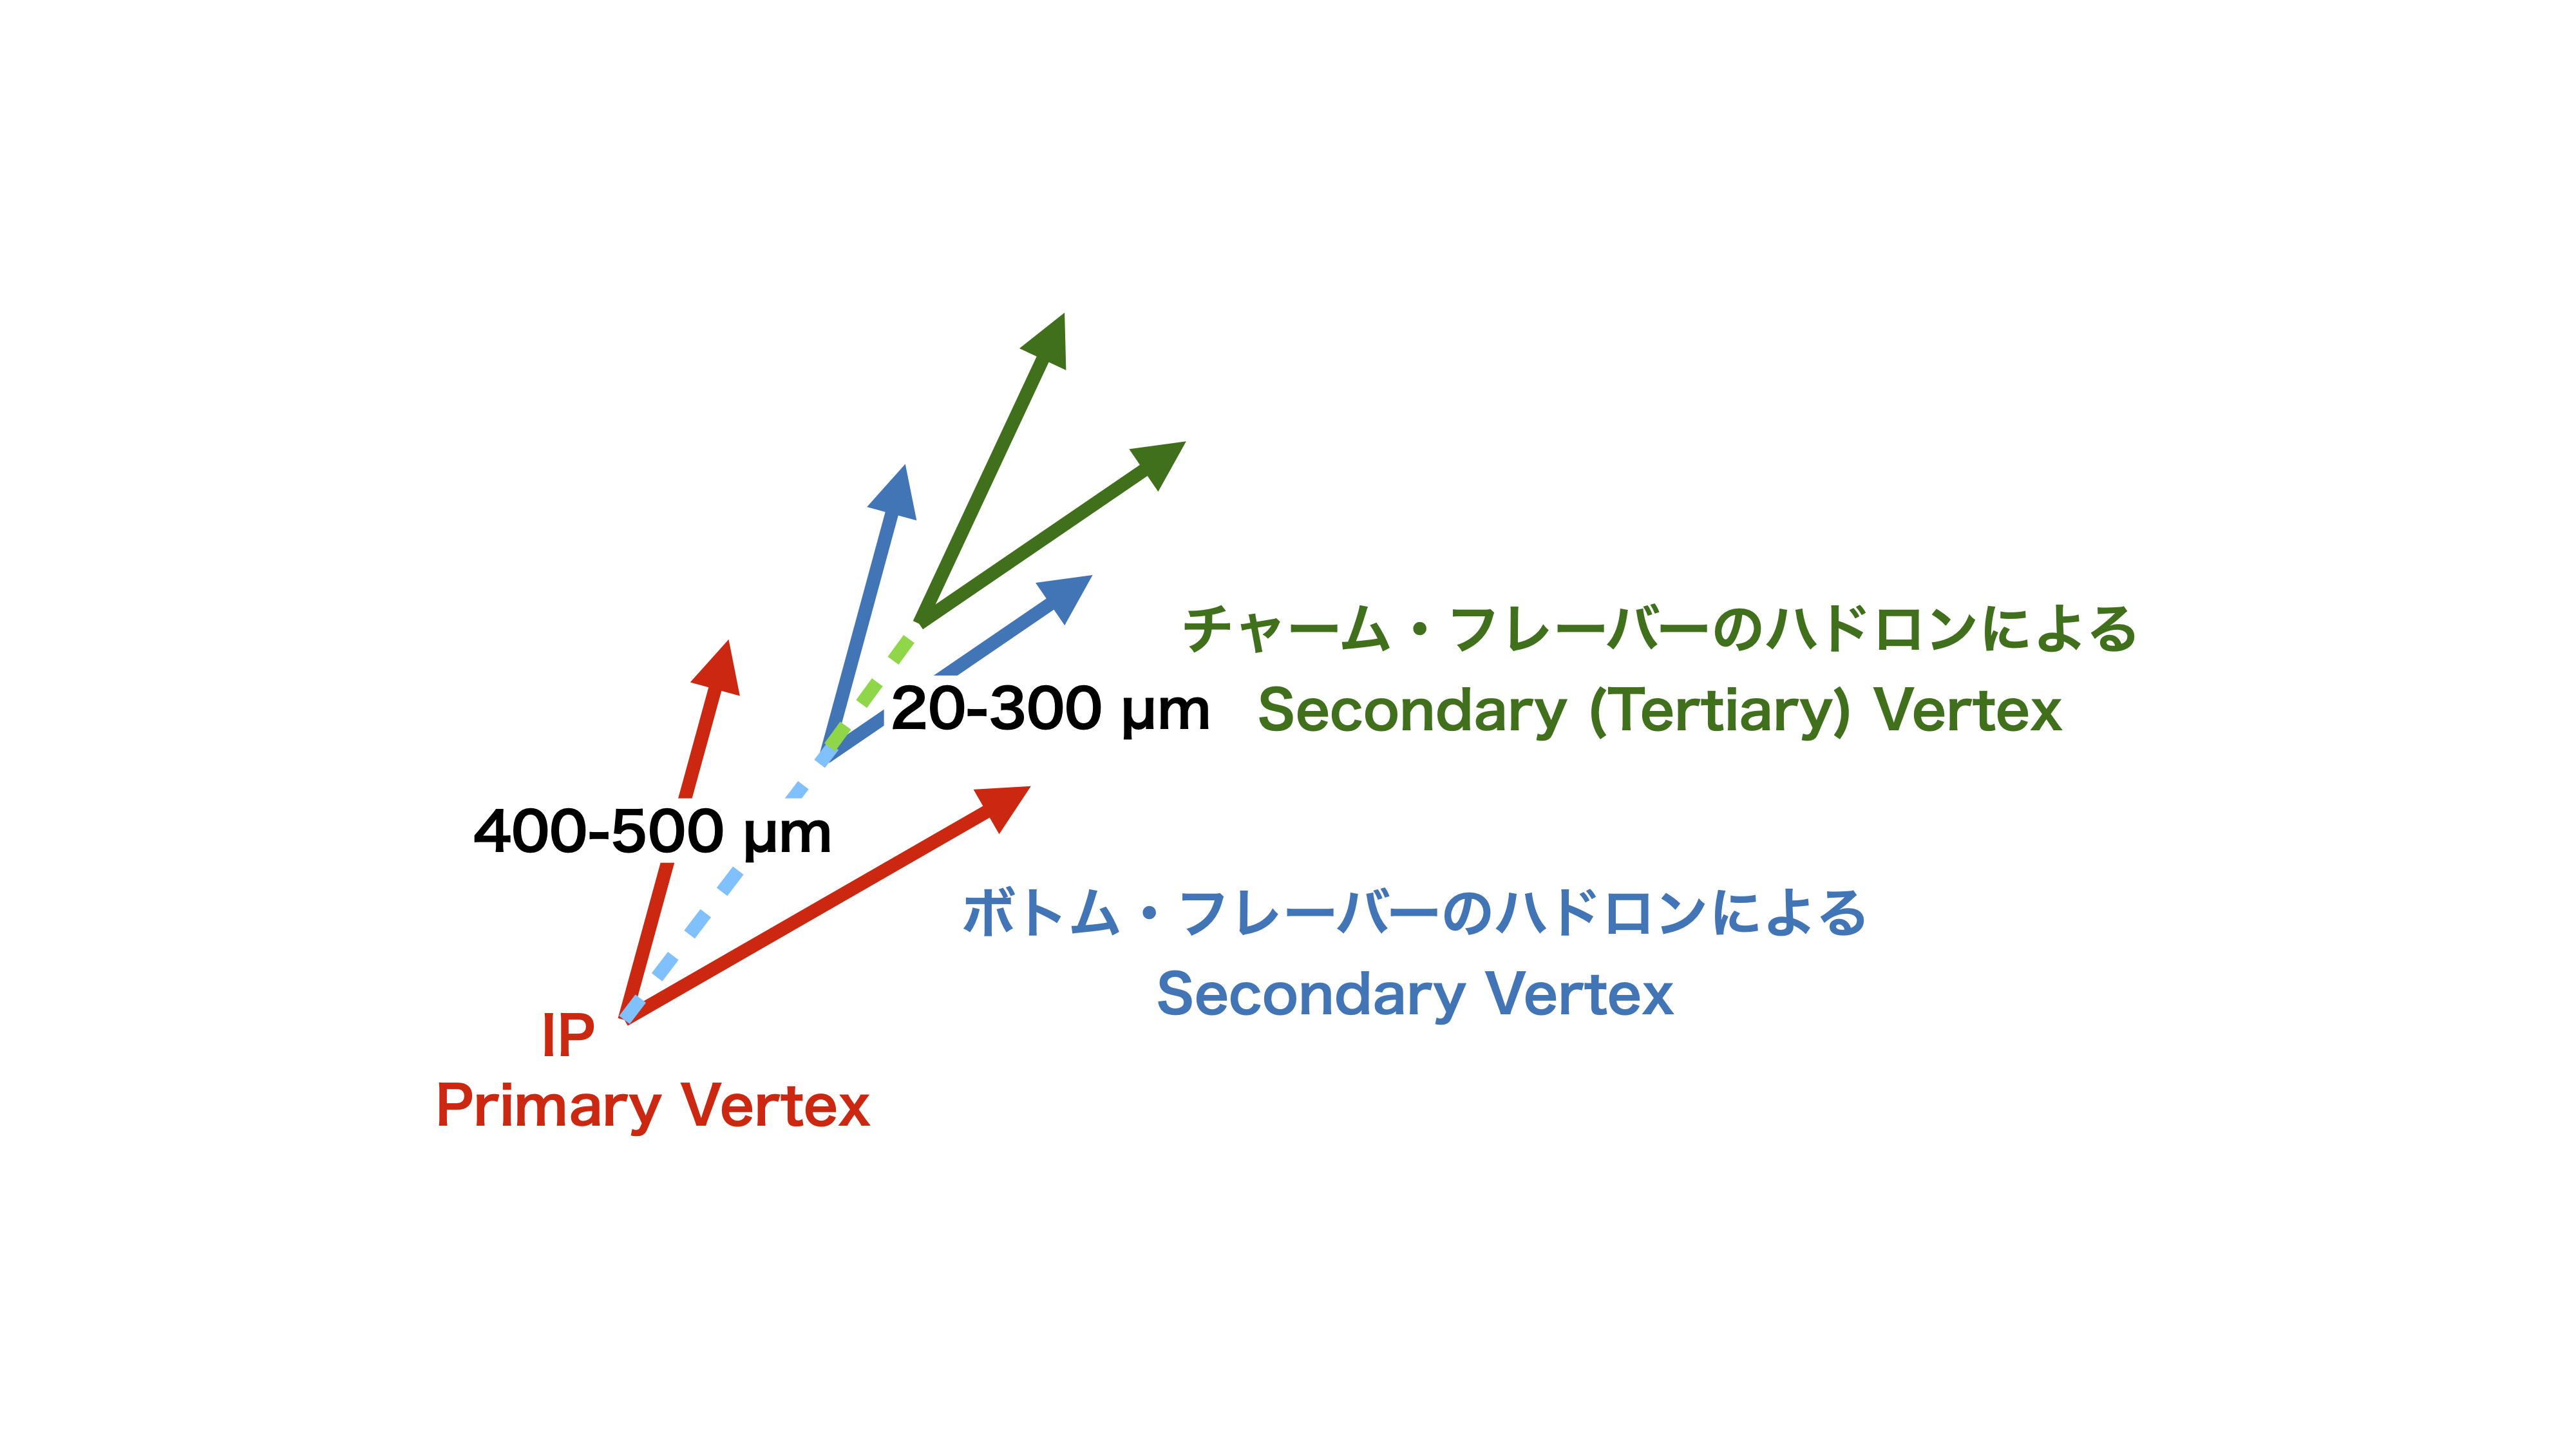
\includegraphics[trim = 200 200 200 200, width=0.9\textwidth, clip]{Figure/3Networks/3-1-1-1FinalStateBB.png}
 \caption[終状態$\rm b\bar{b}$での崩壊点の例]{終状態$\rm b\bar{b}$での崩壊点の例。赤線:Primary Vertex由来の飛跡。青線:Secondary Vertex由来の飛跡。緑線:Tertiary Vertex由来の飛跡。}
 \label{3-1-1-1FinalStateBB}
\end{figure}

また、これら以外の崩壊点としてタウ粒子の崩壊や$\rm V^0$粒子の崩壊 ($\rm K^0_S \to \pi^+\pi^-,\ \Lambda^0 \to p \pi^-$) 、光子変換 ($\rm \gamma_{conv} X \to e^+e^-X$) によるものを考えることができる。
これらの崩壊点はSecondary VertexやTertiary Vertexと比較して、衝突点から遠い位置で生じる。
そのような崩壊点やその崩壊点由来の飛跡を以後Othersと呼ぶ。
図\ref{3-1-1-2TracksandVertices}は一つの事象に含まれる飛跡の本数と崩壊点の個数である。
これらの粒子識別はMC情報を用いた。
ここでは飛跡の本数は親粒子のフレーバーのみ考慮し、同フレーバーの親粒子の違いは区別していない。
したがってSecondary Vertexについては、一つの崩壊点ではなく$\rm b$と$\rm \bar{b}$などの複数の崩壊点の飛跡が含まれている。
親粒子の違いを区別しない場合のSecondary Vertexの飛跡の数は$5$本程度である。
本研究で使用したデータでは、典型的な一事象に含まれる同フレーバーの崩壊点の数は$2$つである。
したがって個々のSecondary Vertexに含まれる飛跡の数は$2-3$本程度となる。
崩壊点検出ではPrimary Vertexと個々のSecondary Vertexを見分ける必要がある。

崩壊点の個数では親粒子を全て区別している。
典型的な崩壊点の個数は終状態が$\rm c\bar{c}$の場合はPrimary Vertex、チャーム・フレーバーのSecondary Vertexが$2$つ、Othersの$3-5$個である。
終状態が$\rm b\bar{b}$の場合はPrimary Vertex、ボトム・フレーバーのSecondary Vertexが$2$つ、チャーム・フレーバーのTertiary Vertexが$2$つ、Othersの$5-7$個である。

\begin{figure}[htbp]
 \centering
 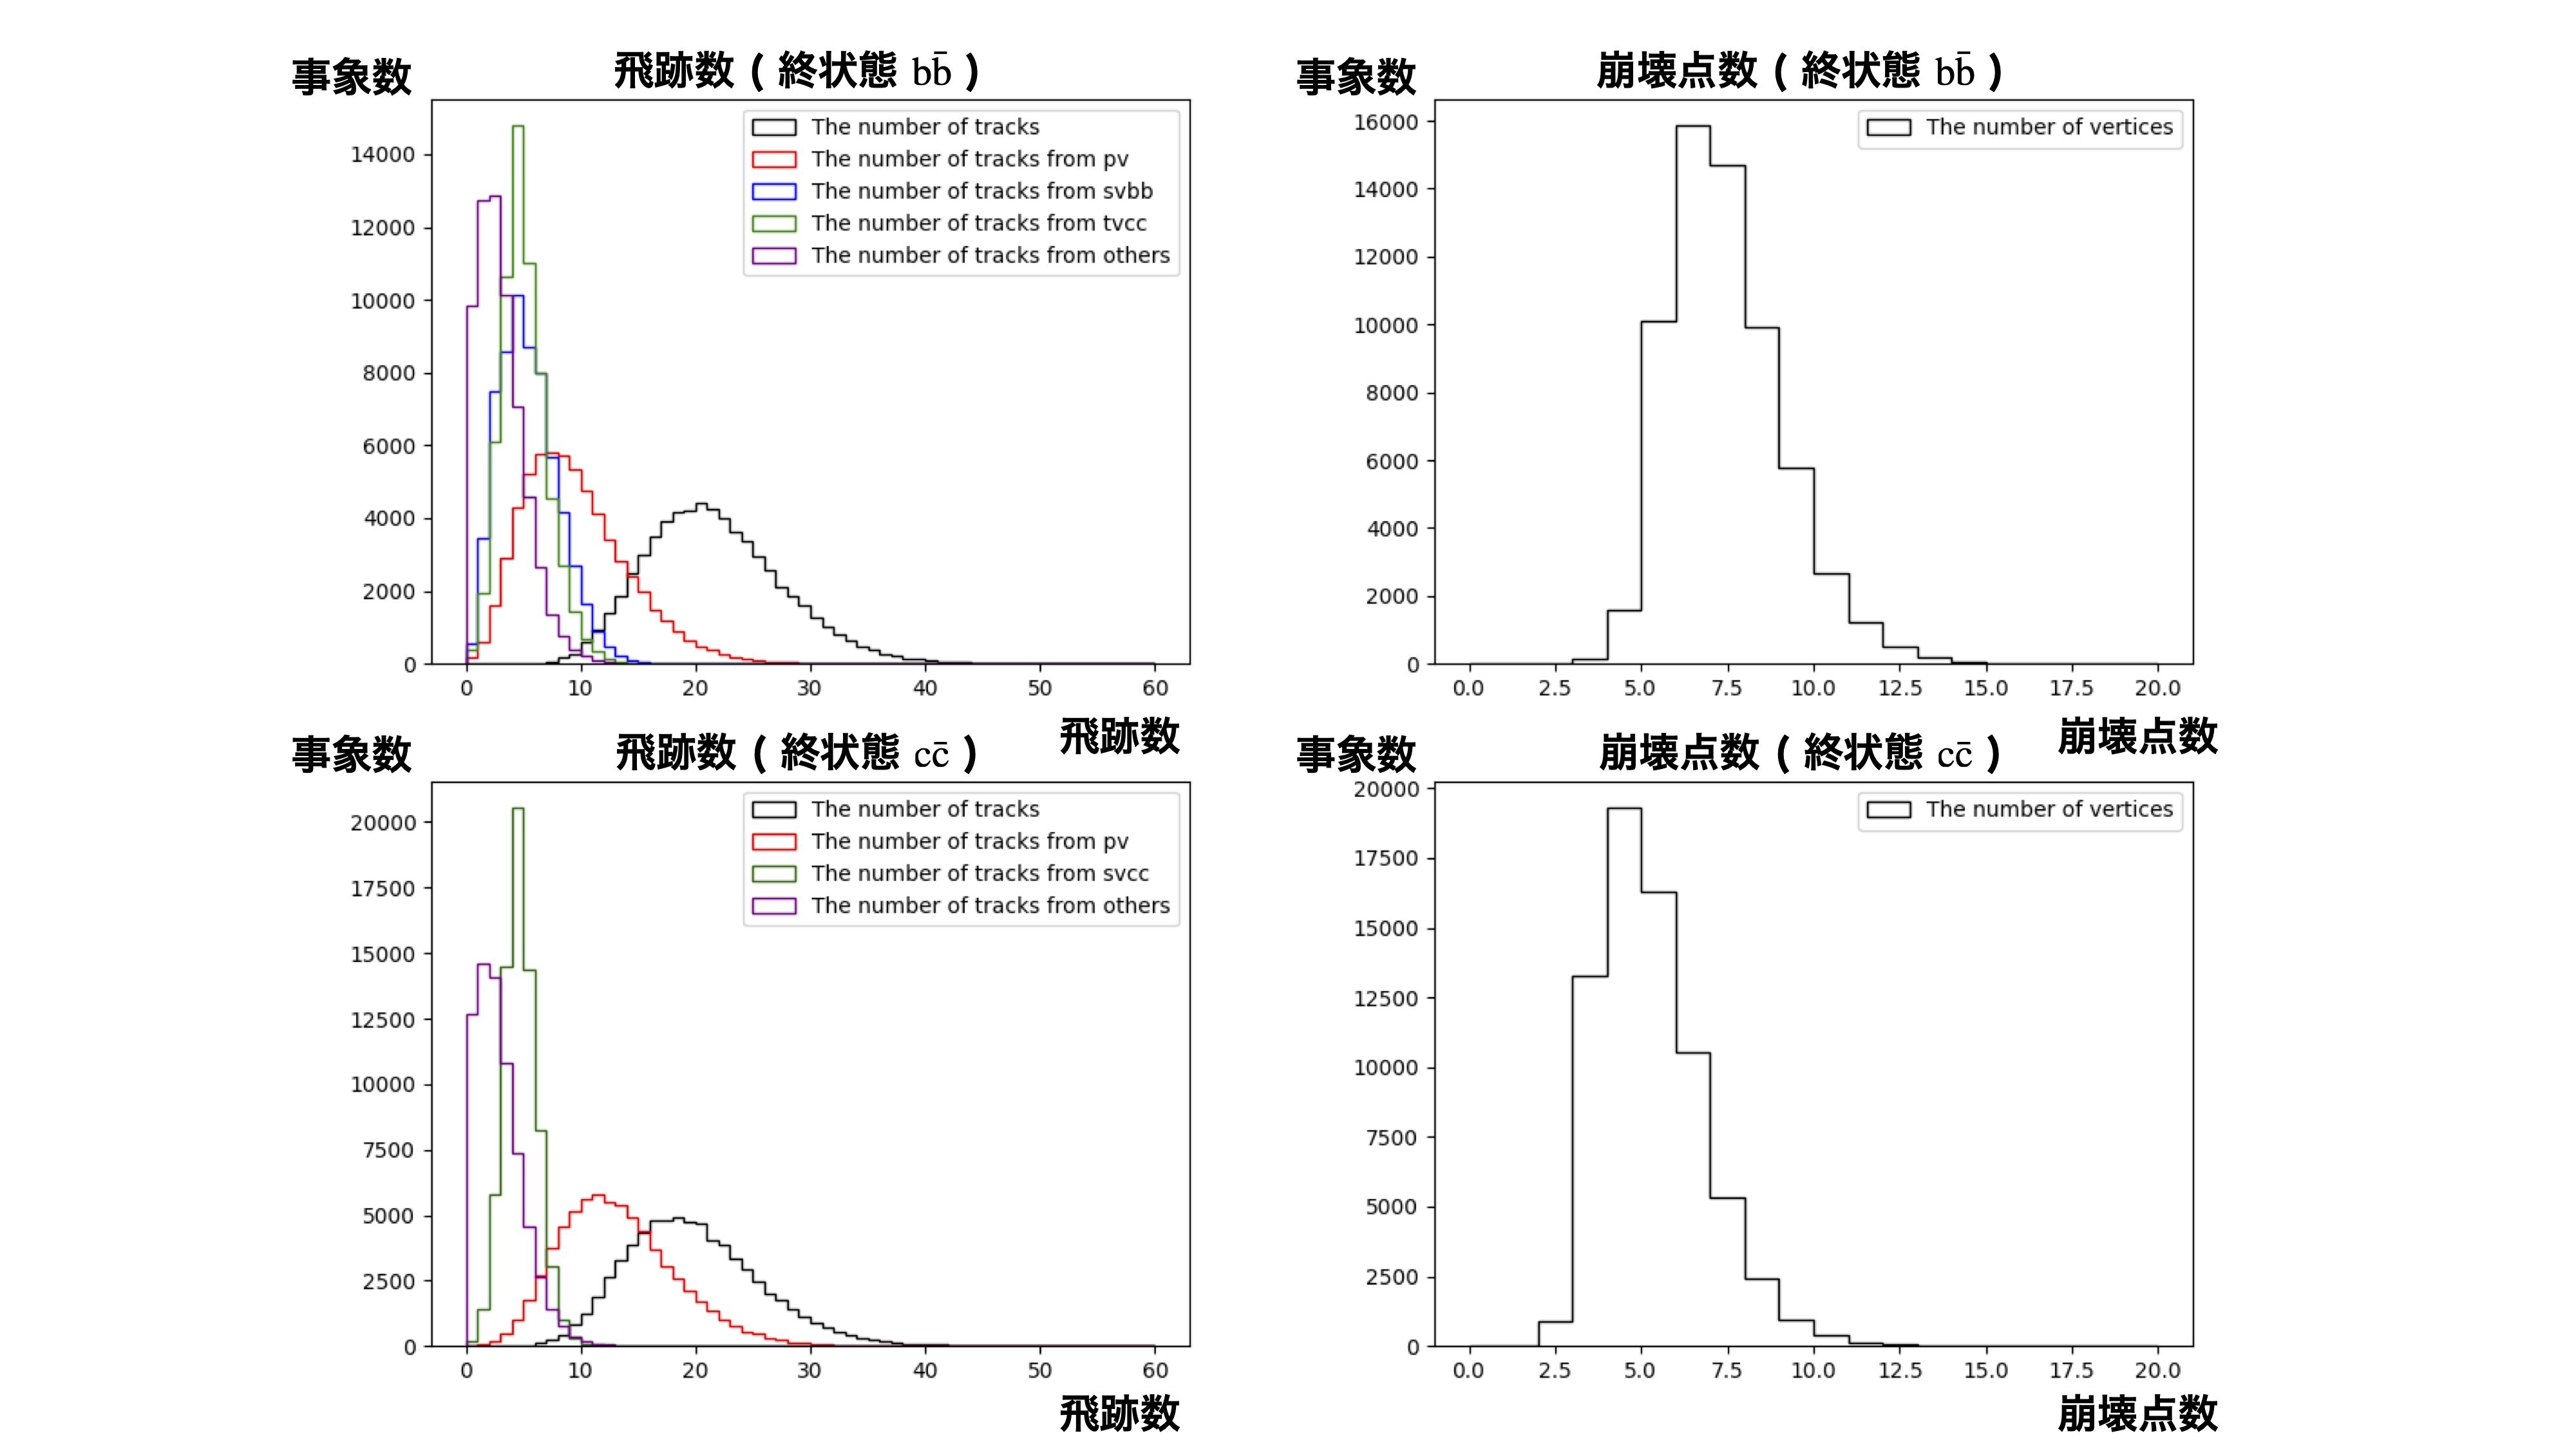
\includegraphics[trim = 150 0 150 0, width=1.0\textwidth, clip]{Figure/3Networks/3-1-1-2TracksandVertices.png}
 \caption[事象に含まれる飛跡の本数と崩壊点の個数]{事象に含まれる飛跡の本数と崩壊点の個数。図左は飛跡の本数、図右は崩壊点の個数である。飛跡の本数において、黒線は事象に含まれる全飛跡数、赤線はPrimary Vertex由来の飛跡数、青線はボトム・フレーバーのSecondary Vertex由来の飛跡数、緑線はチャーム・フレーバーのSecondary Vertex由来の飛跡数、紫線はOthersの飛跡数を表している。}
 \label{3-1-1-2TracksandVertices}
\end{figure}


%%%%%%%%%%%%%%%%%%%%%%%%%%%%%%%%%%%%%%%%%%%%%%%%%%%%%%%%%%%%%%%%%%%%%%%%
\subsection{飛跡の情報と前処理} \label{Net:Data:TrackInformationandPreprocessing}

飛跡一本分の情報として、図\ref{3-1-2-1TrackParameters}のような位置や運動量の情報を含んだトラック・パラメータ$5$個 ($\rm d_0$, $\rm z_0$, $\rm \phi$, $\rm \Omega$, $\rm \tan{\lambda}$)\cite{TrackParametersLCIO}とその共分散行列$15$個、電荷、エネルギーの計$22$個の変数を使用した。
また、加速器の座標系としてビーム衝突点を原点とし、Z軸をビーム方向にとった座標系を使用する。

\begin{figure}[htbp]
 \centering
 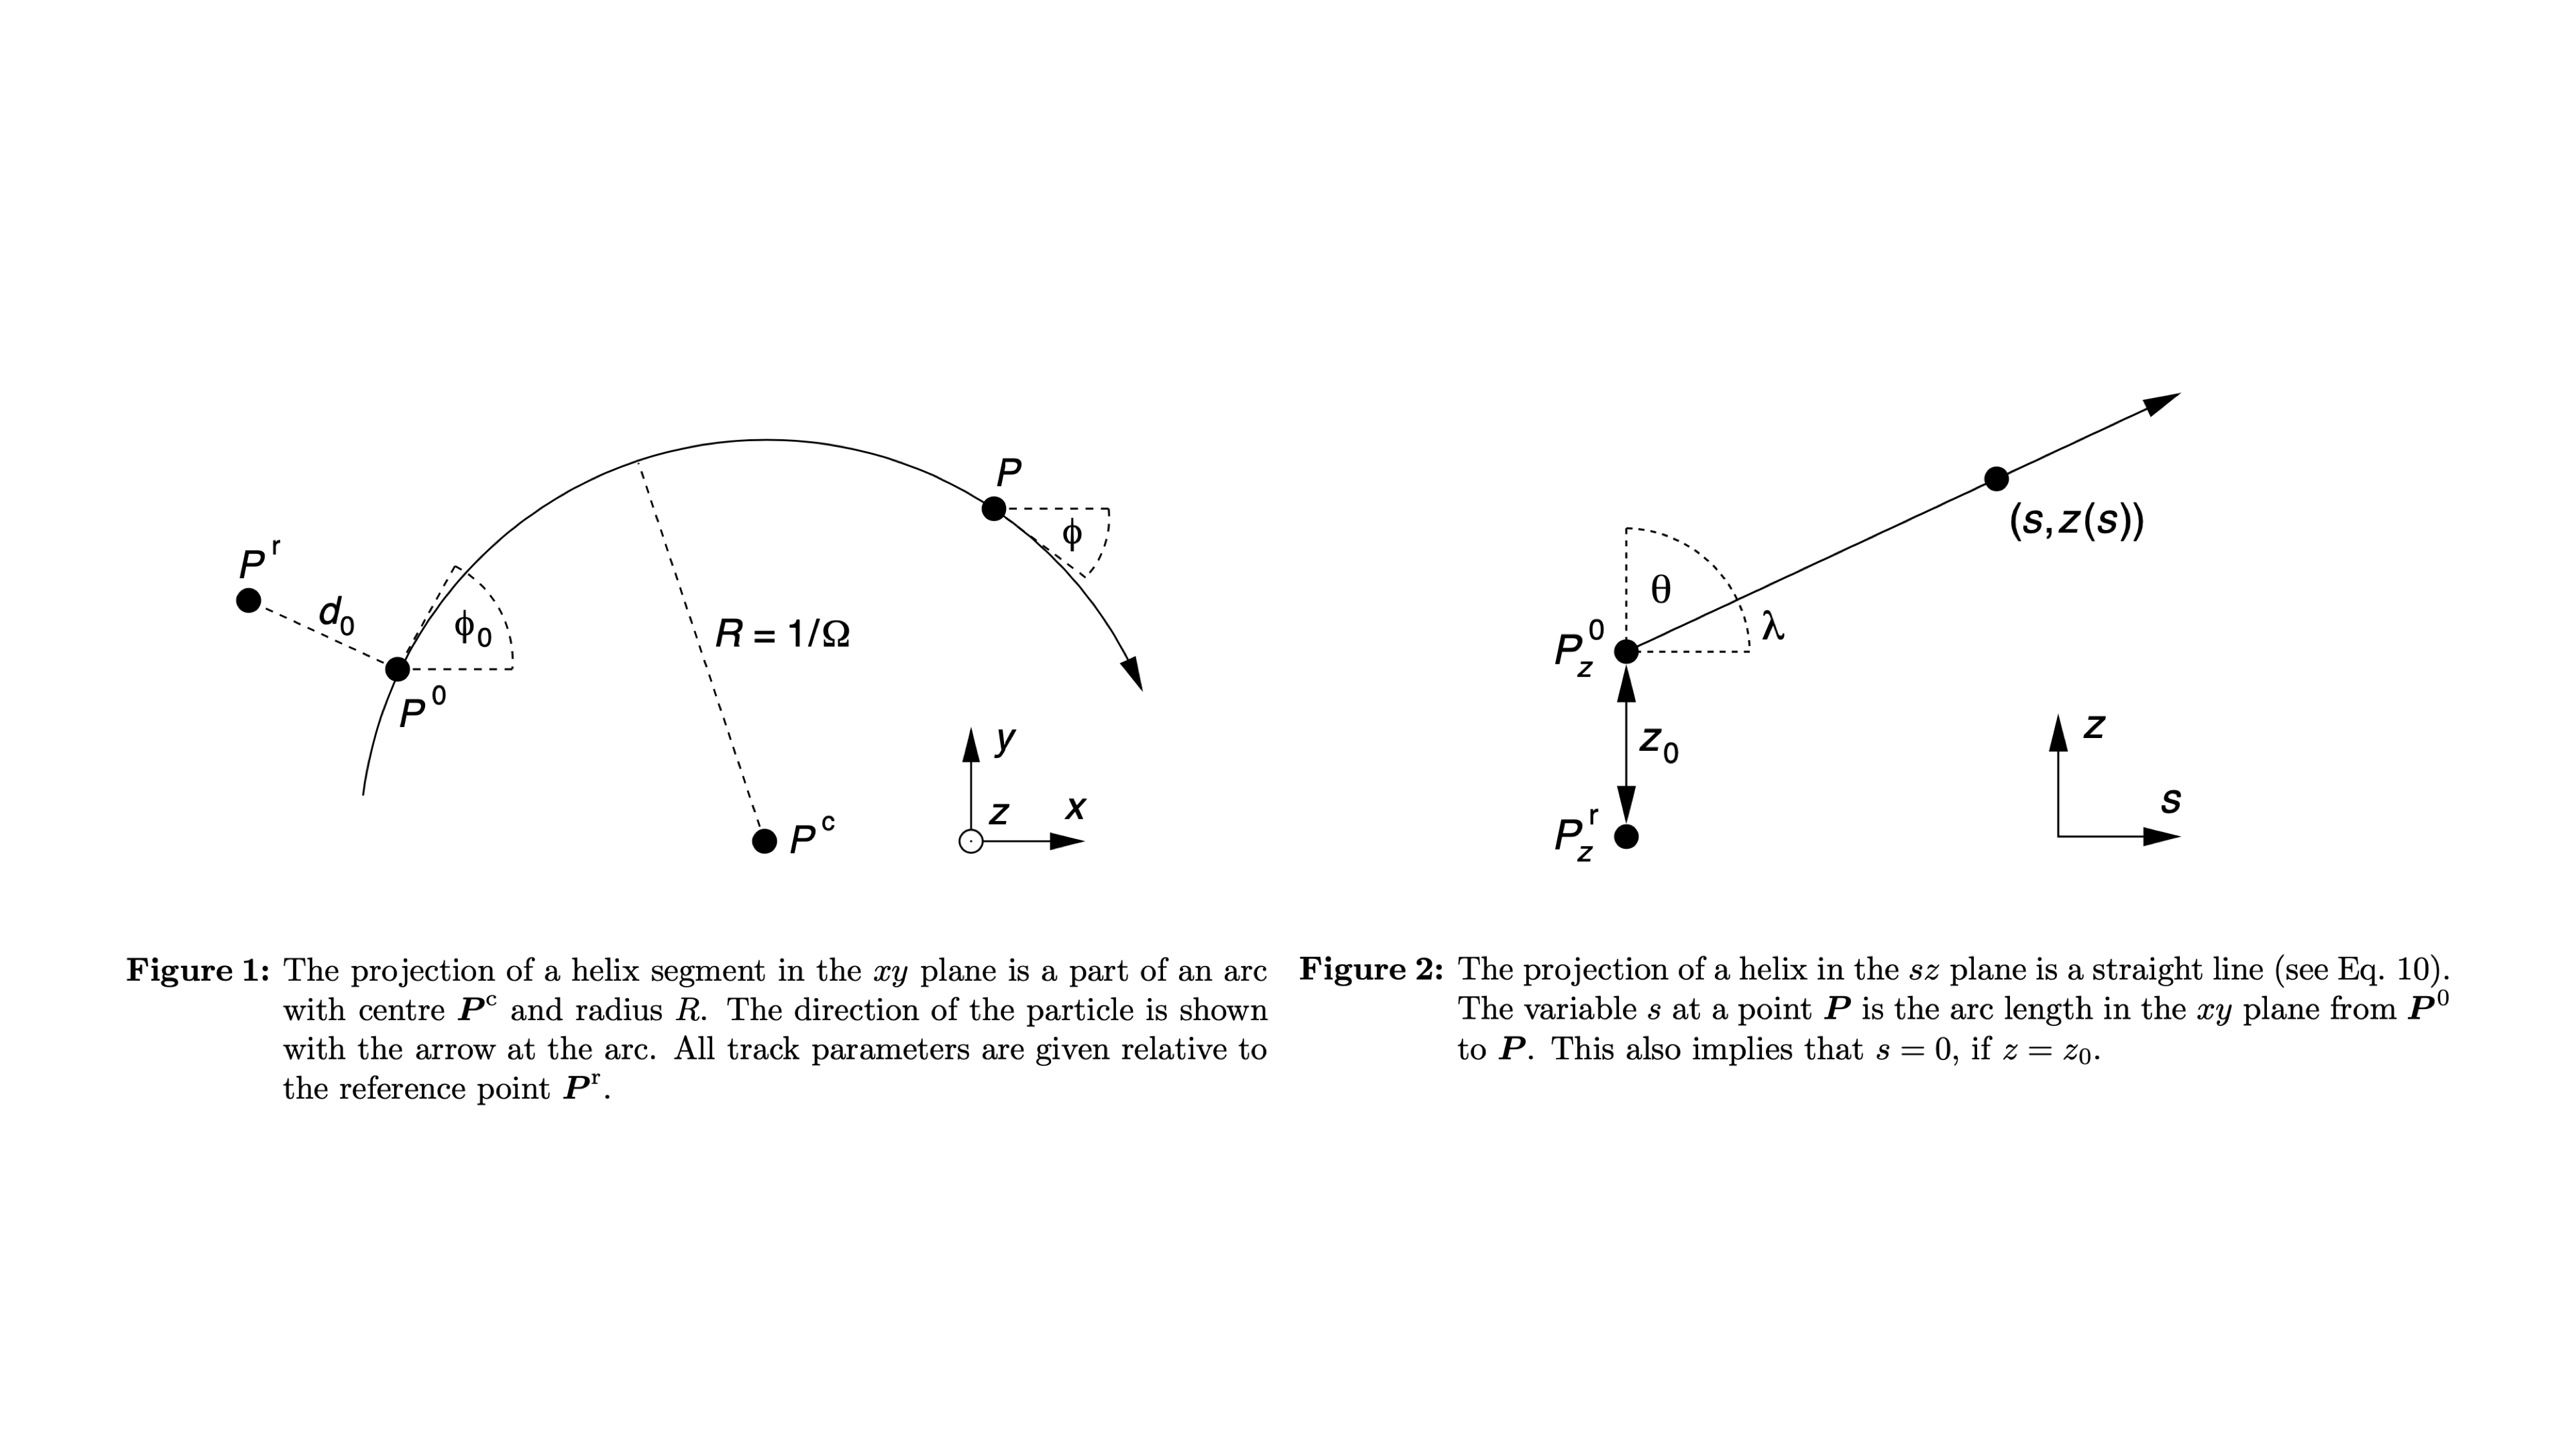
\includegraphics[trim = 50 150 50 250, width=1.0\textwidth, clip]{Figure/3Networks/3-1-2-1TrackParameters.png}
 \caption[トラック・パラメータの定義]{トラック・パラメータの定義\cite{TrackParametersLCIO}}
 \label{3-1-2-1TrackParameters}
\end{figure}

深層学習の入力に使用する変数は、一般に$[-1,\ 1]$の範囲に整形した方が良いと言われている為、変数をそれぞれ以下のような$\tanh$関数や線形関数などを用いて整形した。

\begin{itemize}
 \item トラック・パラメータ\\
 ${\rm d_0} = \tanh{({\rm d_0})}$,
 ${\rm z_0} = \tanh{({\rm z_0})}$,
 ${\rm \phi} = {\rm \phi}/\pi$,
 ${\rm \Omega} = \tanh{(200\ {\rm \Omega})}$,
 ${\rm \tan{\lambda}} = \tanh{(0.3\ {\rm \tan{\lambda}})}$
 \item トラック・パラメータの共分散行列\\
 $\tanh{(8000\ (x-0.0005))}$
 \item エネルギー\\
 $\tanh{(0.5\ (x-5.0))}$
\end{itemize}

トラック・パラメータとエネルギーの整形前と整形後の分布をそれぞれ図\ref{3-1-2-2Variables}に示す。
整形後の変数の分布が$[-1,\ 1]$の範囲になっていることがわかる。

\begin{figure}[htbp]
 \centering
  %\begin{tabular}{cccc}
  \begin{minipage}{1.0\textwidth}
  \centering
   \begin{minipage}{0.48\textwidth}
    \centering
    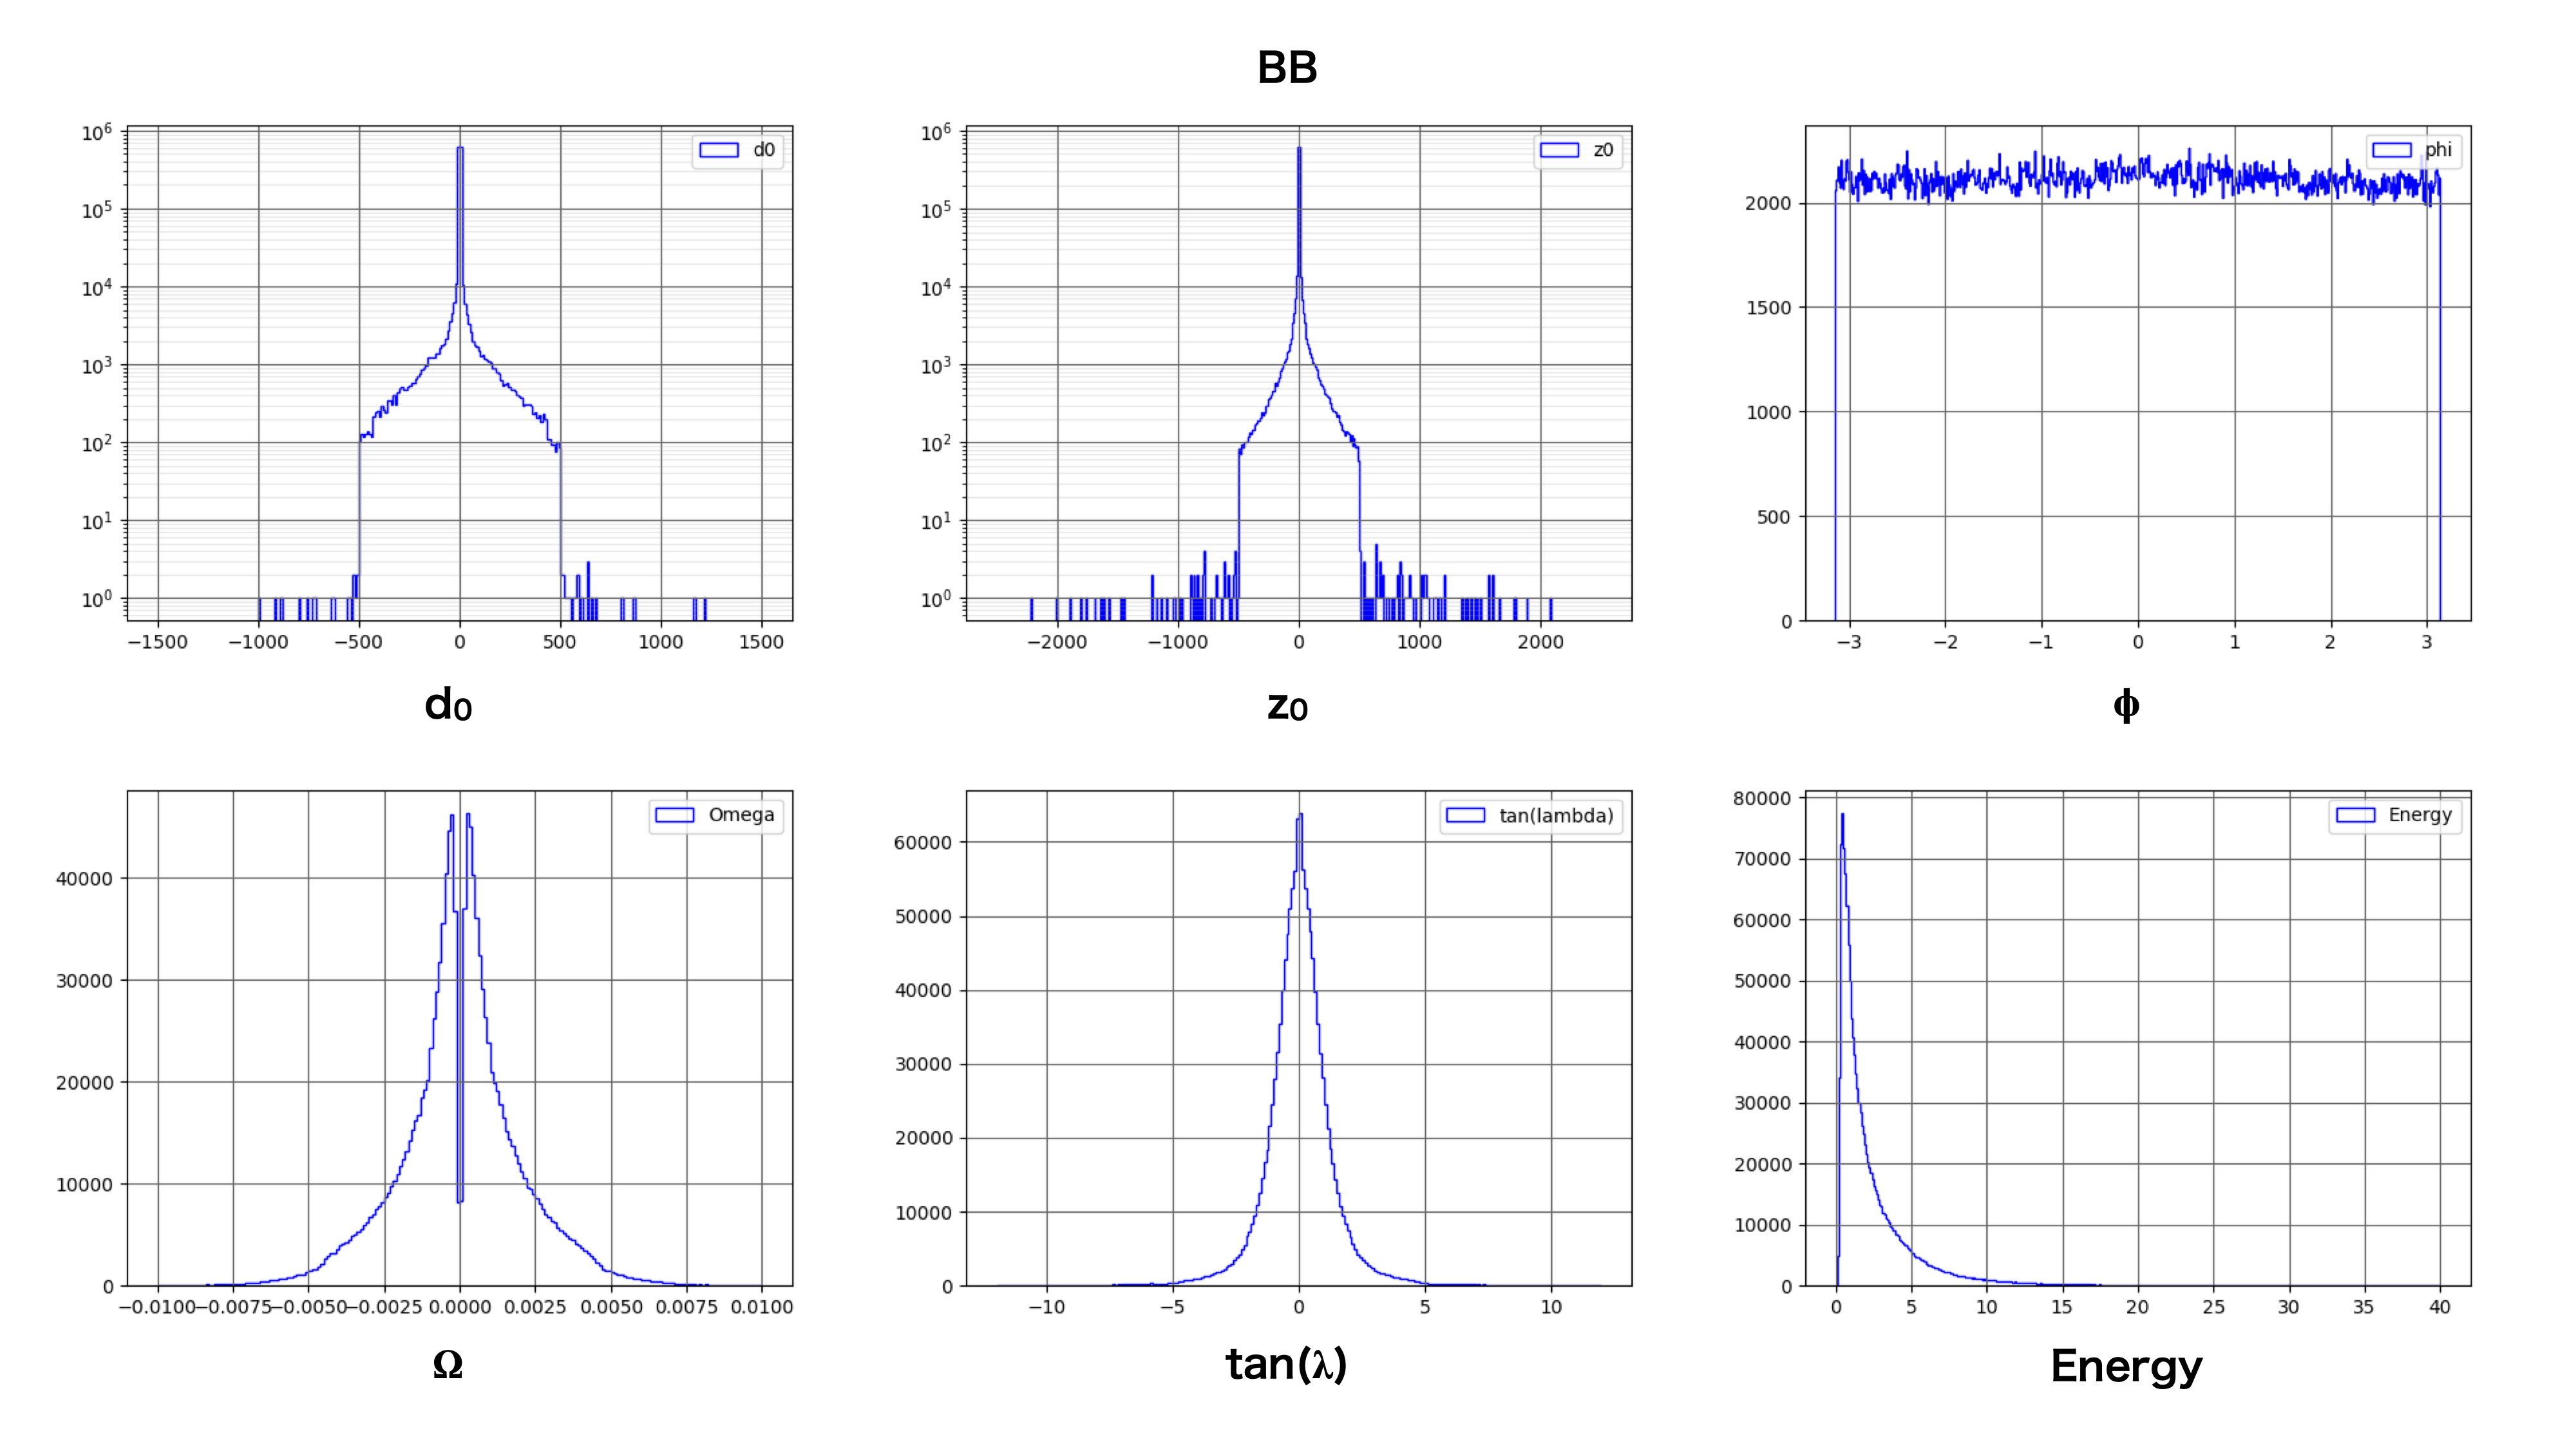
\includegraphics[width=1.0\textwidth, clip]{Figure/3Networks/3-1-2-2OriginalVariablesBB.png}
    \subcaption{終状態$\rm b\bar{b}$での変換前の変数の分布}
    \label{3-1-2-2OriginalVariablesBB}
   \end{minipage}
   \begin{minipage}{0.48\textwidth}
   \centering
    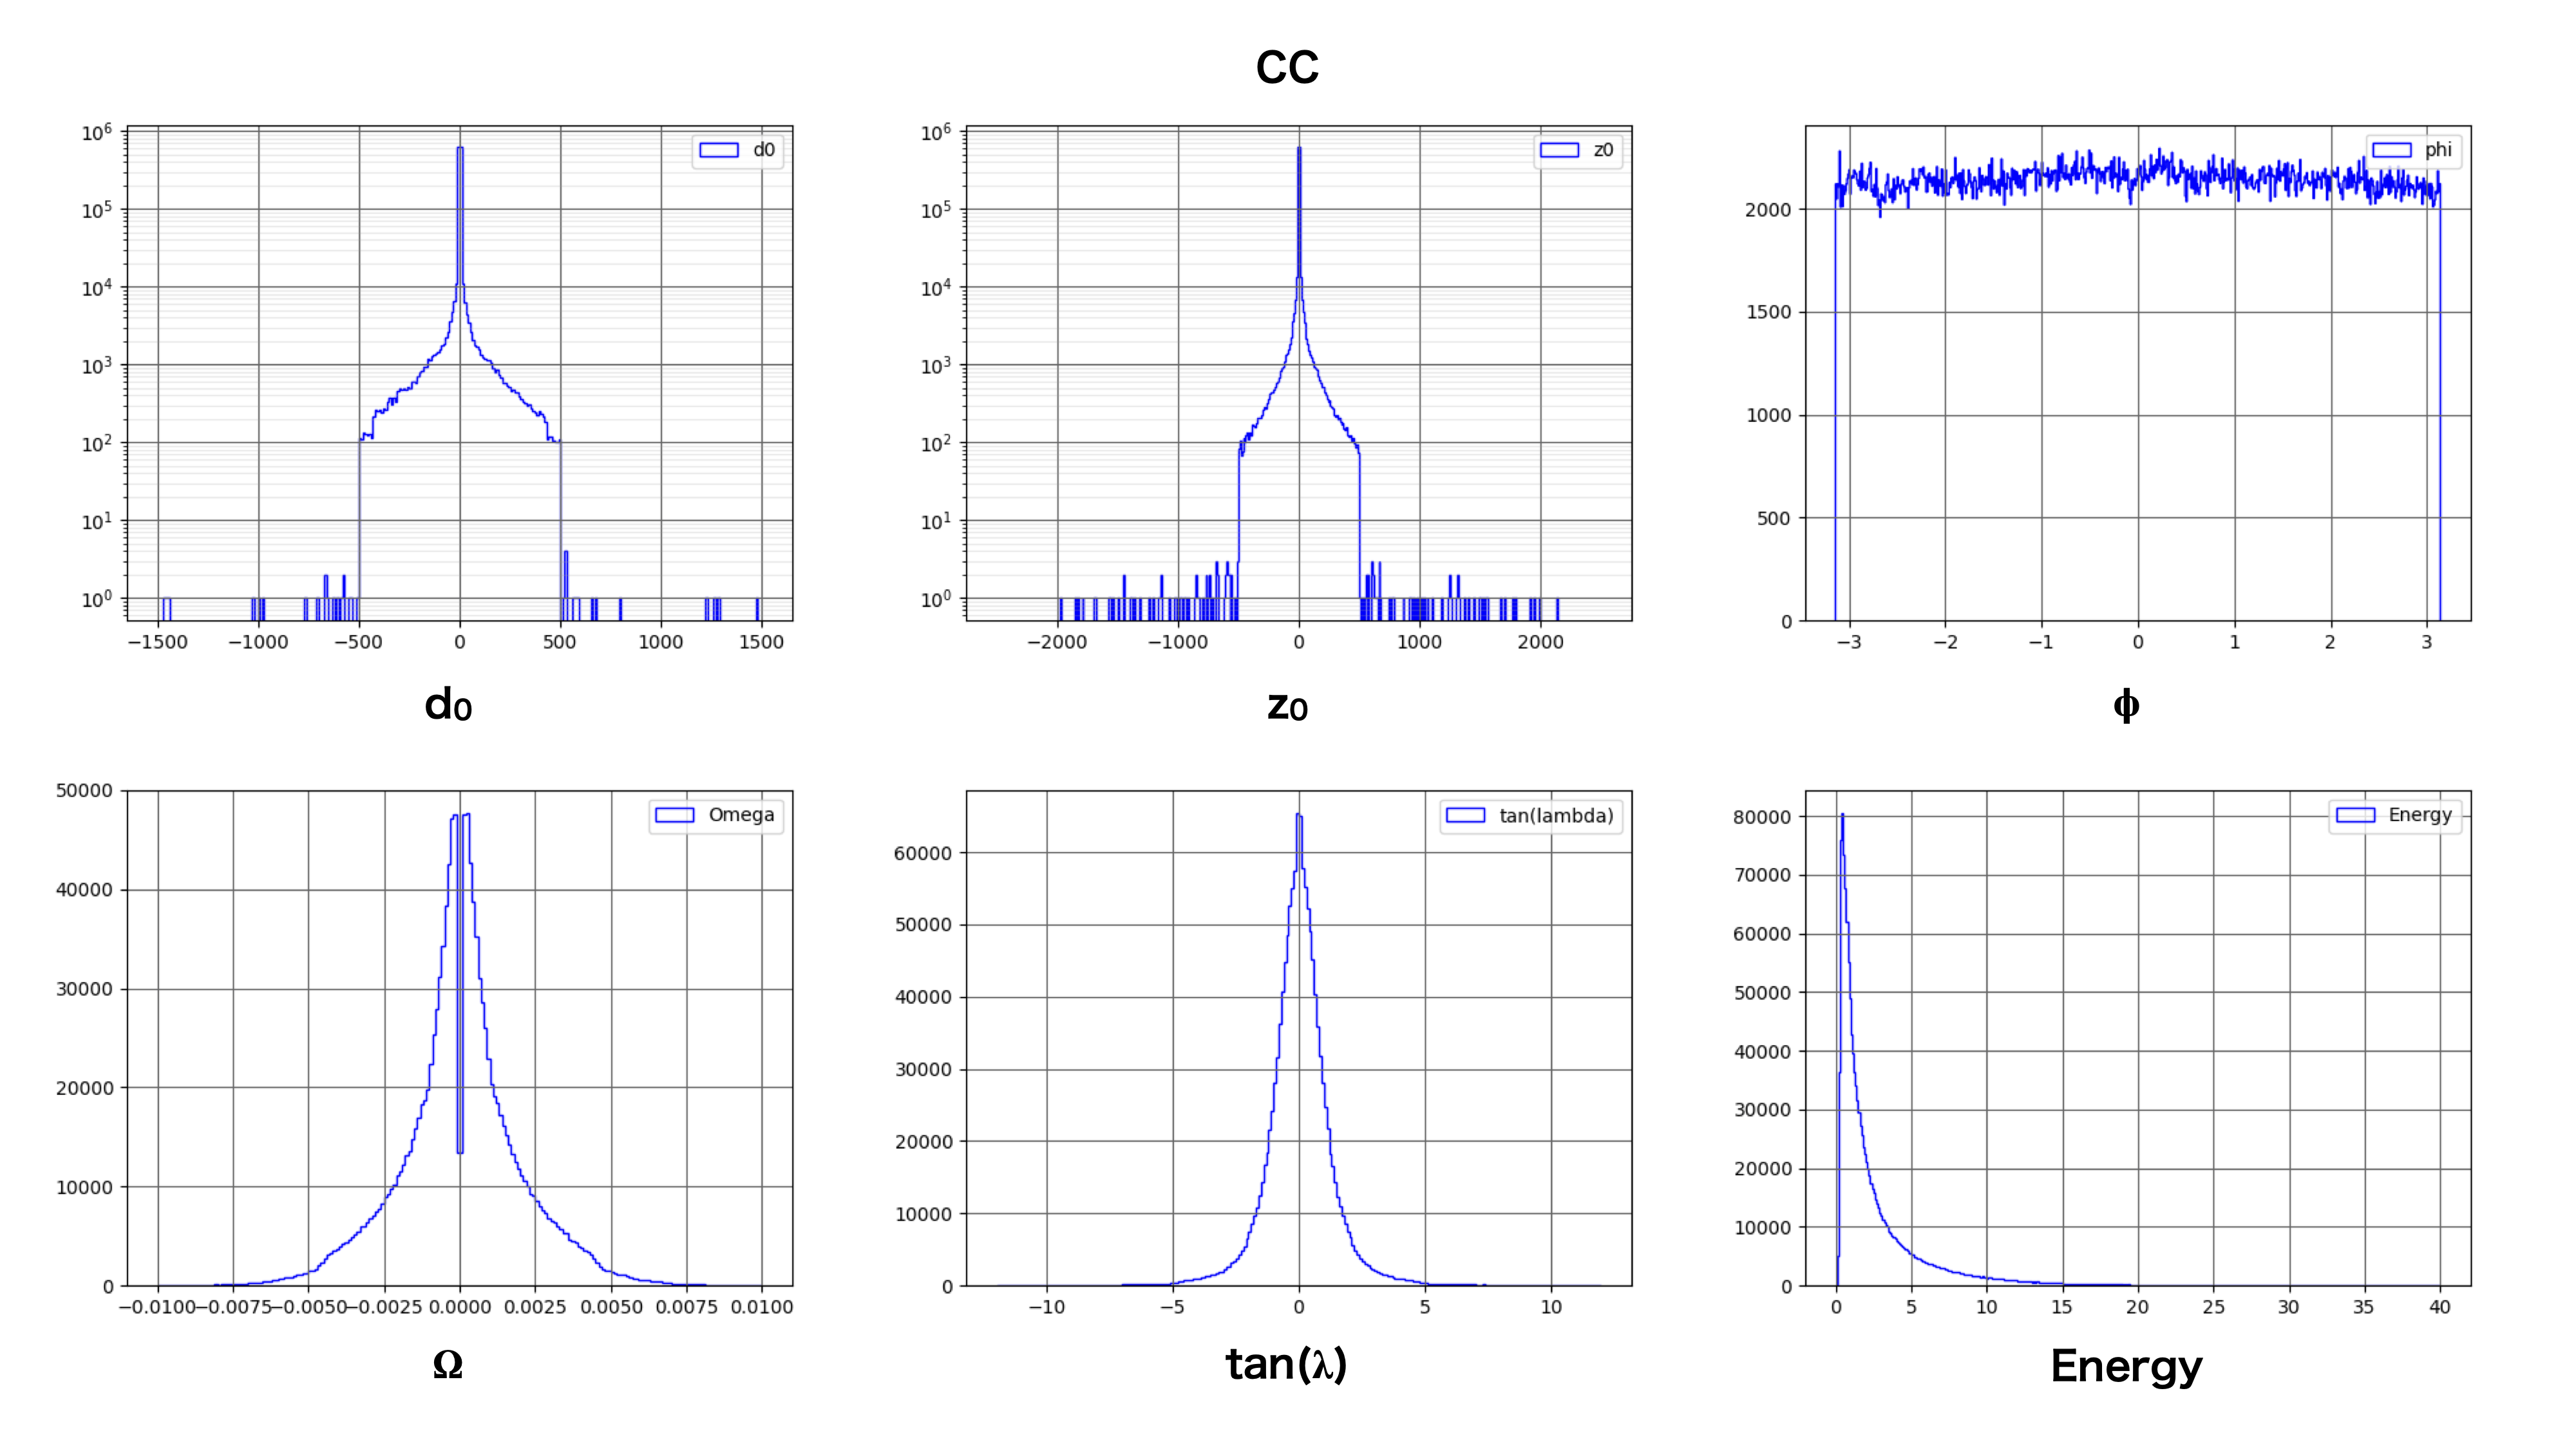
\includegraphics[width=1.0\textwidth, clip]{Figure/3Networks/3-1-2-2OriginalVariablesCC.png}
    \subcaption{終状態$\rm c\bar{c}$での変換前の変数の分布}
    \label{3-1-2-2OriginalVariablesCC}
   \end{minipage}
  \end{minipage}
  
  \begin{minipage}{1.0\textwidth}
  \centering
   \begin{minipage}{0.48\textwidth}
   \centering
    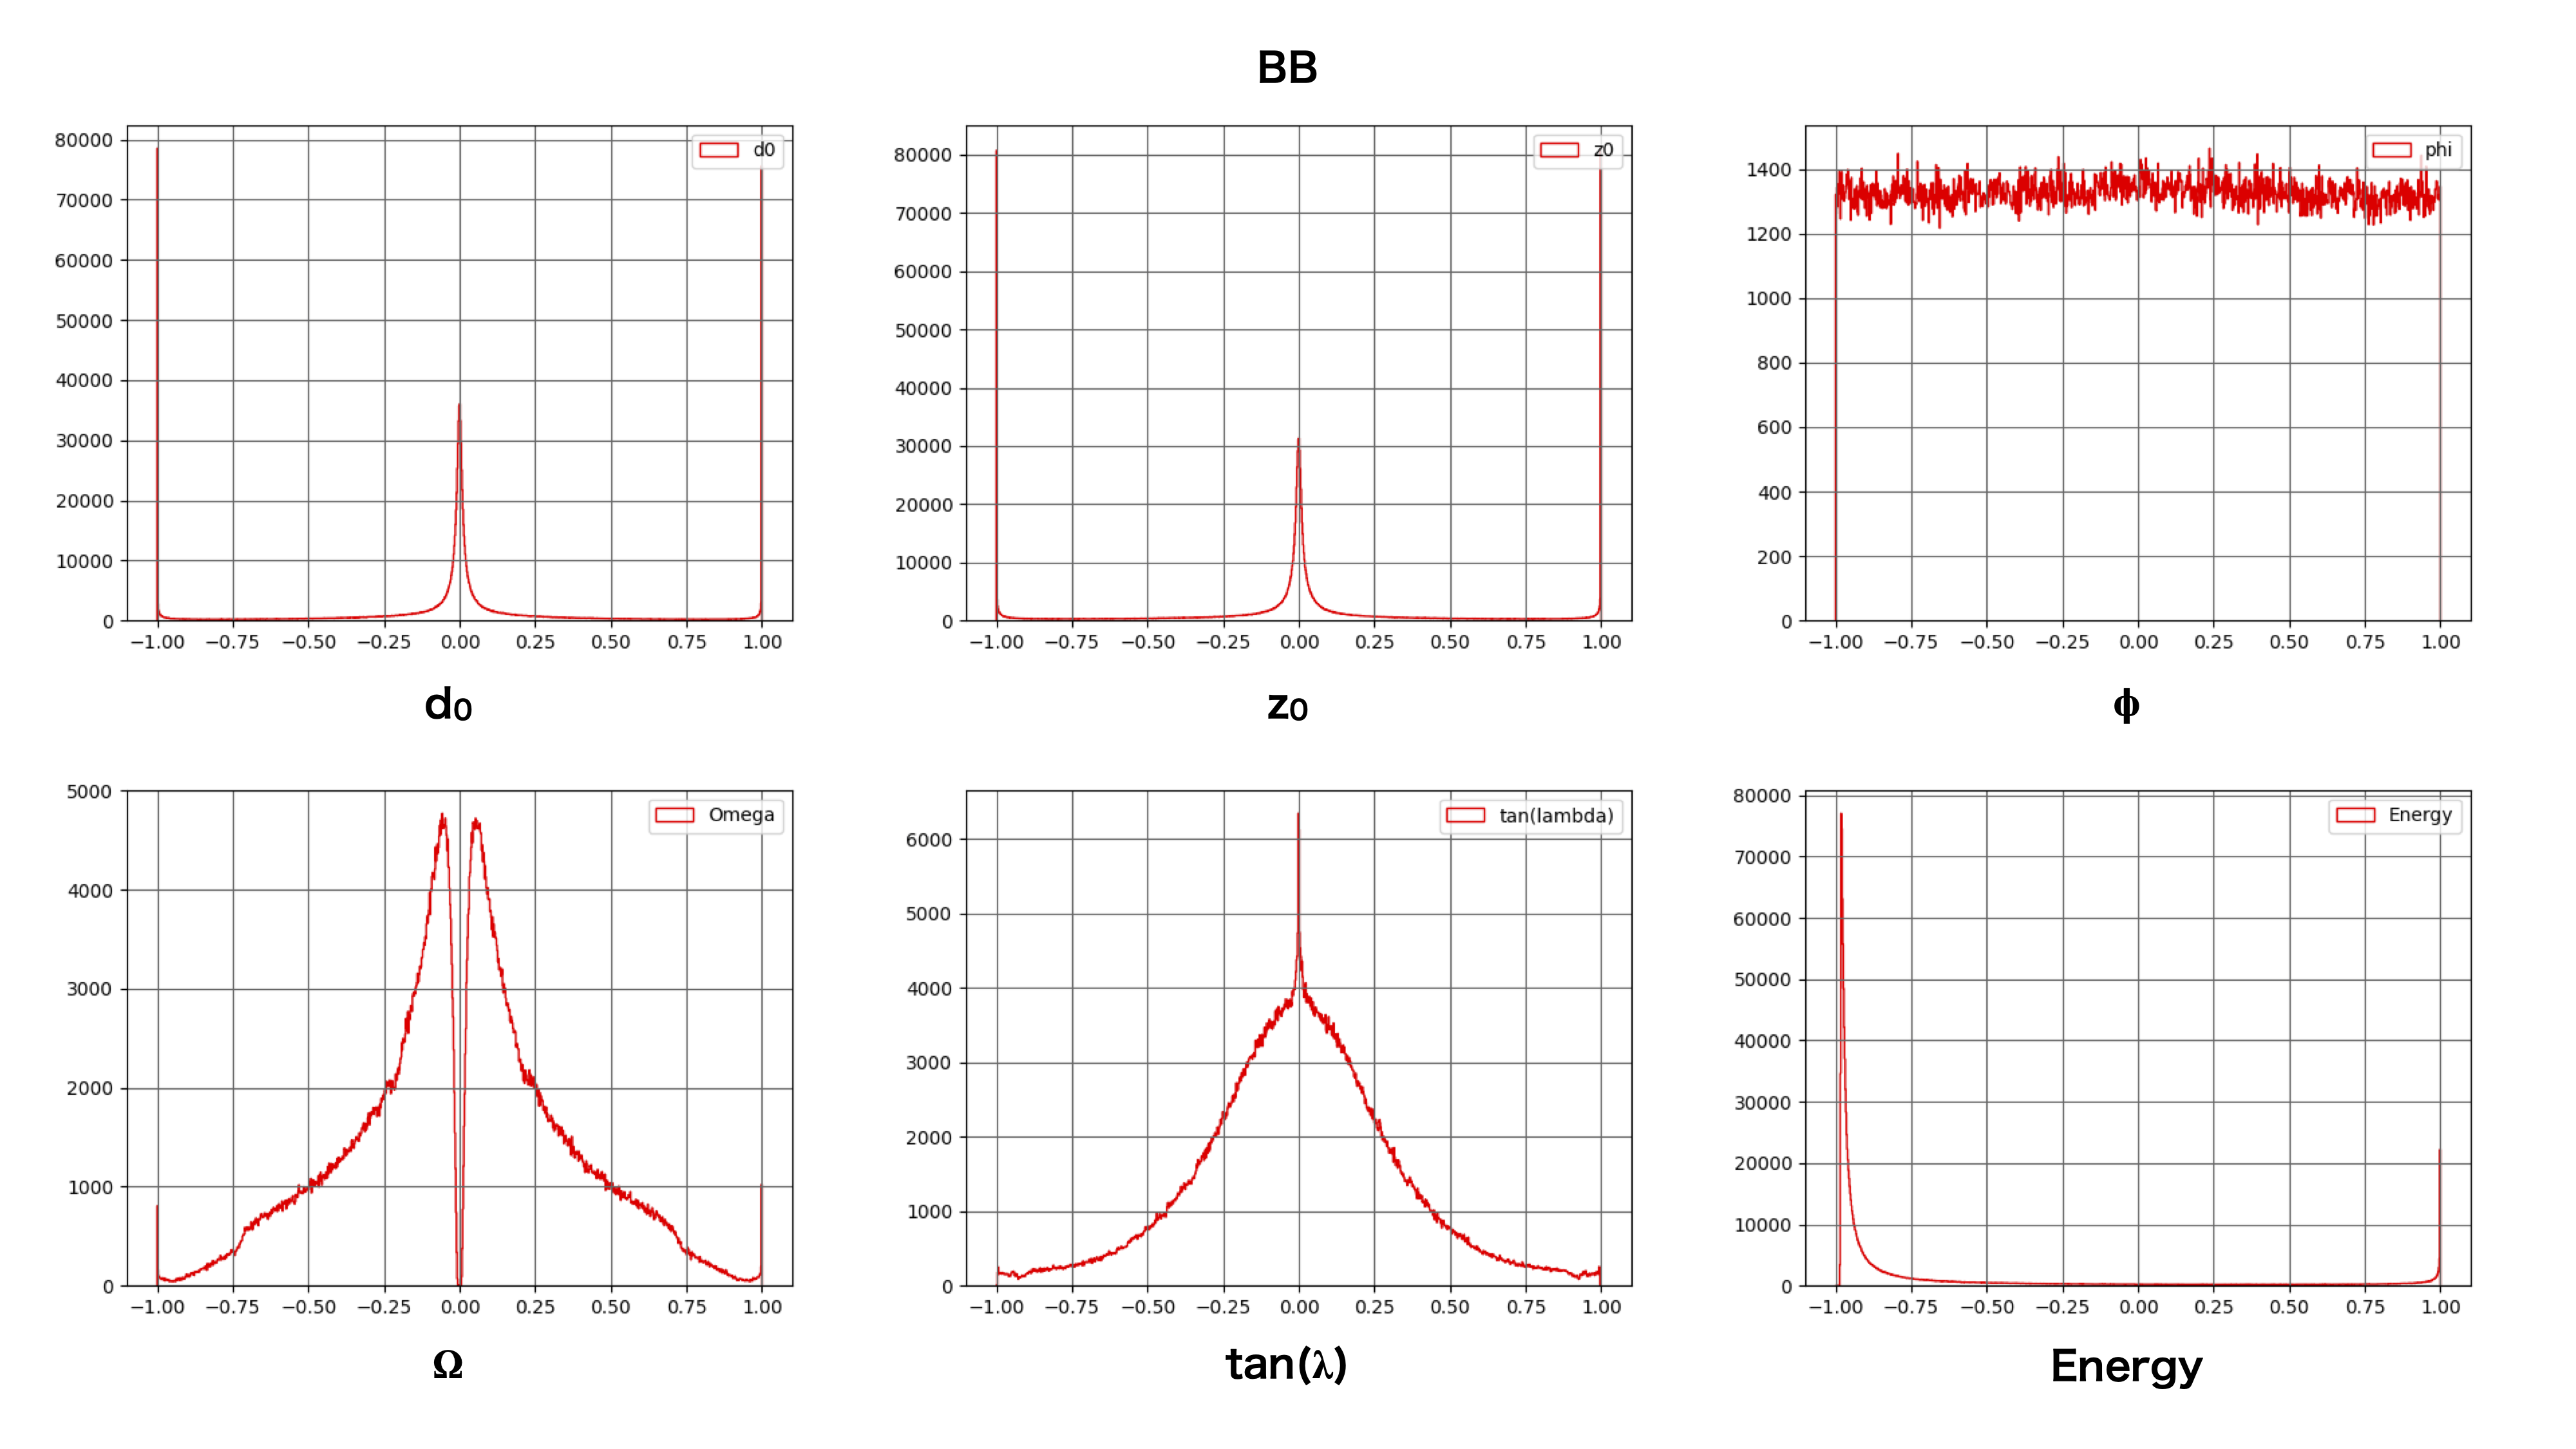
\includegraphics[width=1.0\textwidth, clip]{Figure/3Networks/3-1-2-2ReshapedVariablesBB.png}
    \subcaption{終状態$\rm b\bar{b}$での変換後の変数の分布}
    \label{3-1-2-2ReshapedVariablesBB}
   \end{minipage}
   \begin{minipage}{0.48\textwidth}
   \centering
    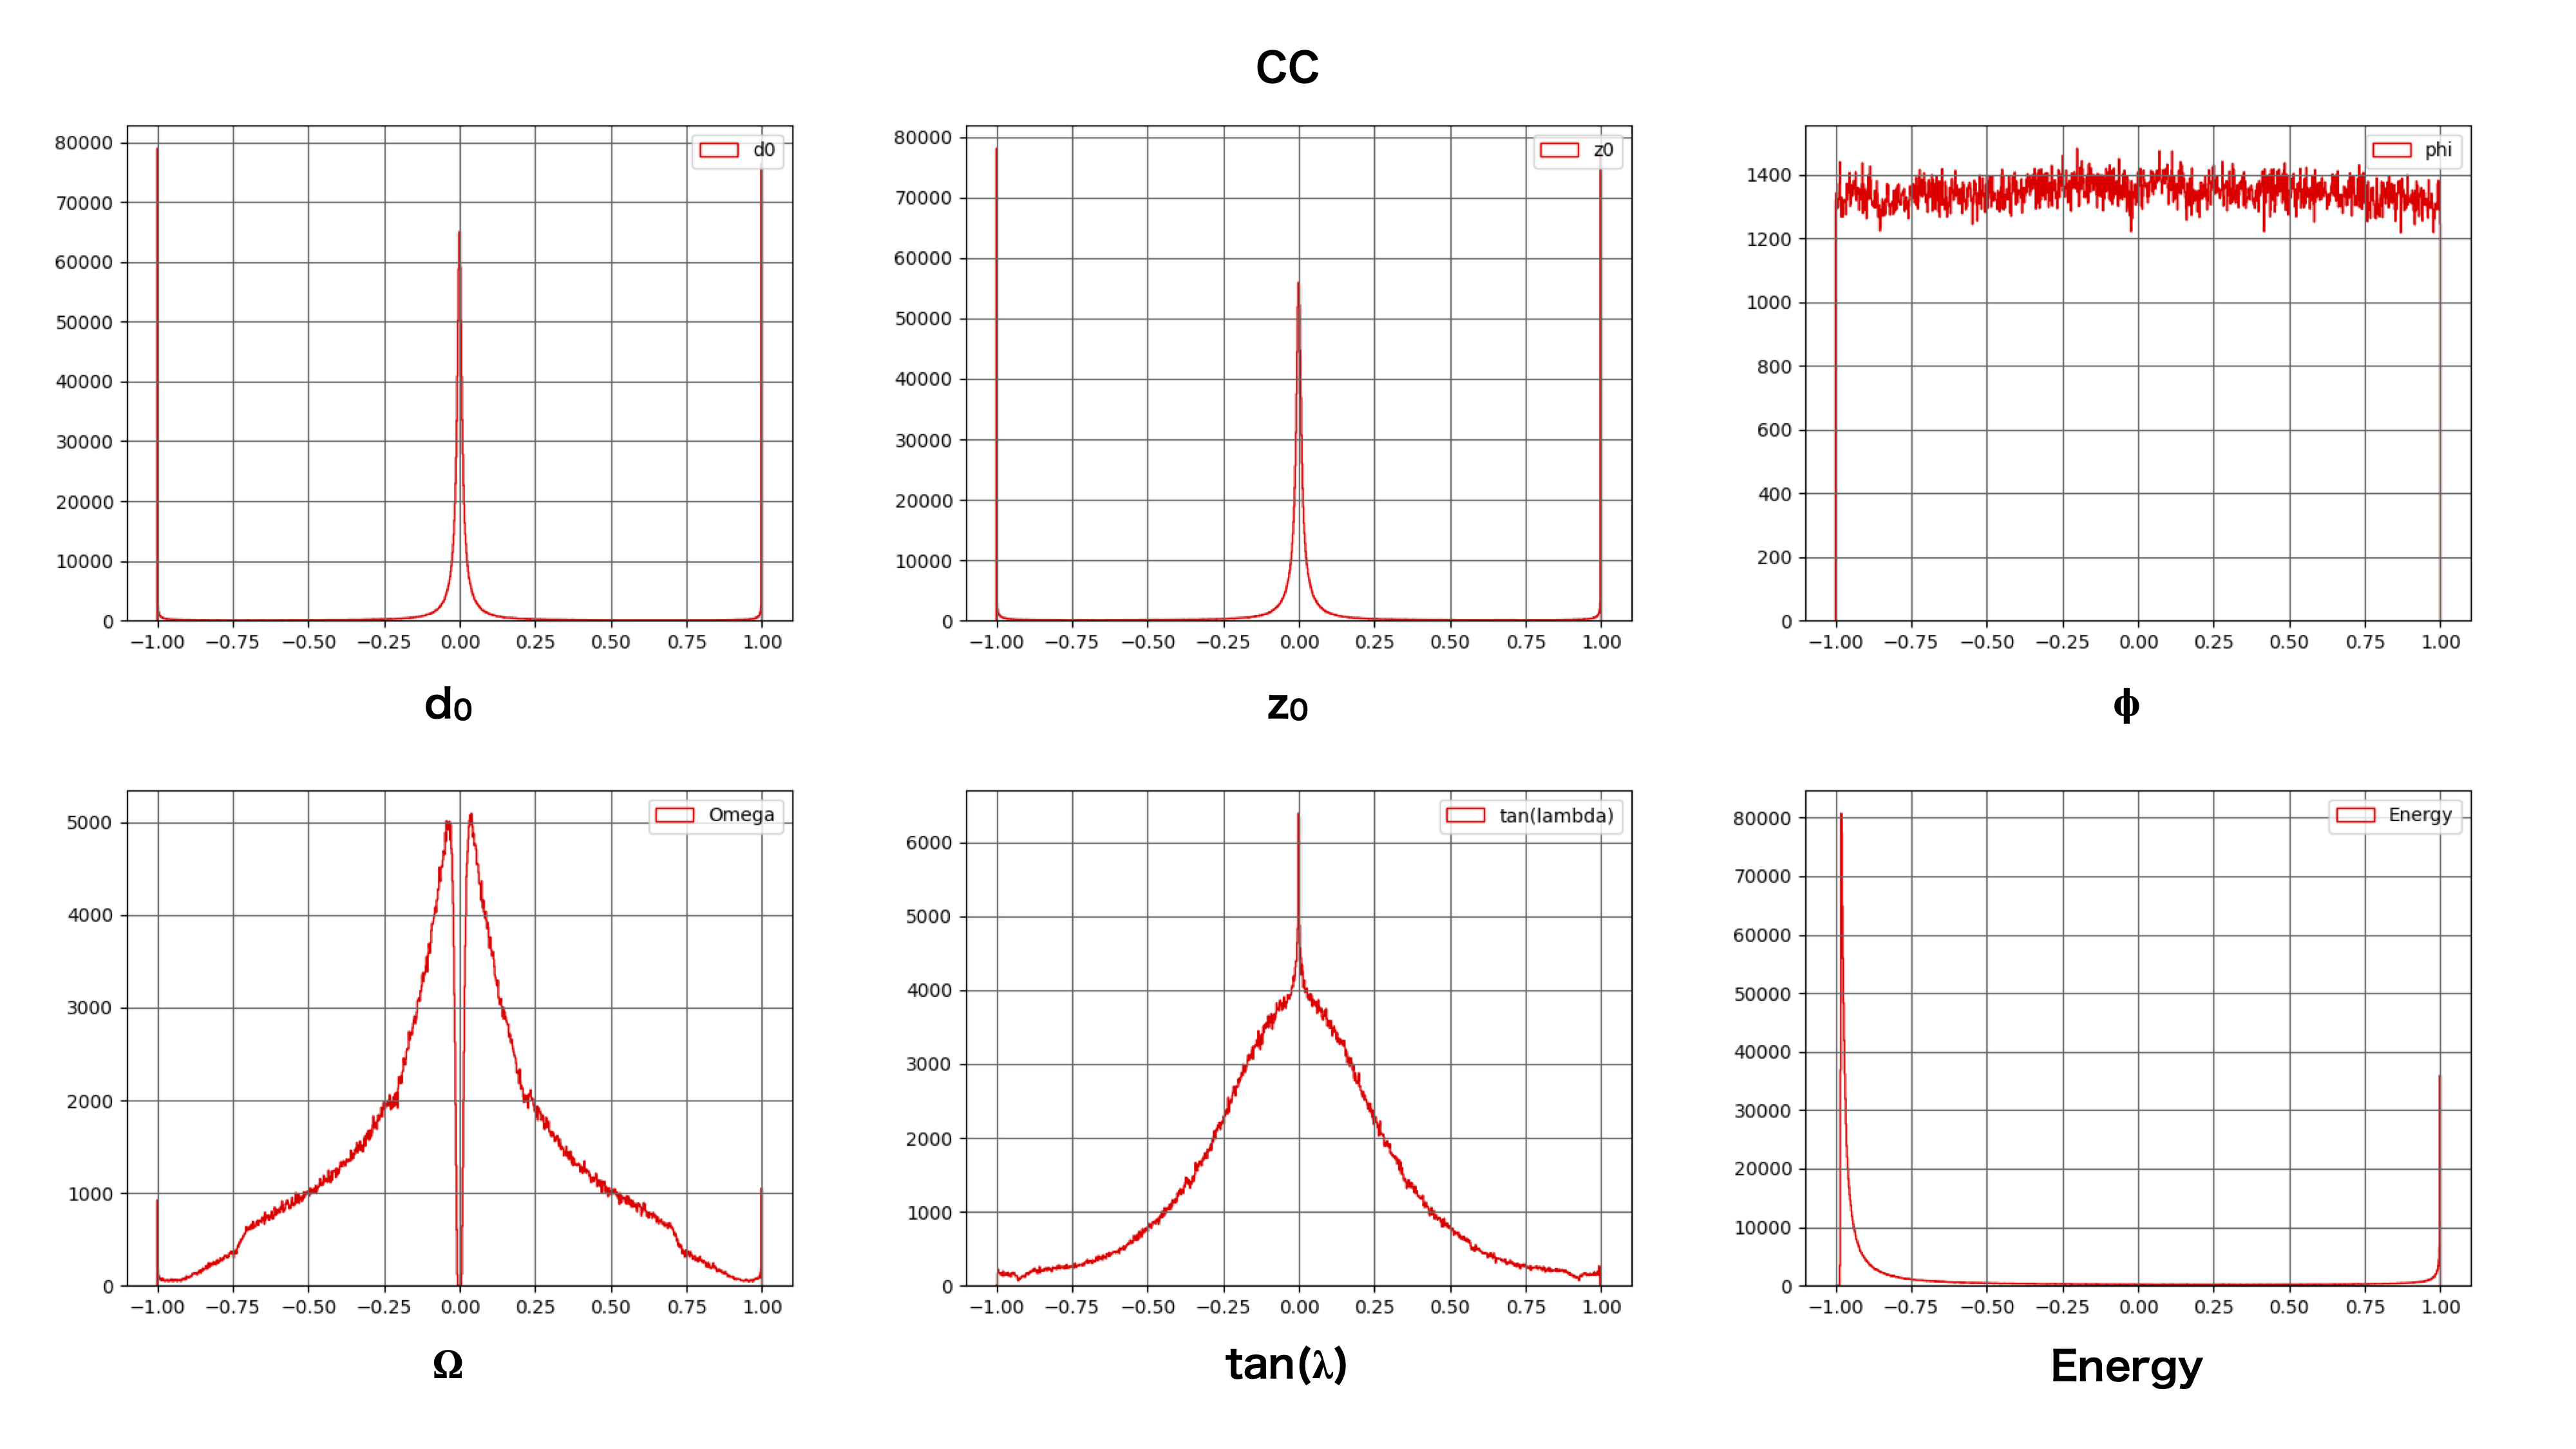
\includegraphics[width=1.0\textwidth, clip]{Figure/3Networks/3-1-2-2ReshapedVariablesCC.png}
    \subcaption{終状態$\rm c\bar{c}$での変換後の変数の分布}
    \label{3-1-2-2ReshapedVariablesCC}
   \end{minipage}
   \end{minipage}
  \caption{変数の分布の例}
  \label{3-1-2-2Variables}
 %\end{tabular}
\end{figure}

また、LCFIPlusのフィッティングで得られる$\chi^2$や崩壊点の位置についてもデータを用意した。
ここでは、事象中の二本の飛跡 (飛跡対) の全ての組み合わせについて計算を行った。
ただし、このような高次の情報を含んだ変数は基本的にはネットワークの学習に使用せず、正解ラベルの一つとして使用した。
LCFIPlusによって予想される崩壊点の位置について、ビーム衝突点からの距離を図\ref{3-1-2-3VertexPositions}に示す。
図\ref{3-1-2-3VertexPositions}のグラフは両対数グラフとして表現している為、衝突点からの距離$10^{-2}\ \mathrm{mm}$から$10^{3}\ \mathrm{mm}$のプロットとなっており、衝突点は含んでいない。
Primary VertexとSecondary Vertexの衝突点からの距離は大きく異なっているが、各フレーバーのSecondary Vertexの衝突点からの距離は殆ど離れていないことが分かる。
また、終状態$\rm c\bar{c}$と終状態$\rm b\bar{b}$では$\rm b \to c$の崩壊過程を辿るか否かの違いがある為、チャーム・フレーバーの崩壊点の位置が少し異なっている。
Othersは衝突点付近では殆ど起こらず、他の崩壊点と比較して遠い位置で崩壊している。
このように崩壊点検出において位置の再構成は非常に重要な情報を含んでおり、逆説的に位置の再構成が出来なければ崩壊点に分離は困難であると言える。

\begin{figure}[htbp]
 \centering
 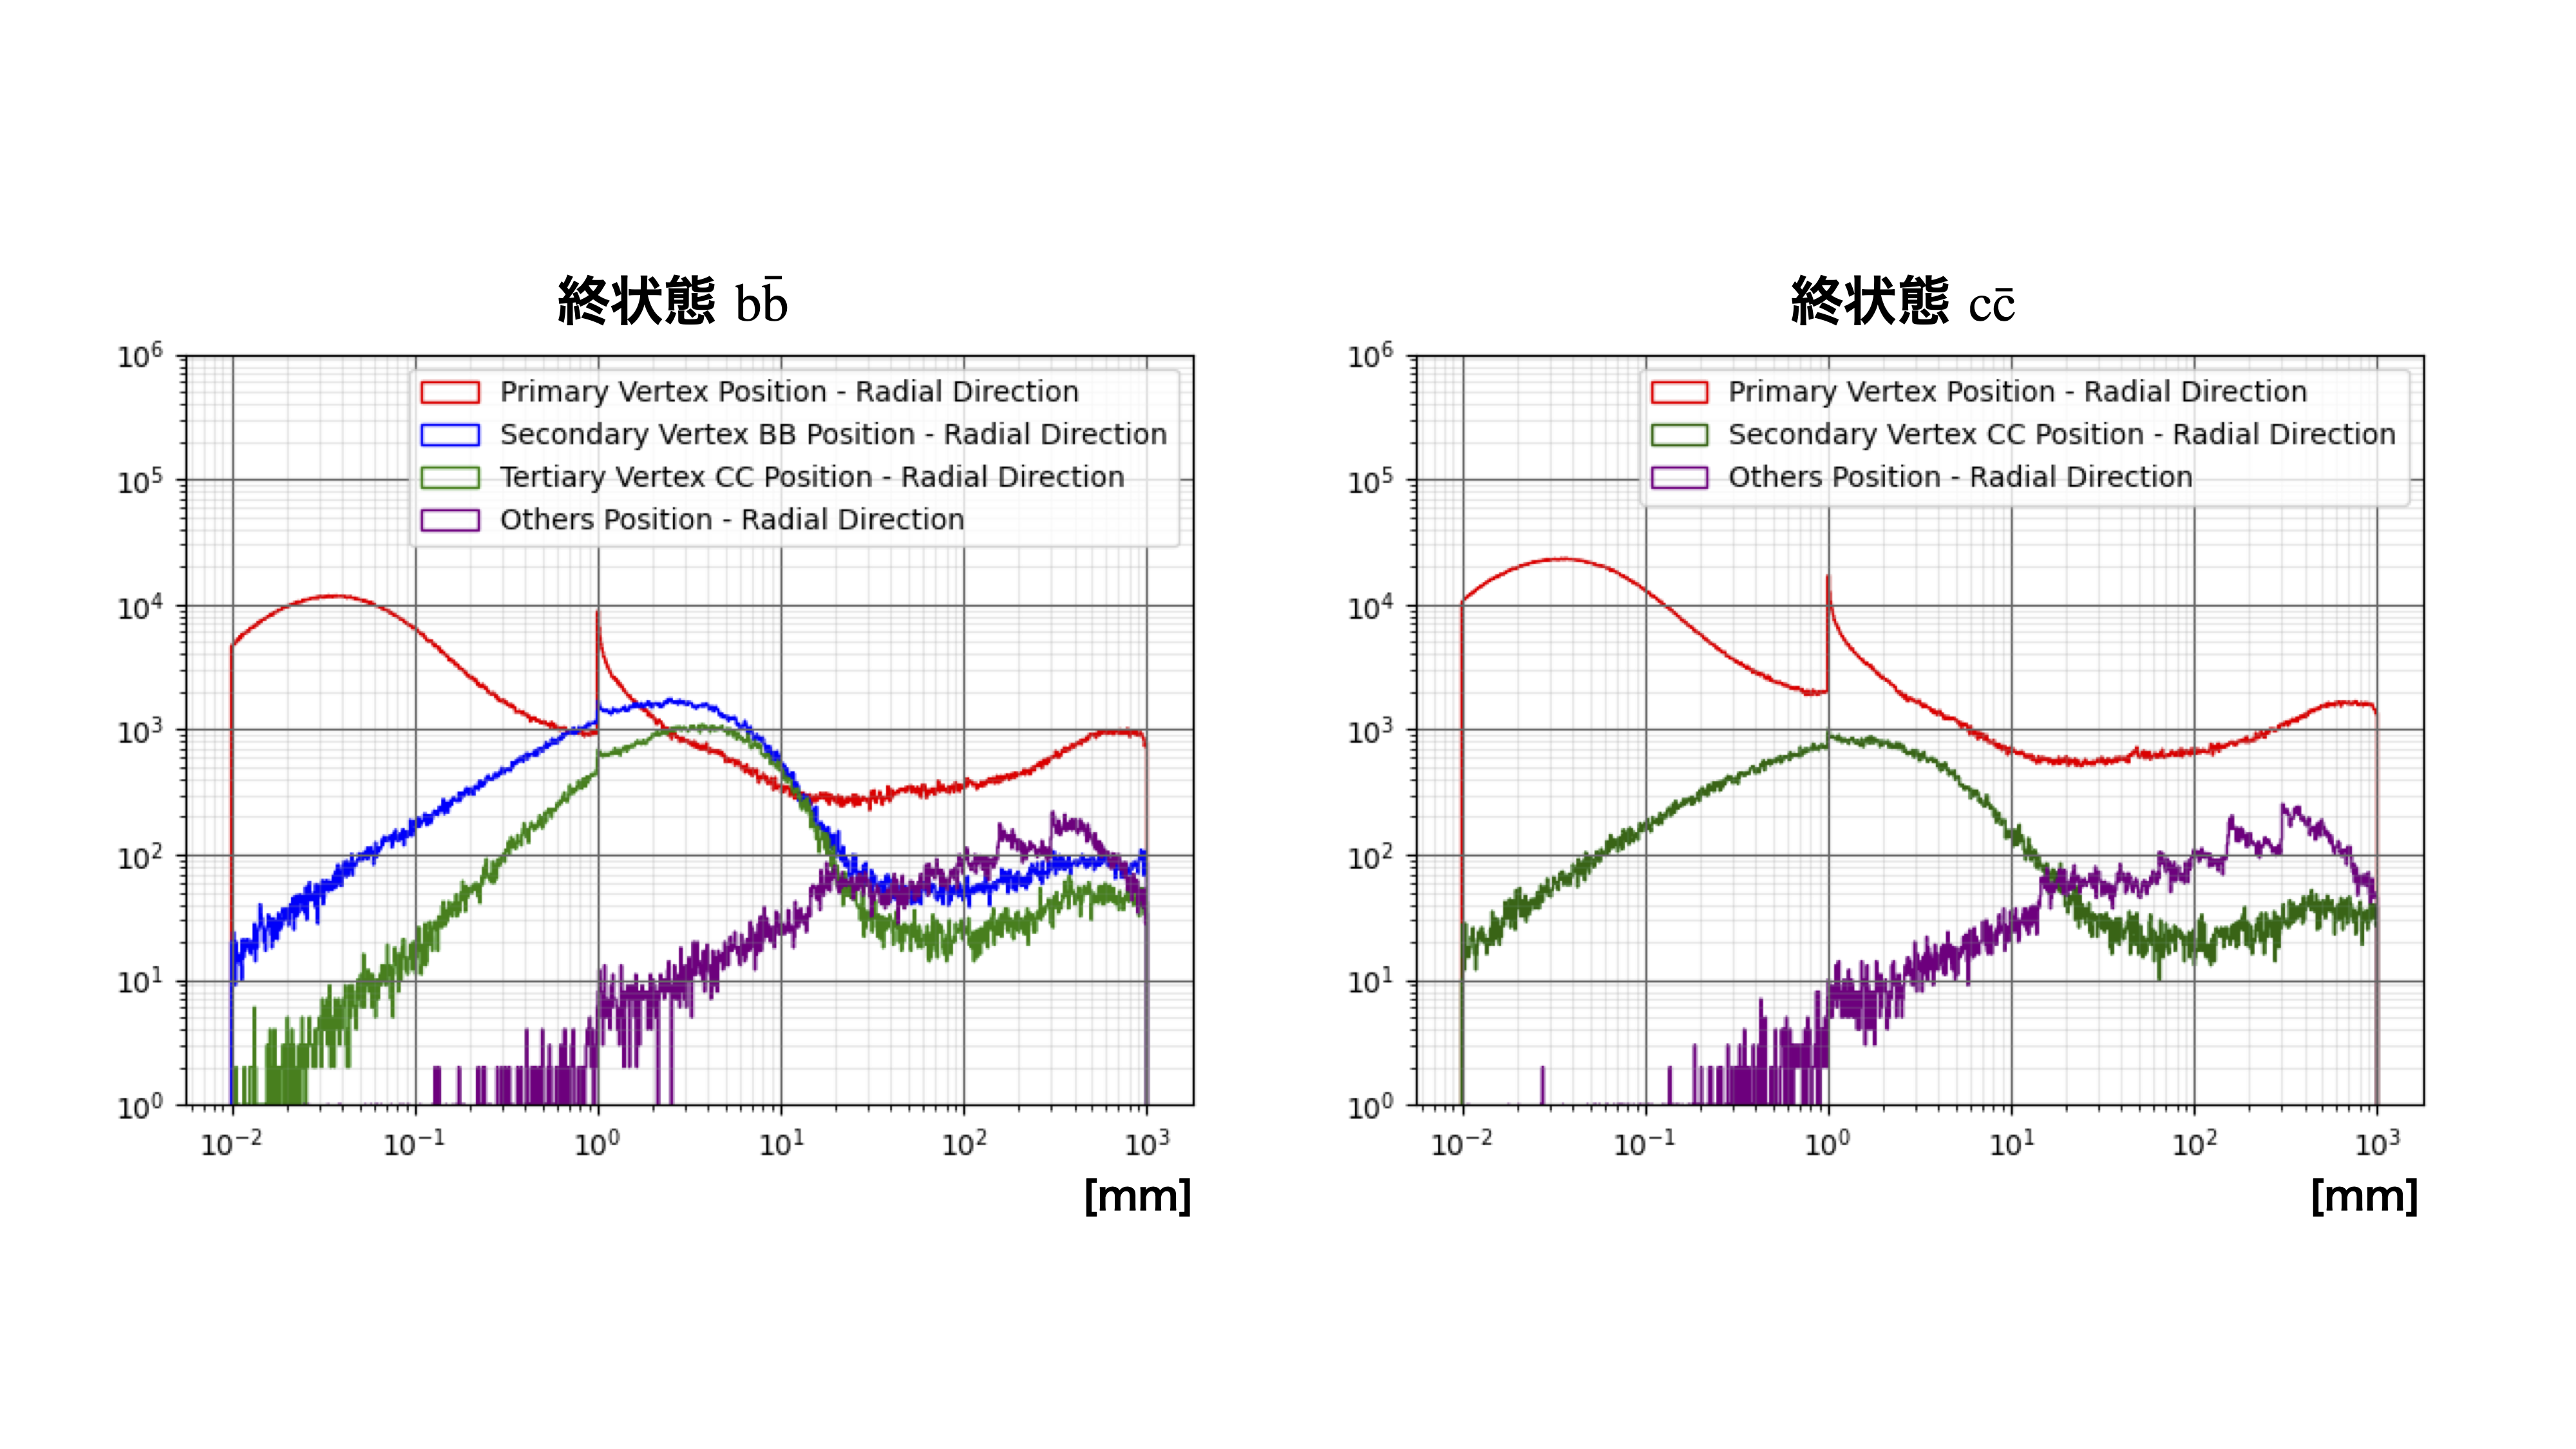
\includegraphics[trim = 50 100 50 150, width=1.0\textwidth, clip]{Figure/3Networks/3-1-2-3VertexPositions.png}
 \caption[LCFIPlusによって予想される崩壊点の位置の分布]{LCFIPlusによって予想される崩壊点の位置の分布。横軸はログスケールの衝突点からの距離である。赤線はPrimary Vertexの位置、青線はボトム・フレーバーのSecondary Vertexの位置、緑線はチャーム・フレーバーのSecondary Vertexの位置、紫線はOthersの位置を表している。これらは飛跡対についてのLCFIPlusの計算値である。}
 \label{3-1-2-3VertexPositions}
\end{figure}

$1\ \mathrm{mm}$付近のピークはLCFIPlusのフィッティングが失敗している飛跡対である。
フィッティング健全性を表す$\chi^2$との相関を見ると、図\ref{3-1-2-4VertexPositionsvsChiSquare}のように、$1\ \mathrm{mm}$付近のデータは大きな$\chi^2$値を持っていることが分かる。

\begin{figure}[htbp]
 \centering
 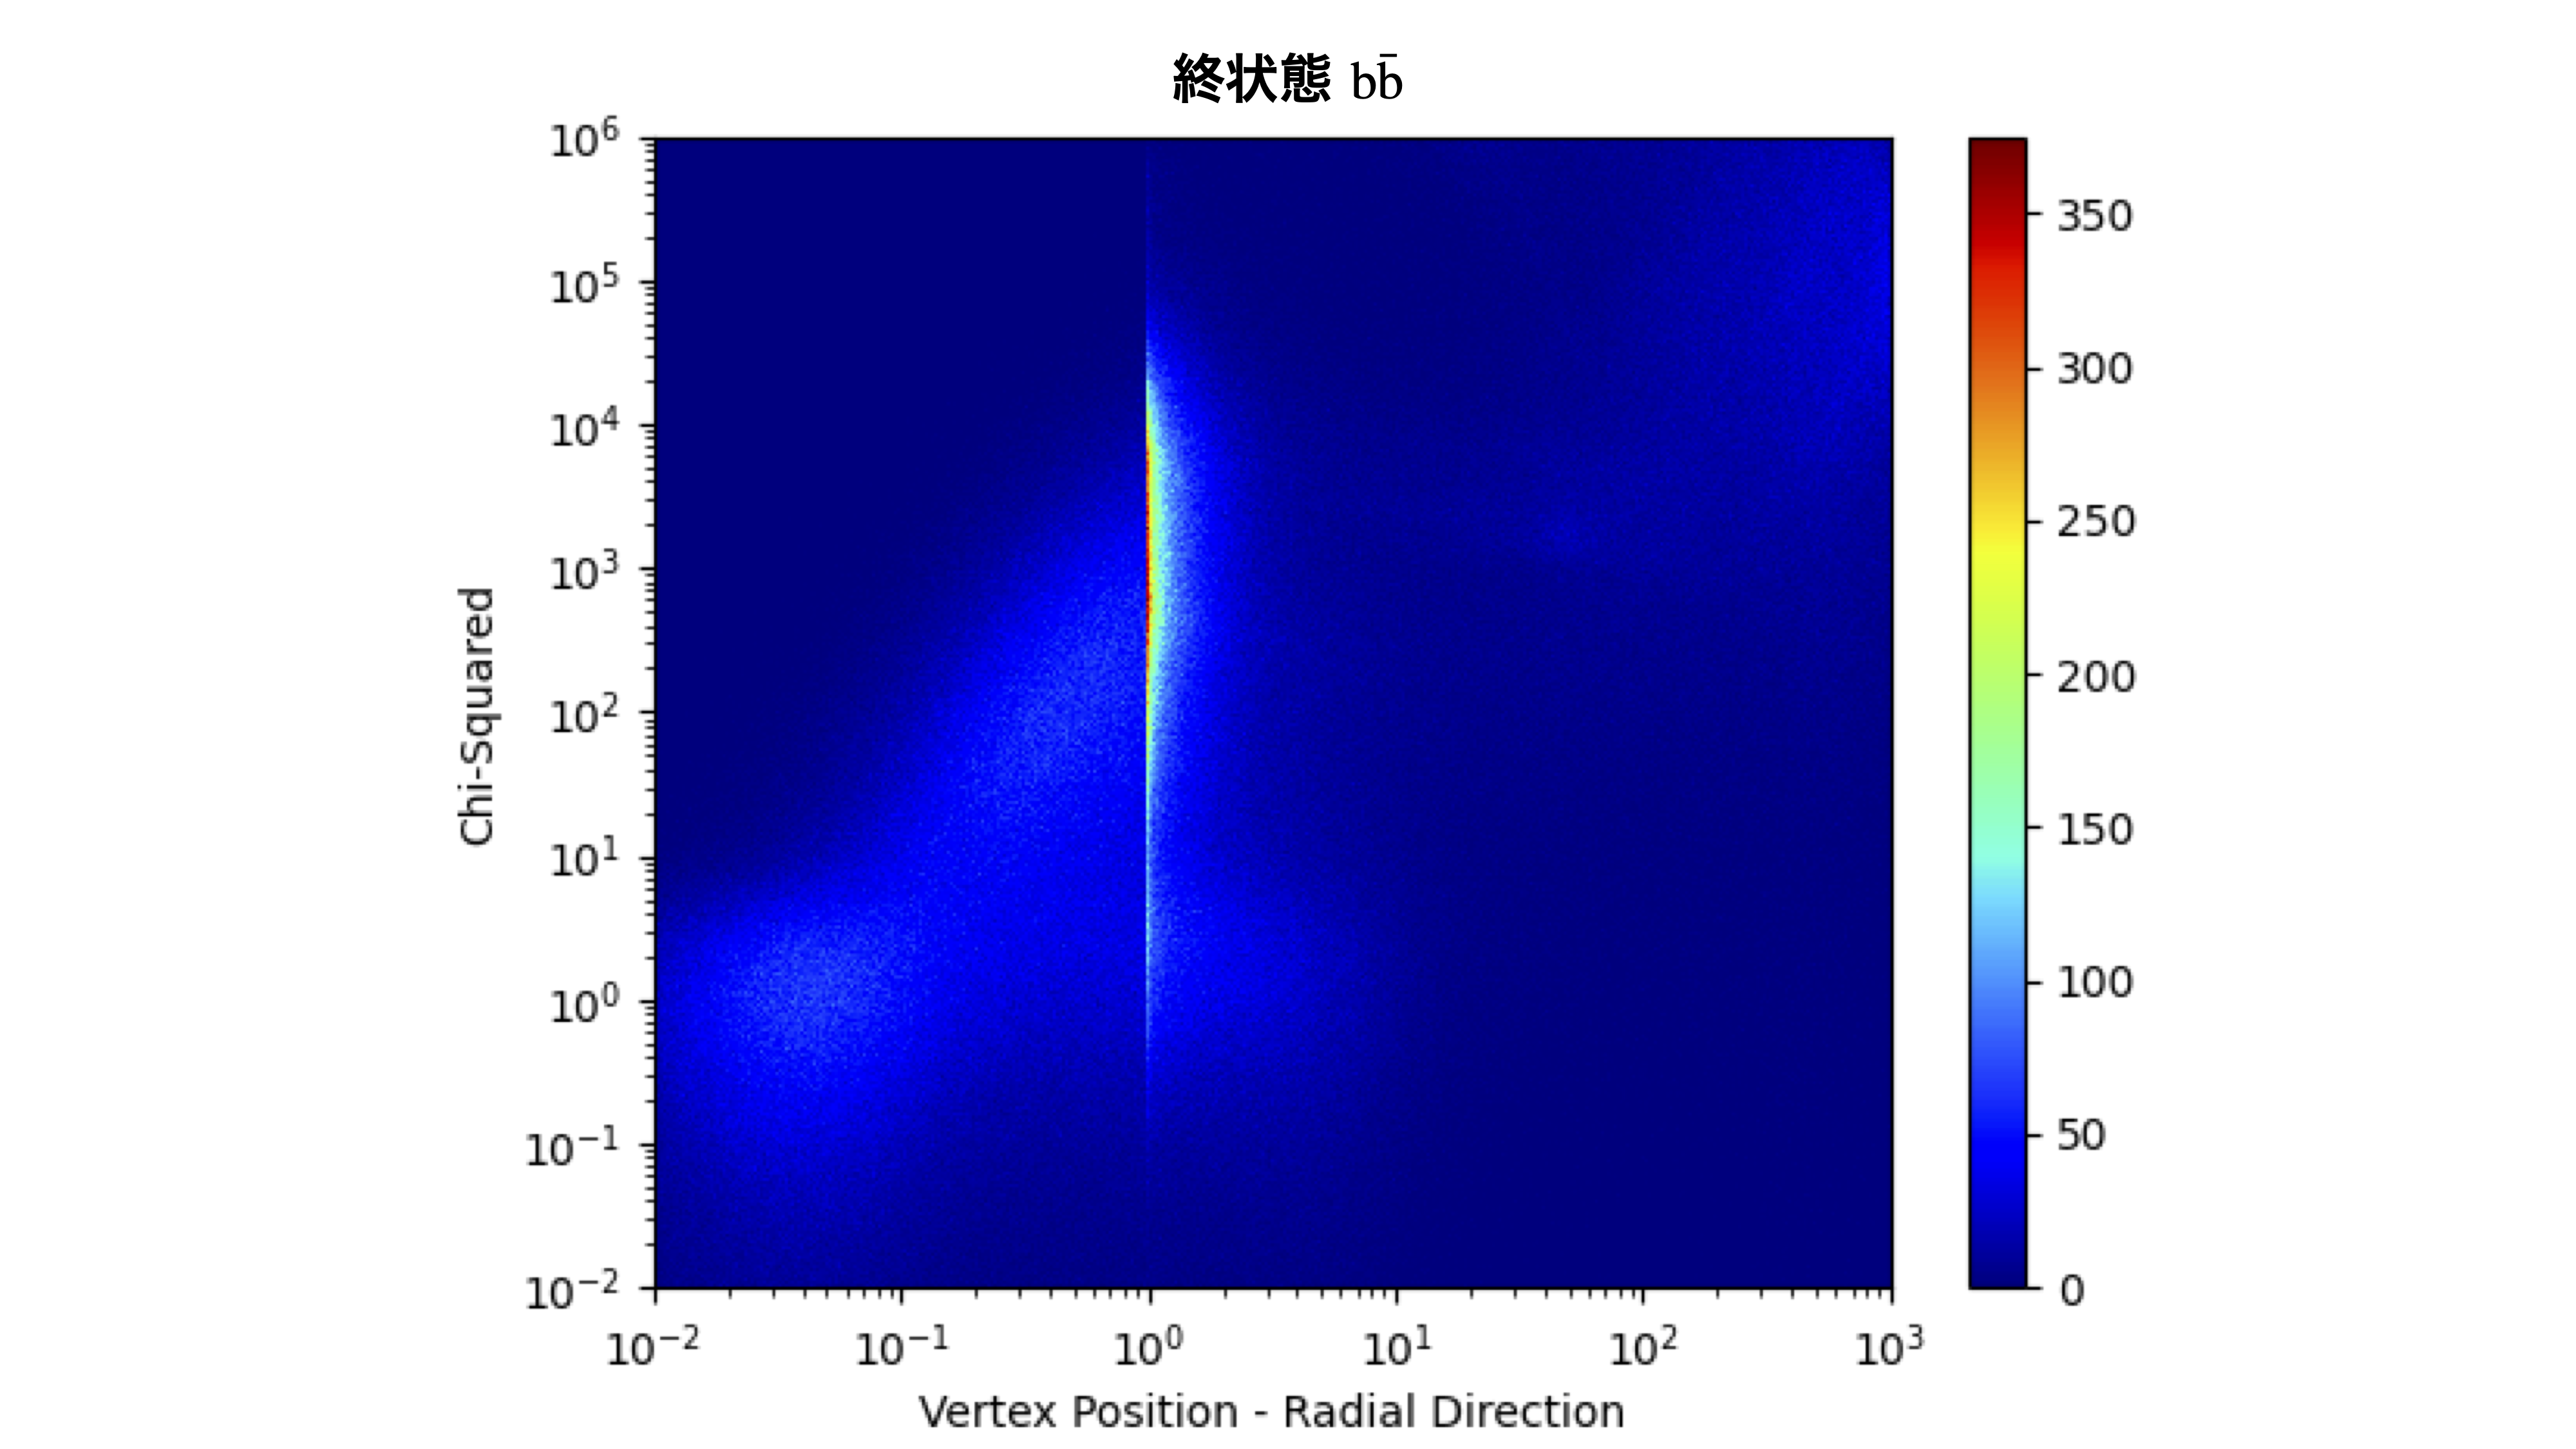
\includegraphics[width=1.0\textwidth, clip]{Figure/3Networks/3-1-2-4VertexPositionsvsChiSquare.png}
 \caption[LCFIPlusによって予想される崩壊点の位置と$\chi^2$値の相関]{LCFIPlusによって予想される崩壊点の位置と$\chi^2$値の相関。縦軸、横軸はそれぞれログスケールの$\chi^2$値、ログスケールの衝突点からの距離である。カラースケールはカウントを示しており、$1\ \mathrm{mm}$付近で非常に大きな値になっていることがわかる。}
 \label{3-1-2-4VertexPositionsvsChiSquare}
\end{figure}

\newpage
%%%%%%%%%%%%%%%%%%%%%%%%%%%%%%%%%%%%%%%%%%%%%%%%%%%%%%%%%%%%%%%%%%%%%%%%%%%%%%%%%%%%%%%%%%%%%%%%%%%%%
\section{深層学習を用いた崩壊点検出の実現} \label{Net:forVertexFinderwithDL}

深層学習は分類問題や回帰問題を解けるが、一方で基本的にはクラスタリングなど教師なし学習に対しては不向きである。
分類問題や回帰問題では訓練データから「パターン」を学び、データの持つ特徴量の空間内である種の境界を引く必要がある。
この「パターン」はあらゆるデータ内で分類可能な決まった性質を持っていなければならない。
例えば\ref{Net:Data:DataProperty}項では、同一フレーバーのSecondary Vertexが主に二つあることを解説した。
この二つのSecondary Vertexは事象内では位置の違いによって区別できるが、あらゆる事象間で不変的に一番や二番といったラベル付けできる性質を持っていない。\footnote{実際には損失関数を最小にするような順序を与えることで分離することは可能であるが本研究においては様々なSecondary Vertexが存在する為不適である。}

崩壊点検出アルゴリズムの目的は同一フレーバー内の複数のSecondary Vertexを含む崩壊点を探索する事である。
このような問題は一般にクラスタリングを用いて解くことが多いが、本研究で使用するデータは図\ref{3-1-1-2TracksandVertices}で示したように事象内に含まれる飛跡の本数や崩壊点の個数も異なっているという性質を持っている。
これはクラスター数やクラスターに含まれる要素数が常に変わってしまうということを意味しており、崩壊点検出をクラスタリングで行うことは不適であると判断した。

以上を踏まえた上で私は次の二つのネットワークを用いた崩壊点検出を提案する。

\begin{enumerate}
 \item 飛跡対についてのネットワーク
 \begin{itemize}
  \item 用途 : 崩壊点のタネの探索
  \item 入力 : 事象内のあらゆる飛跡対 (二本の飛跡の全ての組み合わせ)
  \item 出力 : 飛跡対の属する崩壊点の種類・崩壊点の位置
 \end{itemize}
 \item 任意の数の飛跡についてのネットワーク
 \begin{itemize}
  \item 用途 : 崩壊点の生成
  \item 入力 : 崩壊点のタネ・事象内の全ての飛跡
  \item 出力 : 事象内のそれぞれの飛跡が崩壊点のタネに結合しているか否か
 \end{itemize}
\end{enumerate}

飛跡対についてのネットワークは崩壊点のタネとなる飛跡対を探索するネットワークである。
したがって、このネットワーク単体では崩壊点を形成することはできない。
そこで、私は崩壊点の生成を行う、もう一つのネットワークを構築した。
崩壊点の生成を行うネットワークは二本以上の飛跡を取り扱う必要があるが、三本、四本、五本の飛跡を取り扱えるネットワークをそれぞれ構築することはネットワークや組み合わせの数を考える上で適切ではない。
よって不定の数の飛跡を再帰的に処理するネットワーク構造として、リカレントニューラルネットワークを使用した。
任意の数の飛跡についてのネットワークは崩壊点のタネをリカレントニューラルネットワークの初期状態として、そこに飛跡を一本ずつ加え崩壊点の生成を行うネットワークである。
本研究は以上の二つのネットワークを用いることで崩壊点検出を実現した。
構造や学習についての、より詳細な個々のネットワークの解説は、後の\ref{Net:PairModel}節や\ref{Net:VertexLSTM}節で述べる。

本研究のネットワークはTensorflow/Kerasフレームワークを用いて構築・学習を行なった。
また、学習に際しては計算機として、弊研究室サーバーの"NVIDIA TITAN RTX"や九州大学情報基盤研究開発センター研究用計算機システムの一般利用を使用した。
詳細なソフトウェア・ハードウェアの環境を表\ref{SoftwareHardwareEnvironments}に示す。

\begin{table}[htb]
 \centering
 \small
  \begin{tabular}{l c} \hline
    ソフトウェア&\\\hline\hline
    Python & $3.6.8$\\
    Tensorflow & $2.1.0$\\
    Keras & $2.3.1$\\\hline
    ハードウェア &\\\hline\hline
    CPU& AMD EPYC 7402P 24-Core Processor 48個\\
    メモリ & $263694036\ \mathrm{kB}$\\
    GPU & NVIDIA Corporation TU102 [TITAN RTX] 2個\\\hline
  \end{tabular}
  \caption{ソフトウェア・ハードウェアの環境}
  \label{SoftwareHardwareEnvironments}
\end{table}


%%%%%%%%%%%%%%%%%%%%%%%%%%%%%%%%%%%%%%%%%%%%%%%%%%%%%%%%%%%%%%%%%%%%%%%%%%%%%%%%%%%%%%%%%%%%%%%%%%%%%
\section{飛跡対についてのネットワーク} \label{Net:PairModel}

ここでは\ref{Net:forVertexFinderwithDL}節で紹介した二つのネットワークの内、飛跡対についてのネットワークに関して述べる。
主にネットワークの構造に関しては\ref{Net:PM:StructureofPM}項で、学習に関しては\ref{Net:PM:TrainingandStrategyofPM}項で解説する。
また、そのようにして構築、訓練されたネットワーク単体についての性能と評価に関しては、\ref{Net:PM:PerformanceofPM}項で述べることとする。

飛跡対についてのネットワークは、崩壊点のタネを探索するためのネットワークであり、入力は二本の飛跡についての情報、出力は飛跡対についての崩壊点の種類や位置である。
この崩壊点の種類を考える上で\ref{Net:Data:DataProperty}項で述べた、終状態によって生じる崩壊点の種類の違いを考慮しなければならない。
例えば、終状態$\rm b\bar{b}$の場合は$\rm b \to c$という崩壊過程を辿り、ボトム・フレーバーのSecondary Vertexとチャーム・フレーバーのTertiary Vertexが生じ、終状態$\rm c\bar{c}$の場合はチャーム・フレーバーのSecondary Vertexのみが生じる。
また両方の終状態について、これら以外の崩壊点であるOthers\footnote{タウ粒子の崩壊やストレンジ ($\rm s$) ・フレーバーのハドロンの崩壊、光子変換}を考える必要がある。
更に終状態$\rm b\bar{b}$の場合について、ボトム・フレーバーのSecondary Vertexからの飛跡とそこから生じたチャーム・フレーバーのTertiary Vertexからの飛跡を一本ずつ含んだ飛跡対を準崩壊点として定義する。 (図\ref{3-3-0-1SecondaryVertexBC}) 

以上より、飛跡対についての崩壊点の種類は"非結合な飛跡対 (Not Connected, NC)"、"Primary Vertex (PV)"、"チャーム・フレーバーのSecondary Vertex (SVCC)"、"ボトム・フレーバーのSecondary Vertex (SVBB)"、"チャーム・フレーバーのTertiary Vertex (TVCC)"、"終状態$\rm b\bar{b}$での準崩壊点 (SVBC)"、"これら以外の崩壊点 (Others)"の計$7$つとなる。

\begin{figure}[htbp]
 \centering
 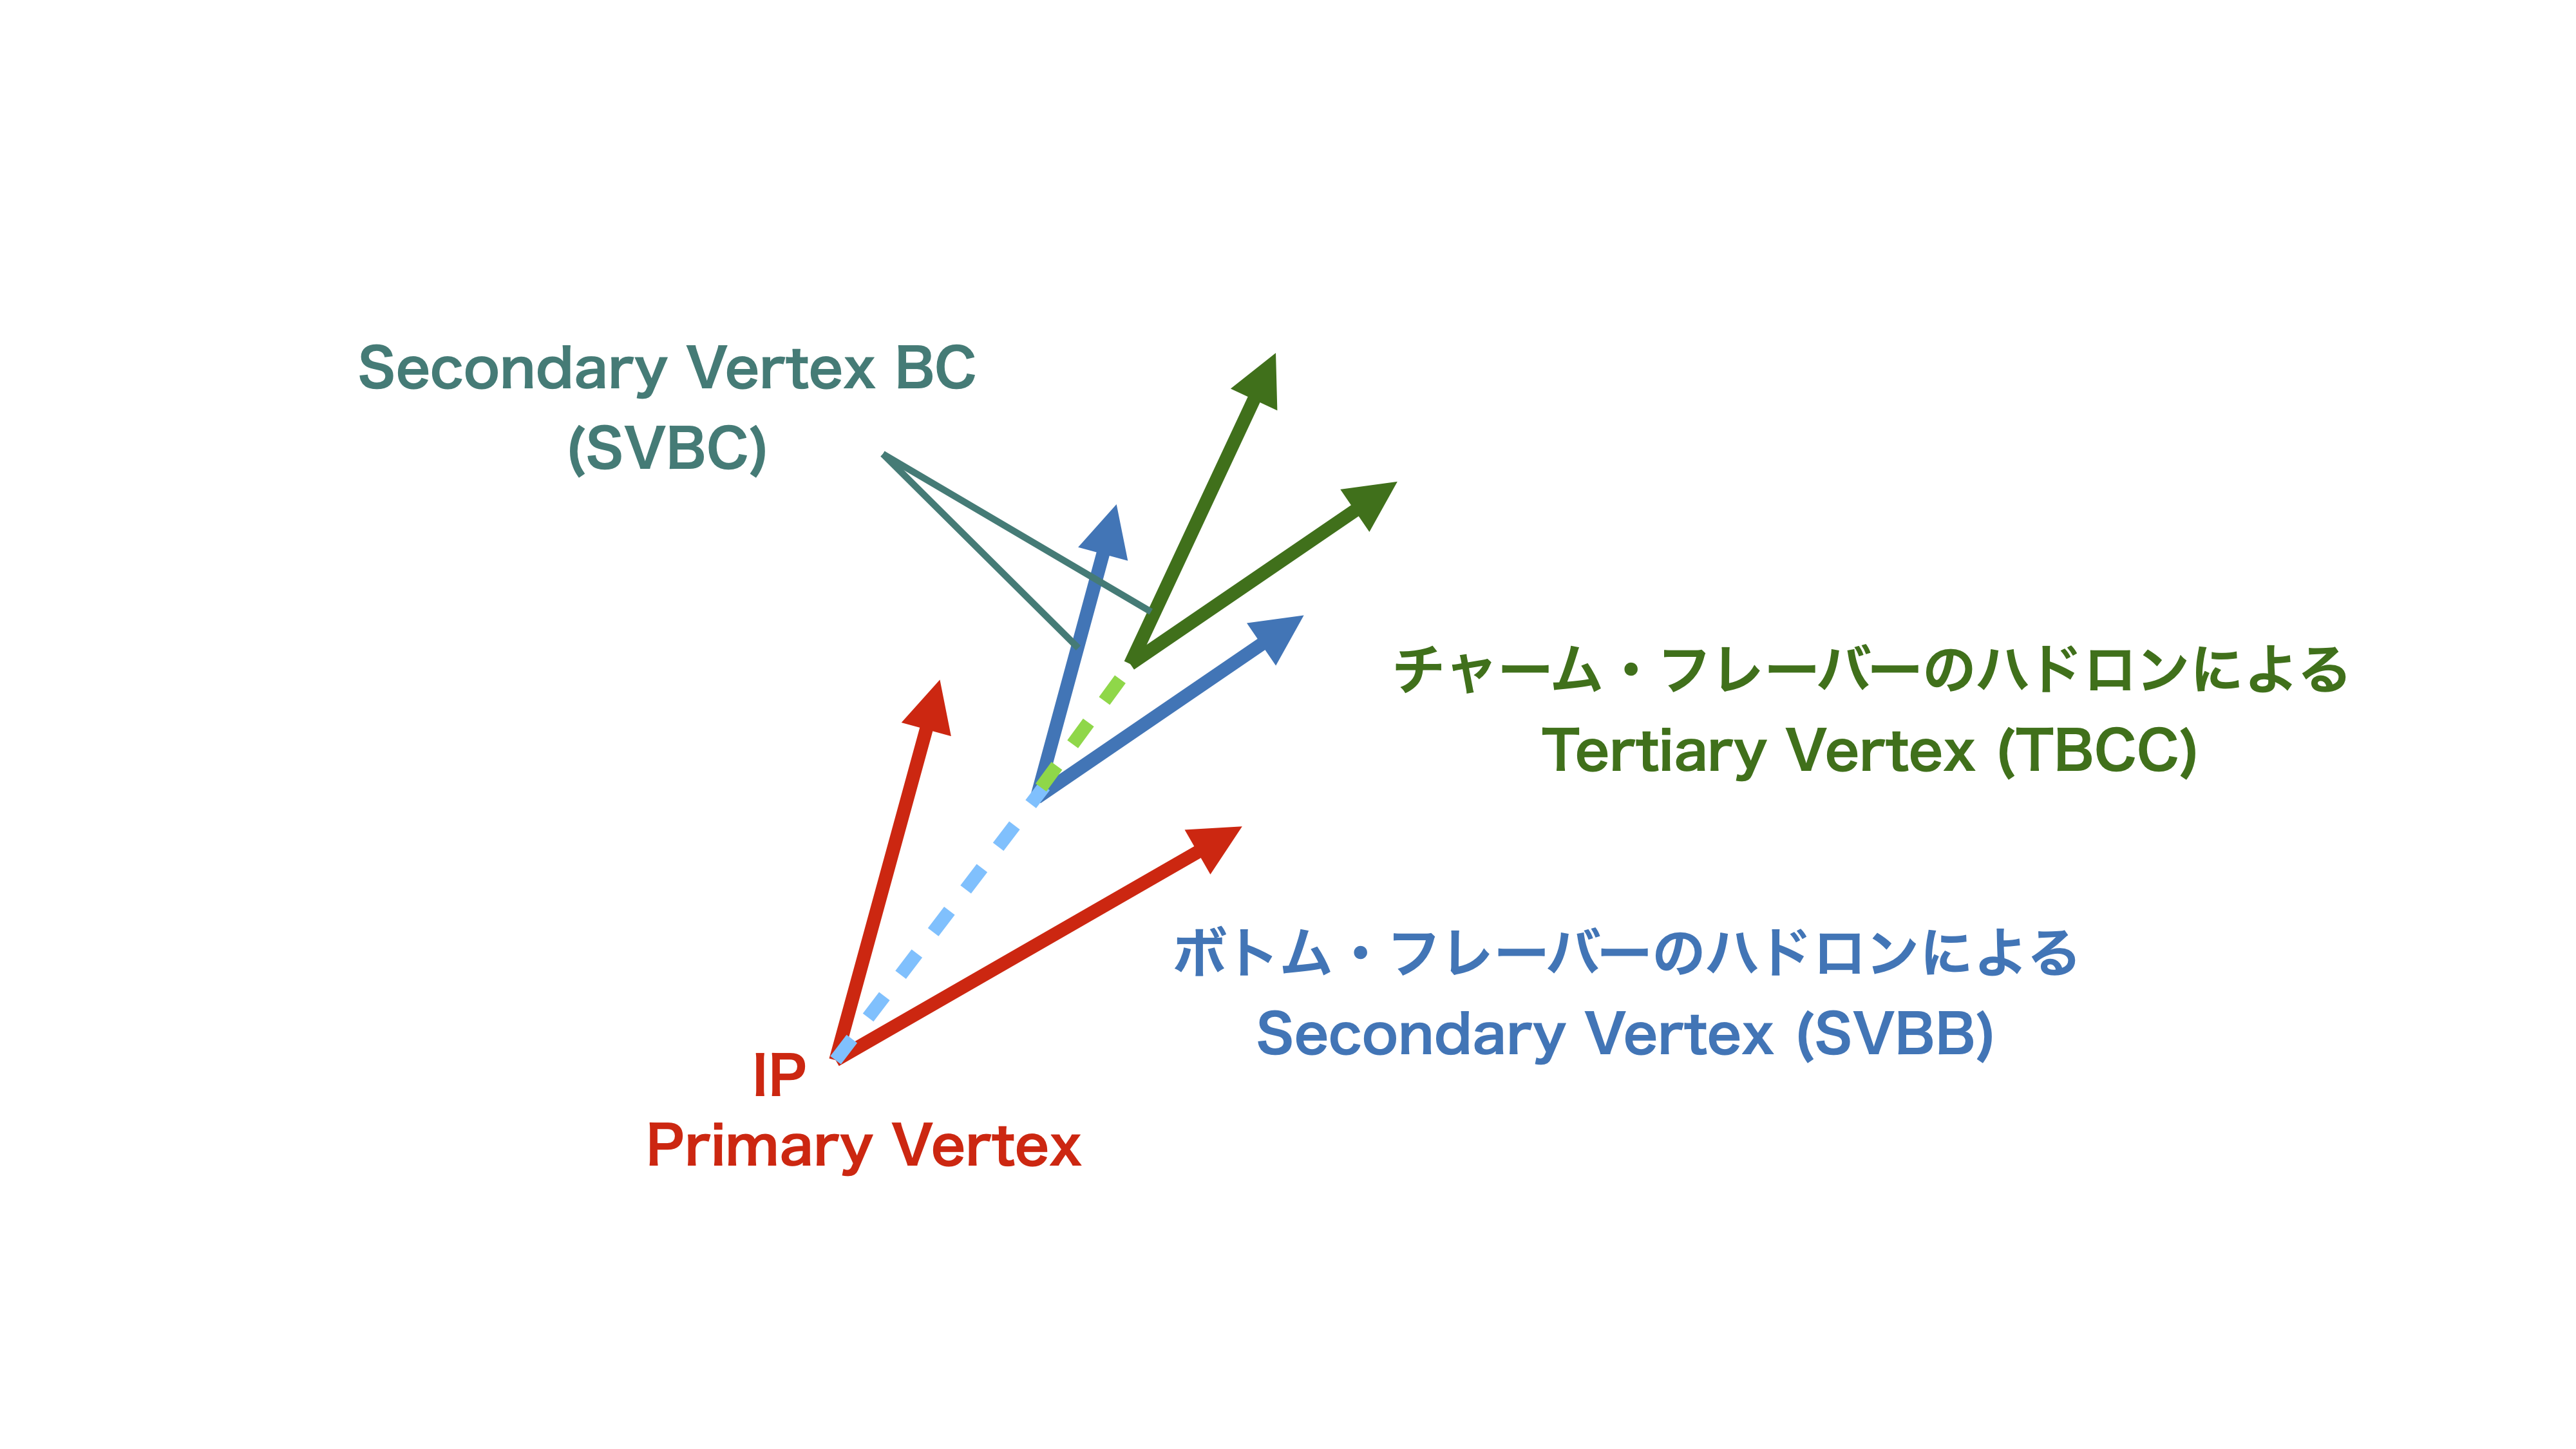
\includegraphics[trim = 200 150 200 150, width=0.9\textwidth, clip]{Figure/3Networks/3-3-0-1SecondaryVertexBC.png}
 \caption{終状態$\rm b\bar{b}$での崩壊点}
 \label{3-3-0-1SecondaryVertexBC}
\end{figure}

崩壊点の位置についての訓練データを作成するに当たって、正解ラベルとして図\ref{3-1-2-3VertexPositions}のLCFIPlusのフィッティングで得られる計算値を用いた。
こちらは回帰によって値を再現する。


%%%%%%%%%%%%%%%%%%%%%%%%%%%%%%%%%%%%%%%%%%%%%%%%%%%%%%%%%%%%%%%%%%%%%%%%
\subsection{ネットワークの構造} \label{Net:PM:StructureofPM}

飛跡対についてのネットワークとして非常にシンプルなフィードフォーワード構造を使用した。
ネットワークの概略図を図\ref{3-3-1-1PairModel}に示す。

\begin{figure}[htbp]
 \centering
 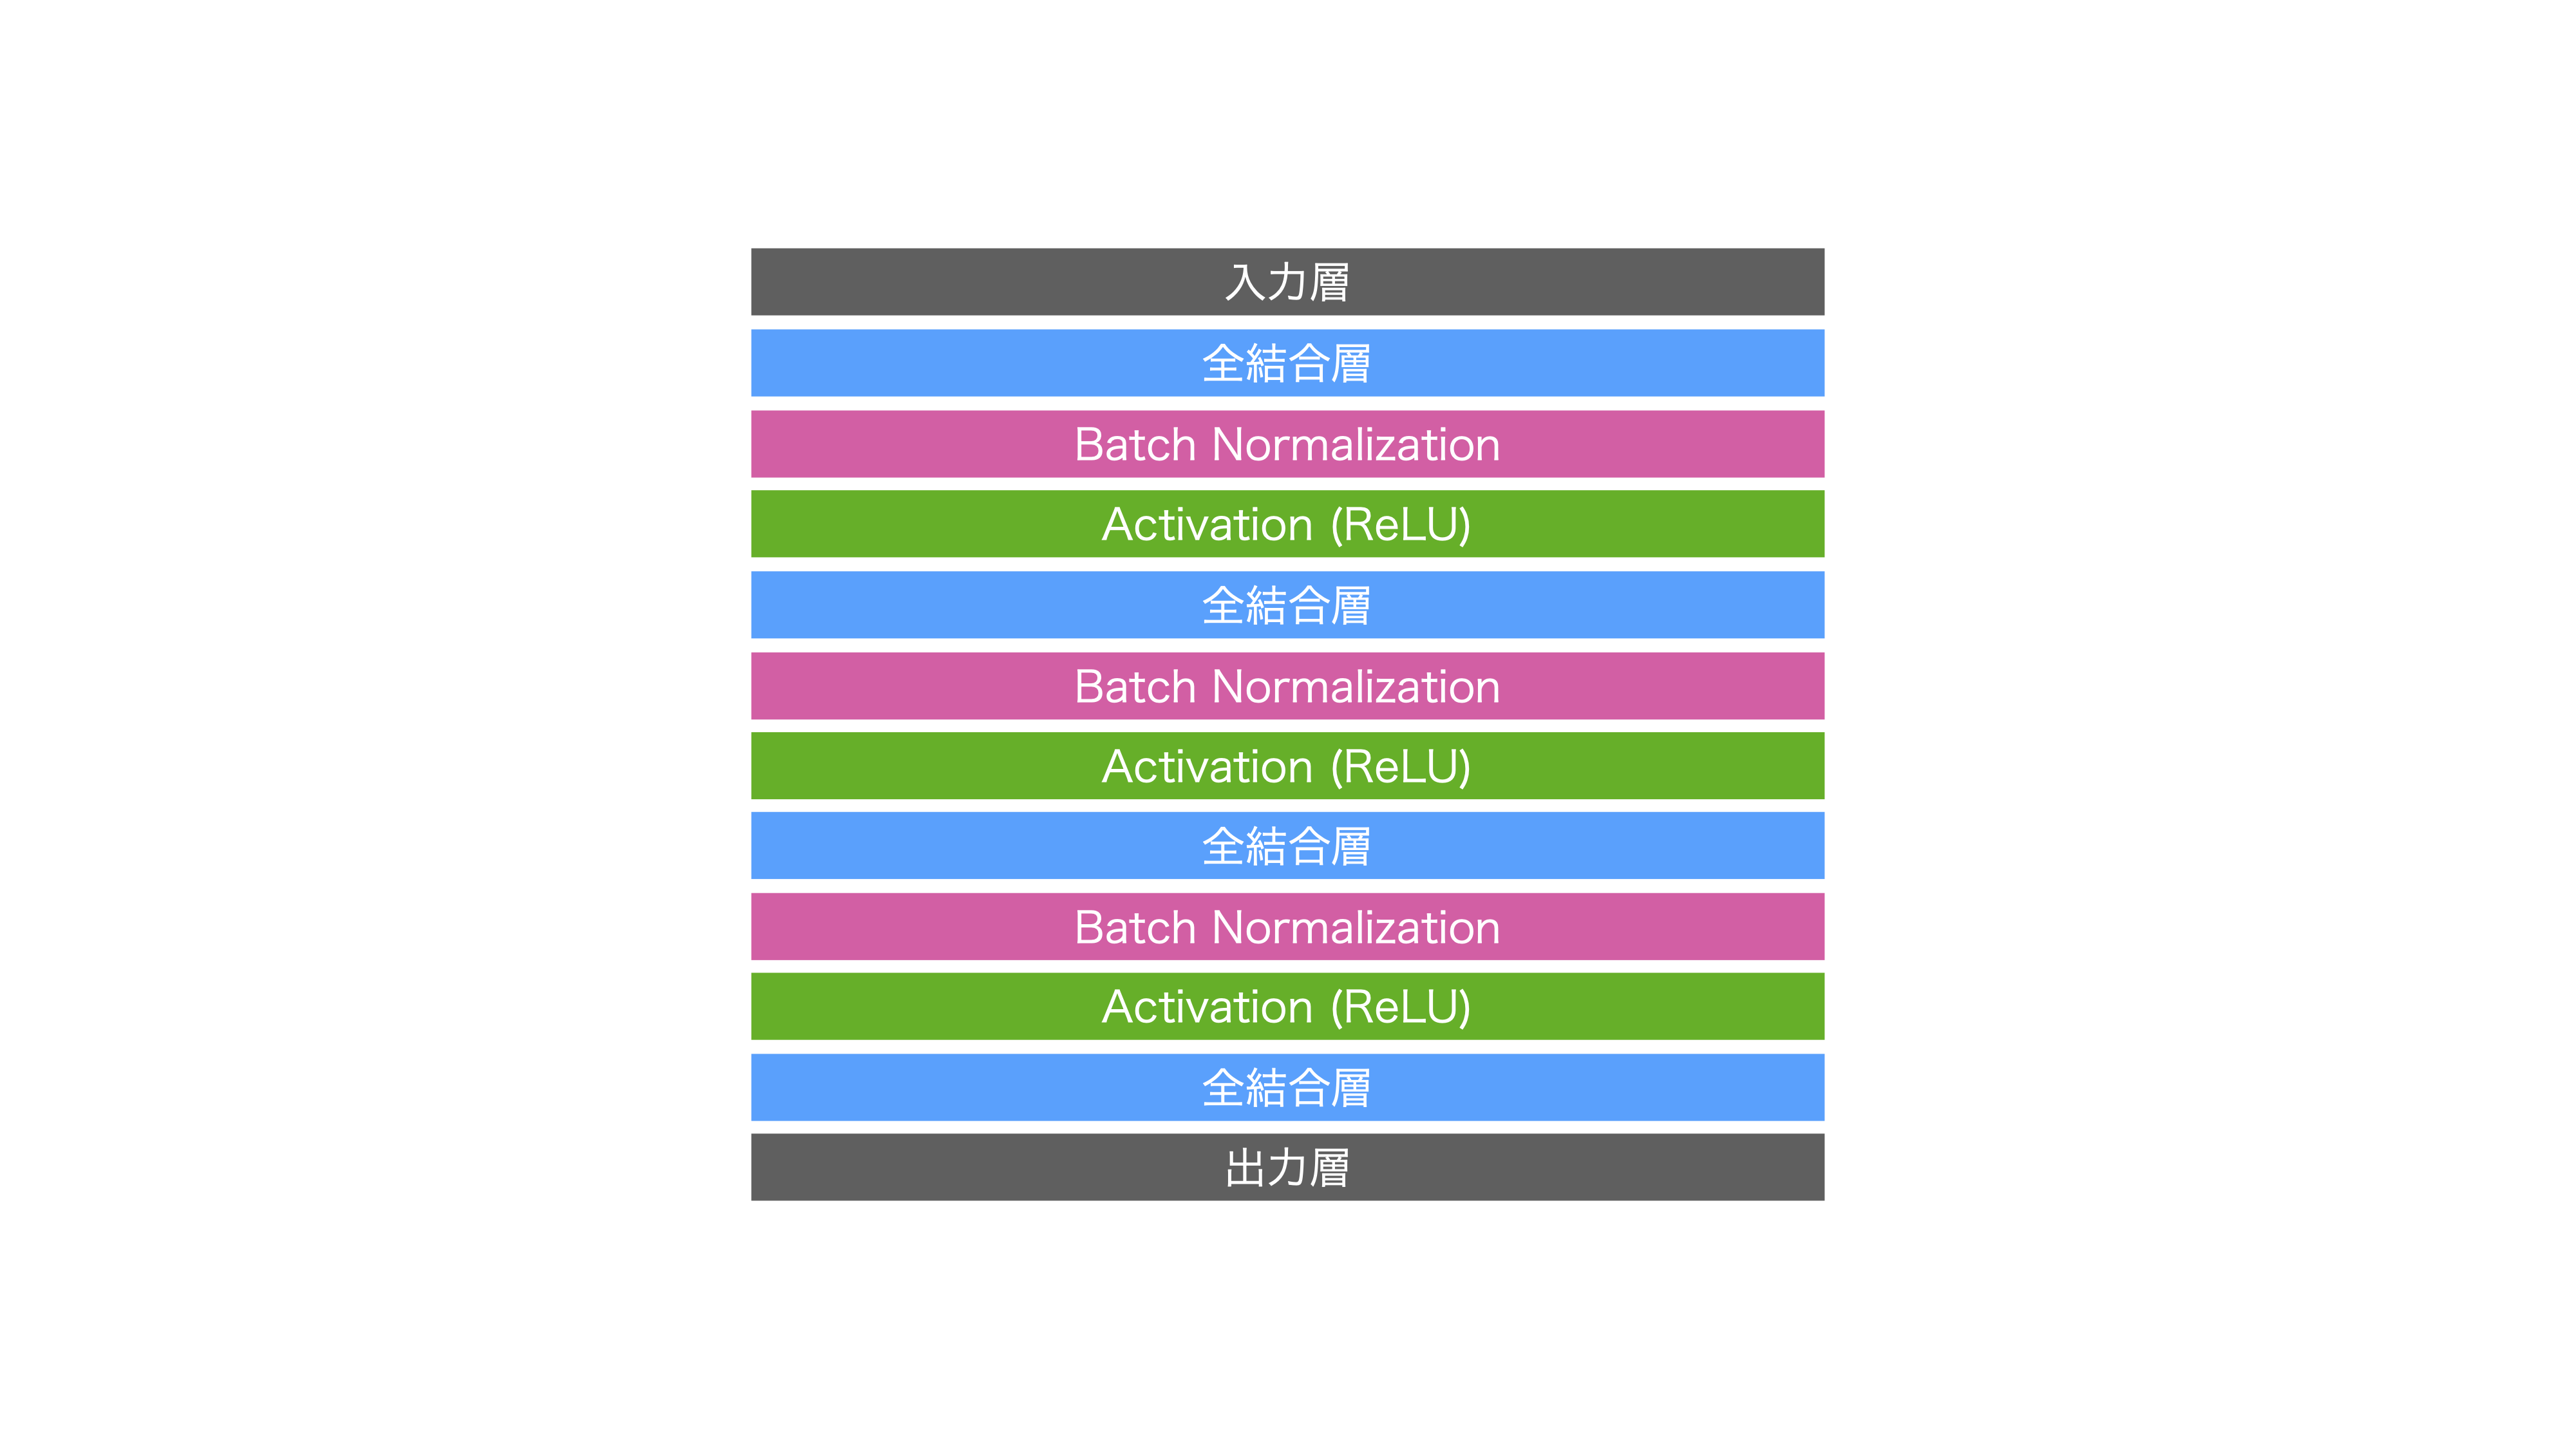
\includegraphics[trim = 200 50 200 50, width=0.9\textwidth, clip]{Figure/3Networks/3-3-1-1PairModel.png}
 \caption[飛跡対についてのネットワークの概略図]{飛跡対についてのネットワークの概略図。全結合層・Batch Normalization・活性化関数 (ReLU) を三回重ねている。その後、分類問題の為の全結合層と回帰問題の為の全結合層の二つに分離させ、それぞれで出力を行う。}
 \label{3-3-1-1PairModel}
\end{figure}

前述したように出力は、7クラス分類と回帰1つである。
出力の直前の全結合層で分類問題と回帰問題に分離させた。
また、過学習 (Over fitting) を避ける為、Batch Normalization\cite{BatchNormalizationpaper}を全結合層の後に配置した。
過学習とは、ネットワークが過度に訓練データに適合してしまい、検証データやテストデータへの汎化性能が悪化してしまう、教師あり学習の問題の一つである。
また勾配消失への対策として、活性化関数は全てReLU関数を使用した。


%%%%%%%%%%%%%%%%%%%%%%%%%%%%%%%%%%%%%%%%%%%%%%%%%%%%%%%%%%%%%%%%%%%%%%%%
\subsection{ネットワークの学習と戦略} \label{Net:PM:TrainingandStrategyofPM}

訓練データは事象中の全ての飛跡対の組み合わせを考える。
よって入力変数は飛跡二本分であるので合計$44$個である。
ここで次の二つの事柄に注意しなくてはならない。

\begin{itemize}
 \item 分類クラスは二つの終状態$\rm b\bar{b}$と$\rm c\bar{c}$を足し合わせたものである
 \item 分類クラスのデータ数の比がNCやPVが支配的な不均衡データ (Imbalanced Data) となる
\end{itemize}

各終状態での分類クラスのデータ数の比を図\ref{3-3-2-1ImbalancedData}に示す。

\begin{figure}[htbp]
 \centering
 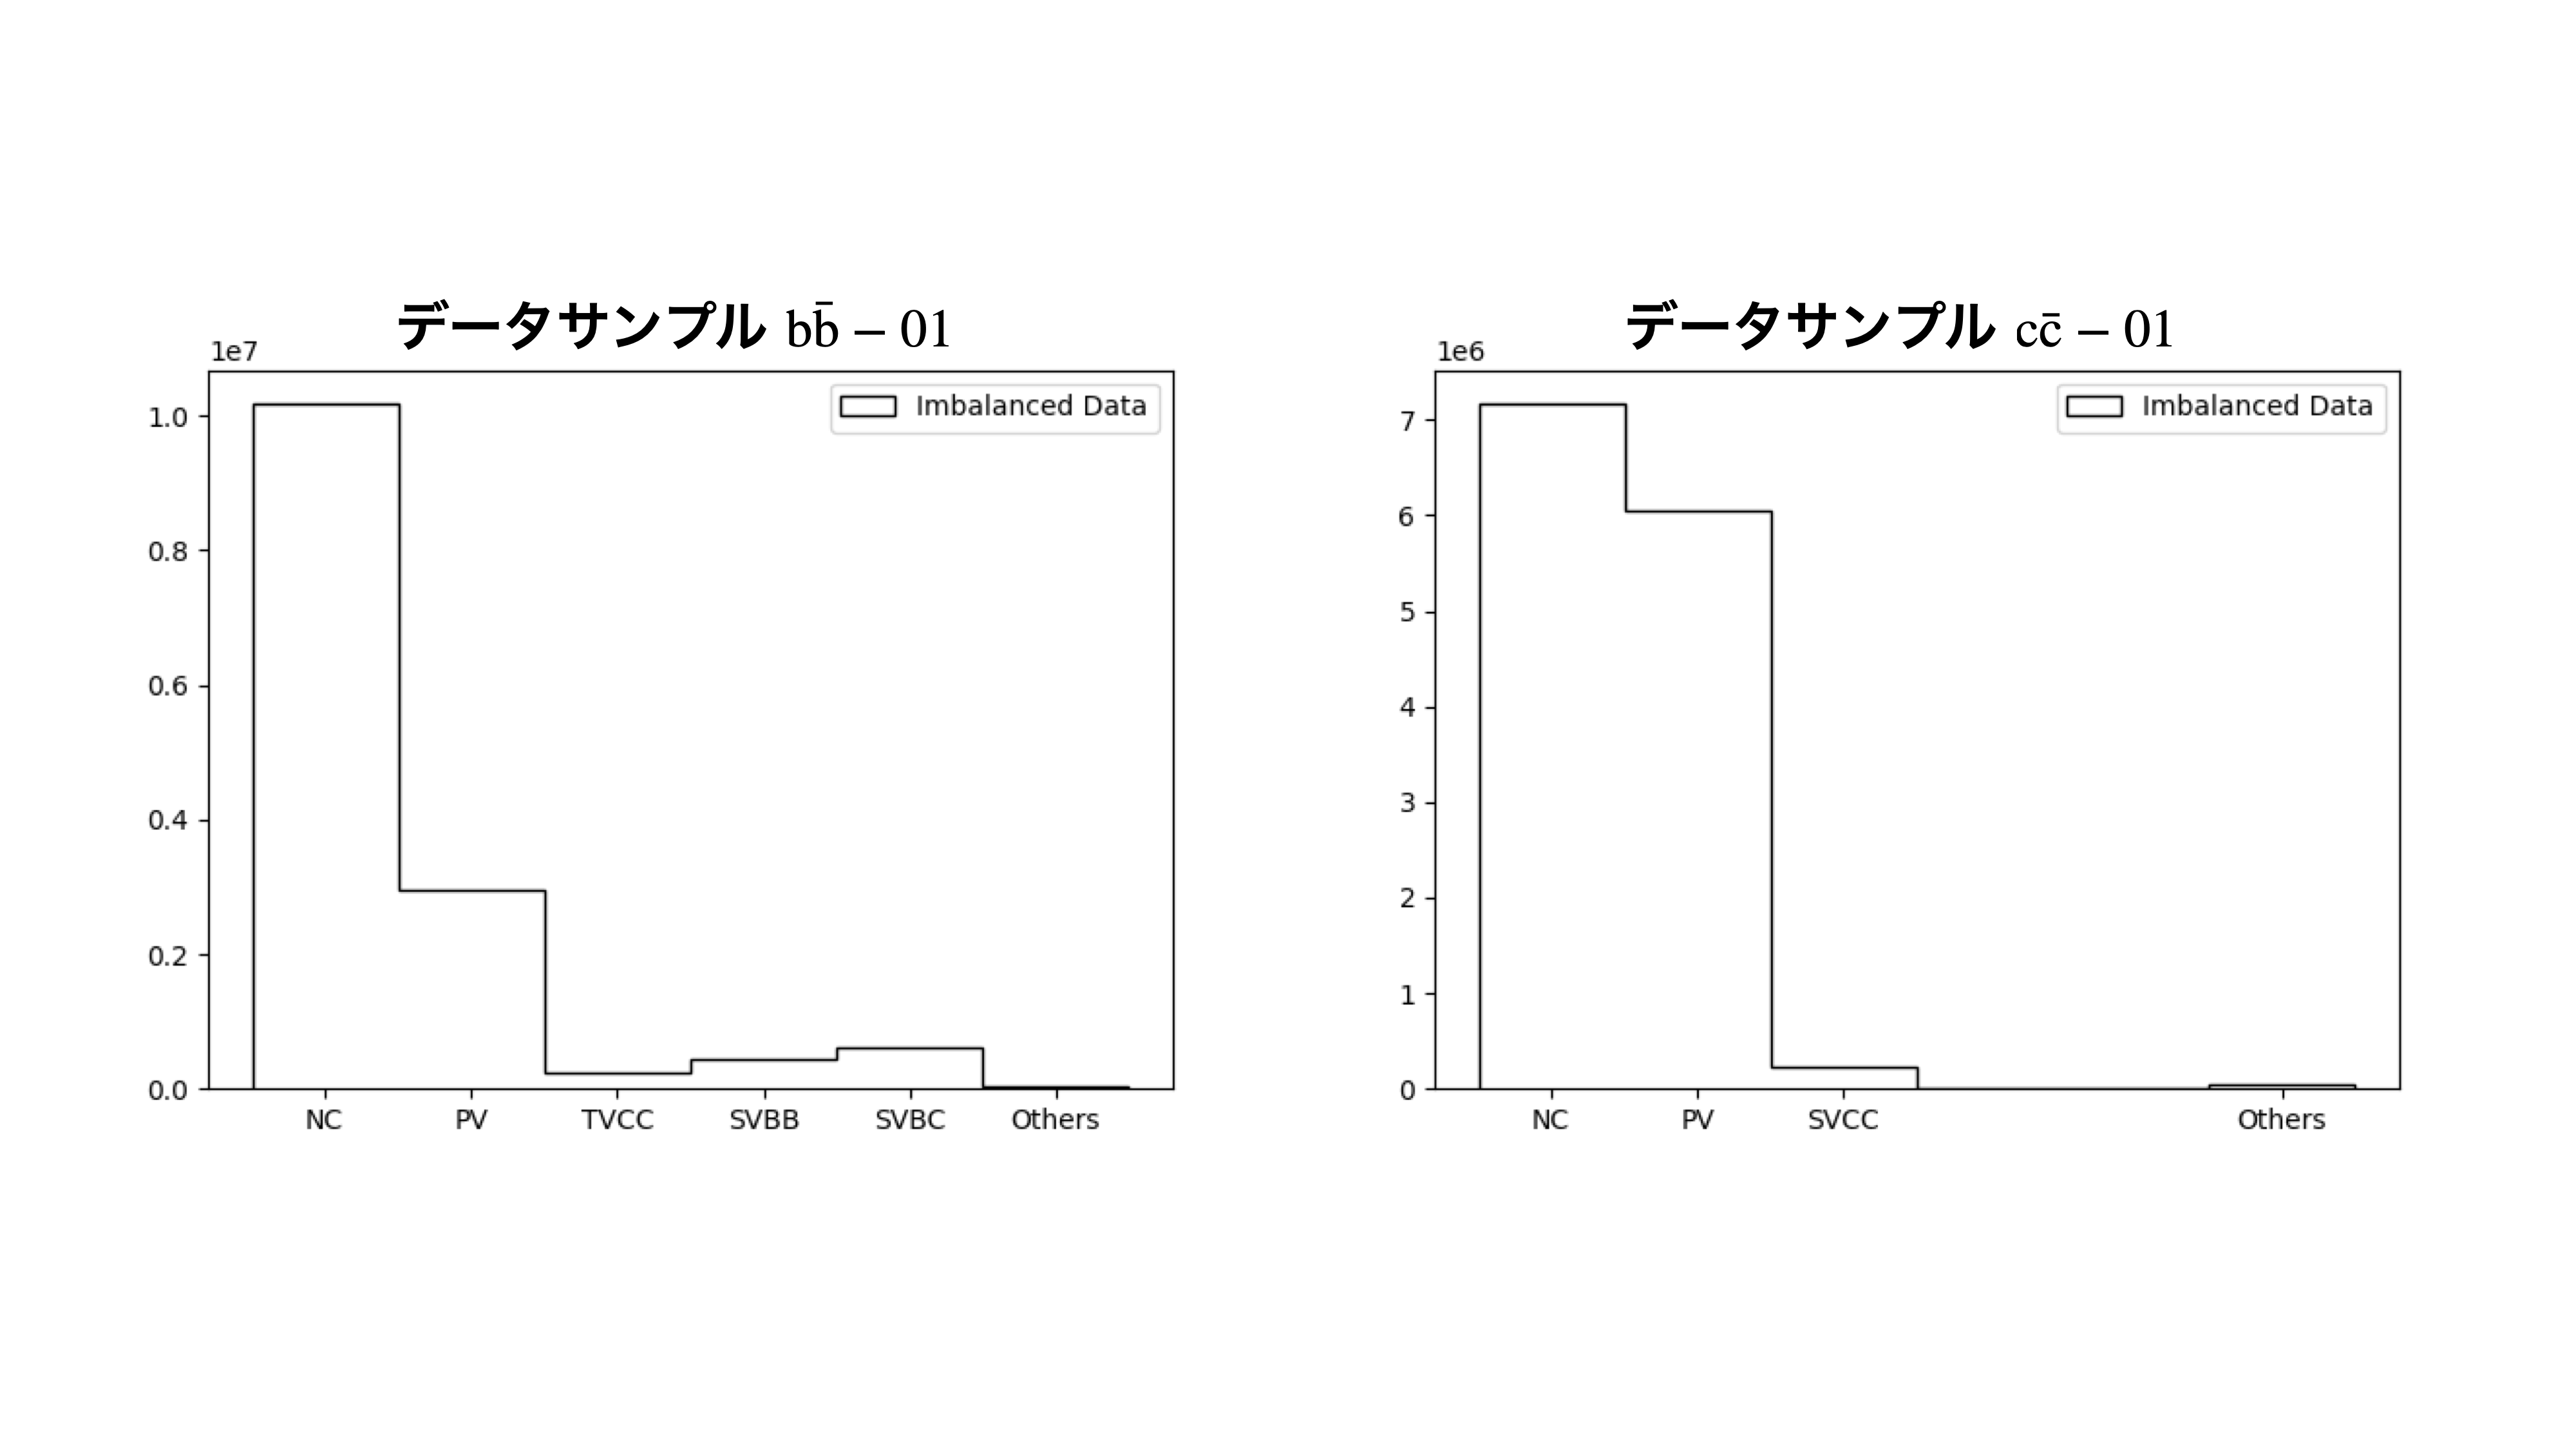
\includegraphics[trim = 100 200 100 150, width=0.9\textwidth, clip]{Figure/3Networks/3-3-2-1ImbalancedData.png}
 \caption[各終状態での分類クラスのデータ数の比]{各終状態での分類クラスのデータ数の比。図左が終状態$\rm b\bar{b}$、図右が終状態$\rm c\bar{c}$である。終状態$\rm c\bar{c}$ではSVCC以外のSVが基本的に存在しない為、終状態$\rm b\bar{b}$と比較してPVの比率が多くなっている。}
 \label{3-3-2-1ImbalancedData}
\end{figure}

このような不均衡データについては、少数クラスのデータをかさ増しするオーバーサンプリング、多数クラスのデータを間引くアンダーサンプリング、損失関数のコストに重みをつけるコスト考慮型学習の主に三つの対応策が存在する。
オーバーサンプリングやアンダーサンプリングは過学習や情報の欠損などの問題を抱えているため、本研究では基本的にコスト考慮型学習を用いる。
ただし、二つの終状態のデータを単純に足し合わせた場合、共通する分類クラスであるNCやPVがより顕著になり、他クラスの学習が不十分になると考えられる。
このためNCやPVに関しては各終状態毎に半分にランダムサンプリングした後、終状態$\rm b\bar{b}$と$\rm c\bar{c}$を足し合わせた。
最終的な訓練データでの分類クラスのデータ数の比を図\ref{3-3-2-2ImbalancedData}に示す。

\begin{figure}[htbp]
 \centering
 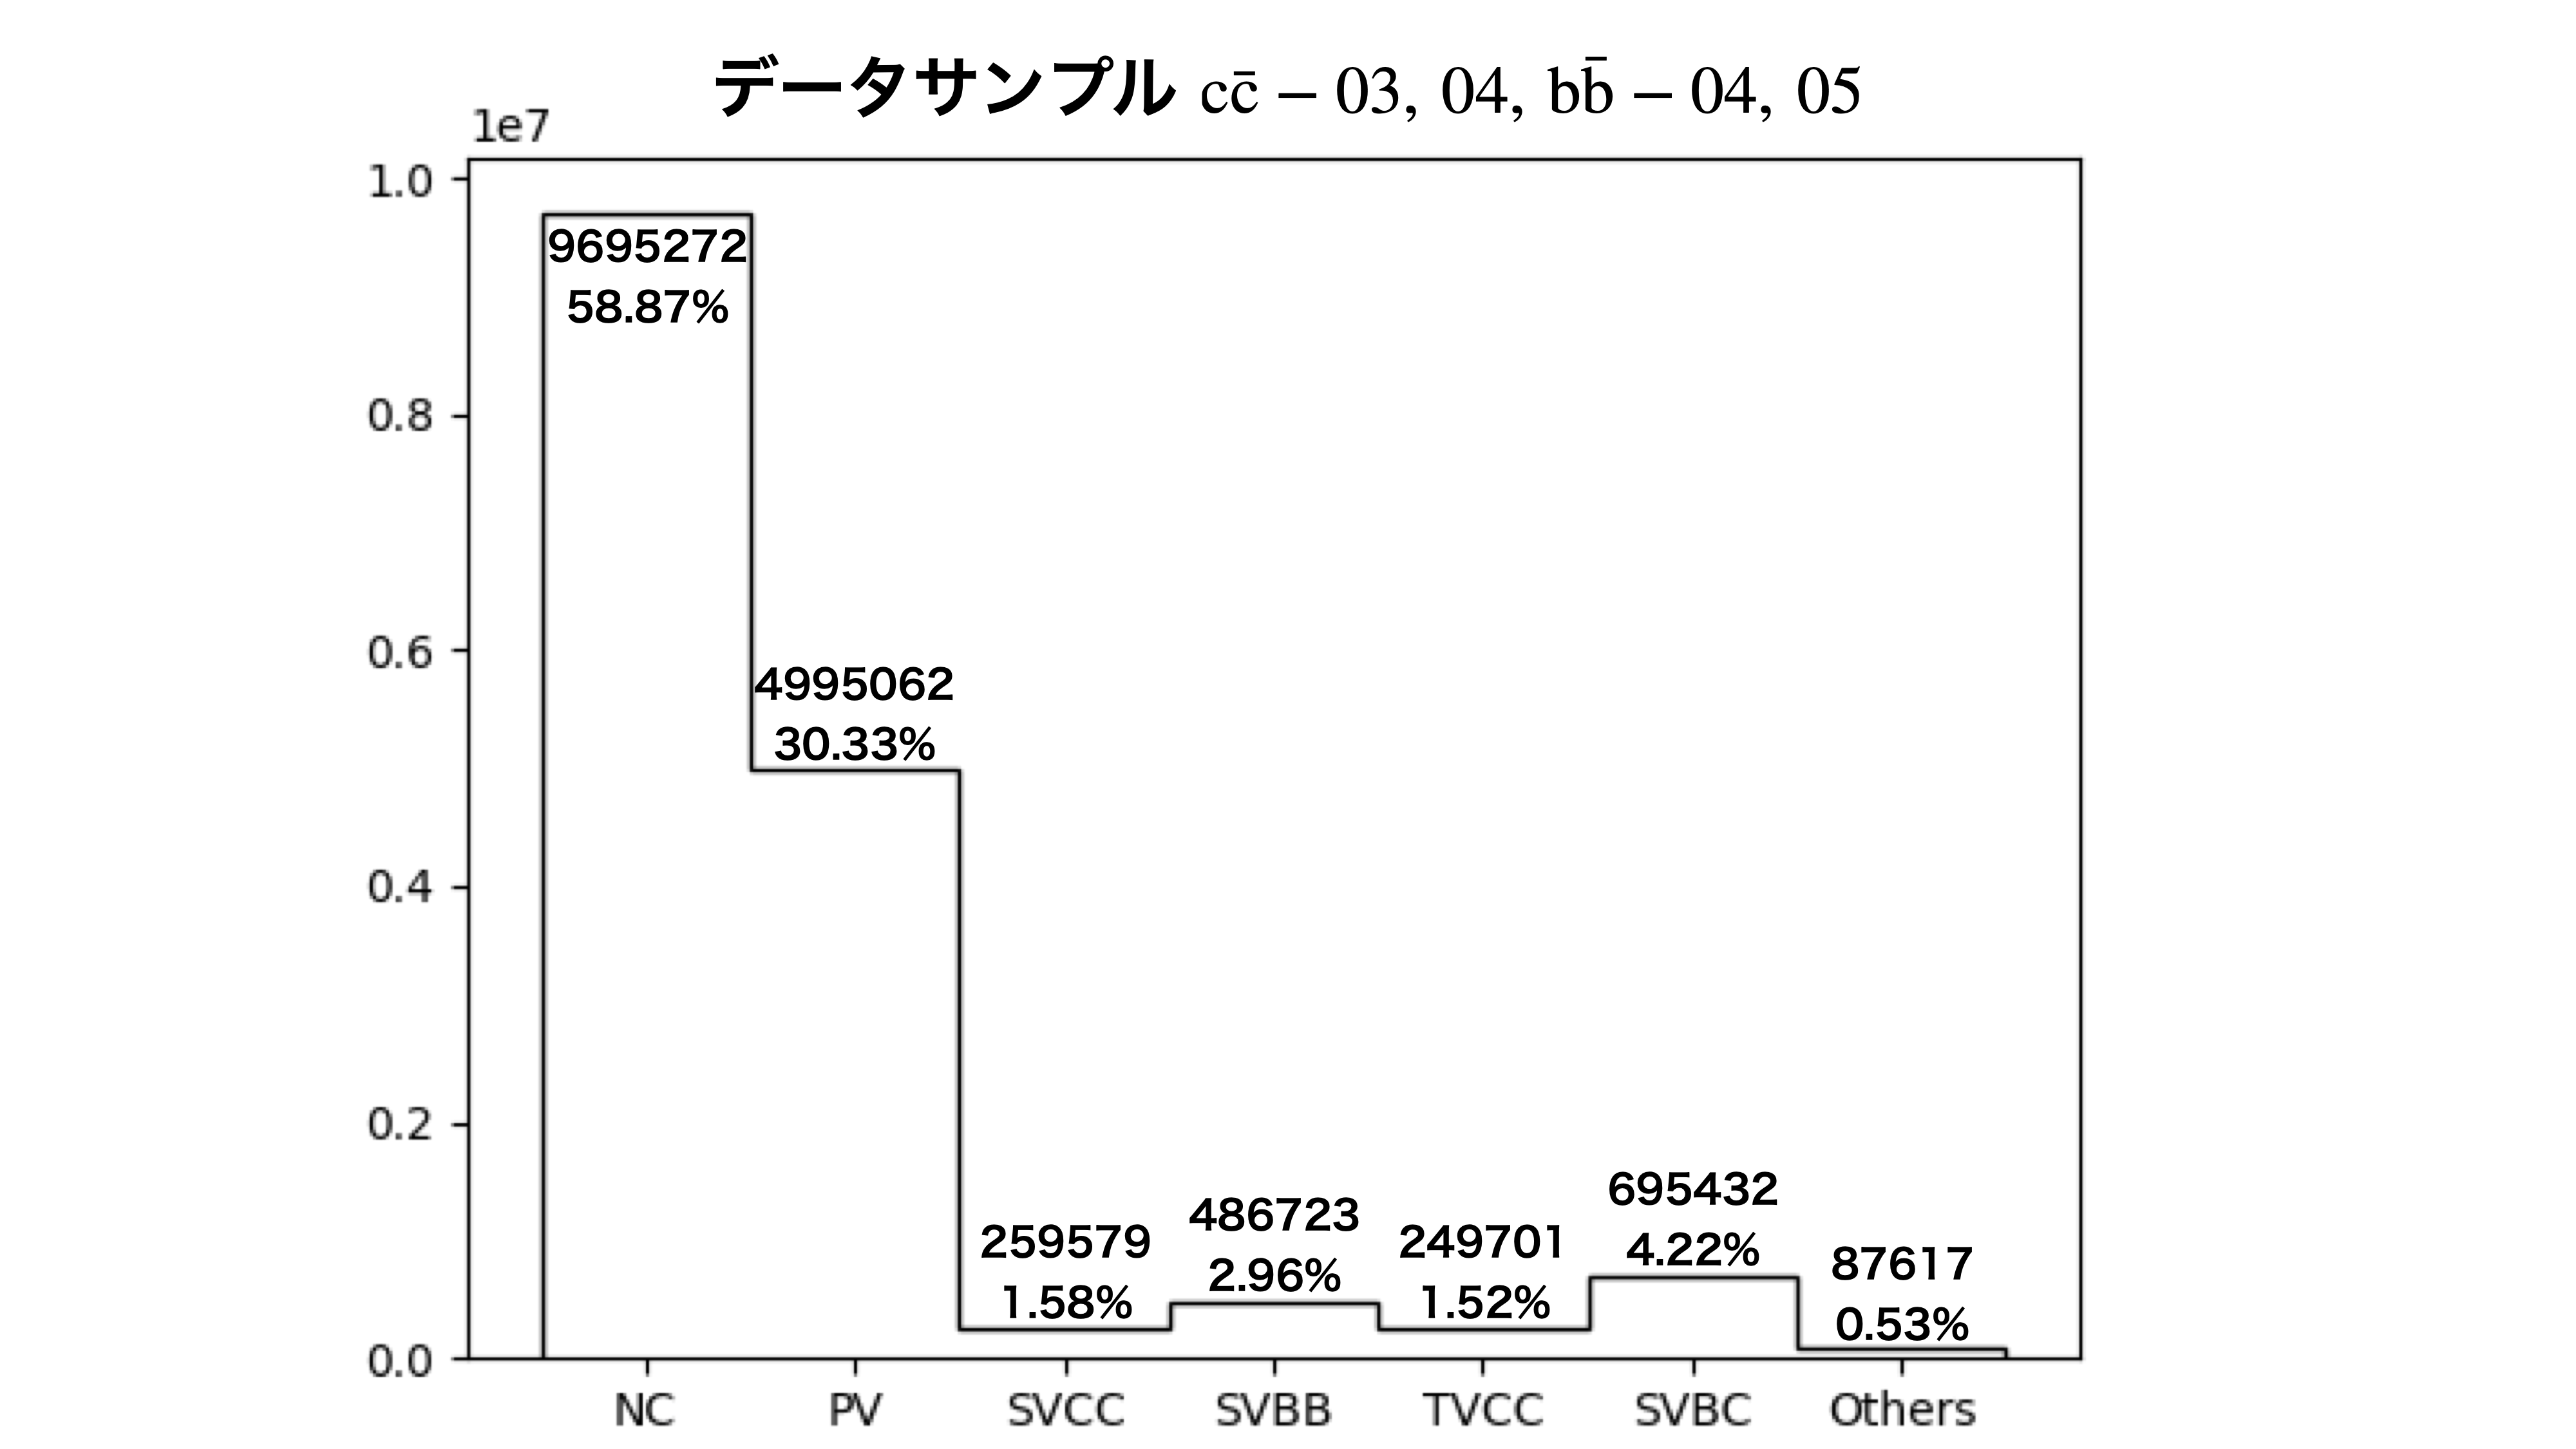
\includegraphics[width=1.0\textwidth]{Figure/3Networks/3-3-2-2ImbalancedData.png}
 \caption[訓練データでの分類クラスのデータ数の比]{訓練データでの分類クラスのデータ数の比。実際に使用する訓練データではNCとPVのカテゴリで全体の$9$割程度となっており、非常に不均衡なデータとなっている。}
 \label{3-3-2-2ImbalancedData}
\end{figure}

損失関数$L$は分類問題である崩壊点の種類に関しての損失関数$L_{\rm CE}$と回帰問題である崩壊点の位置に関しての損失関数$L_{\rm LMSE}$の二つの合計となる。

本研究では、コスト考慮型学習として損失関数$L_{\rm CE}$の各クラスへの重みは、分類クラスのデータ数の比の逆数を使用し不均衡データへ対策を行なった。
ここでは最も数の少ないOthersの重みを$1$としている。
\begin{equation}
 \begin{split}
 L_{\rm CE} = & - 0.0090\  t_{\rm NC} \log{(y_{\rm NC})} - 0.0175\  t_{\rm PV} \log{(y_{\rm PV})} \\
       & - 0.3375\  t_{\rm SVCC} \log{(y_{\rm SVCC})} - 0.1800\  t_{\rm SVBB} \log{(y_{\rm SVBB})}\\
       & - 0.3509\  t_{\rm TVCC} \log{(y_{\rm TVCC})} - 0.1260\  t_{\rm SVBC} \log{(y_{\rm SVBC})}\\
       & - 1.0\  t_{\rm Others} \log{(y_{\rm Others})}\\
 \end{split}
\end{equation}
ここで、$t_{\rm NC},\ t_{\rm PV},\ t_{\rm SVCC},\ t_{\rm SVBB},\ t_{\rm TVCC},\ t_{\rm SVBC},\ t_{\rm Others}$はそれぞれの分類クラスについての正解ラベルである。
また、$y_{\rm NC},\ y_{\rm PV},\ y_{\rm SVCC},\ y_{\rm SVBB},\ y_{\rm TVCC},\ y_{\rm SVBC},\ y_{\rm Others}$はそれぞれの分類クラスについてネットワークで予想された確率である。

崩壊点の位置についての損失関数$L_{\rm LMSE}$として平均二乗誤差を使用した。
ただし、図\ref{3-1-2-3VertexPositions}からも分かるように、崩壊点の位置は非常に広い範囲に分布しているため、出力や正解ラベルの自然対数を使用し
\begin{equation}
 \begin{split}
 L_{\rm LMSE} = (\ln{(t_{\rm Position}+1)} - \ln{(y_{\rm Position}+1)})^2
 \end{split}
\end{equation}
とした。
ここで、$t_{\rm Position},\ y_{\rm Position}$はそれぞれLCFIPlusのフィッターで予想された崩壊点の位置、ネットワークで予想された崩壊点の位置である。

以上より、飛跡対についてのネットワークの損失関数$L$は
\begin{equation}
 \begin{split}
 L & = w_{\rm vertex} L_{\rm CE} + w_{\rm position} L_{\rm LMSE}
 \end{split}
\end{equation}
となる。
ここで、$w_{\rm vertex},\ w_{\rm position}$は各損失関数$L_{\rm CE},\ L_{\rm LMSE}$への重みである。

本ネットワークでは崩壊点の位置を学習した後に崩壊点の種類の分類を行なった。
これは崩壊点の位置、あるいはそのような情報を抽出できるネットワークのパラメータを利用して、崩壊点の種類の分類を行なって欲しいという狙いからである。
これは転移学習 (Transfer Learning, TL) やファインチューニングという手法\footnote{これらの手法ではあらかじめ学習済みのネットワークを別の問題解決に活用するテクニックである}に似た発想であるが、今回はこれら二つの手法とは異なり、ネットワークの重みは全て再学習に使用している。
学習は以下の手順で行う。

\begin{enumerate}
 \item $(w_{\rm vertex},\ w_{\rm position})=(0.1,\ 0.9)$、$1000\ \mathrm{epoch}$、学習率${\rm LR}=0.001$
 \item $(w_{\rm vertex},\ w_{\rm position})=(0.9,\ 0.1)$、$1500\ \mathrm{epoch}$、学習率${\rm LR}=0.001$
 \item $(w_{\rm vertex},\ w_{\rm position})=(0.95,\ 0.05)$、$500\ \mathrm{epoch}$、学習率${\rm LR}=0.0001$
\end{enumerate}

また、重み更新の最適化手法としてSGDを用いた。
これは、Adamなどでは収束が早すぎ、過学習になる恐れがあったためである。
学習には$13175508$サンプル、検証には$3293878$サンプルのデータを使用した。
ネットワークの学習可能な重みのパラメータ数を表\ref{ParametersforPairModel}に示す。

\begin{table}[htb]
 \centering
 \small
 \scalebox{0.8}{
  \begin{tabular}{l c c c}\hline
    層の名称 & 出力の形状 & パラメータ数 & 接続先\\\hline\hline
    Pair Input & (None, 44) & 0 & \\\hline\hline
    Dense 1 & (None, 256) & 11520 & Pair Input[0][0]\\\hline
    Batch Normalization 1 & (None, 256) & 1024 & Dense 1[0][0]\\\hline
    Activation ReLU 1 & (None, 256) & 0 & Batch Normalization 1[0][0]\\\hline
    Dense 2 & (None, 256) & 65792 & Activation ReLU 1[0][0]\\\hline
    Batch Normalization 2 & (None, 256) & 1024 & Dense 2[0][0]\\\hline
    Activation ReLU 2 & (None, 256) & 0 & Batch Normalization 2[0][0]\\\hline
    Dense 3 & (None, 256) & 65792 & Activation ReLU 2[0][0]\\\hline
    Batch Normalization 3 & (None, 256) & 1024 & Dense 3[0][0]\\\hline
    Activation ReLU 3 & (None, 256) & 0 & Batch Normalization 3[0][0]\\\hline\hline
    Vertex Dense &  (None, 7) & 1799 & Activation ReLU 3[0][0]\\\hline
    Vertex Output & (None, 7) & 0 & Vertex Dense[0][0]\\\hline\hline
    Position Output & (None, 1) & 257 & Activation ReLU 3[0][0]\\\hline\hline
  \end{tabular}
  }
  \caption{飛跡対についてのネットワークにおける訓練可能なパラメータ}
  \label{ParametersforPairModel}
\end{table}


%%%%%%%%%%%%%%%%%%%%%%%%%%%%%%%%%%%%%%%%%%%%%%%%%%%%%%%%%%%%%%%%%%%%%%%%
\subsection{ネットワークの評価} \label{Net:PM:PerformanceofPM}

ネットワークの評価は1. ネットワーク間の比較、2. ネットワーク内の理解の二つの観点によって行う。
本ネットワークでは、1. ネットワーク間の比較については入力変数やネットワーク構造の異なる幾つかのネットワークのモデルについて比較を行う。
2. ネットワーク内の理解についてはt分布型確率的近傍埋め込み法(t-Distributed Stochastic Neighbor Embedding, t-SNE\cite{t-SNEpaper})を用いた次元削減によって、ネットワークによる情報の抽出や各クラスの分離について議論する。\\

1. ネットワーク間の比較\\

深層学習を取り扱う上で気を付けなければならない問題として、ネットワークの怠け(Lazy)が存在する。
ネットワークの怠けとは、ある入力変数について、特定の要素にのみ注目する、あるいは特定の要素を無視してしまうという問題である。
飛跡対についてのネットワークでは、深層学習が取り扱いづらい共分散を入力している。
ここではネットワークが共分散をどの程度取り扱えているかを評価するため、共分散を含んだ入力変数を用いたモデルAと含んでいないモデルBを構築し比較を行なった。
ここでネットワークの構造として、図\ref{3-3-1-1PairModel}を使用し、そのようなネットワークの構造をネットワーク$1$と呼ぶことにする。

また、\ref{Net:Data:TrackInformationandPreprocessing}節でも述べたように本研究における崩壊点の種類の分離において、崩壊点の位置の再構成は必須である。
したがって、そのような崩壊点の位置についての情報を再構成し、適切に処理出来ているかを把握するため、本来回帰問題の正解ラベルとして用いているLCFIPlusによって予想された崩壊点の位置についての情報を出力層の直前で入力するネットワーク2を構築した。
更に、ネットワーク自体が予想した崩壊点の位置を明示的に入力に使用したネットワーク3の構築を行った。
これらネットワーク2、ネットワーク3を使用したモデルをそれぞれモデルC、モデルDとし前述のモデルA、モデルBとの比較を行なった。
それぞれのモデルの詳細を表\ref{EvalationModels}にまとめる。

\begin{figure}[htbp]
 \centering
  %\begin{tabular}{cccc}
  \begin{minipage}{1.0\textwidth}
  \centering
   \begin{minipage}{0.48\textwidth}
    \centering
    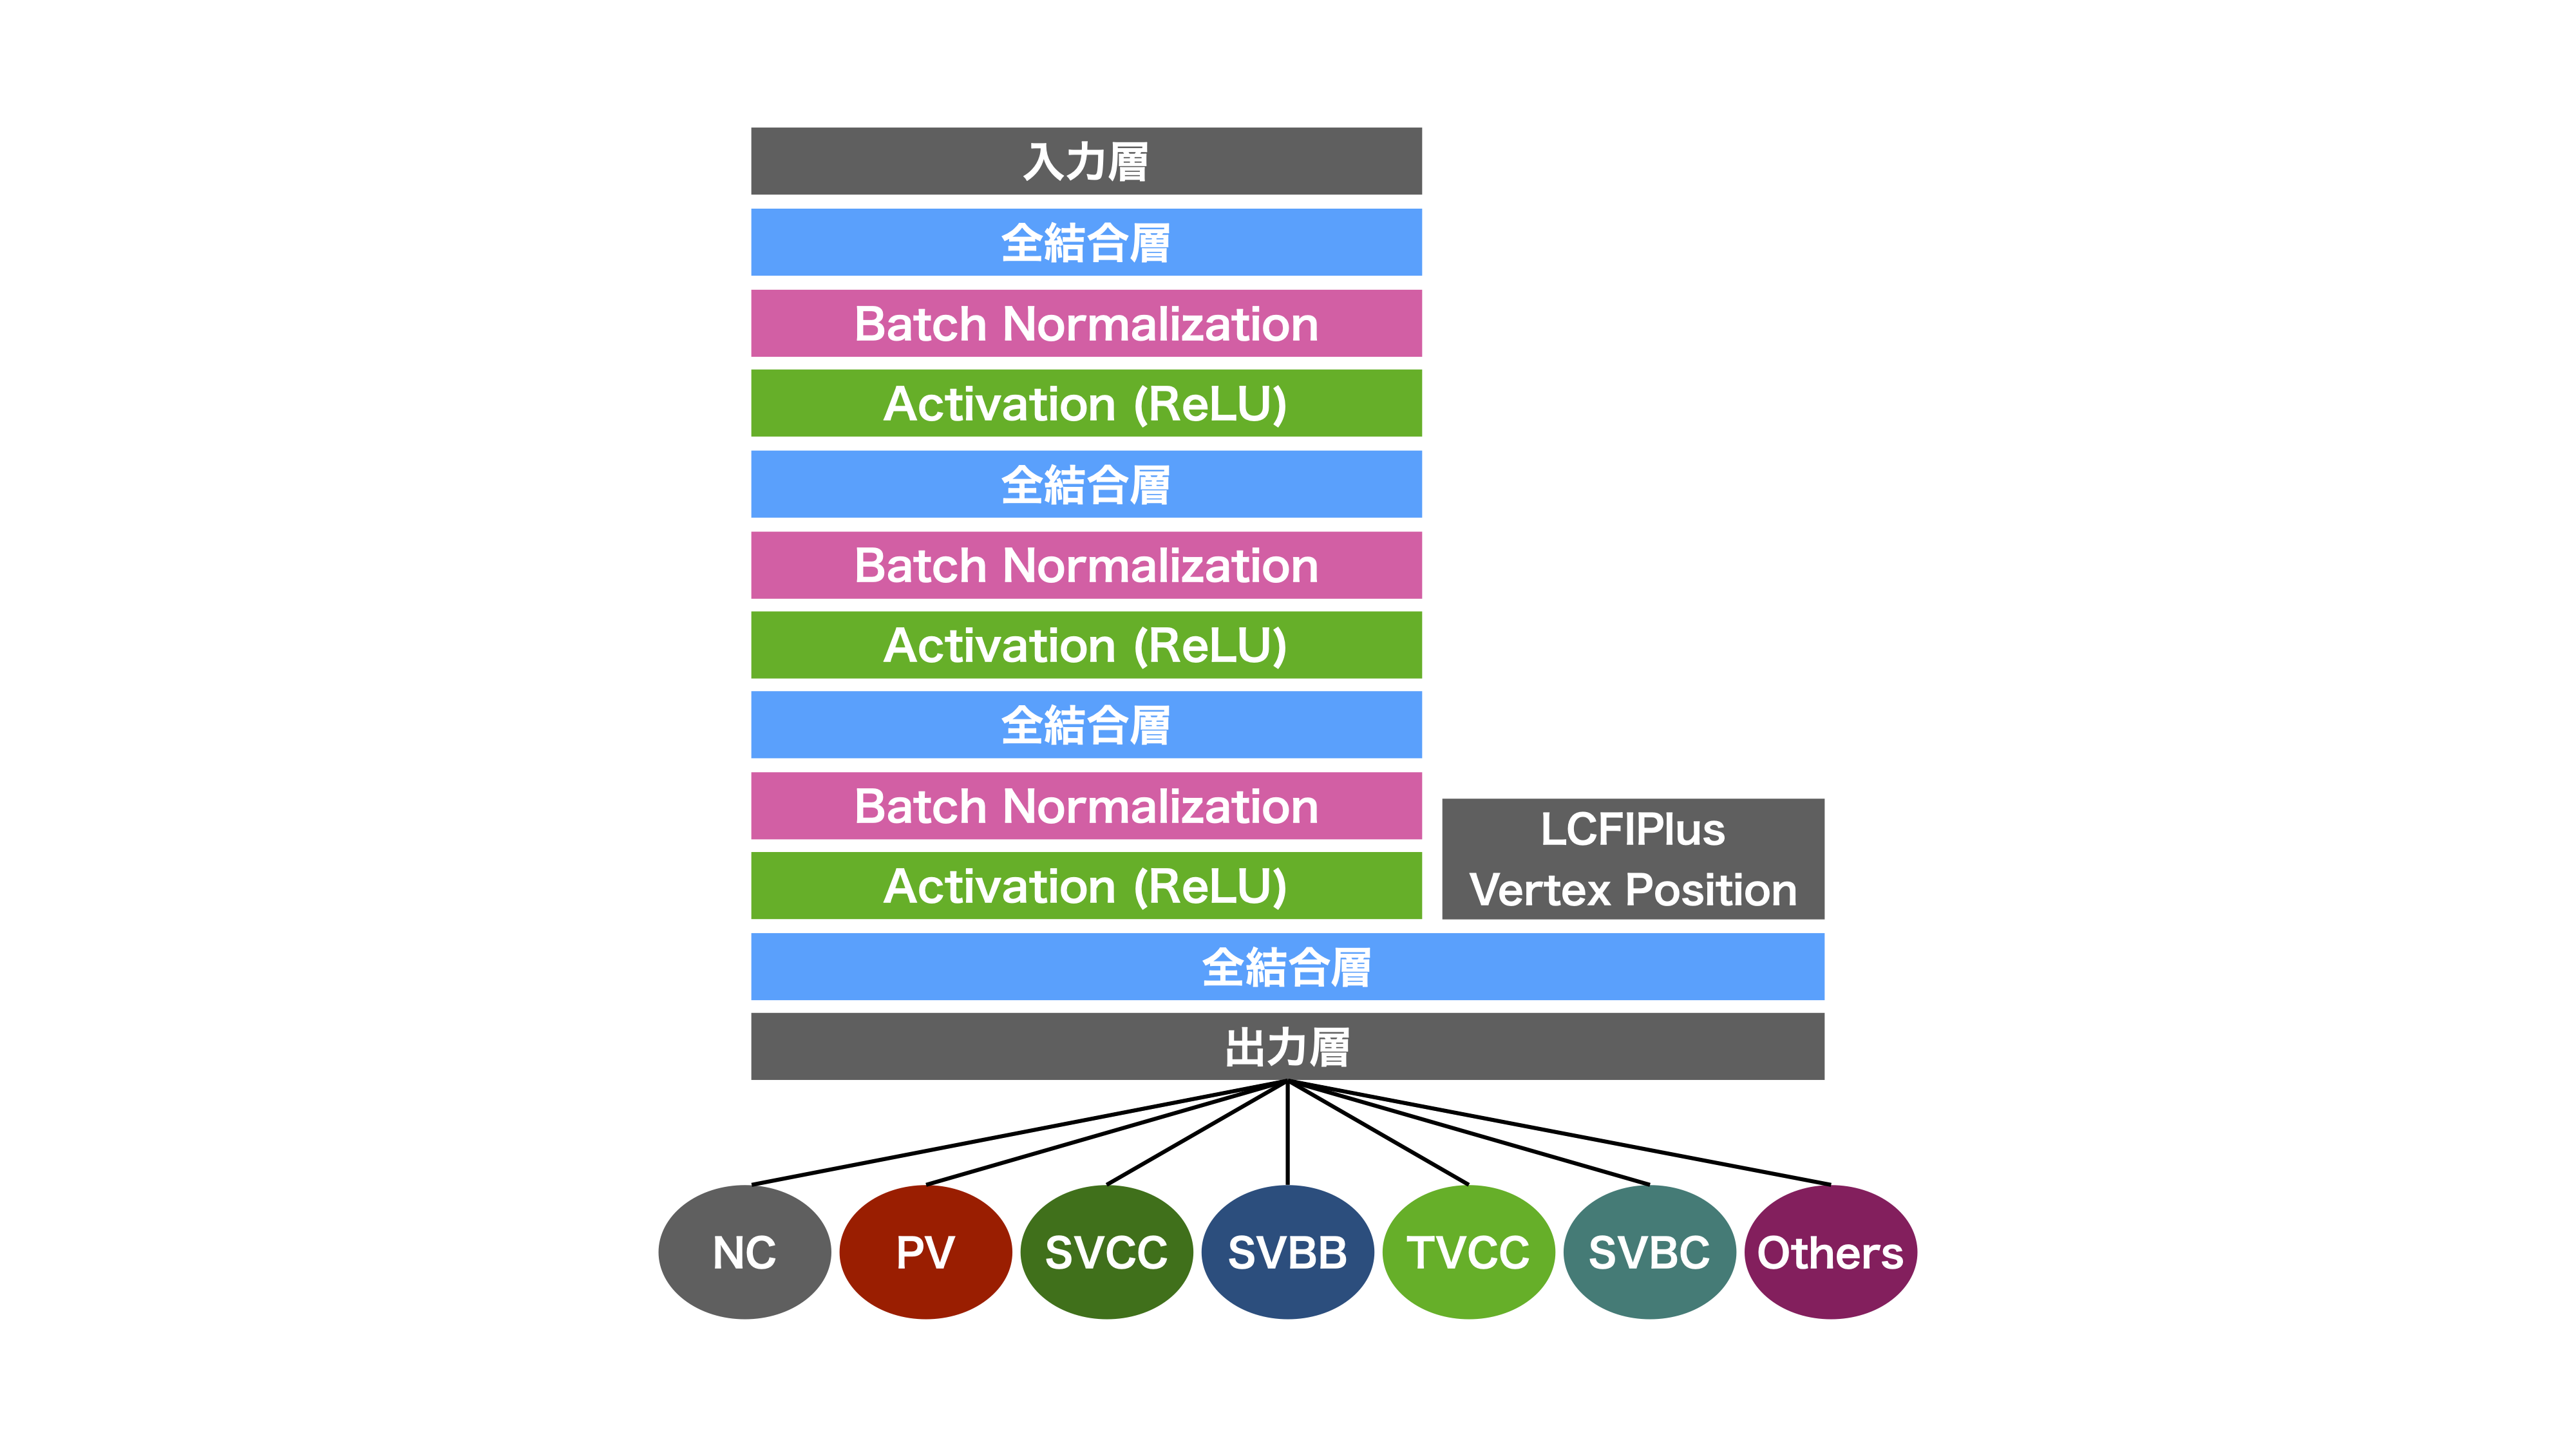
\includegraphics[trim = 200 0 200 0, width=1.0\textwidth, clip]{Figure/3Networks/3-3-3-1PairNetworkA.png}
    \subcaption{ネットワーク2}
    \label{3-3-3-1PairNetworkA}
   \end{minipage}
   \begin{minipage}{0.48\textwidth}
   \centering
    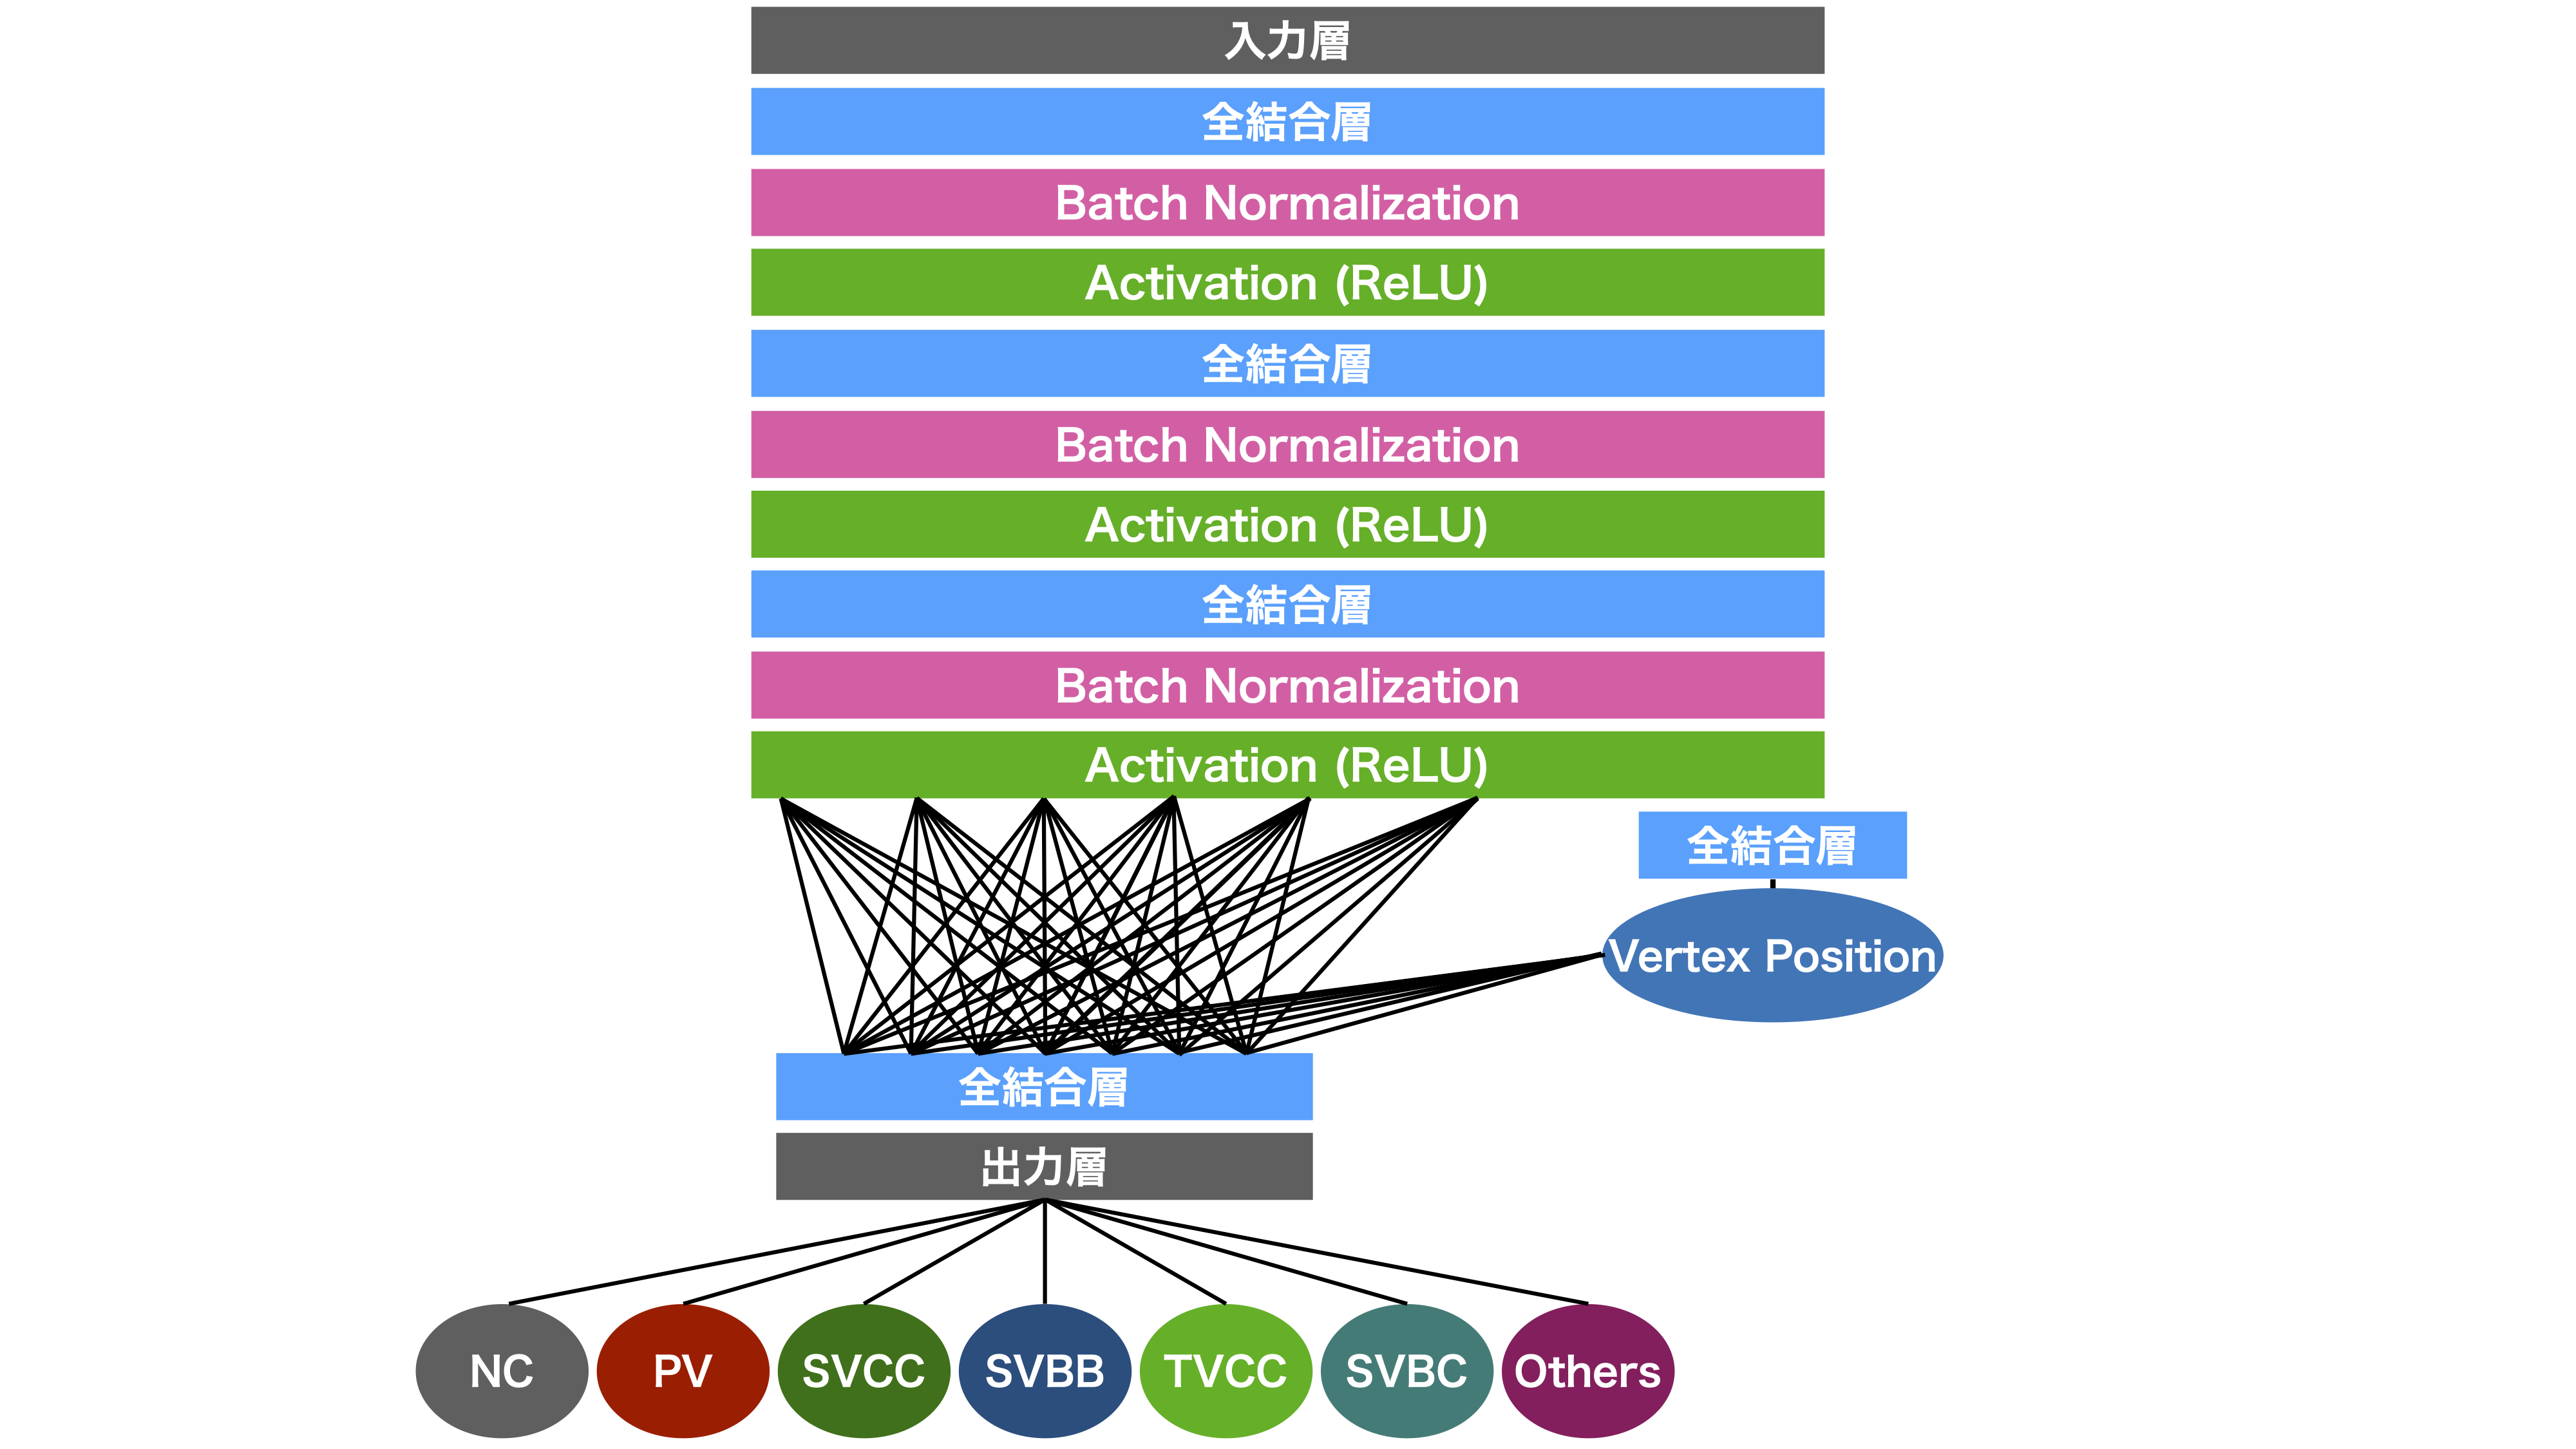
\includegraphics[trim = 200 0 200 0, width=1.0\textwidth, clip]{Figure/3Networks/3-3-3-1PairNetworkB.png}
    \subcaption{ネットワーク3}
    \label{3-3-3-1PairNetworkB}
   \end{minipage}
  \end{minipage}  
  \caption{評価のための飛跡対についてのネットワーク}
  \label{3-3-3-1PairNetworks}
 %\end{tabular}
\end{figure}

\begin{table}[htb]
 \centering
 \small
 \scalebox{0.85}{
  \begin{tabular}{c c c} \hline
    モデル & 入力変数 & ネットワーク\\\hline\hline
    モデルA & トラック・パラメータ、共分散行列、電荷、エネルギー & ネットワーク1\\
    モデルB & トラック・パラメータ、電荷、エネルギー & ネットワーク1\\
    モデルC & トラック・パラメータ、共分散行列、電荷、エネルギー、崩壊点の位置 & ネットワーク2\\
    モデルD & トラック・パラメータ、共分散行列、電荷、エネルギー & ネットワーク3\\\hline
  \end{tabular}
  }
  \caption{評価のための飛跡対についてのモデル}
  \label{EvalationModels}
\end{table}

比較は各クラス分類についての「ネットワークのスコアとその効率の変化」と「混合行列」の二つの指標を用いて行う。
また、本ネットワークは7クラス分類を行っているため、ある特定のクラスについてのスコアに閾値を設け、評価することは数学的に厳密に正しくない。
しかし、ここでは直感的な理解を優先し評価手法の一つとして採用している。

まず、ネットワークのスコアとクラス分類の効率の関係を図\ref{3-3-3-2Efficiency_Curve}に示す。
図の横軸はネットワークによって得られる各クラスのスコアに設けた閾値である。
また、縦軸は効率を示しており、実線で信号効率を、破線でバックグラウンド効率を表している。
ここでは、信号はそれぞれの特定のクラスとし、バックグラウンドはその特定のクラス以外の全てのクラスと定義している。
スコアに対して高い閾値を設けると信号・バックグラウンド共に効率は悪化し、逆に低い閾値であれば、全ての要素を信号であると判断してしまうため、両者の効率は最大となっている。
したがって、高い信号効率と低いバックグラウンド効率を実現できていれば、良い分類器であると判断できる。
図\ref{3-3-3-2Efficiency_Curve}ではNC・PV・Othersについては良く分類できているが、各SVについては殆ど見分けられていないことが分かる。

\begin{figure}[htbp]
 \centering
  %\begin{tabular}{cccc}
   \begin{minipage}{1.0\textwidth}
    \centering
    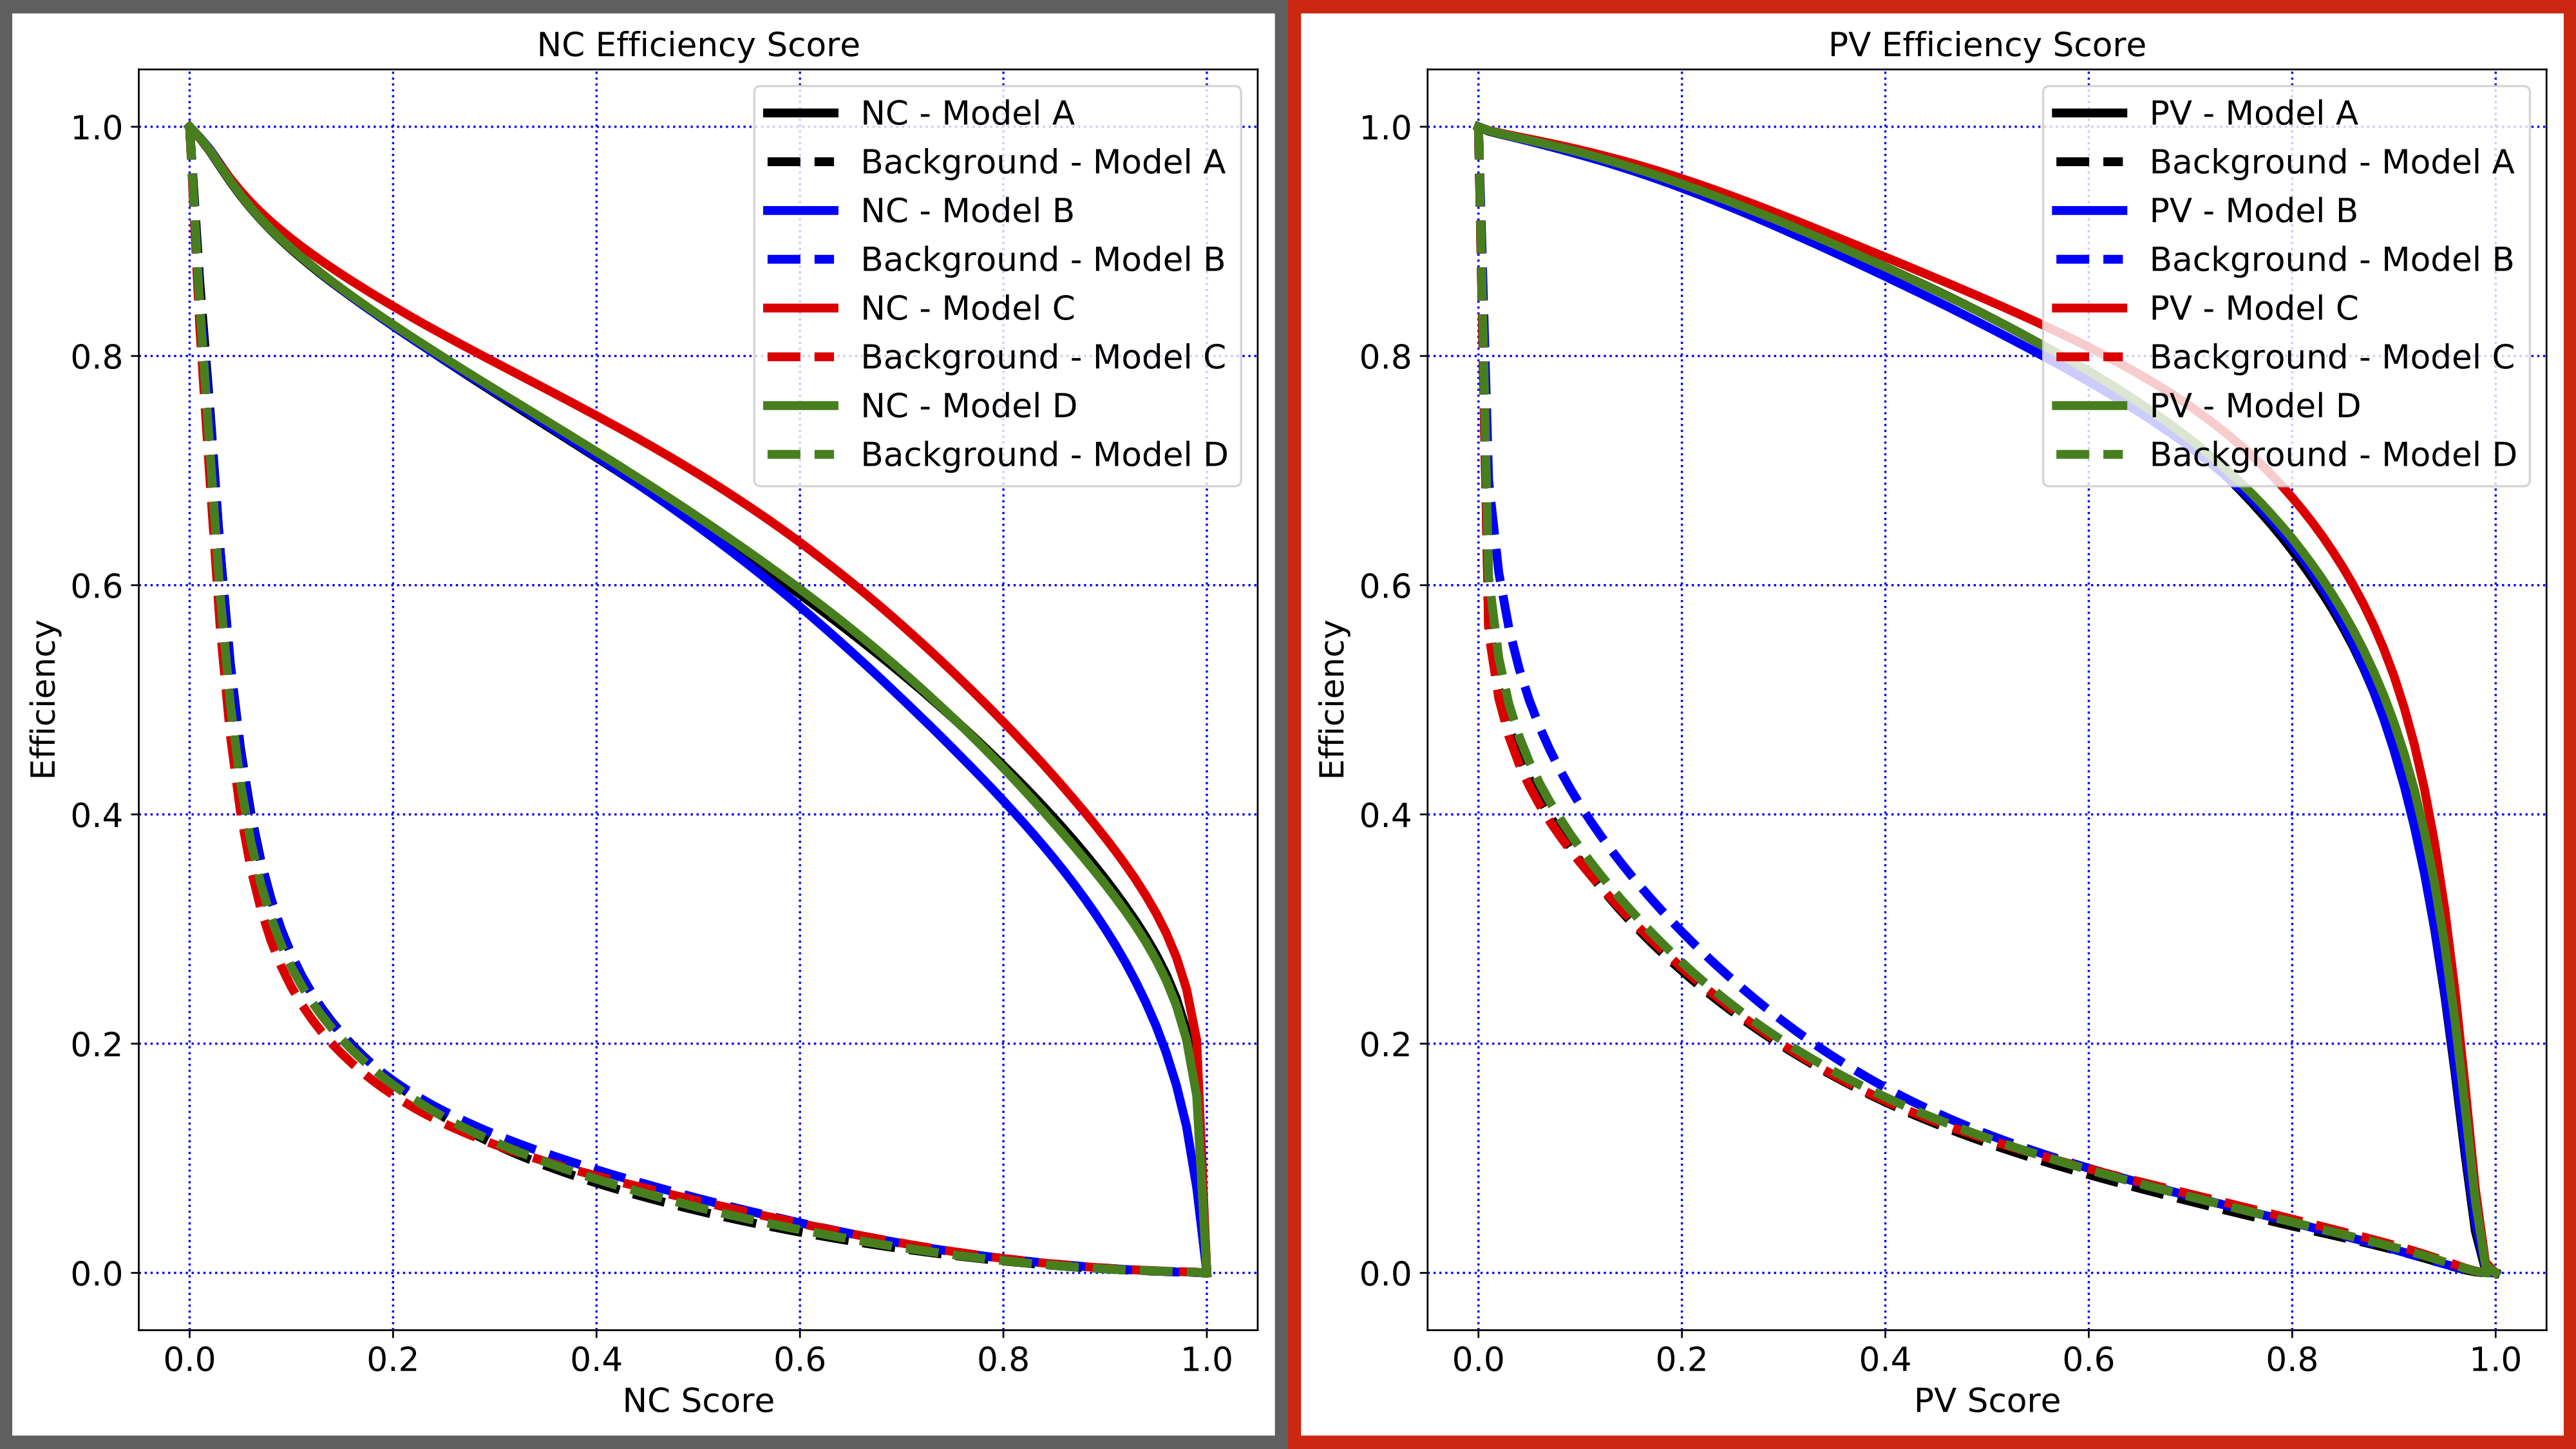
\includegraphics[width=1.0\textwidth, clip]{Figure/3Networks/3-3-3-2Efficiency_Curve_1.png}
   \end{minipage}

   \begin{minipage}{1.0\textwidth}
   \centering
    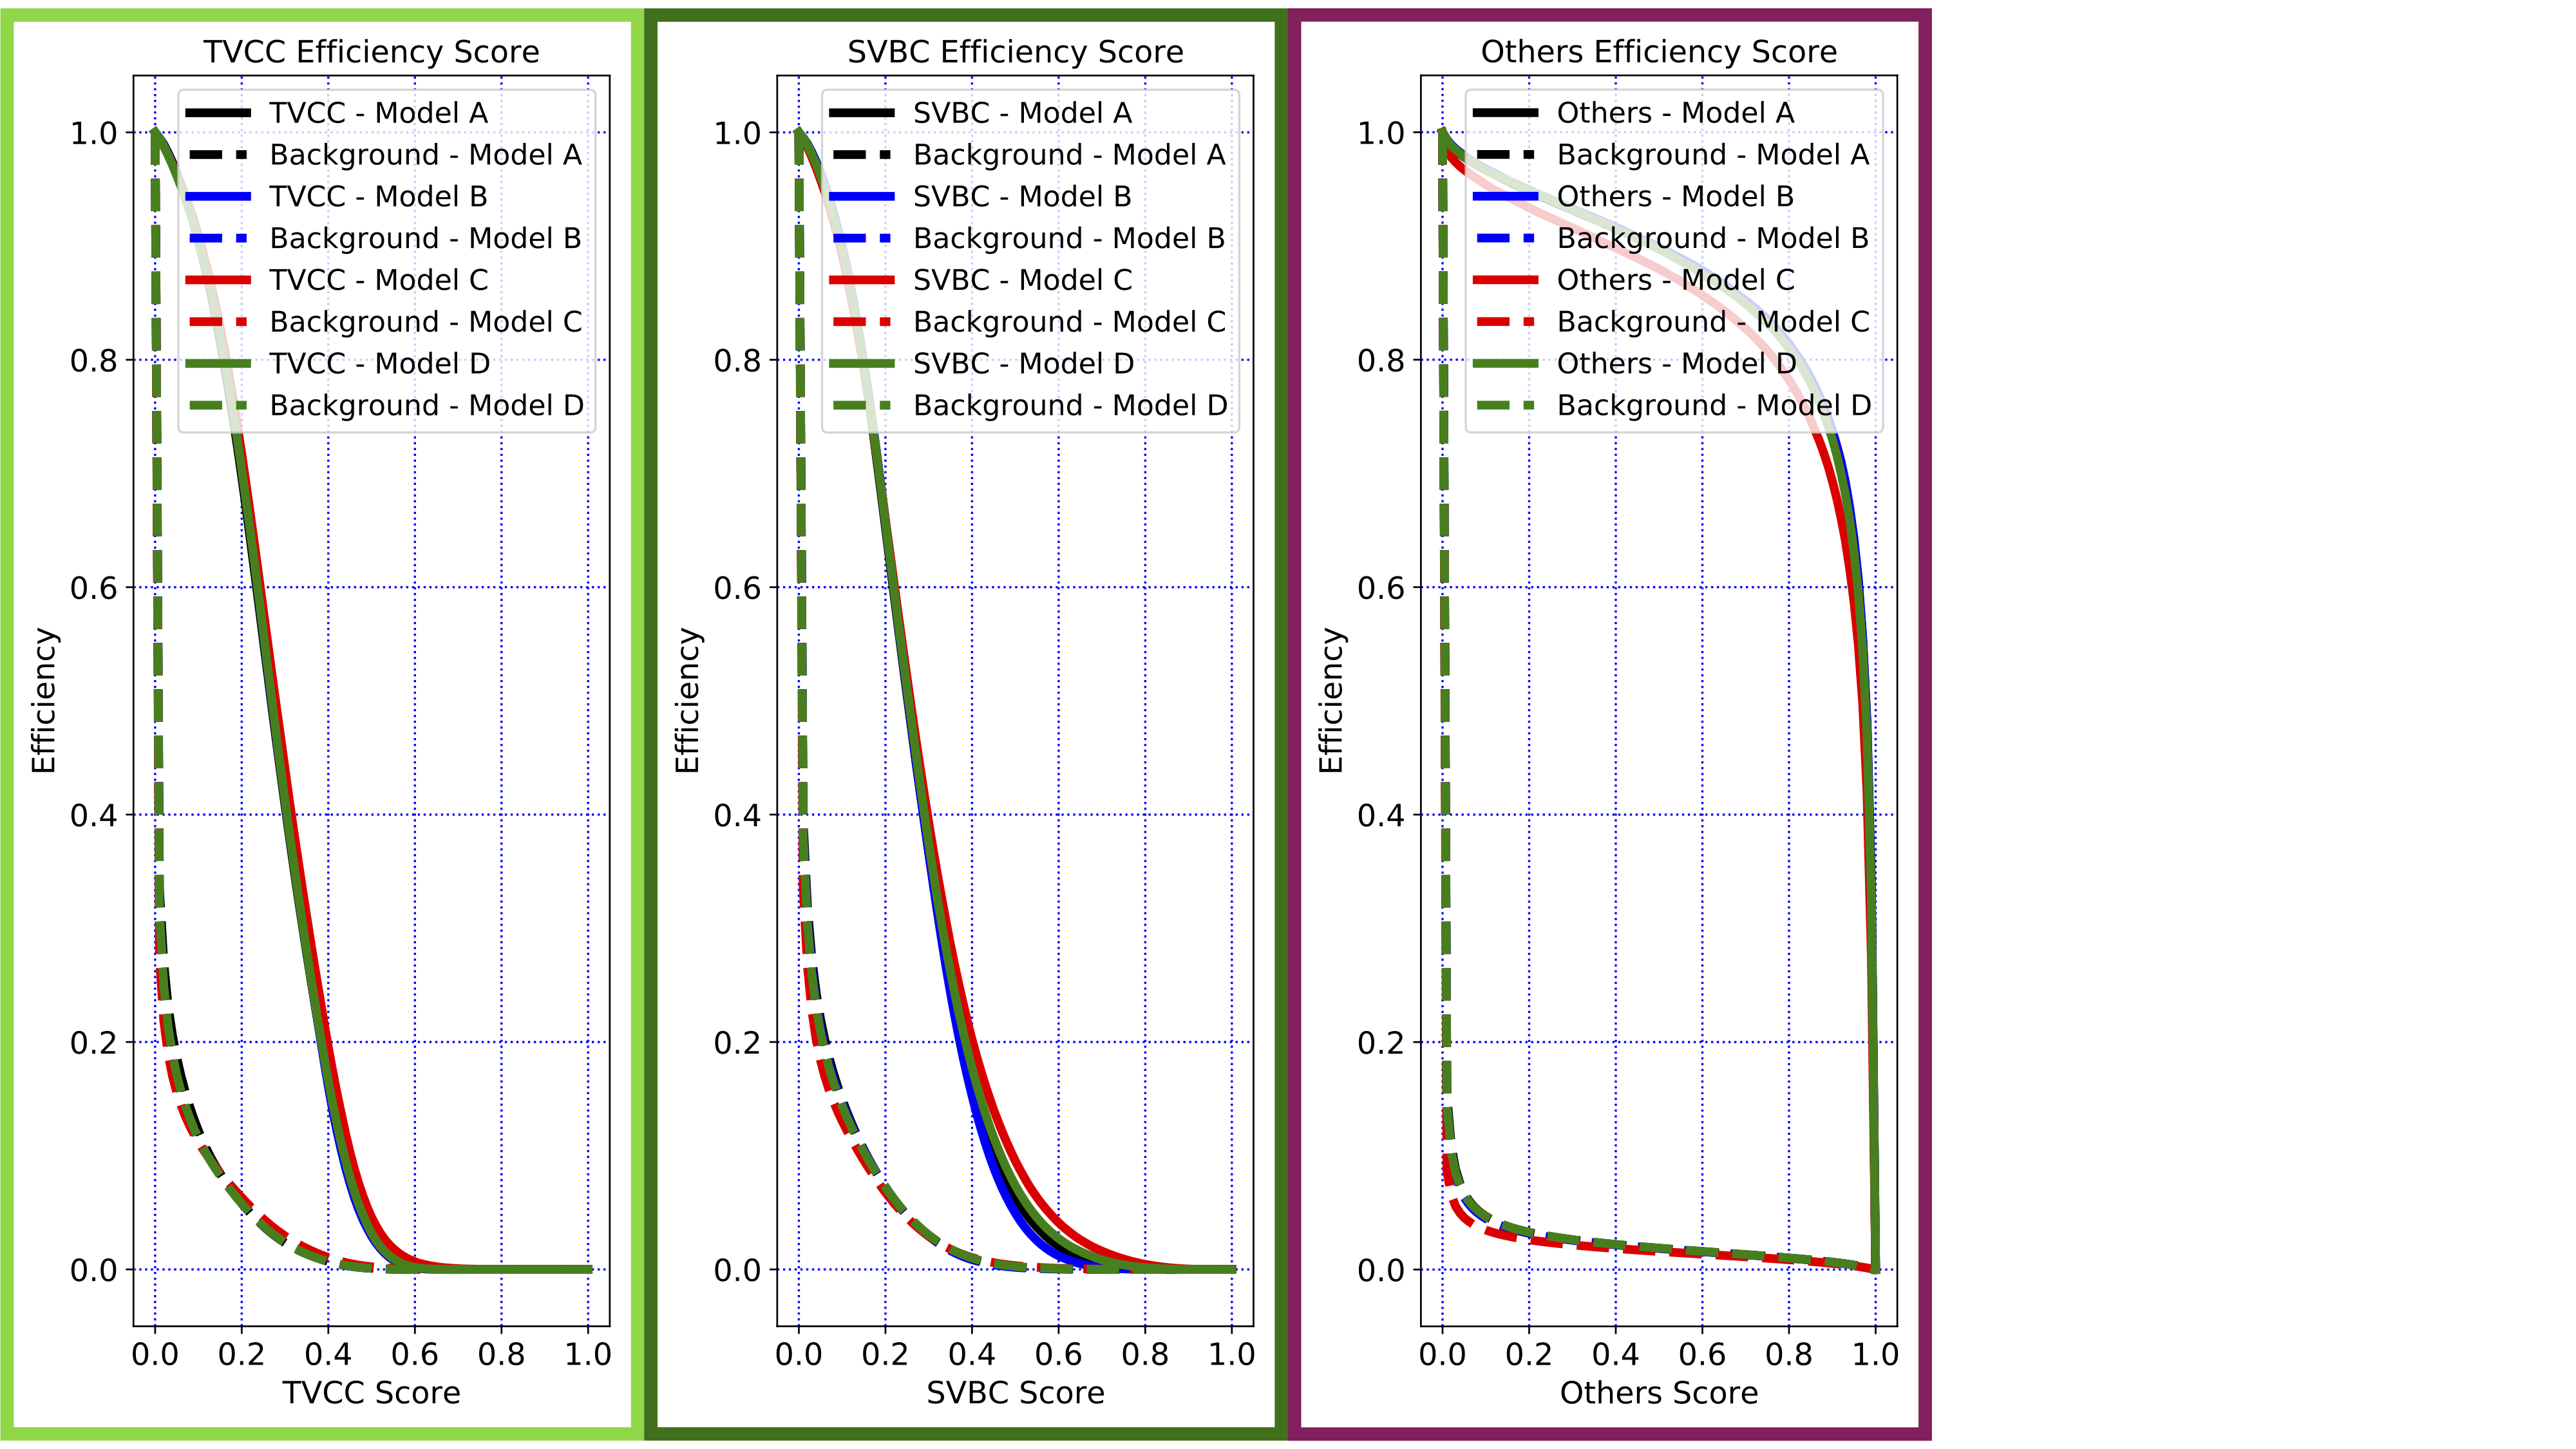
\includegraphics[width=1.0\textwidth, clip]{Figure/3Networks/3-3-3-2Efficiency_Curve_2.png}
   \end{minipage}
  \caption[ネットワークのスコアとクラス分類の効率の関係]{ネットワークのスコアとクラス分類の効率の関係。縦軸は効率、横軸はネットワークのスコアについての閾値である。実線は信号効率、破線はバックグラウンド効率である。黒線はモデルA、青線はモデルB、赤線はモデルC、緑線はモデルDをそれぞれ表している。}
  \label{3-3-3-2Efficiency_Curve}
 %\end{tabular}
\end{figure}

これら信号効率を縦軸にバックグラウンド効率を横軸に描画したものが図\ref{3-3-3-2ROC_Curve}である。
このような図を受信者操作特性(Receiver Operating Characteristic, ROC)曲線といい、ROC曲線はその曲線で囲んだ面積が大きければ性能が良いと判断できる。
したがって、より左側に張り出している分類器が最も良い性能となる。
ここでは、横軸を対数で表現しており、よりバックグラウンド効率の低い領域において、それぞれのモデルの比較を行っている。
図\ref{3-3-3-2ROC_Curve}ではどのクラスについてのモデル間の大きさ差異は見られない。
ただし、NCについてのみModel Bの性能が悪いという結果を得られた。

\begin{figure}[htbp]
 \centering
  %\begin{tabular}{cccc}
  \begin{minipage}{1.0\textwidth}
   \centering
    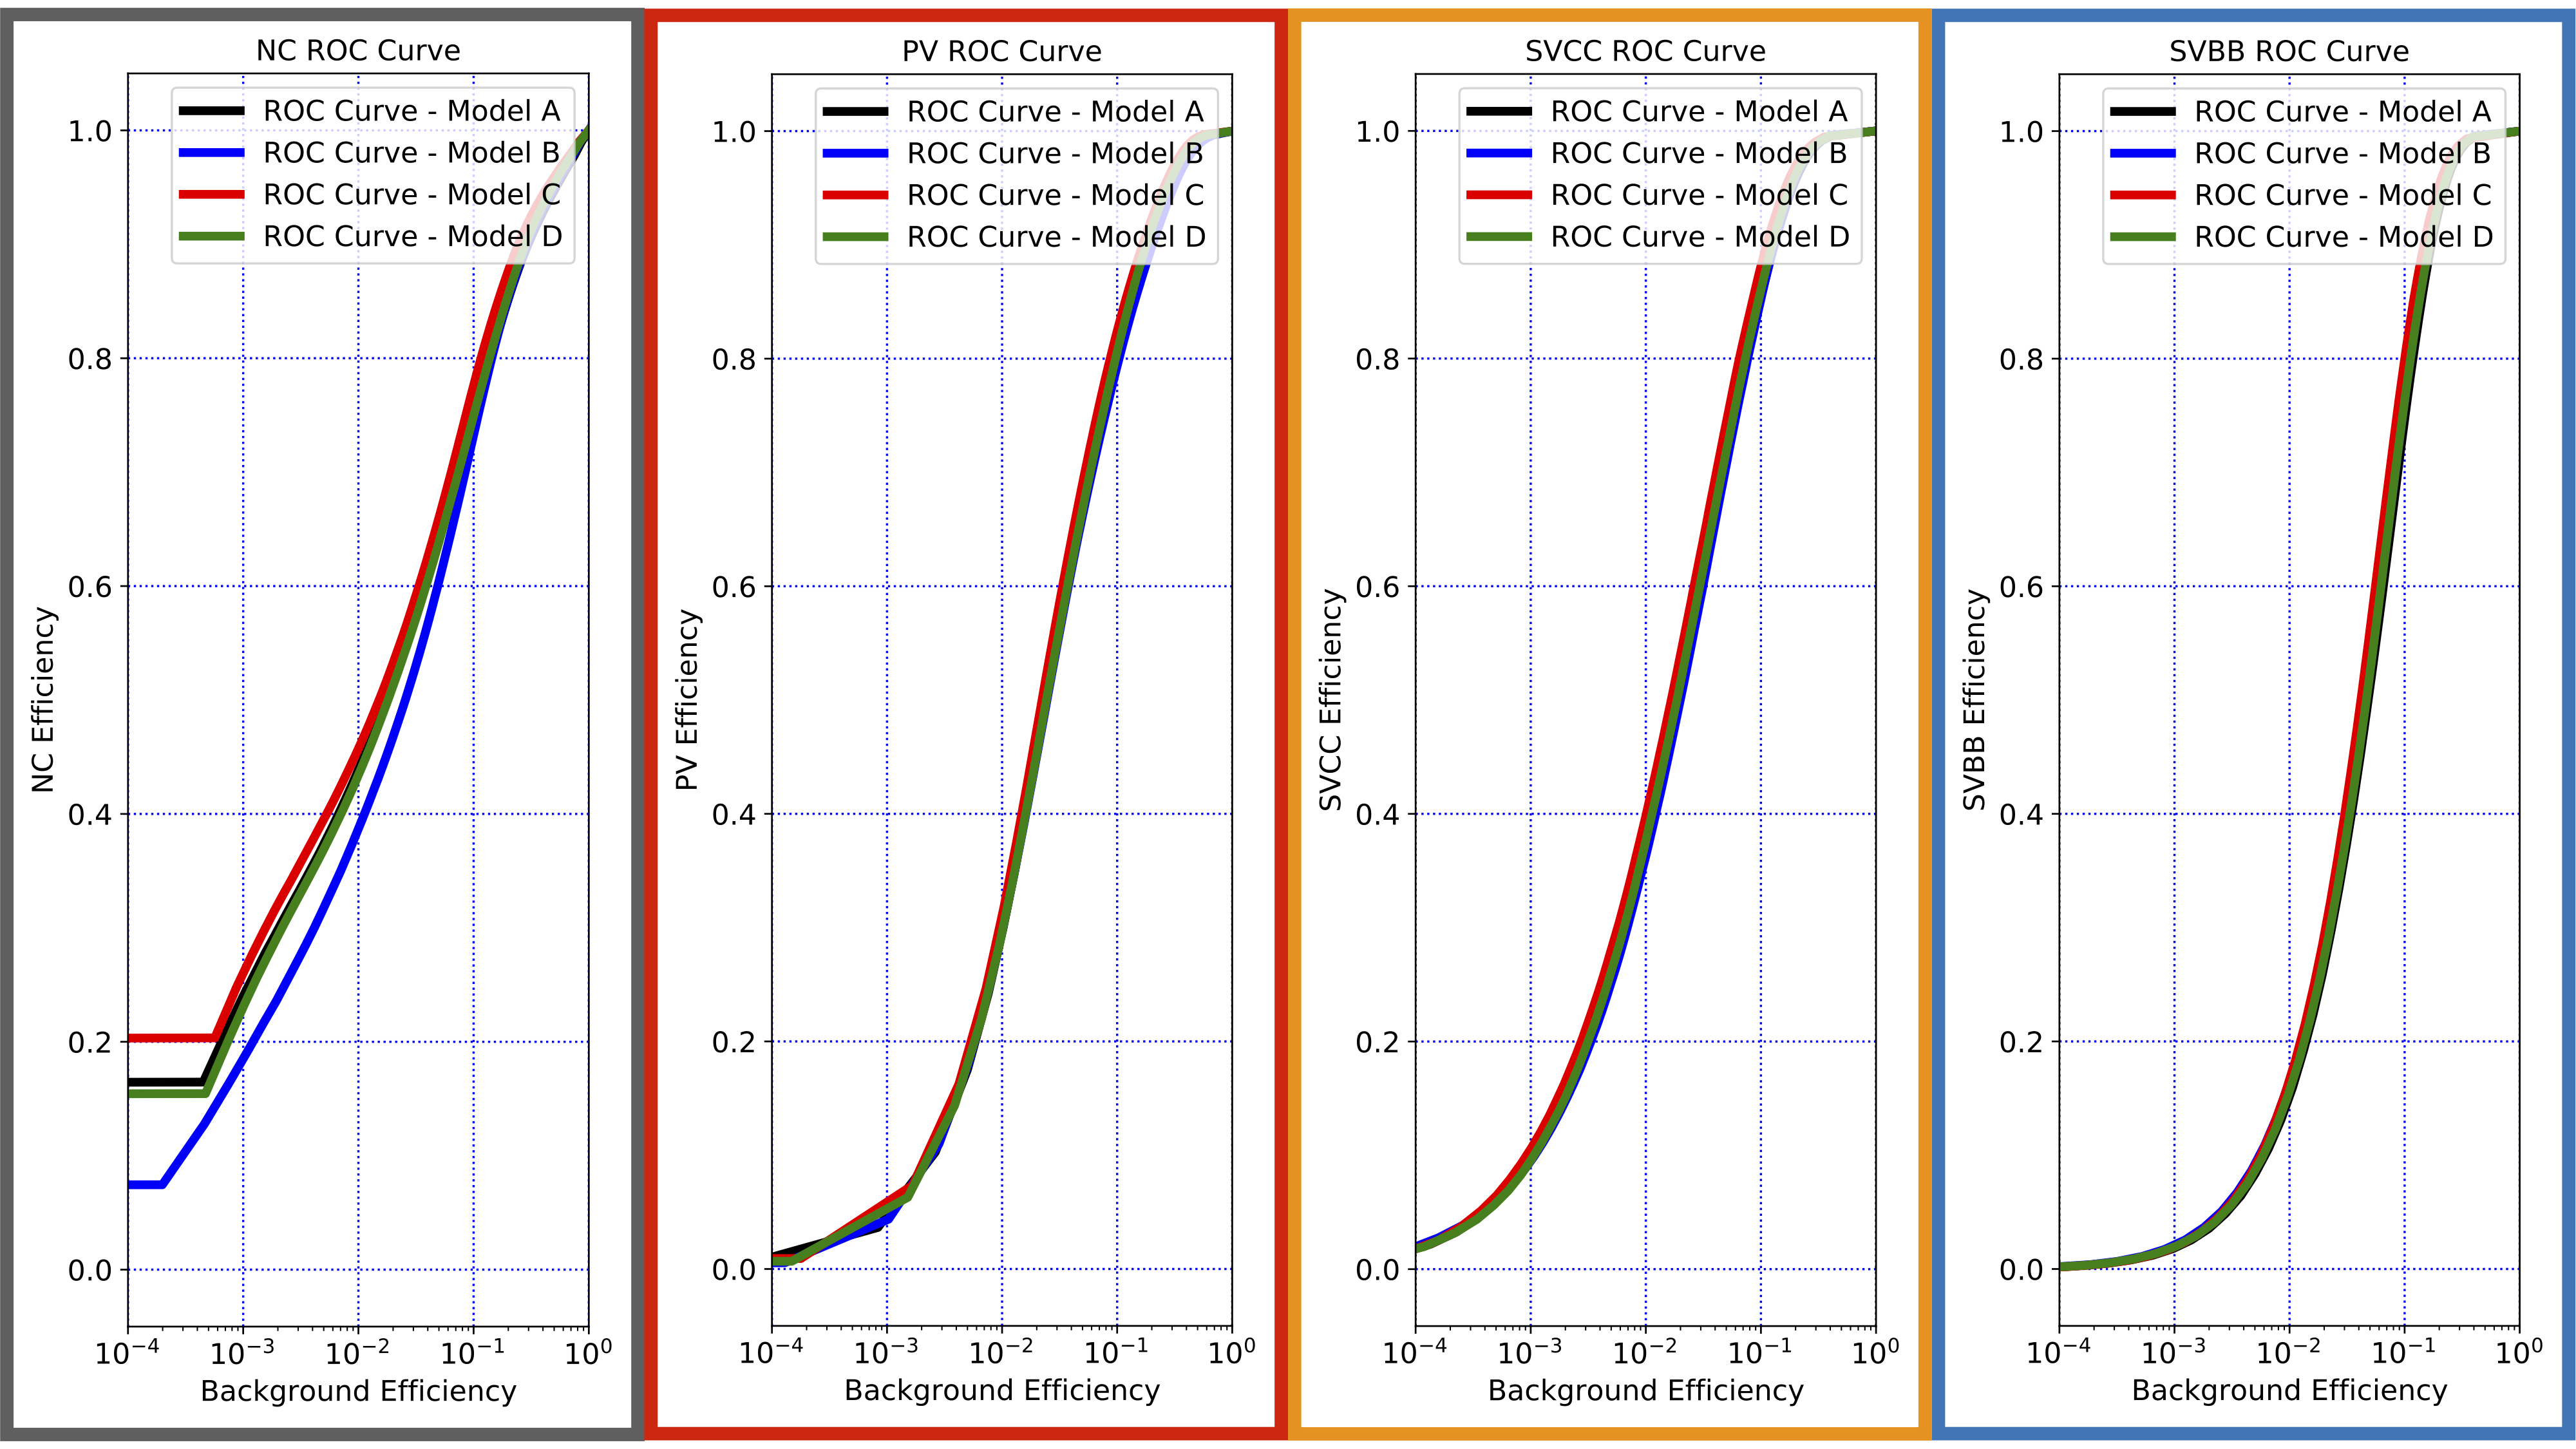
\includegraphics[width=1.0\textwidth, clip]{Figure/3Networks/3-3-3-2ROC_Curve_1.png}
   \end{minipage}
   
   \begin{minipage}{1.0\textwidth}
   \centering
    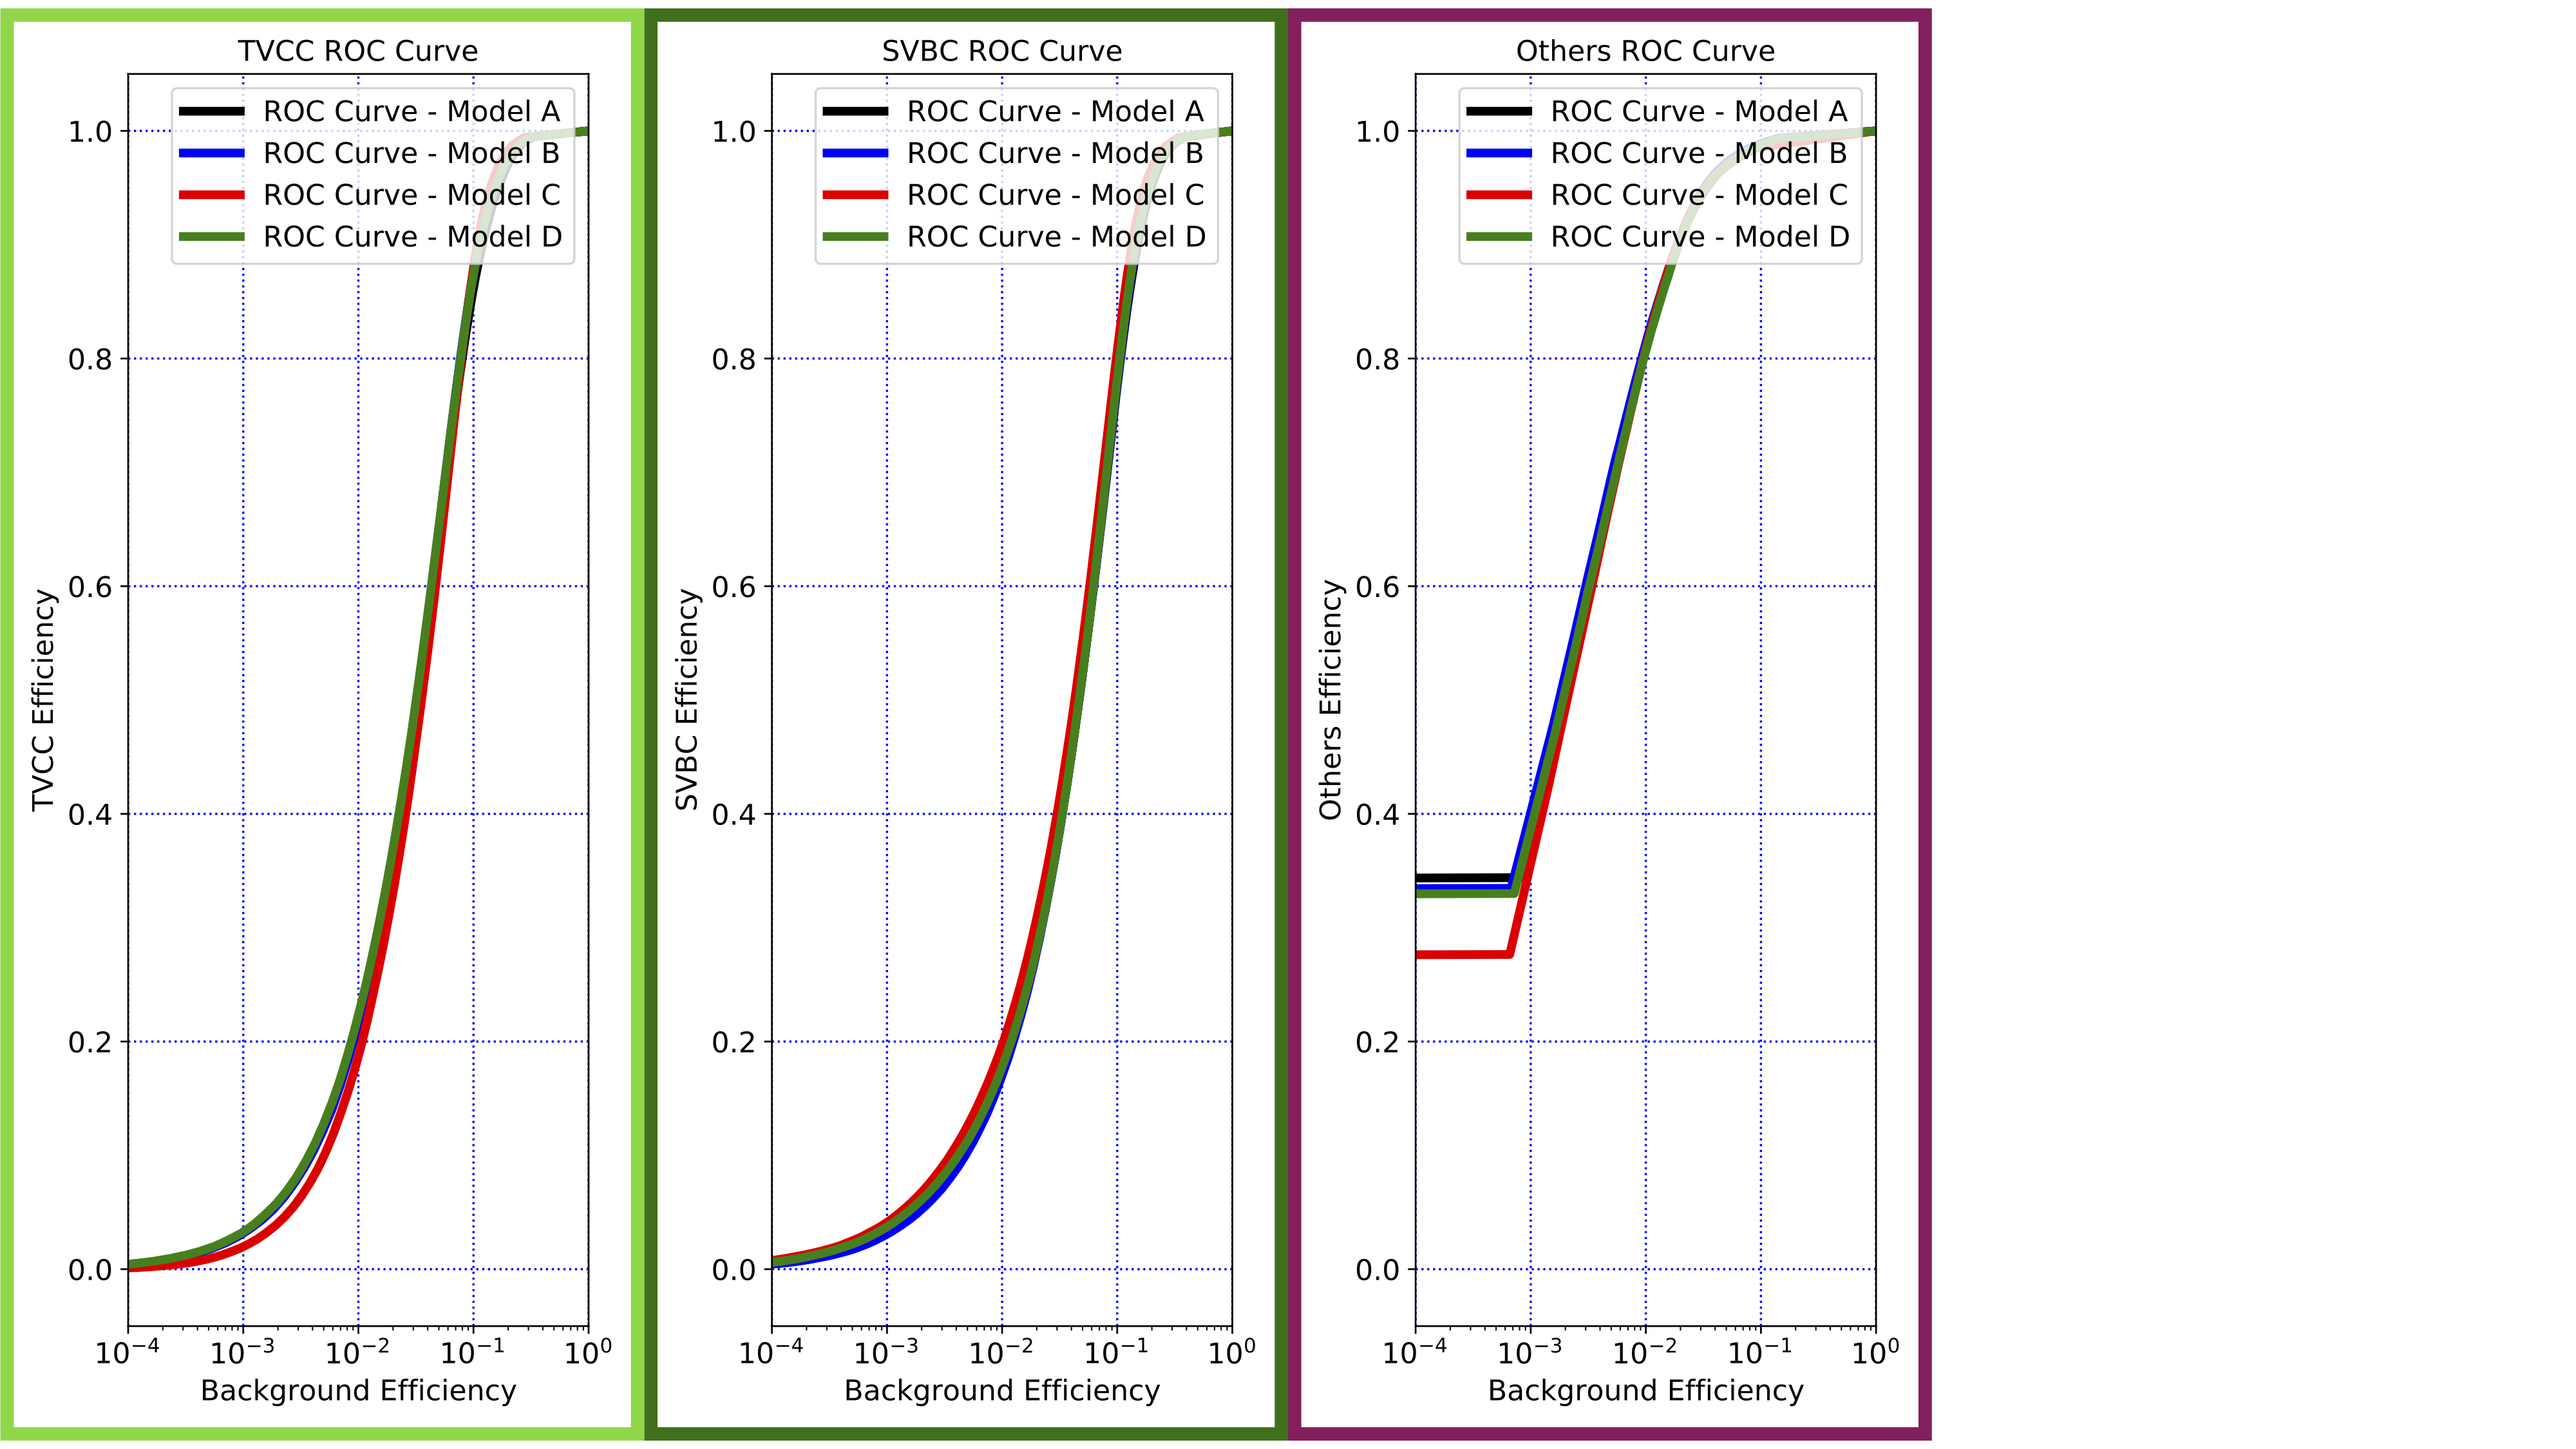
\includegraphics[width=1.0\textwidth, clip]{Figure/3Networks/3-3-3-2ROC_Curve_2.png}
   \end{minipage}
  \caption[各モデルのROC曲線]{各モデルのROC曲線。縦軸は信号効率、横軸はバックグラウンド効率である。黒線はモデルA、青線はモデルB、赤線はモデルC、緑線はモデルDをそれぞれ表している。}
  \label{3-3-3-2ROC_Curve}
 %\end{tabular}
\end{figure}

ネットワークがどの程度の効率や純度でクラスを分類出来ているかを更に把握するため混合行列を用いる(図\ref{3-3-3-2ConfusionMatrix})。
混合行列は横軸をネットワークによって予想されたクラス、縦軸を正解ラベルでのクラスとしてデータを行列化したものである。
したがって、対角成分が正答、それ以外は誤答である。
ここでは、効率について規格化したものと純度について規格化したものの二つで評価を行う。
また、比較のためモデルB,C,Dの結果についてはモデルAとの相対値で表している。

\begin{figure}[htbp]
 \centering
  %\begin{tabular}{cccc}
  \begin{minipage}{1.0\textwidth}
   \centering
    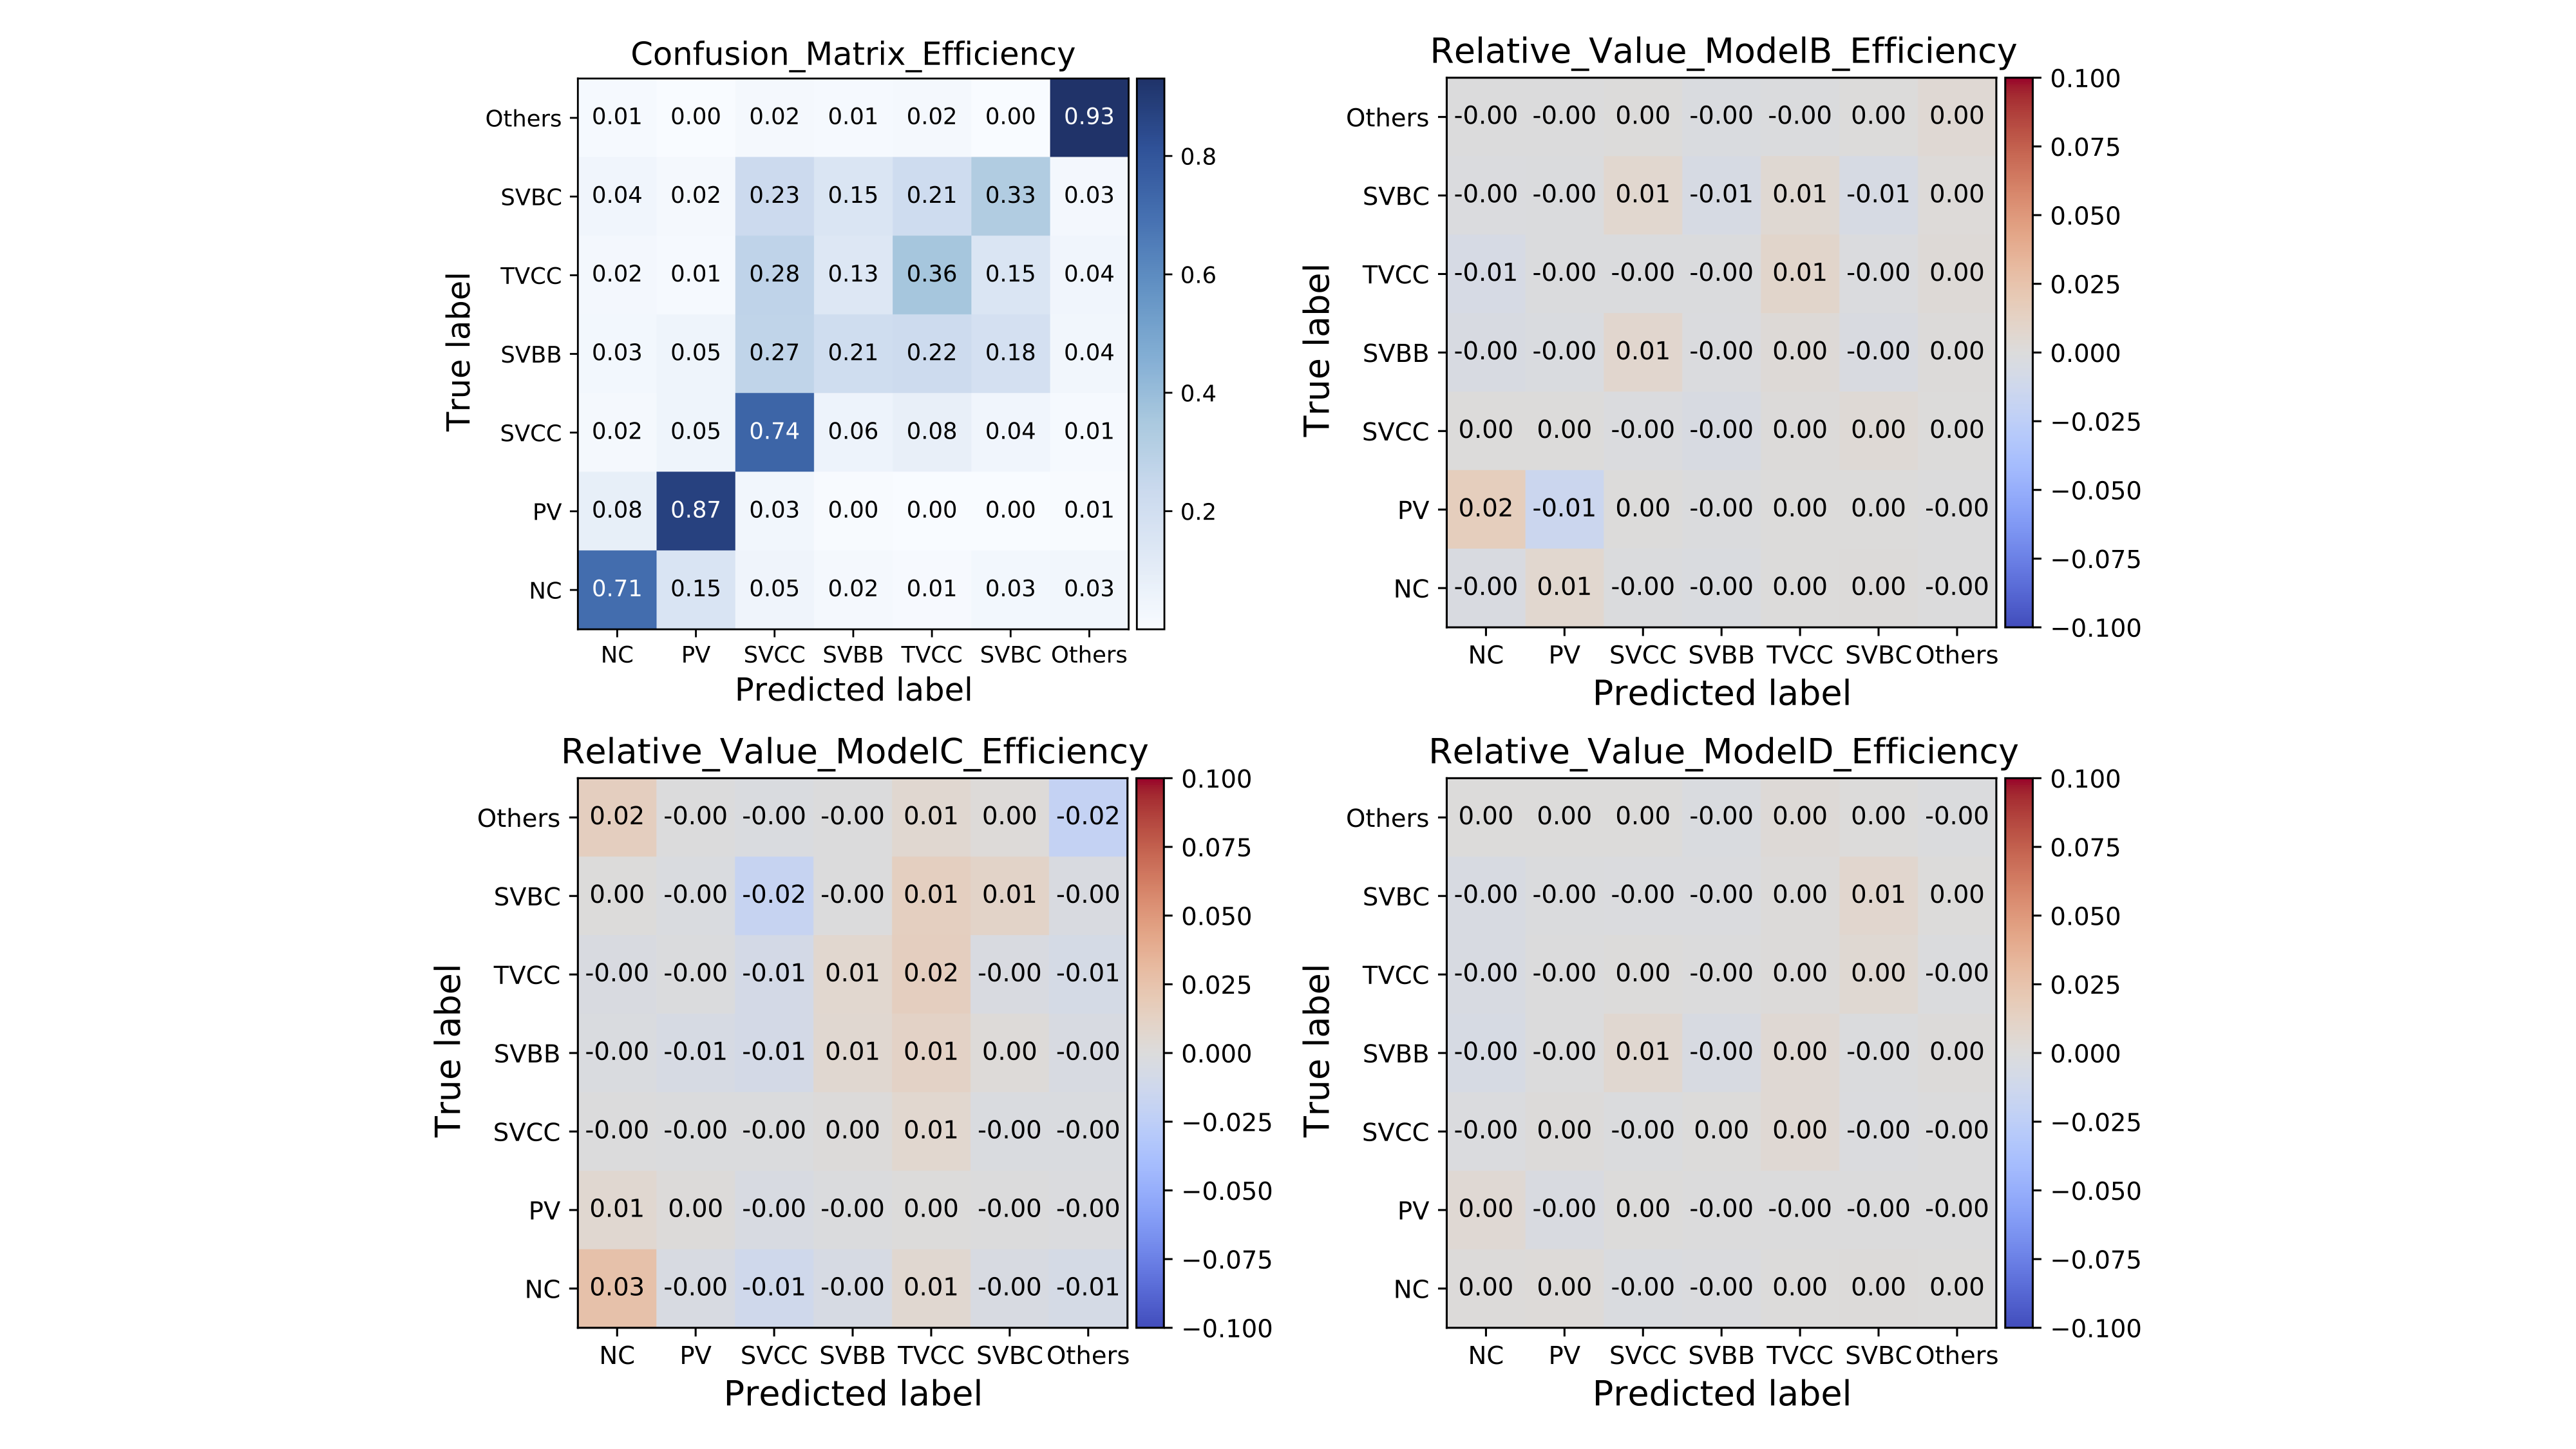
\includegraphics[trim = 300 0 300 0, width=0.9\textwidth, clip]{Figure/3Networks/3-3-3-2ConfusionMatrix_1.png}
   \end{minipage}
   
   \begin{minipage}{1.0\textwidth}
   \centering
    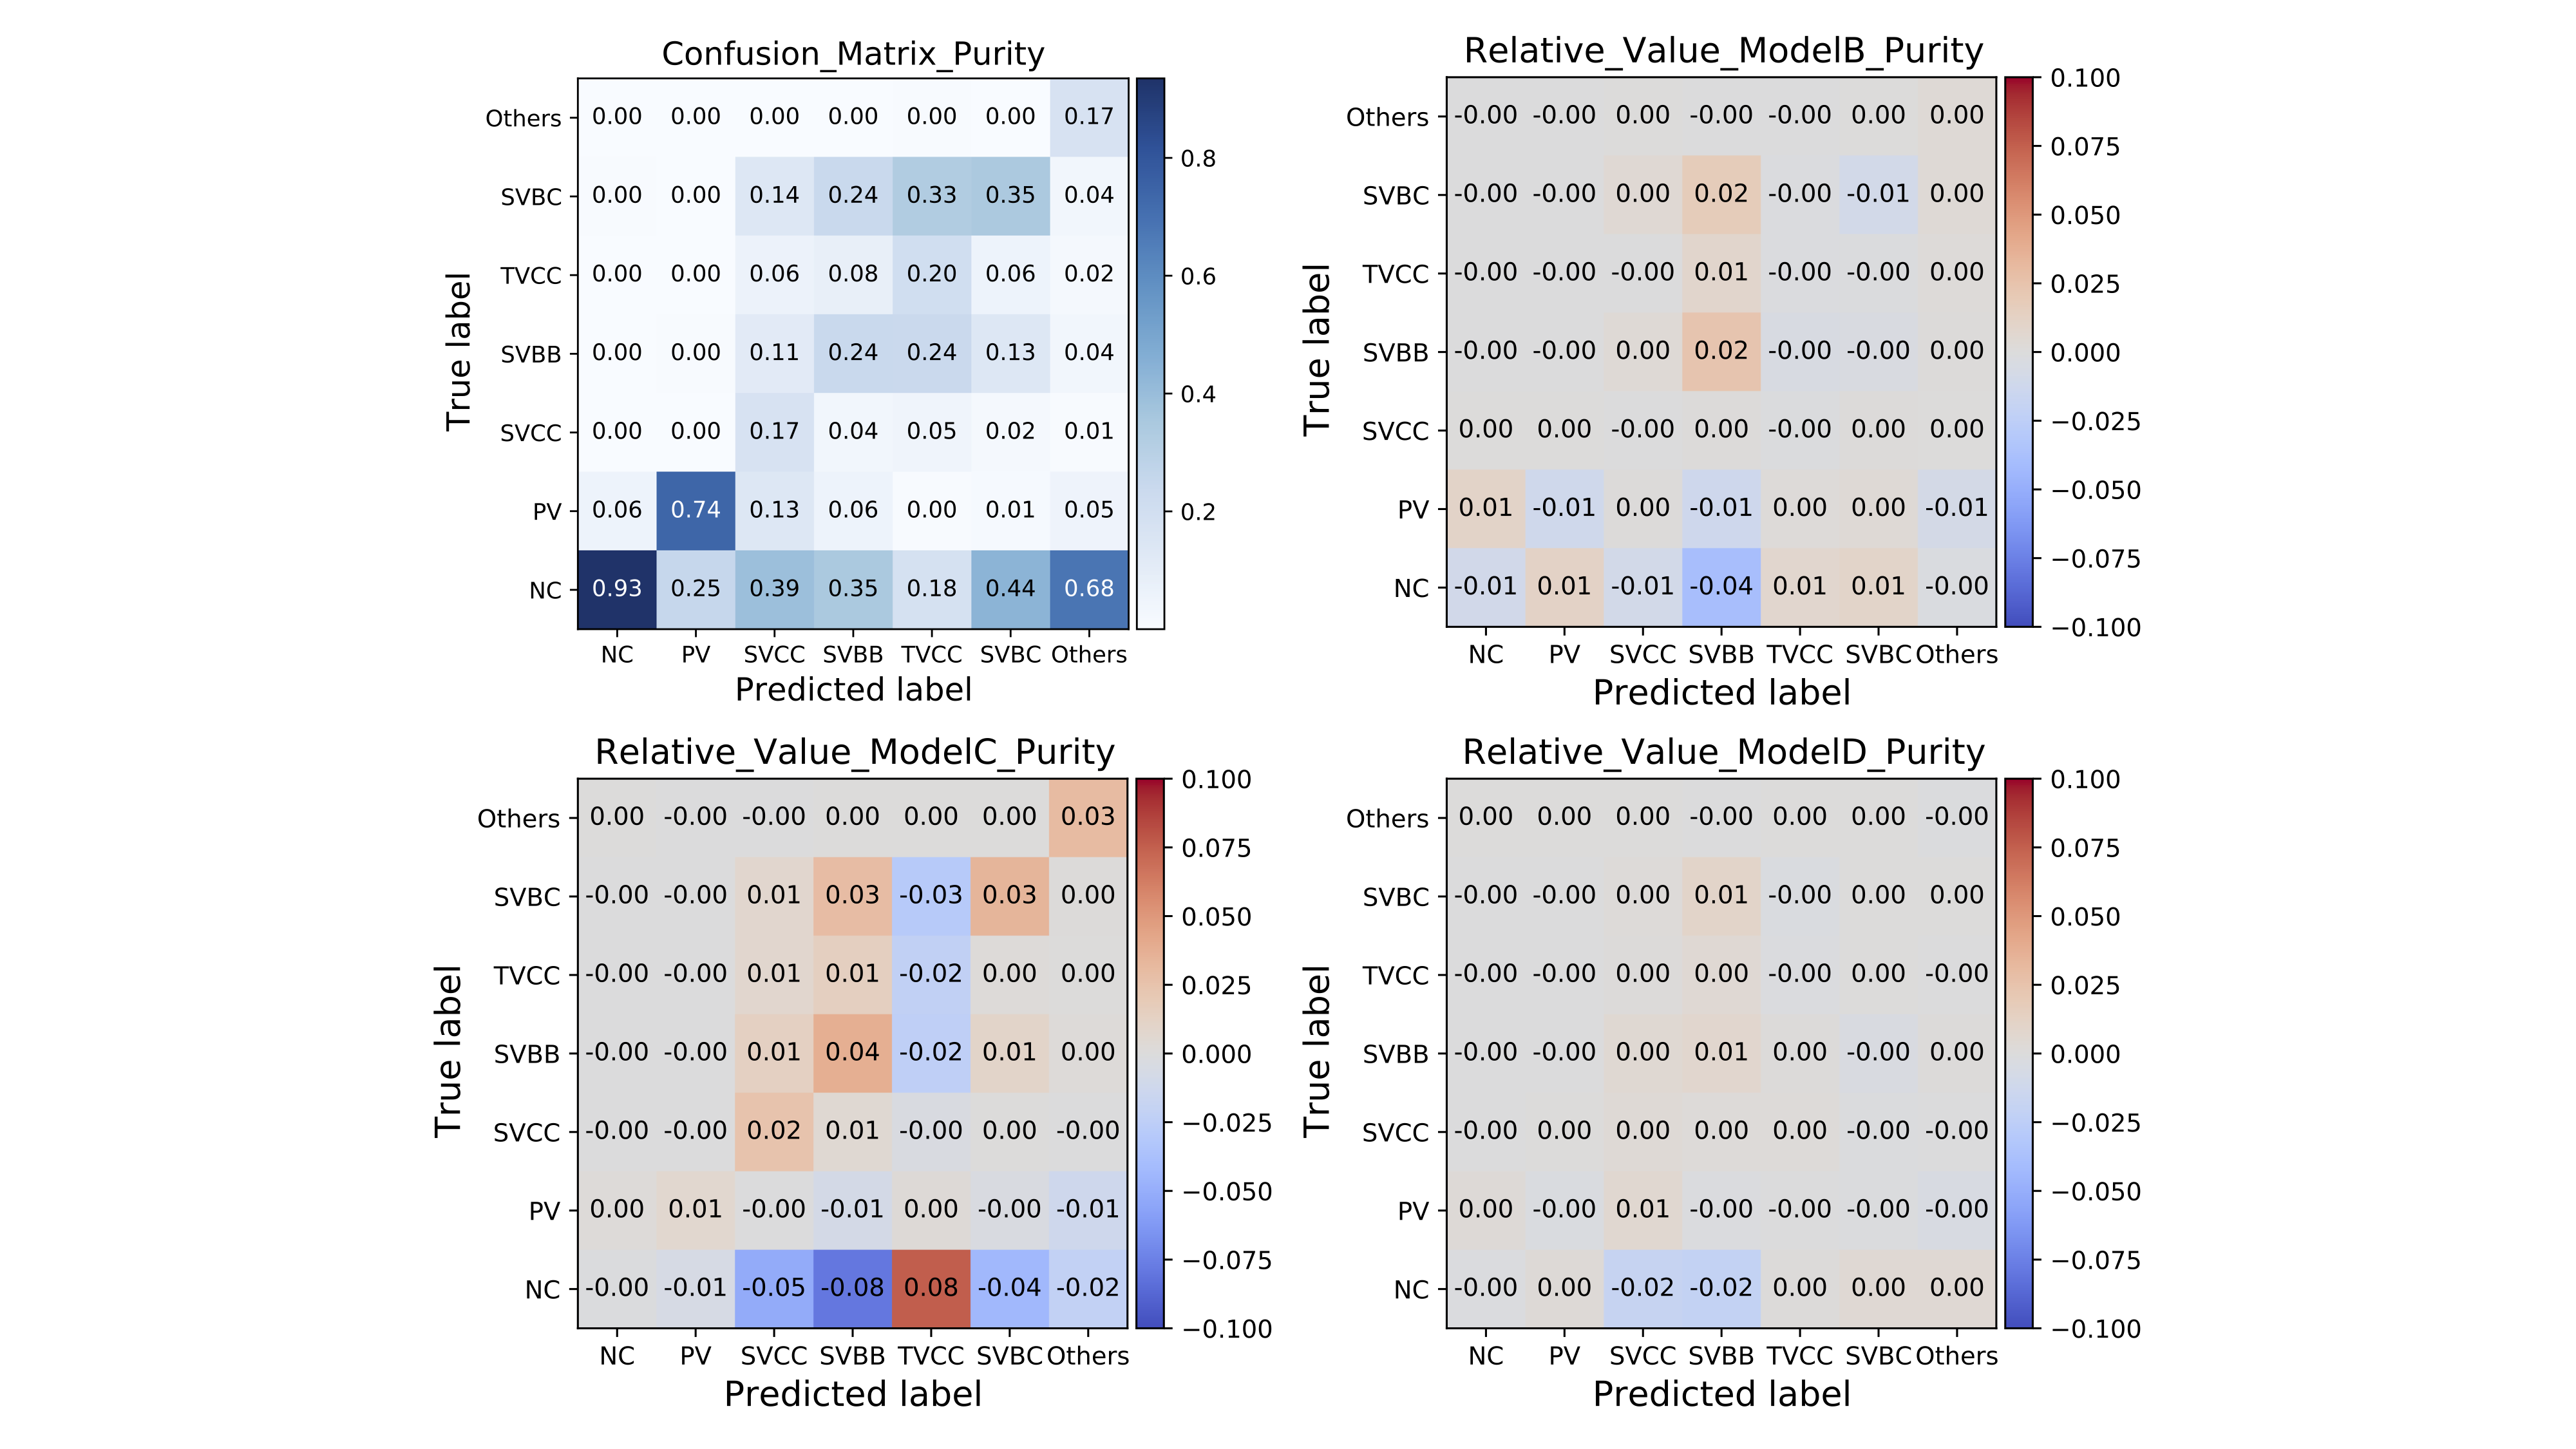
\includegraphics[trim = 300 0 300 0, width=0.9\textwidth, clip]{Figure/3Networks/3-3-3-2ConfusionMatrix_2.png}
   \end{minipage}
  \caption[各モデルの混合行列と各モデルの相対値]{各モデルの混合行列と各モデルの相対値。図上部は効率について規格化、図下部は純度について規格化した行列である。それぞれ左上がモデルA、右上がモデルB、左下がモデルC、右下がモデルDの結果である。モデルB・C・Dに関してはモデルAとの相対値で表現している。}
  \label{3-3-3-2ConfusionMatrix}
 %\end{tabular}
\end{figure}

図上部は効率について規格化したものである。
そのため正解ラベル方向 (行方向) の和が1になっている。
混合行列では、NP・PV・SVCC・Othersが比較的高い効率で分離できていることが分かる。
一方、各SVについては殆ど分離できておらす、個々のフレーバーや準崩壊点などは区別できていない。
ただし、SVとそれ以外との分離は実現できており、SVであることは識別できているが、それがSVのどの崩壊点の種類であるかという点については識別が不十分となっている。

図下部は純度について規格化したものである。
そのため予想されたクラス方向 (列方向) の和が1になっている。
純度については不均衡データとしての特性が強調され、図\ref{3-3-2-2ImbalancedData}のようなNCやPVが支配的なクラス配分となっていることから、各SVに対してのNCからの汚染が顕著である。
ただし、これは後述する\ref{VFDL:TuneandPerformanceofVFDL}節での崩壊点のタネの選別によってある程度の軽減が可能である。

相対値では対角成分が正であれば性能が高い、それ以外の成分が正であれば性能が低いと判断できる。
ModelA・B・Dについてはあまり変化はなく、殆どの差異は$0$~$2$\%程度に収まっている。
ModelCについても同様に大きな違いは確認できないが、効率について規格化した混合行列内のSVBB・TVCC・SVBCの分類性能が向上しており、かつ純度について規格化した混合行列内のNCからのSVCC・SVBB・SVBCへの流入がある程度減少している。
ここで、TVCCへの流入しついては大幅に増大しているが、これはTVCCへの他のSVからの流入が少なくなったことによって相対的に上昇している為であると考えられる。

以上のことから、ネットワークはNC・PV・Othersや単にSVとしては大まかにクラス分類ができていると分かる。
また、位置に関してもある程度の予想ができていると考えられる(図\ref{})。
一方、SV内の各崩壊点の種類への分離は困難でありModelCで多少の改善が見られることから、詳細な位置の再構成には至っておらず、SV内の分離に関しては更なる情報の入力、もしくは抜本的なネットワーク構造の改良が必要であると考えられる。\\

2. t-SNEによるネットワークの理解\\

深層学習のネットワーク内部を理解することは非常に難しい課題の一つである。
ネットワークが何故、どのようにクラス分類を決定したかを把握する事は容易ではないが、どの程度各クラスを分離して判断できているかは次元削減によってある程度理解が可能である。
ここでは、t-SNEという手法を用いて次元削減を行った。

t-SNEとは、高次元の情報についての距離関係を維持しつつ、低次元へマッピングするアルゴリズムである。
データの局所的な構造や非線形の次元削減が可能であり、ここではネットワークがどの程度各クラスを分離できているかを二次元の画像として把握することができる。

そのような結果を図\ref{3-3-3-3tSNE}に示す。
入力変数では殆ど分離できていなかった各クラスが、出力層の直前ではある程度分離できている事が確認できる。
また、各SVは非常に近い位置にマップされており、分離が困難であると分かる。
更に、分布は線対称な形をしており、これは二本の飛跡についての情報を十分に混合できていないということを意味していると考えられる。

\begin{figure}[htbp]
 \centering
 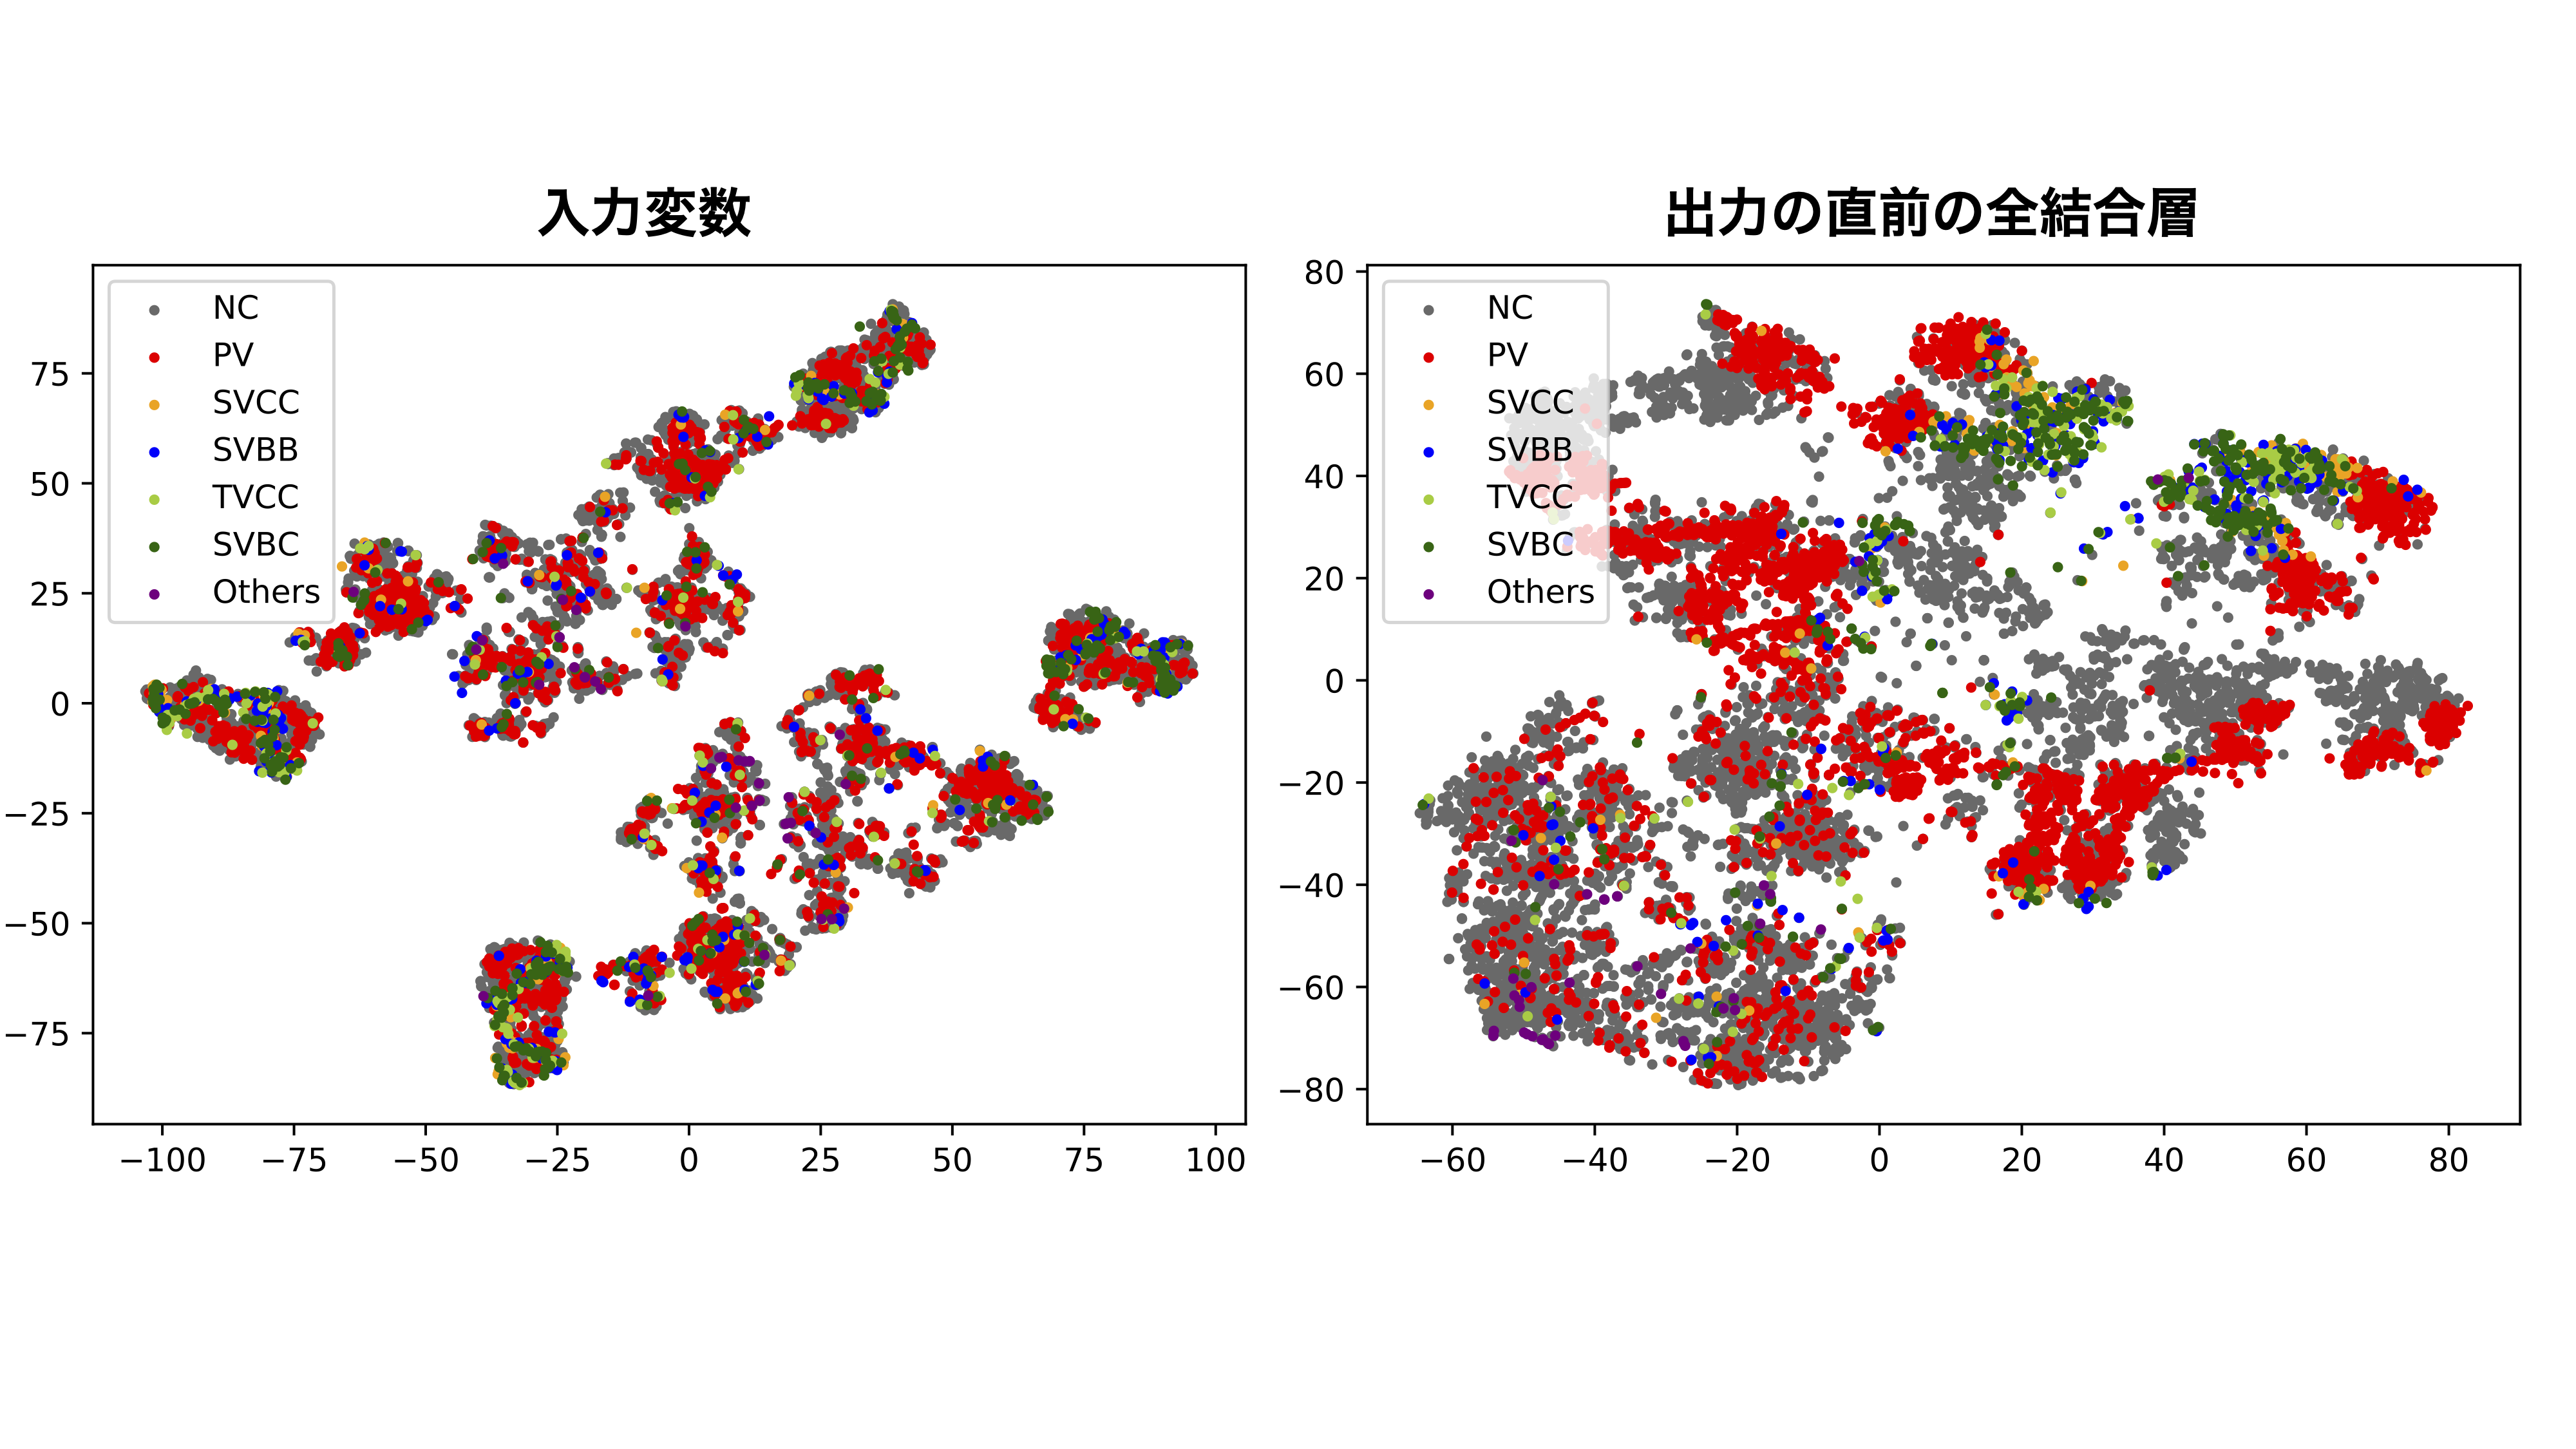
\includegraphics[width=1.0\textwidth]{Figure/3Networks/3-3-3-3tSNE.png}
 \caption[t-SNEによる次元削減の比較]{t-SNEによる次元削減の比較。左図は入力変数 ($22$変数) を二次元に削減したもの、右図は分類問題への分離の直前の全結合層 ($256$変数) を二次元に削減したものである。}
 \label{3-3-3-3tSNE}
\end{figure}


%%%%%%%%%%%%%%%%%%%%%%%%%%%%%%%%%%%%%%%%%%%%%%%%%%%%%%%%%%%%%%%%%%%%%%%%%%%%%%%%%%%%%%%%%%%%%%%%%%%%%
\section{任意の数の飛跡についてのネットワーク} \label{Net:VertexLSTM}

ここでは\ref{Net:forVertexFinderwithDL}節で紹介した二つのネットワークの内、任意の数の飛跡についてのネットワークに関して述べる。
前節と同様にネットワークの構造・学習・評価について\ref{Net:VLSTM:StructureofVLSTM}項・\ref{Net:VLSTM:TrainingandStrategyofVLSTM}項・\ref{Net:VLSTM:PerformanceofVLSTM}項でそれぞれ解説する。

任意の数の飛跡についてのネットワークは、崩壊点を生成するためのネットワークである。
ここでは、リカレントニューラルネットワークの初期状態として飛跡対 (崩壊点のタネ) を入力し、系列データとして事象中の全ての飛跡を入力する。
また出力の作り方はMany to Manyとし、事象中のそれぞれの飛跡が初期状態の崩壊点のタネに対して結合しているか否かを評価するネットワークを構築する。

\begin{figure}[htbp]
 \centering
 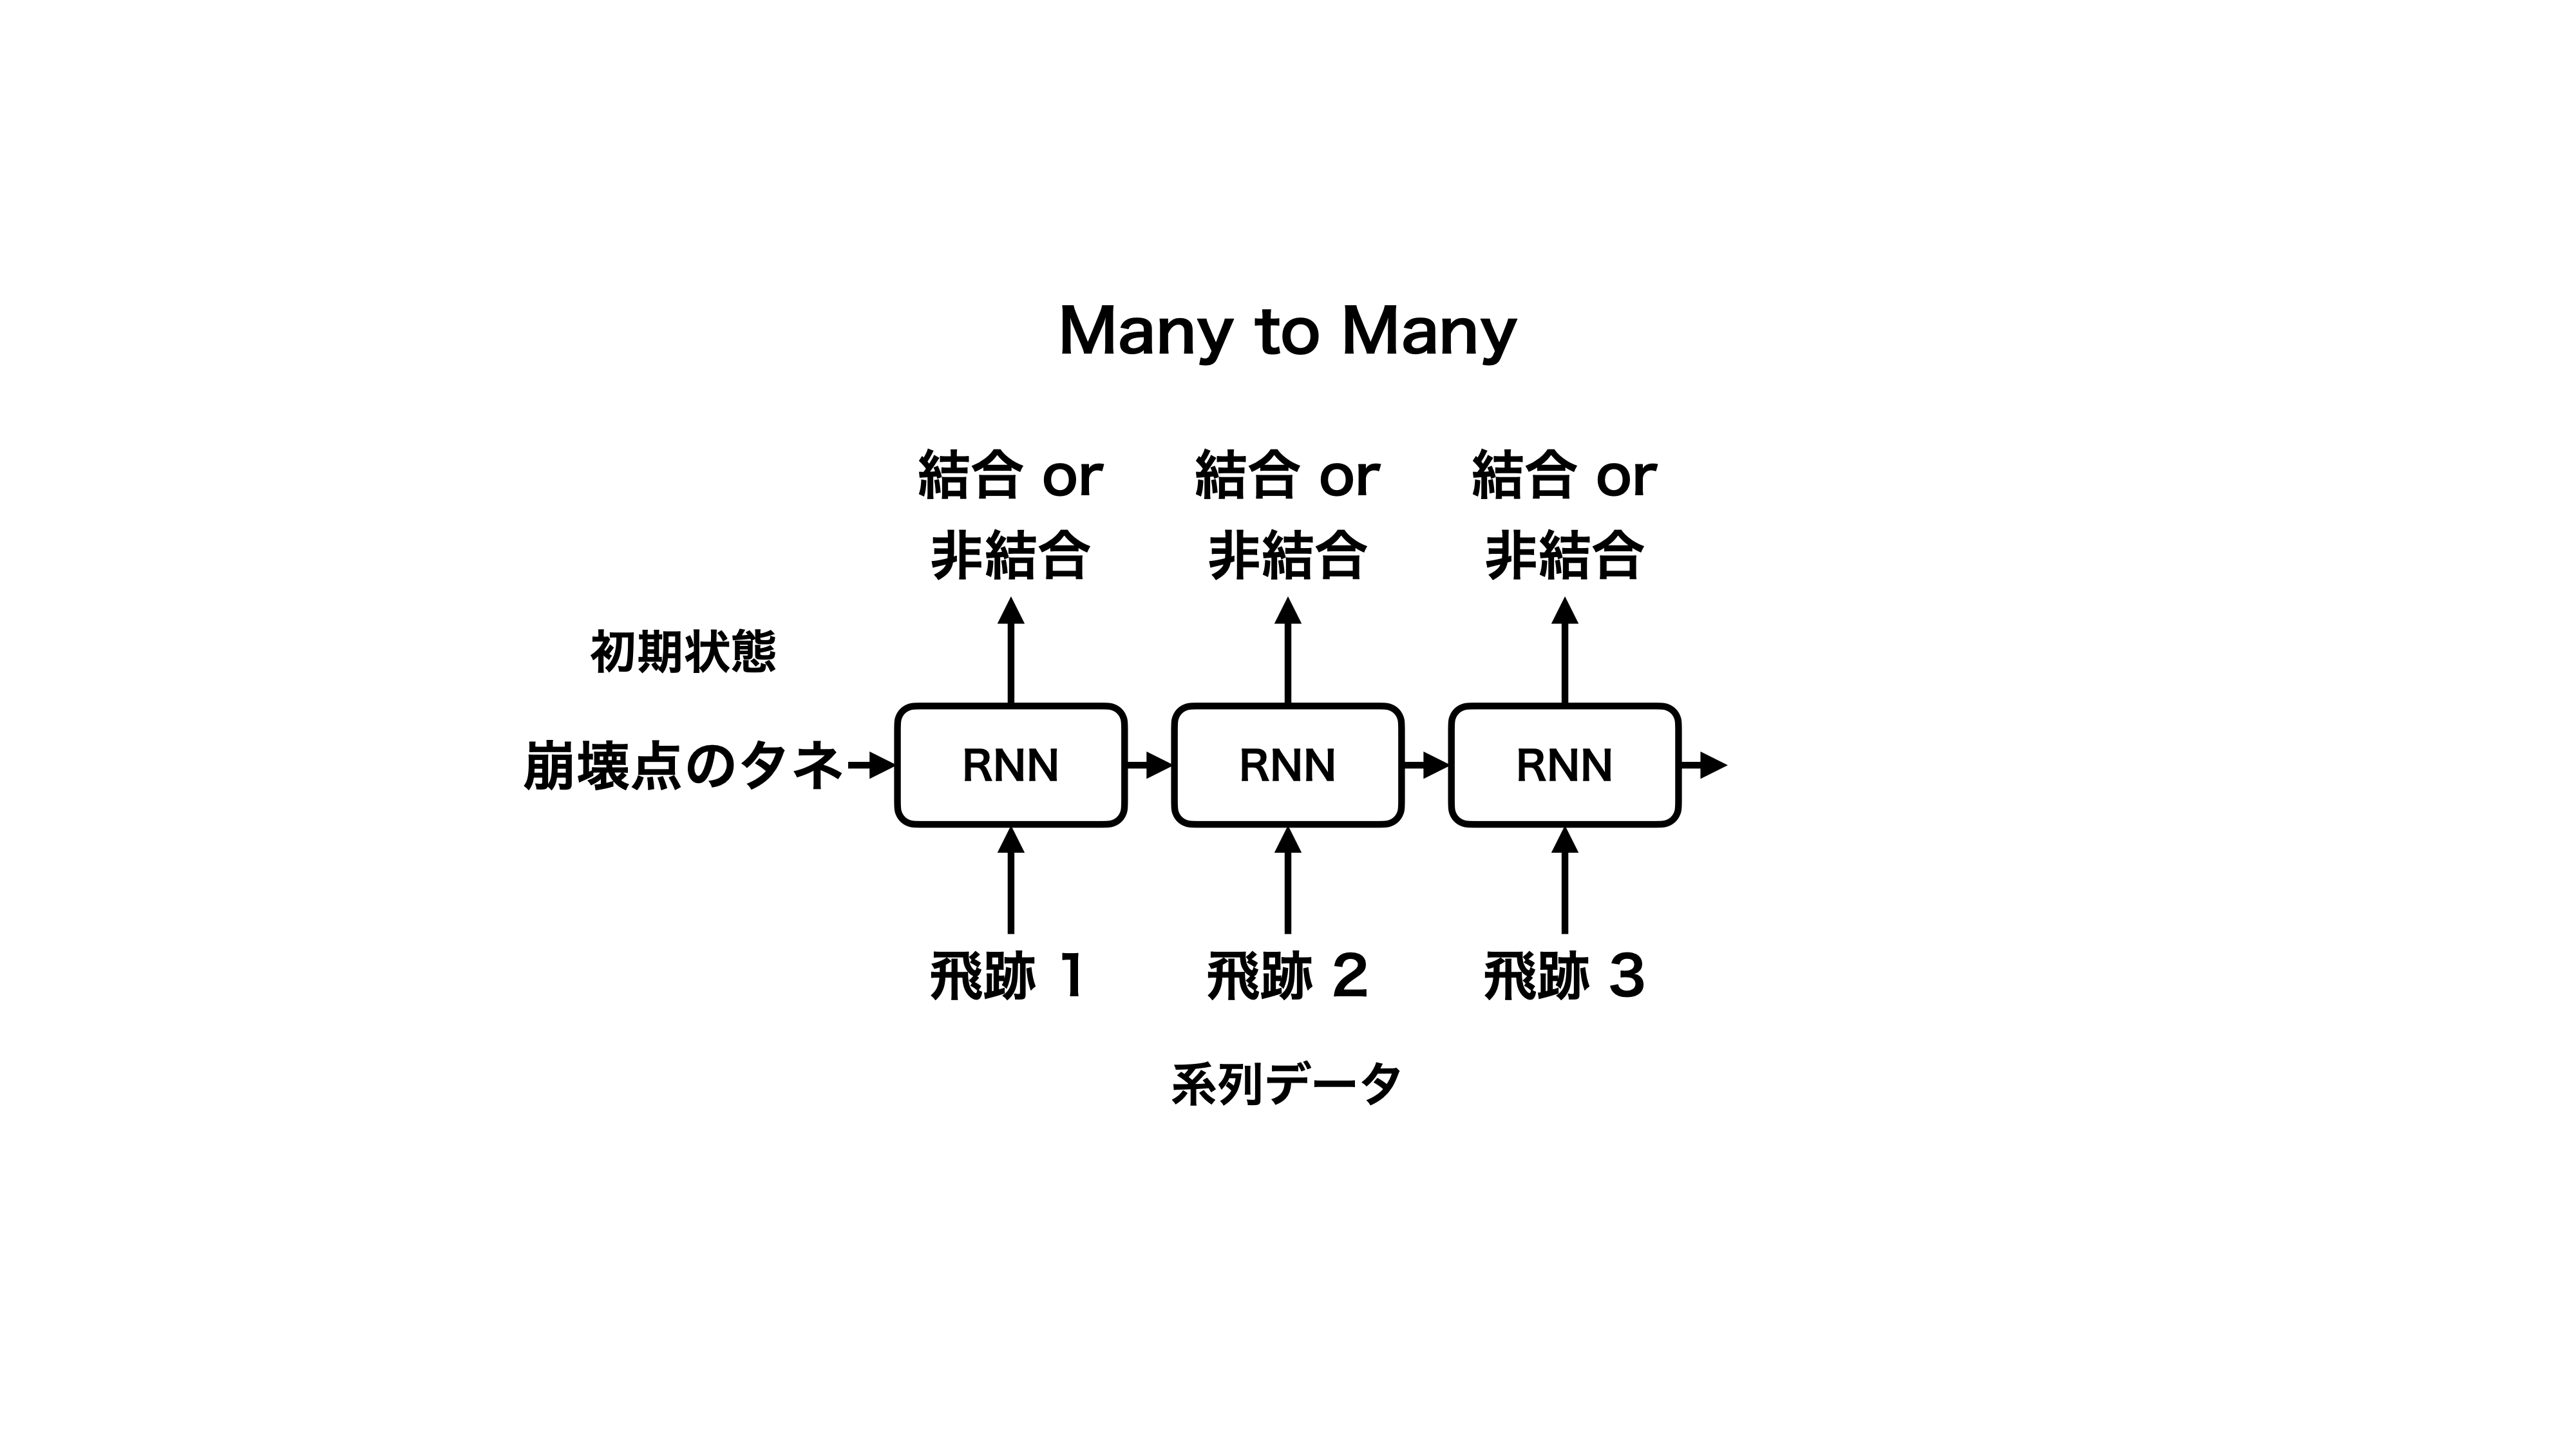
\includegraphics[trim = 200 150 200 150, width=0.9\textwidth, clip]{Figure/3Networks/3-4-0-1VertexProductionwithRNN.png}
 \caption[リカレントニューラルネットワークを用いた崩壊点生成]{リカレントニューラルネットワークを用いた崩壊点生成。初期状態として崩壊点のタネを入力し、系列データとして事象中の飛跡を入力している。事象中の飛跡はそれぞれ一本ずつ評価され、出力はそれらの飛跡が初期状態の崩壊点のタネと結合しているか、非結合であるかである。}
 \label{3-4-0-1VertexProductionwithRNN}
\end{figure}


%%%%%%%%%%%%%%%%%%%%%%%%%%%%%%%%%%%%%%%%%%%%%%%%%%%%%%%%%%%%%%%%%%%%%%%%
\subsection{ネットワークの構造} \label{Net:VLSTM:StructureofVLSTM}

まず、任意の数の飛跡についてのネットワークとして図\ref{3-4-1-1SimpleVLSTM}のようなネットワークを考える。

\begin{figure}[htbp]
 \centering
 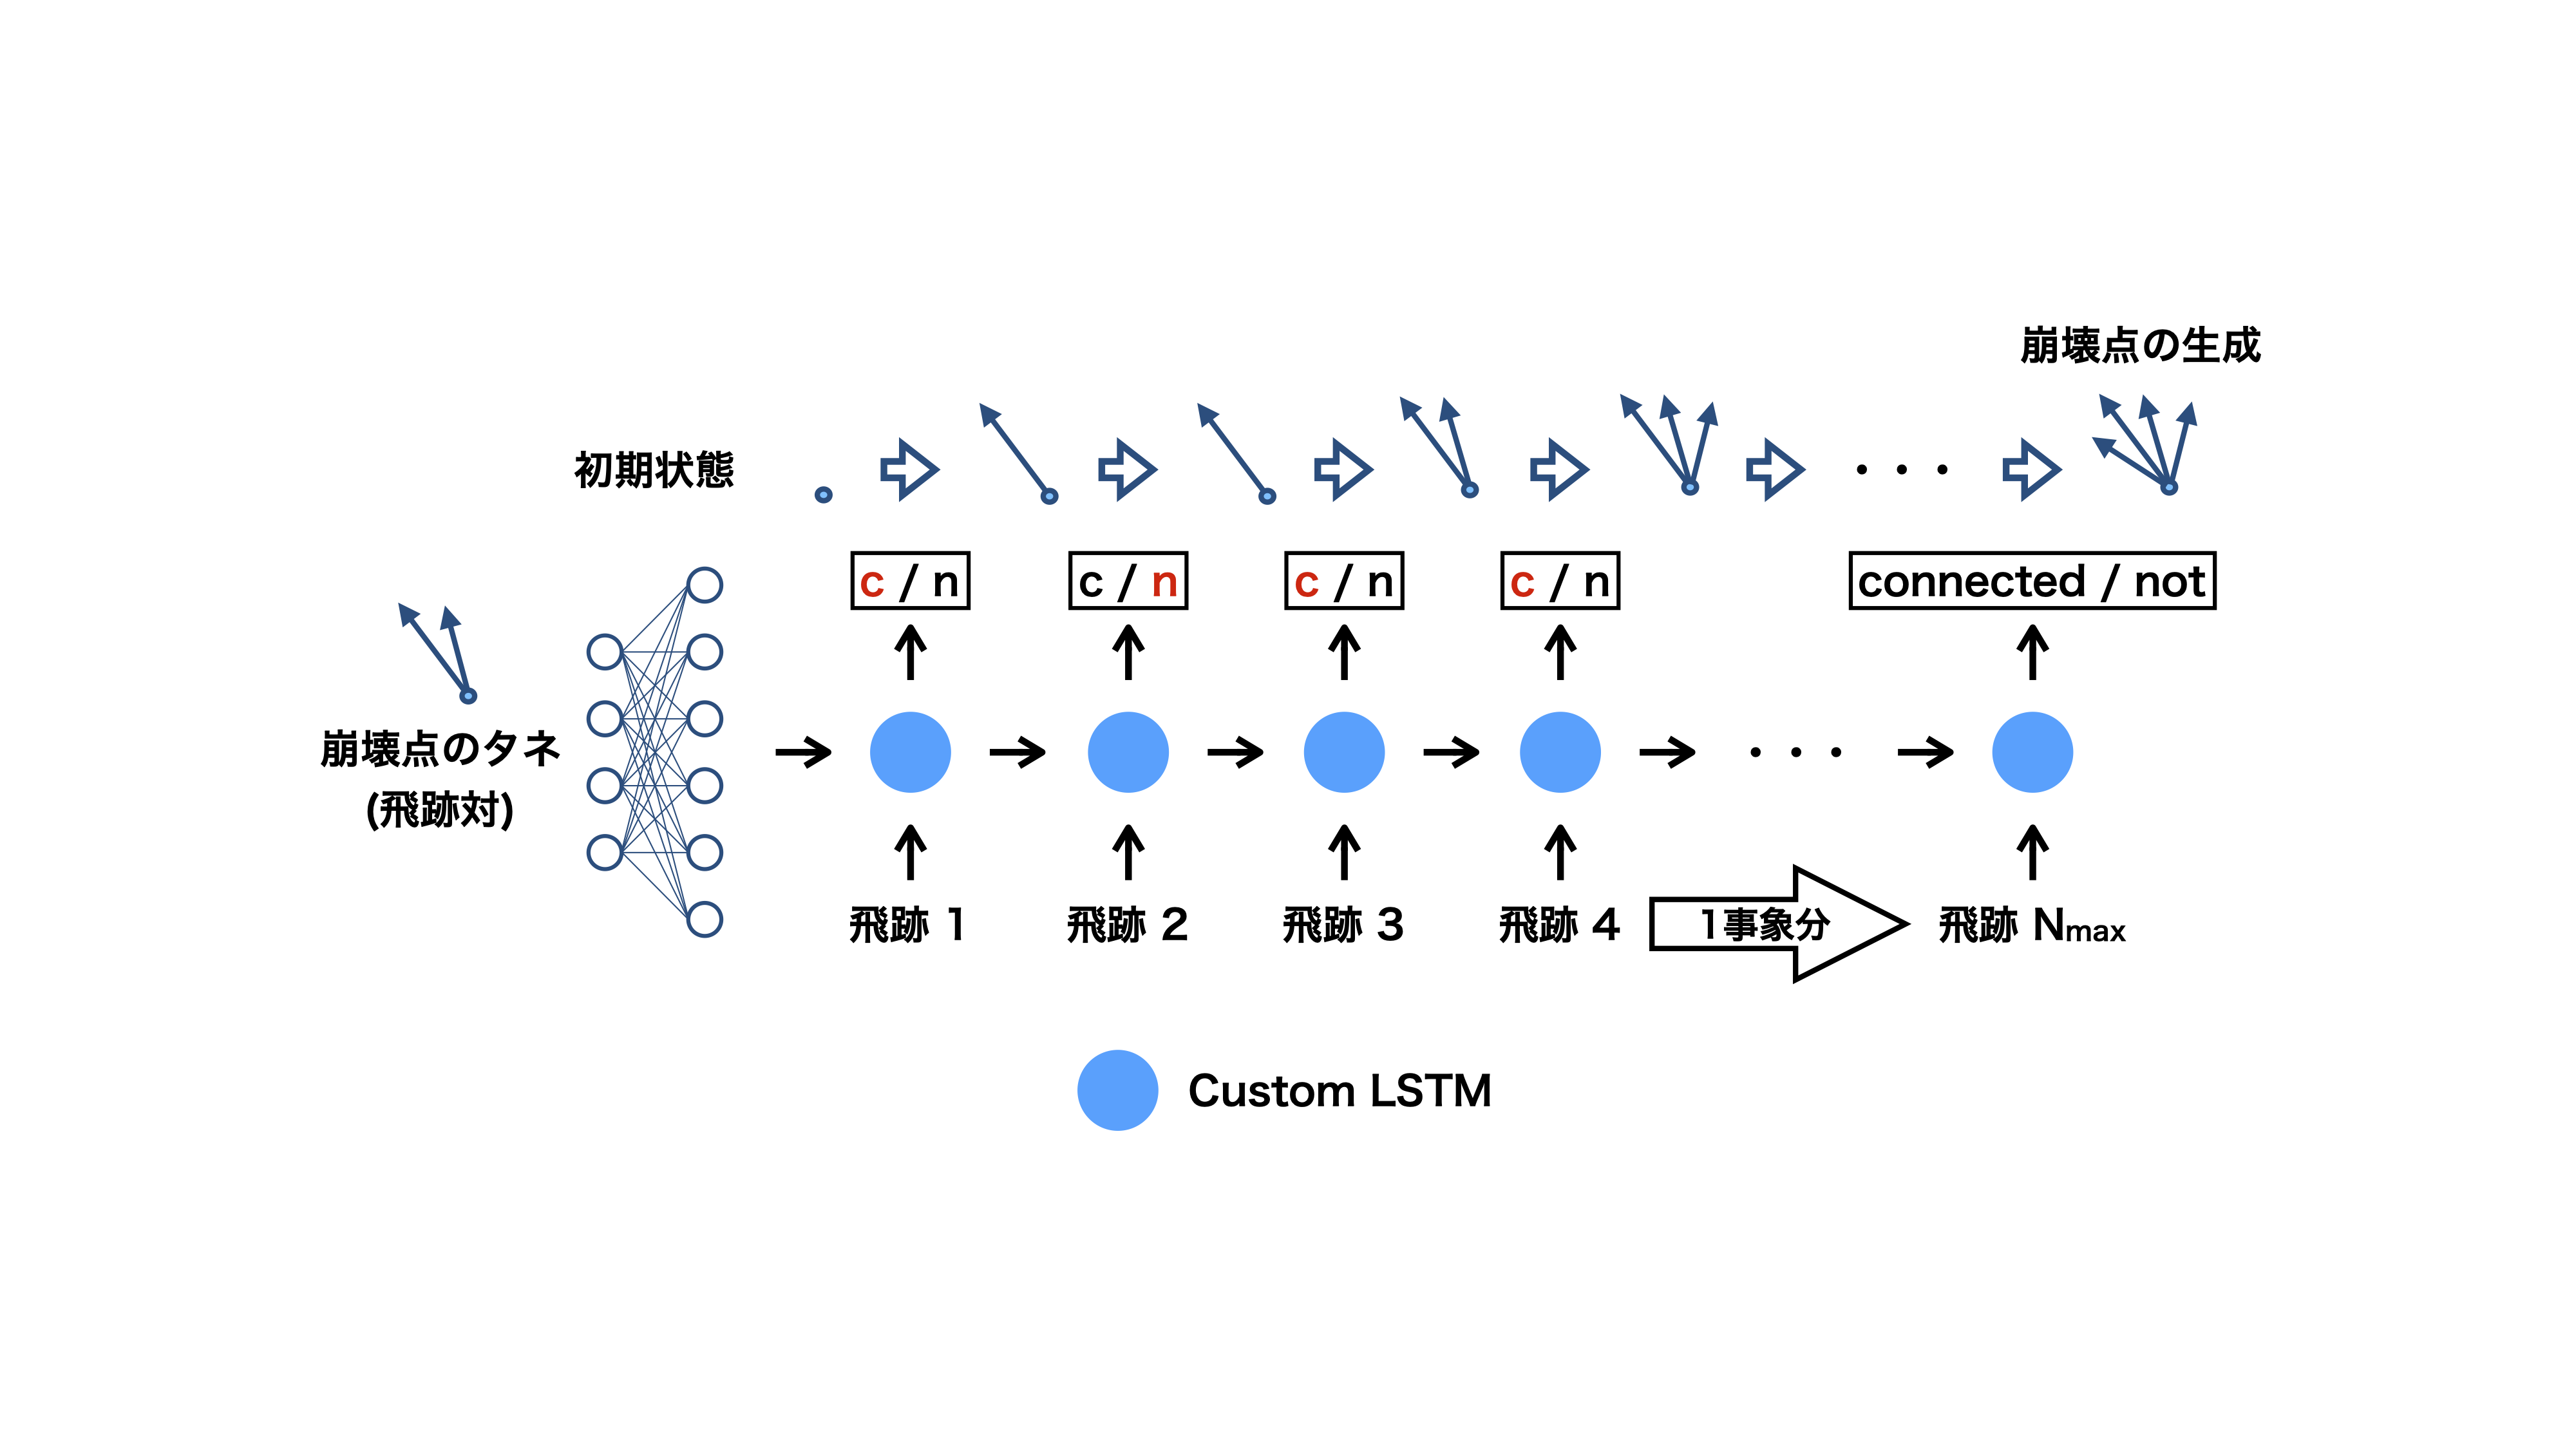
\includegraphics[trim = 100 200 100 200, width=1.0\textwidth, clip]{Figure/3Networks/3-4-1-1SimpleVLSTM.png}
 \caption[崩壊点生成のためのリカレントニューラルネットワーク構造]{崩壊点生成のためのリカレントニューラルネットワーク構造。図上部で崩壊点の生成の様子を図示した。飛跡がタネに結合していれば隠れ状態は逐次的に更新されていき、事象中の全ての飛跡を評価した段階で崩壊点が生成される。実際には系列データとして入力される飛跡に関しても、全結合層を用いてEmbeddingを行い抽象化している。}
 \label{3-4-1-1SimpleVLSTM}
\end{figure}

前述したように崩壊点のタネを初期状態として使用している。
実際には崩壊点のタネは飛跡二本分の情報 ($44$個の変数) であり、更に全結合層を介してより抽象的な崩壊点の情報を初期状態として入力できるようにしている。
また系列データとして事象中の全ての飛跡を用いている。
出力はこの飛跡のそれぞれが崩壊点のタネと結合しているか否かである。

\ref{DL:RNN:LongShortTermMemory}で解説したようにリカレントニューラルネットワークは系列情報を保持する為、直前の系列に依存するように設計されている。
しかし飛跡は本質的に順序を持っていないことに注意する必要がある。
図\ref{3-4-1-1SimpleVLSTM}では便宜的に飛跡について番号を振り表現しているが、これは人が決めた順序であり、本来、事象中の飛跡は系列データではない。
したがって、リカレントニューラルネットワークをそのまま用いることはデータの性質に合わない。
この為私は、リカレントニューラルネットワークの一つであるLSTMを拡張し、新しい独自のリカレントニューラルネットワークの構造を構築した。

図\ref{3-4-1-2VLSTMStructure}はそのような独自のリカレントニューラルネットワークについての1系列分のステップの詳細である。

\begin{figure}[htbp]
 \centering
 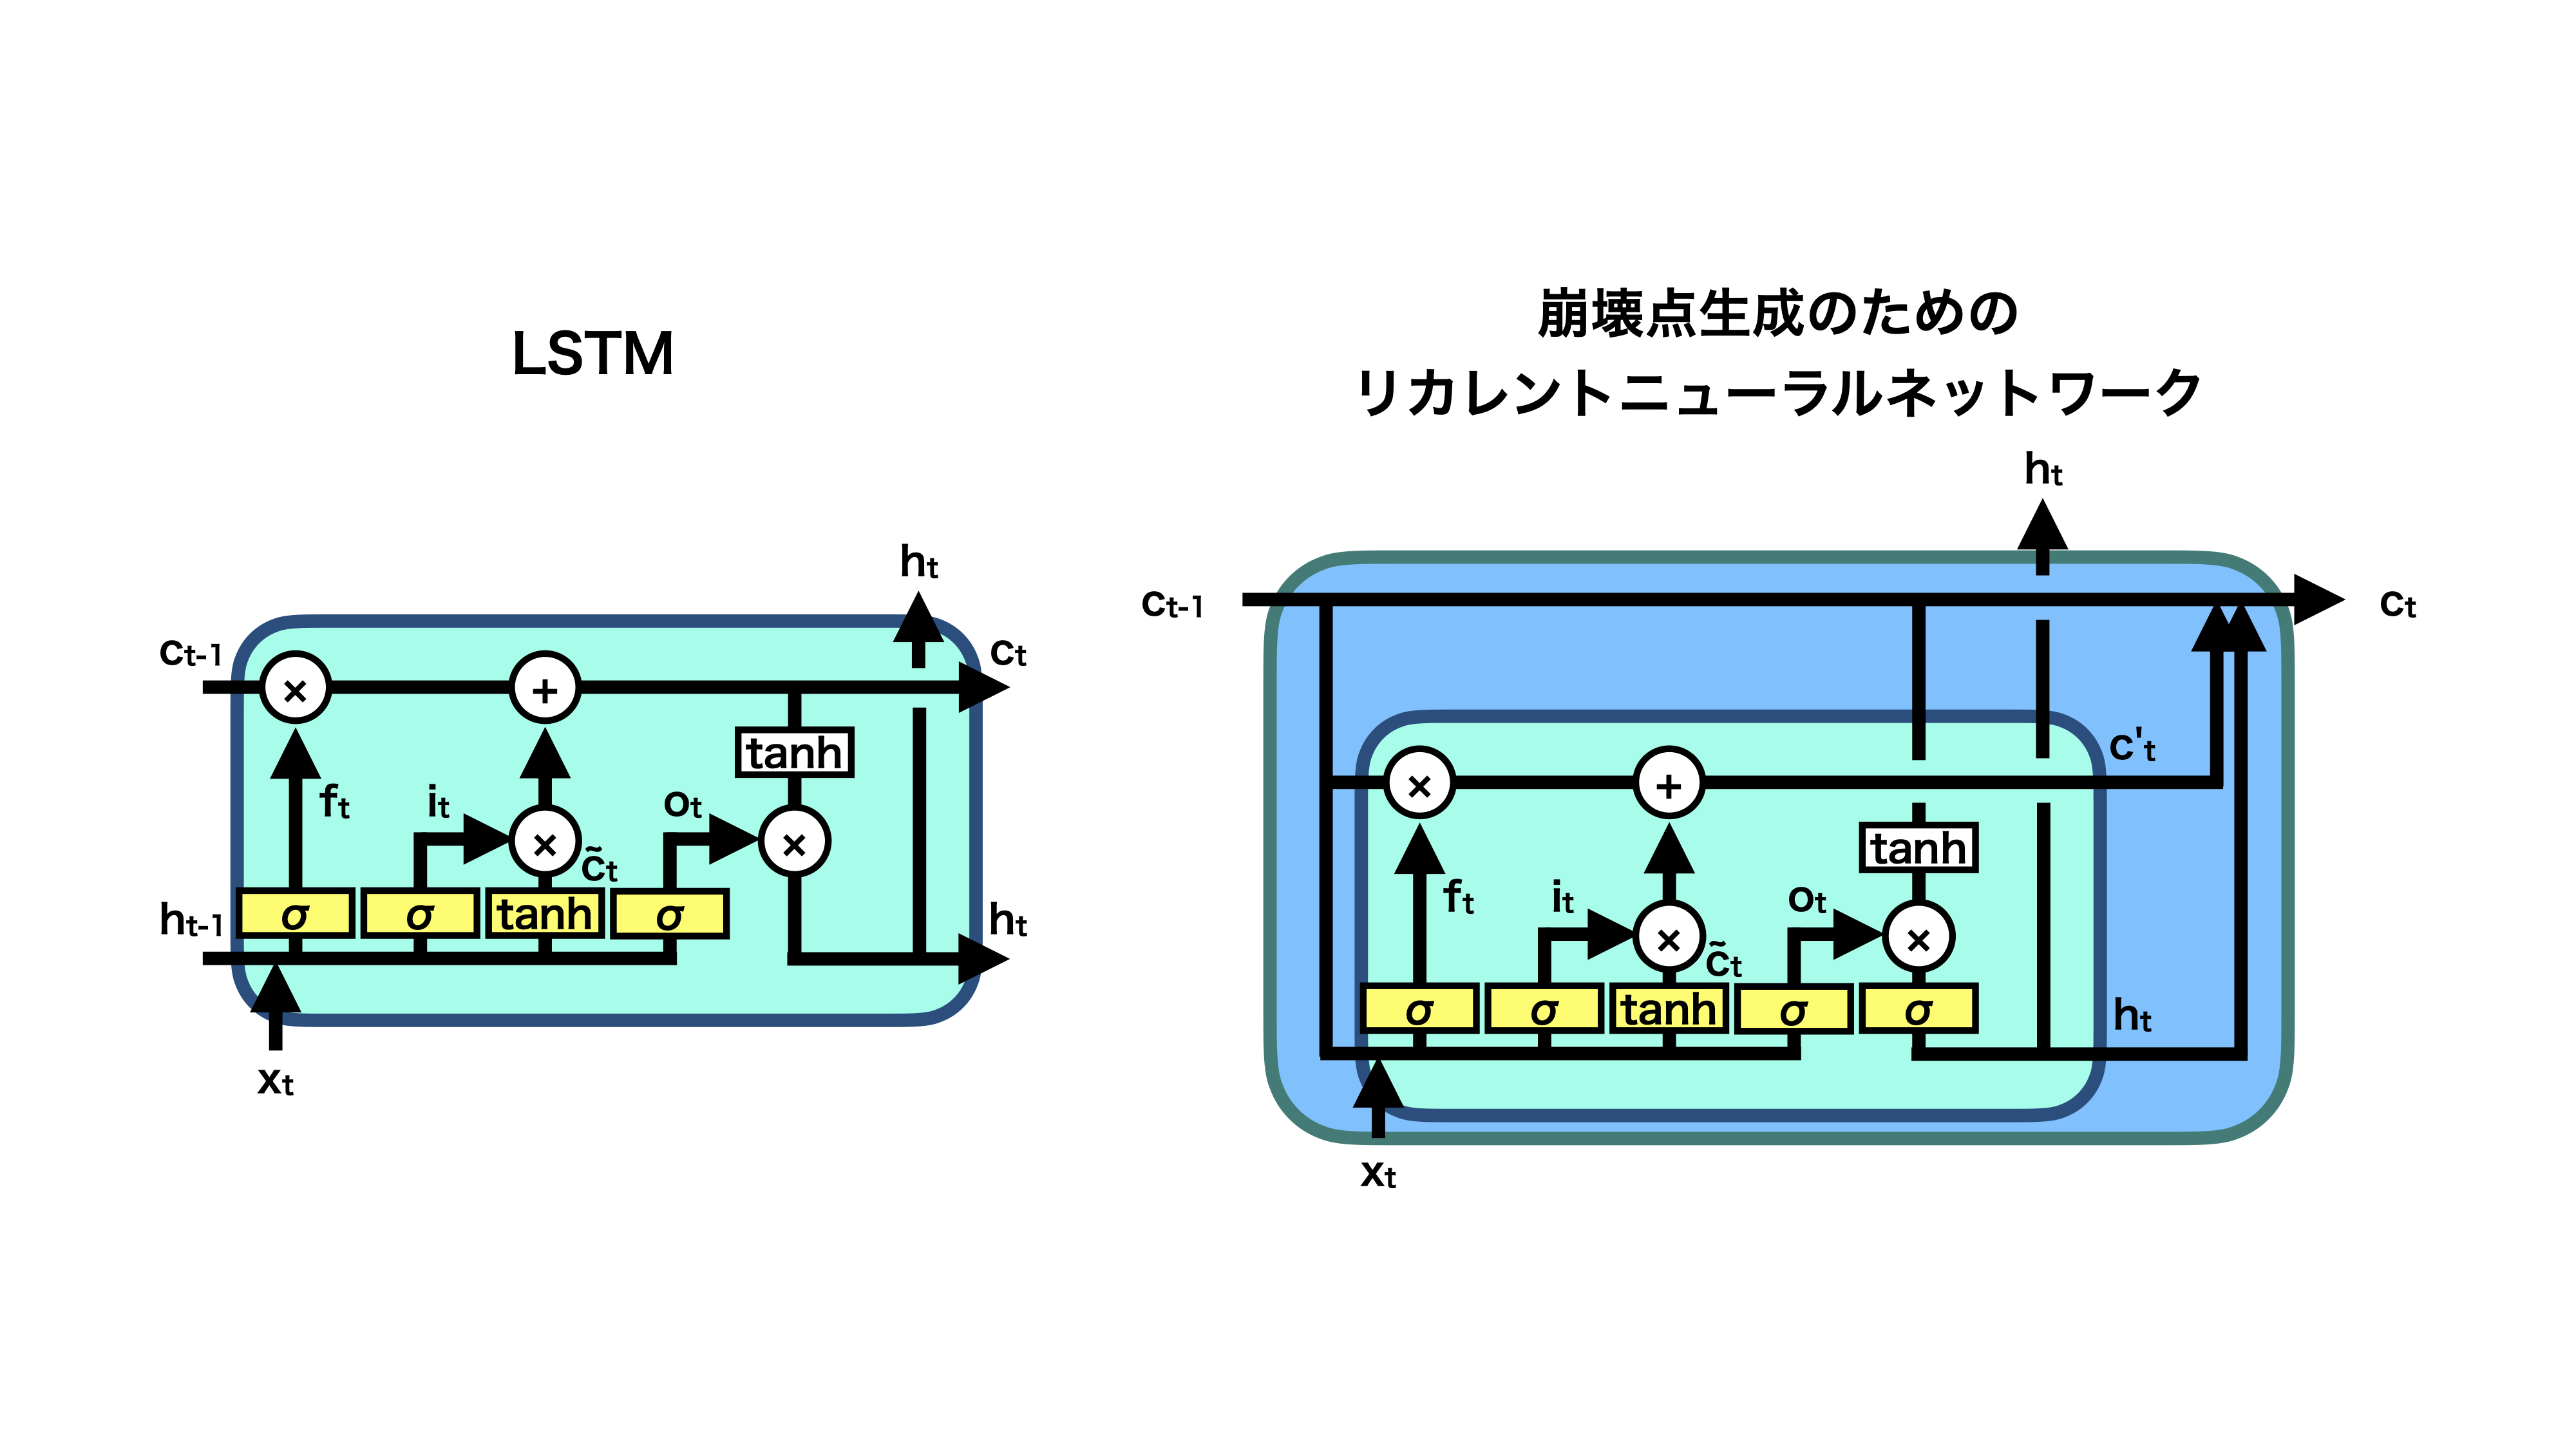
\includegraphics[trim = 0 100 0 200, width=0.9\textwidth, clip]{Figure/3Networks/3-4-1-2VLSTMStructure.png}
 \caption[系列1ステップについての独自リカレントニューラルネットワーク構造]{系列1ステップについての独自リカレントニューラルネットワーク構造。図\ref{3-4-1-1SimpleVLSTM}の青丸の一つに相当している。}
 \label{3-4-1-2VLSTMStructure}
\end{figure}

LSTMとの大きな構造の違いは、短期記憶である${\mbox{\boldmath{$h$}}}_t$が隠れ状態として入出力されていない点である。
入力は隠れ状態の記憶セル${\mbox{\boldmath{$c$}}}_{t-1}$と系列データ${\mbox{\boldmath{$x$}}}_t$の二つである。
また出力は結合・非結合を判定する${\mbox{\boldmath{$h$}}}_t$と隠れ状態の記憶セル${\mbox{\boldmath{$c$}}}_{t}$の二つである。
隠れ状態として${\mbox{\boldmath{$h$}}}_t$が使用されていないため、内部の構造も通常のLSTMとは少し異なり、出力${\mbox{\boldmath{$h$}}}_{t}$と記憶セル${\mbox{\boldmath{$c$}}}_{t}$はそれぞれ
\begin{equation}
 \begin{split}
  &{\mbox{\boldmath{$c$}}}_{t} 
  = (1-{\mbox{\boldmath{$h$}}}_t) {\mbox{\boldmath{$c$}}}_{t-1} + {\mbox{\boldmath{$h$}}}_t {\mbox{\boldmath{$c'$}}}_{t}\\
  &{\mbox{\boldmath{$c'$}}}_{t}
  = {\mbox{\boldmath{$c$}}}_{t-1} \  \sigma (W_f {\mbox{\boldmath{$x$}}}_t + R_f {\mbox{\boldmath{$c$}}}_{t-1}) 
  + \tanh (W_c {\mbox{\boldmath{$x$}}}_t + R_c {\mbox{\boldmath{$c$}}}_{t-1}) \  \sigma (W_i {\mbox{\boldmath{$x$}}}_t + R_i {\mbox{\boldmath{$c$}}}_{t-1})\\
  &{\mbox{\boldmath{$h$}}}_{t} 
  = \sigma (D_h [\tanh({\mbox{\boldmath{$c$}}}_{t-1}) \  \sigma (W_o {\mbox{\boldmath{$x$}}}_t + R_o {\mbox{\boldmath{$c$}}}_{t-1}) ])
 \end{split}
\end{equation}
となる。
第二式の${\mbox{\boldmath{$c'$}}}_{t}$は更新された記憶セルを示している。
第三式は出力ゲートに更に全結合層を掛けた形となっており、二値分類の為の出力を作成している。
第一式では、更新された記憶セル${\mbox{\boldmath{$c'$}}}_{t}$と直前の系列での記憶セル${\mbox{\boldmath{$c$}}}_{t-1}$、出力${\mbox{\boldmath{$h$}}}_{t}$を用いて現在の記憶セル${\mbox{\boldmath{$c$}}}_{t}$を計算している。
二値分類であるので、${\mbox{\boldmath{$h$}}}_{t}$は$0$から$1$の値を持つはずである。
したがって、第一式は結合(${\mbox{\boldmath{$h$}}}_{t} \sim 1$)していれば更新された記憶セル${\mbox{\boldmath{$c'$}}}_{t}$が、非結合(${\mbox{\boldmath{$h$}}}_{t} \sim 0$)であれば、直前の系列での記憶セル${\mbox{\boldmath{$c$}}}_{t-1}$が現在の記憶セル${\mbox{\boldmath{$c$}}}_{t}$となることを示している。

初期状態は崩壊点のタネであるので、以上の演算は次のように (図\ref{3-4-1-3Interpretation}) 解釈できる。

\begin{enumerate}
 \item $t-1$番目の崩壊点${\mbox{\boldmath{$c$}}}_{t-1}$と$t$番目の飛跡${\mbox{\boldmath{$x$}}}_{t}$が結合しているか否かの評価${\mbox{\boldmath{$h$}}}_{t}$を行う
 \item $t-1$番目の崩壊点${\mbox{\boldmath{$c$}}}_{t-1}$と$t$番目の飛跡${\mbox{\boldmath{$x$}}}_{t}$を用いて更新された崩壊点${\mbox{\boldmath{$c'$}}}_{t}$を計算する
 \item $t-1$番目の崩壊点${\mbox{\boldmath{$c$}}}_{t-1}$と$t$番目の飛跡${\mbox{\boldmath{$x$}}}_{t}$が結合しているならば更新された崩壊点${\mbox{\boldmath{$c'$}}}_{t}$を、結合していないならば$t-1$番目の崩壊点${\mbox{\boldmath{$c$}}}_{t-1}$を$t$番目の崩壊点${\mbox{\boldmath{$c$}}}_{t}$として選択する
\end{enumerate}

\begin{figure}[htbp]
 \centering
 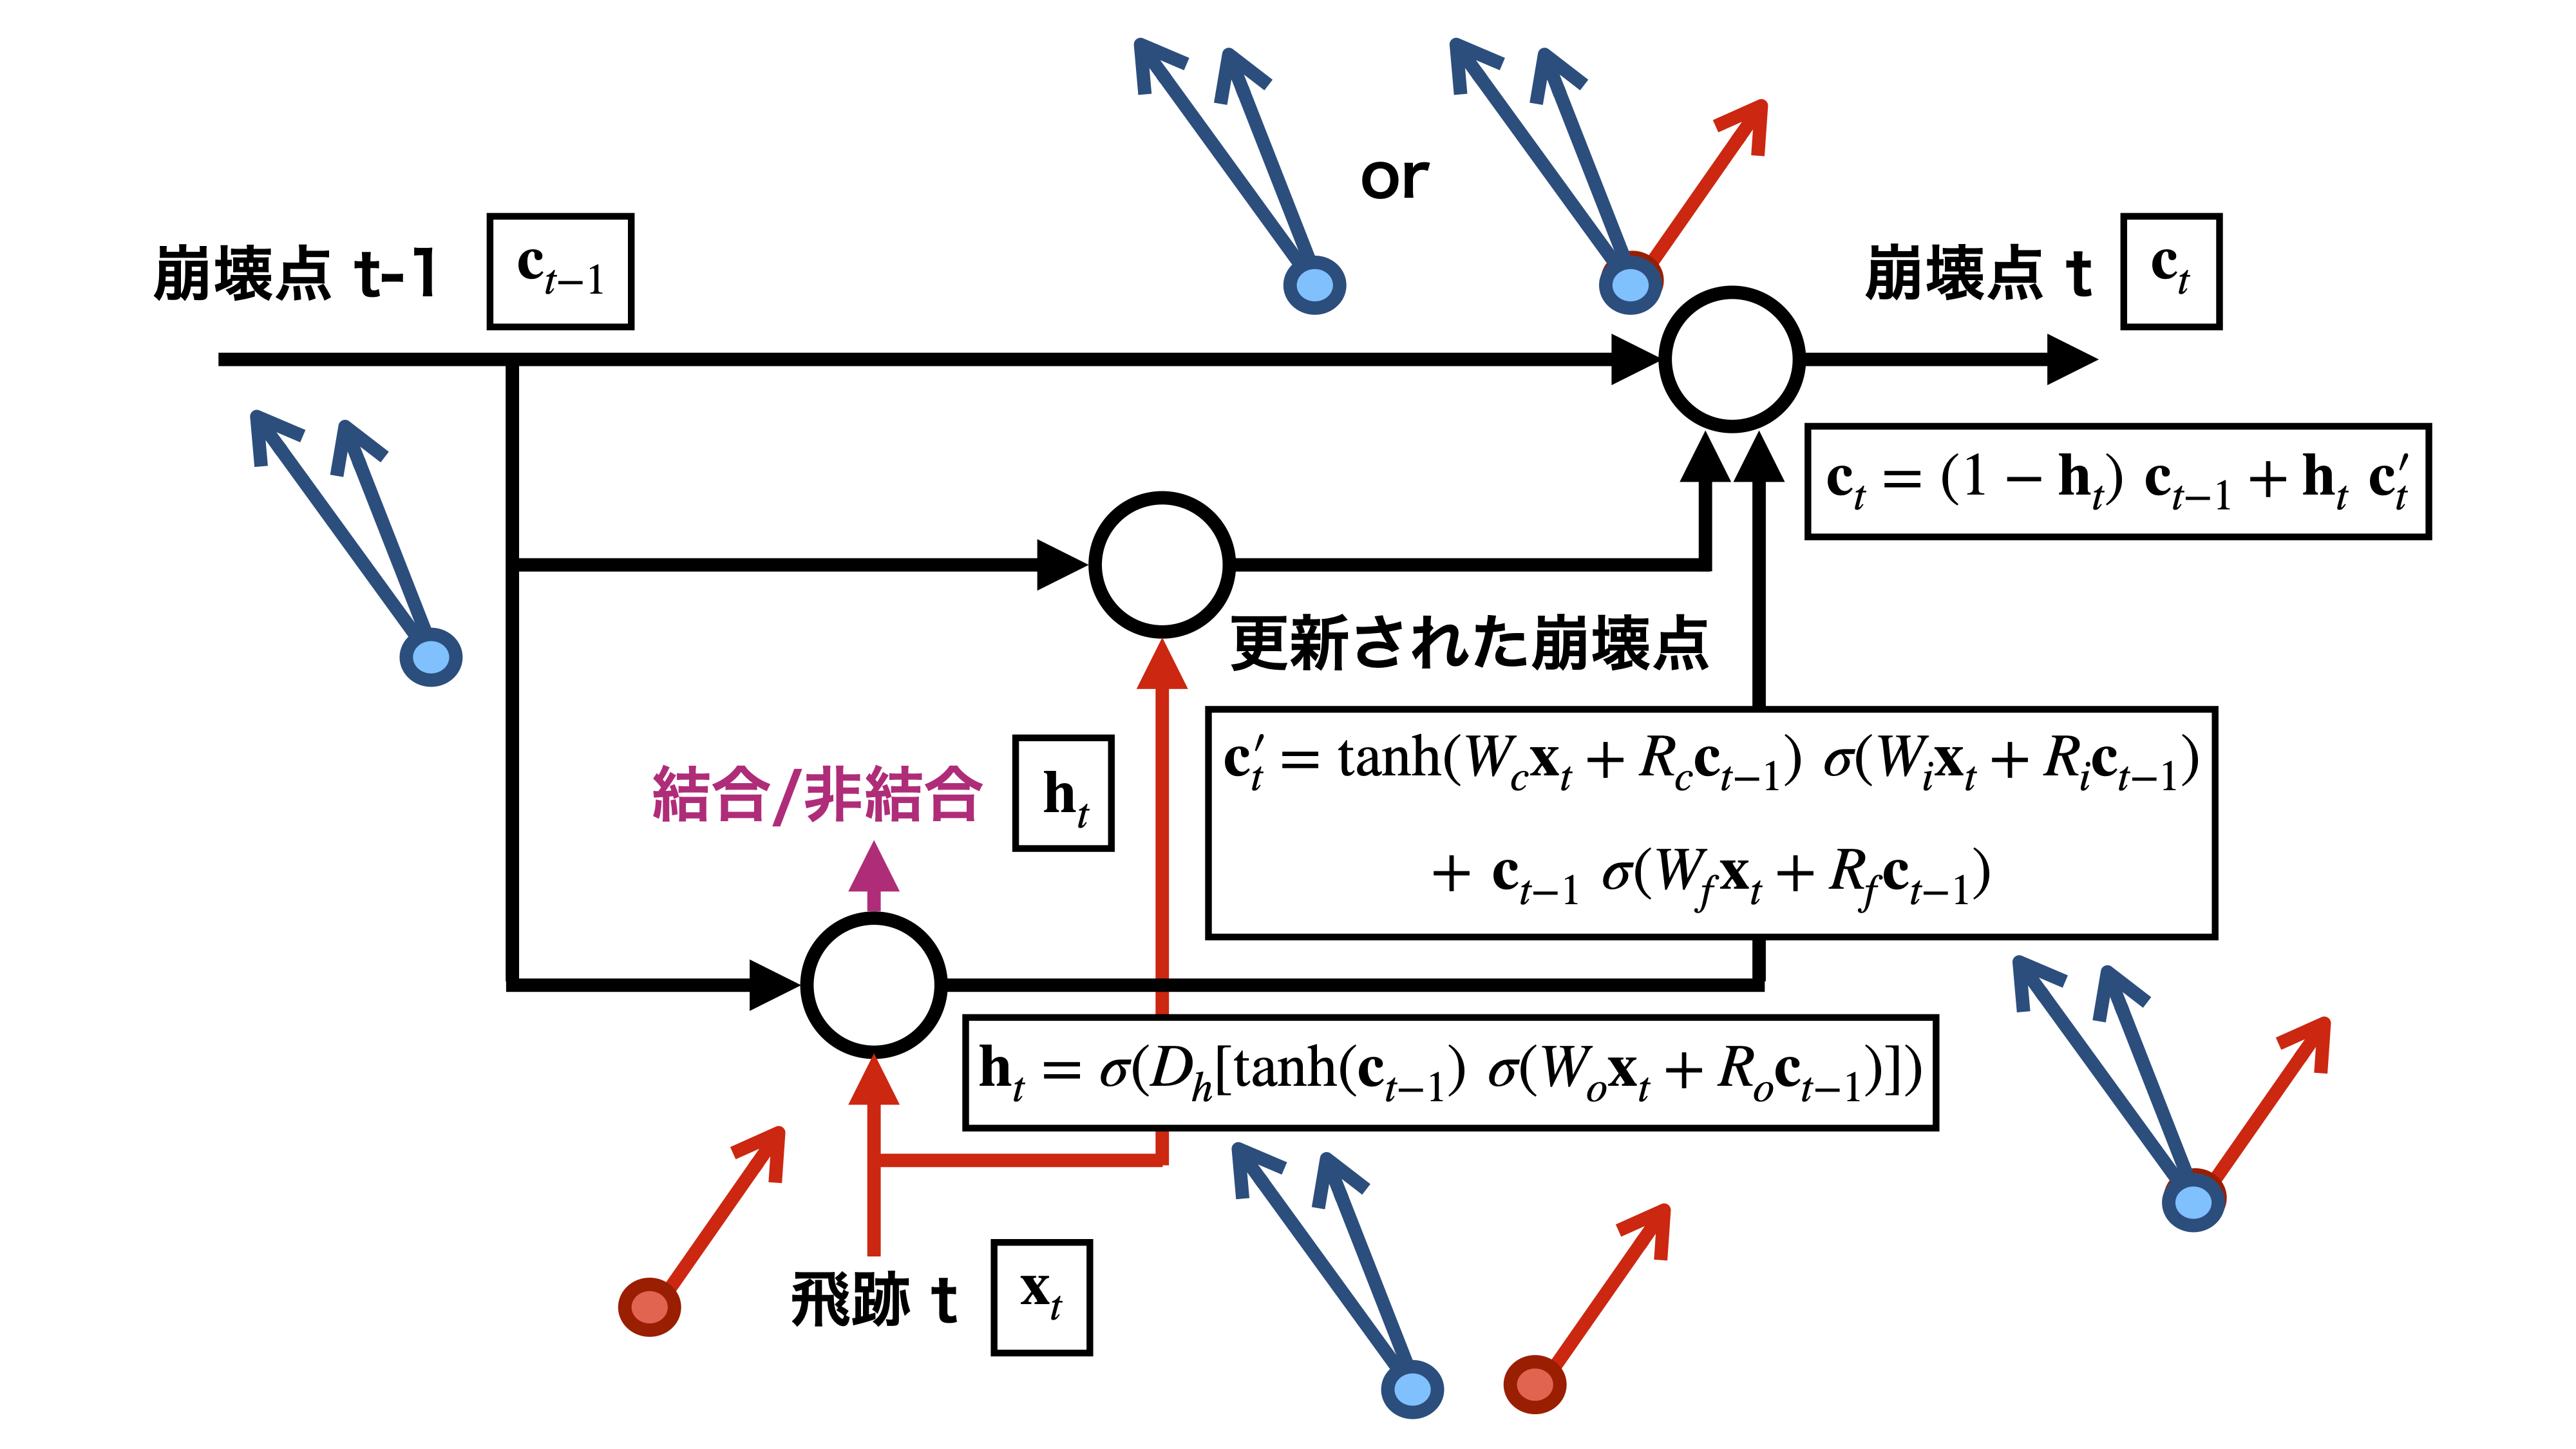
\includegraphics[width=0.9\textwidth, clip]{Figure/3Networks/3-4-1-3Interpretation.png}
 \caption[独自リカレントニューラルネットワーク構造の解釈]{独自リカレントニューラルネットワーク構造の解釈。それぞれの丸が演算に対応している。左下が演算1、中央が演算2、右上が演算3である。}
 \label{3-4-1-3Interpretation}
\end{figure}

短期記憶を破棄する事によって、独自リカレントニューラルネットワークでは、事象中の飛跡の順序 (短期記憶) にできる限り依存させず、更に崩壊点のタネに対して飛跡を足していくことによって更新される崩壊点の情報 (記憶セル) を表現している。\\

私たちはシミュレーションデータとして既に一つの事象分の全ての飛跡についての情報を持っている。
したがって、作成したリカレントニューラルネットワークをエンコーダー・デコーダーモデルに組み込むことで、事象についての情報 (コンテキスト) を活用することができると考えられる。
また、エンコーダー・デコーダーモデルの間にAttentionを組み込むことも同様に自然な発想である。
その様なネットワークを図\ref{3-4-1-4EncoderDecoderVLSTM}に示す。

\begin{figure}[htbp]
 \centering
 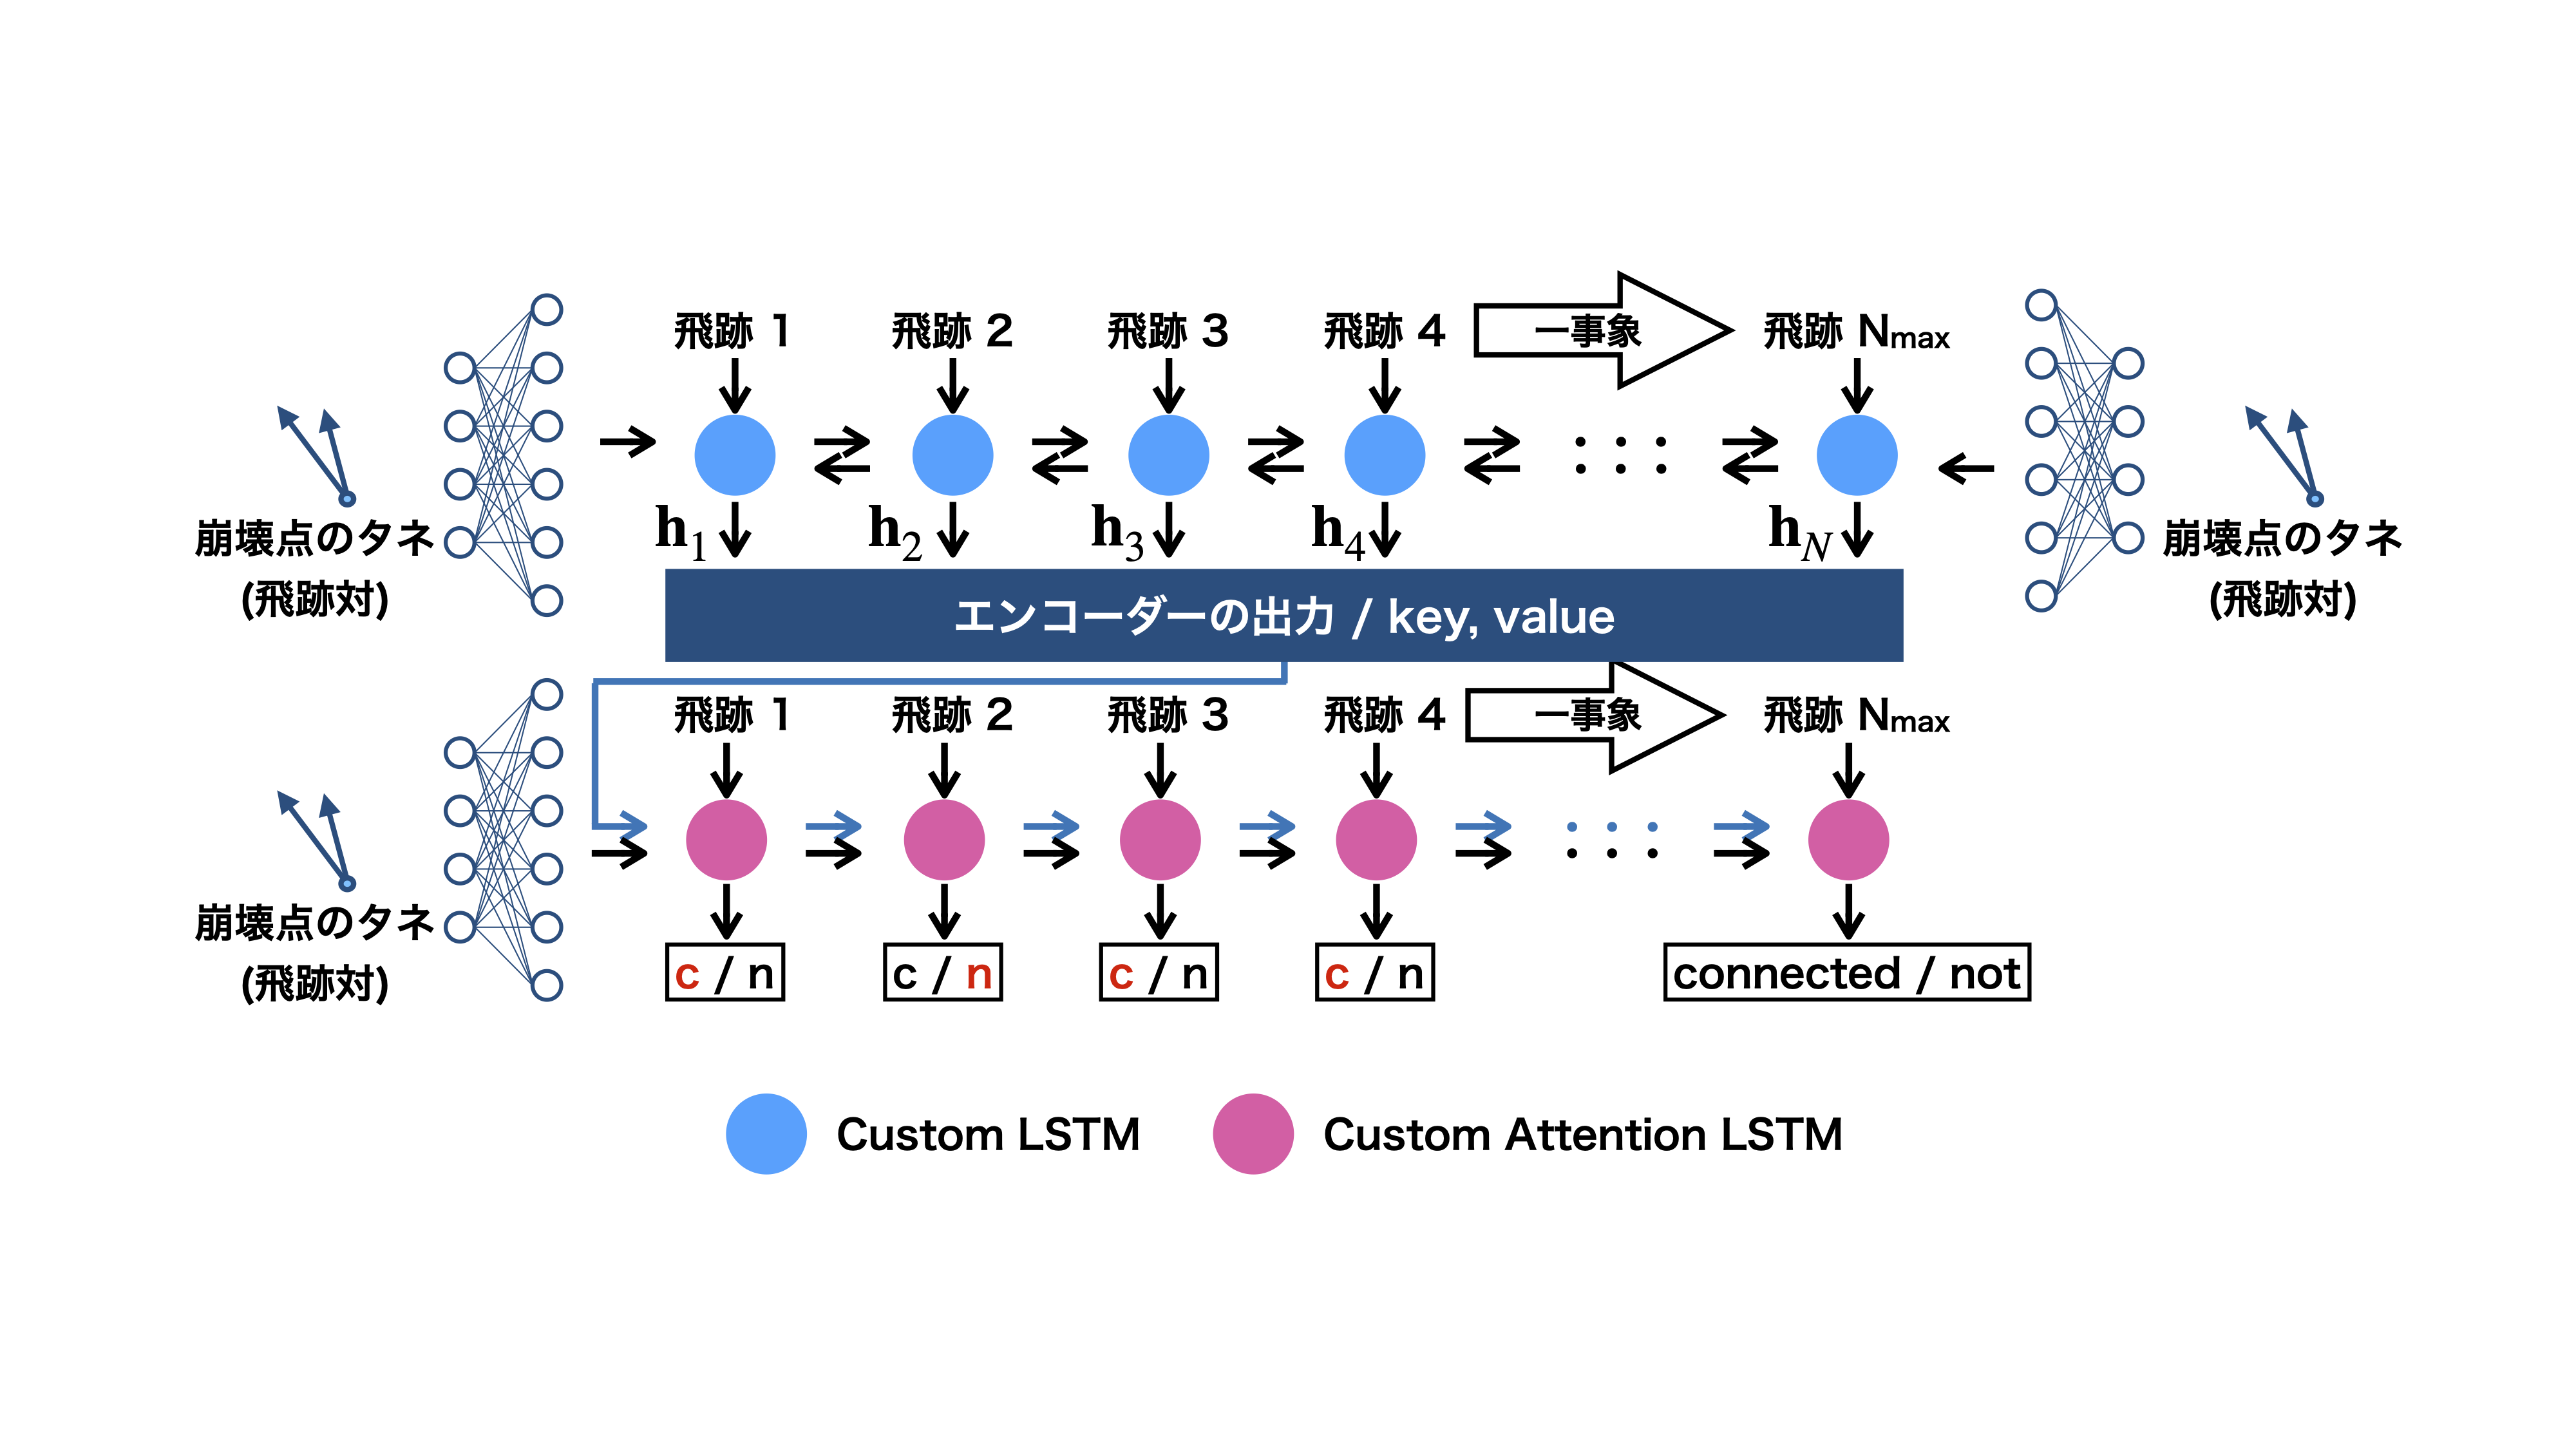
\includegraphics[trim = 100 200 100 100, width=1.0\textwidth, clip]{Figure/3Networks/3-4-1-4EncoderDecoderVLSTM.png}
 \caption[Attentionを組み込んだエンコーダー・デコーダーモデルへの拡張]{Attentionを組み込んだエンコーダー・デコーダーモデルへの拡張。図上部がエンコーダー部、図下部がデコーダー部をそれぞれ示している。初期状態や系列データはエンコーダー部とデコーダー部のそれぞれに入力されている。エンコーダー部では双方向RNNを用いている。ただし、ここのステップは独自構造のネットワークになっている。エンコーダー部の出力は図中央のKey・Valueに集められ、デコーダー部に入力される。デコーダー部での出力はそれぞれの飛跡がタネと結合しているか、非結合であるかの二値分類である。}
 \label{3-4-1-4EncoderDecoderVLSTM}
\end{figure}

図の上部はエンコーダー部である。
エンコーダー部では事象中の飛跡から事象全体の情報 (コンテキスト) を抽出している。
ここでは先ほどの図\ref{3-4-1-1SimpleVLSTM}で紹介したネットワークを双方向リカレントニューラルネットワークとして使用している。
ただし、出力${\mbox{\boldmath{$h$}}}_{t}$の次元数を減らさないようにするため全結合層$D_h$を取り除いている。
また図中で表現しているように、双方向から入力されている崩壊点のタネはそれぞれ別の全結合層によって情報を抽象化されている。

図の下部はデコーダー部である。
デコーダー部ではエンコーダー部で抽出された情報と崩壊点のタネ、事象中の飛跡を使用して崩壊点のタネにそれぞれの飛跡が結合しているか否かを判別している。
エンコーダー部で抽出された情報はAttentionによって適切に評価され、デコーダー部の"ある"飛跡がエンコーダー部の任意の飛跡に対して注意を払って、事象中の情報を取得できるようになっている。
またエンコーダー・デコーダーモデルへの拡張後も、このネットワークの基本構造がリカレントニューラルネットワークであることに変わりはない為、飛跡の本数を任意に変えることが可能である。

図\ref{3-4-1-2VLSTMStructure}で示したネットワーク構造はAttentionには対応していないため、新たなネットワークの構築が必要である。
そのようなネットワークを図\ref{3-4-1-5AttentionVLSTM}に示す。

\begin{figure}[htbp]
 \centering
 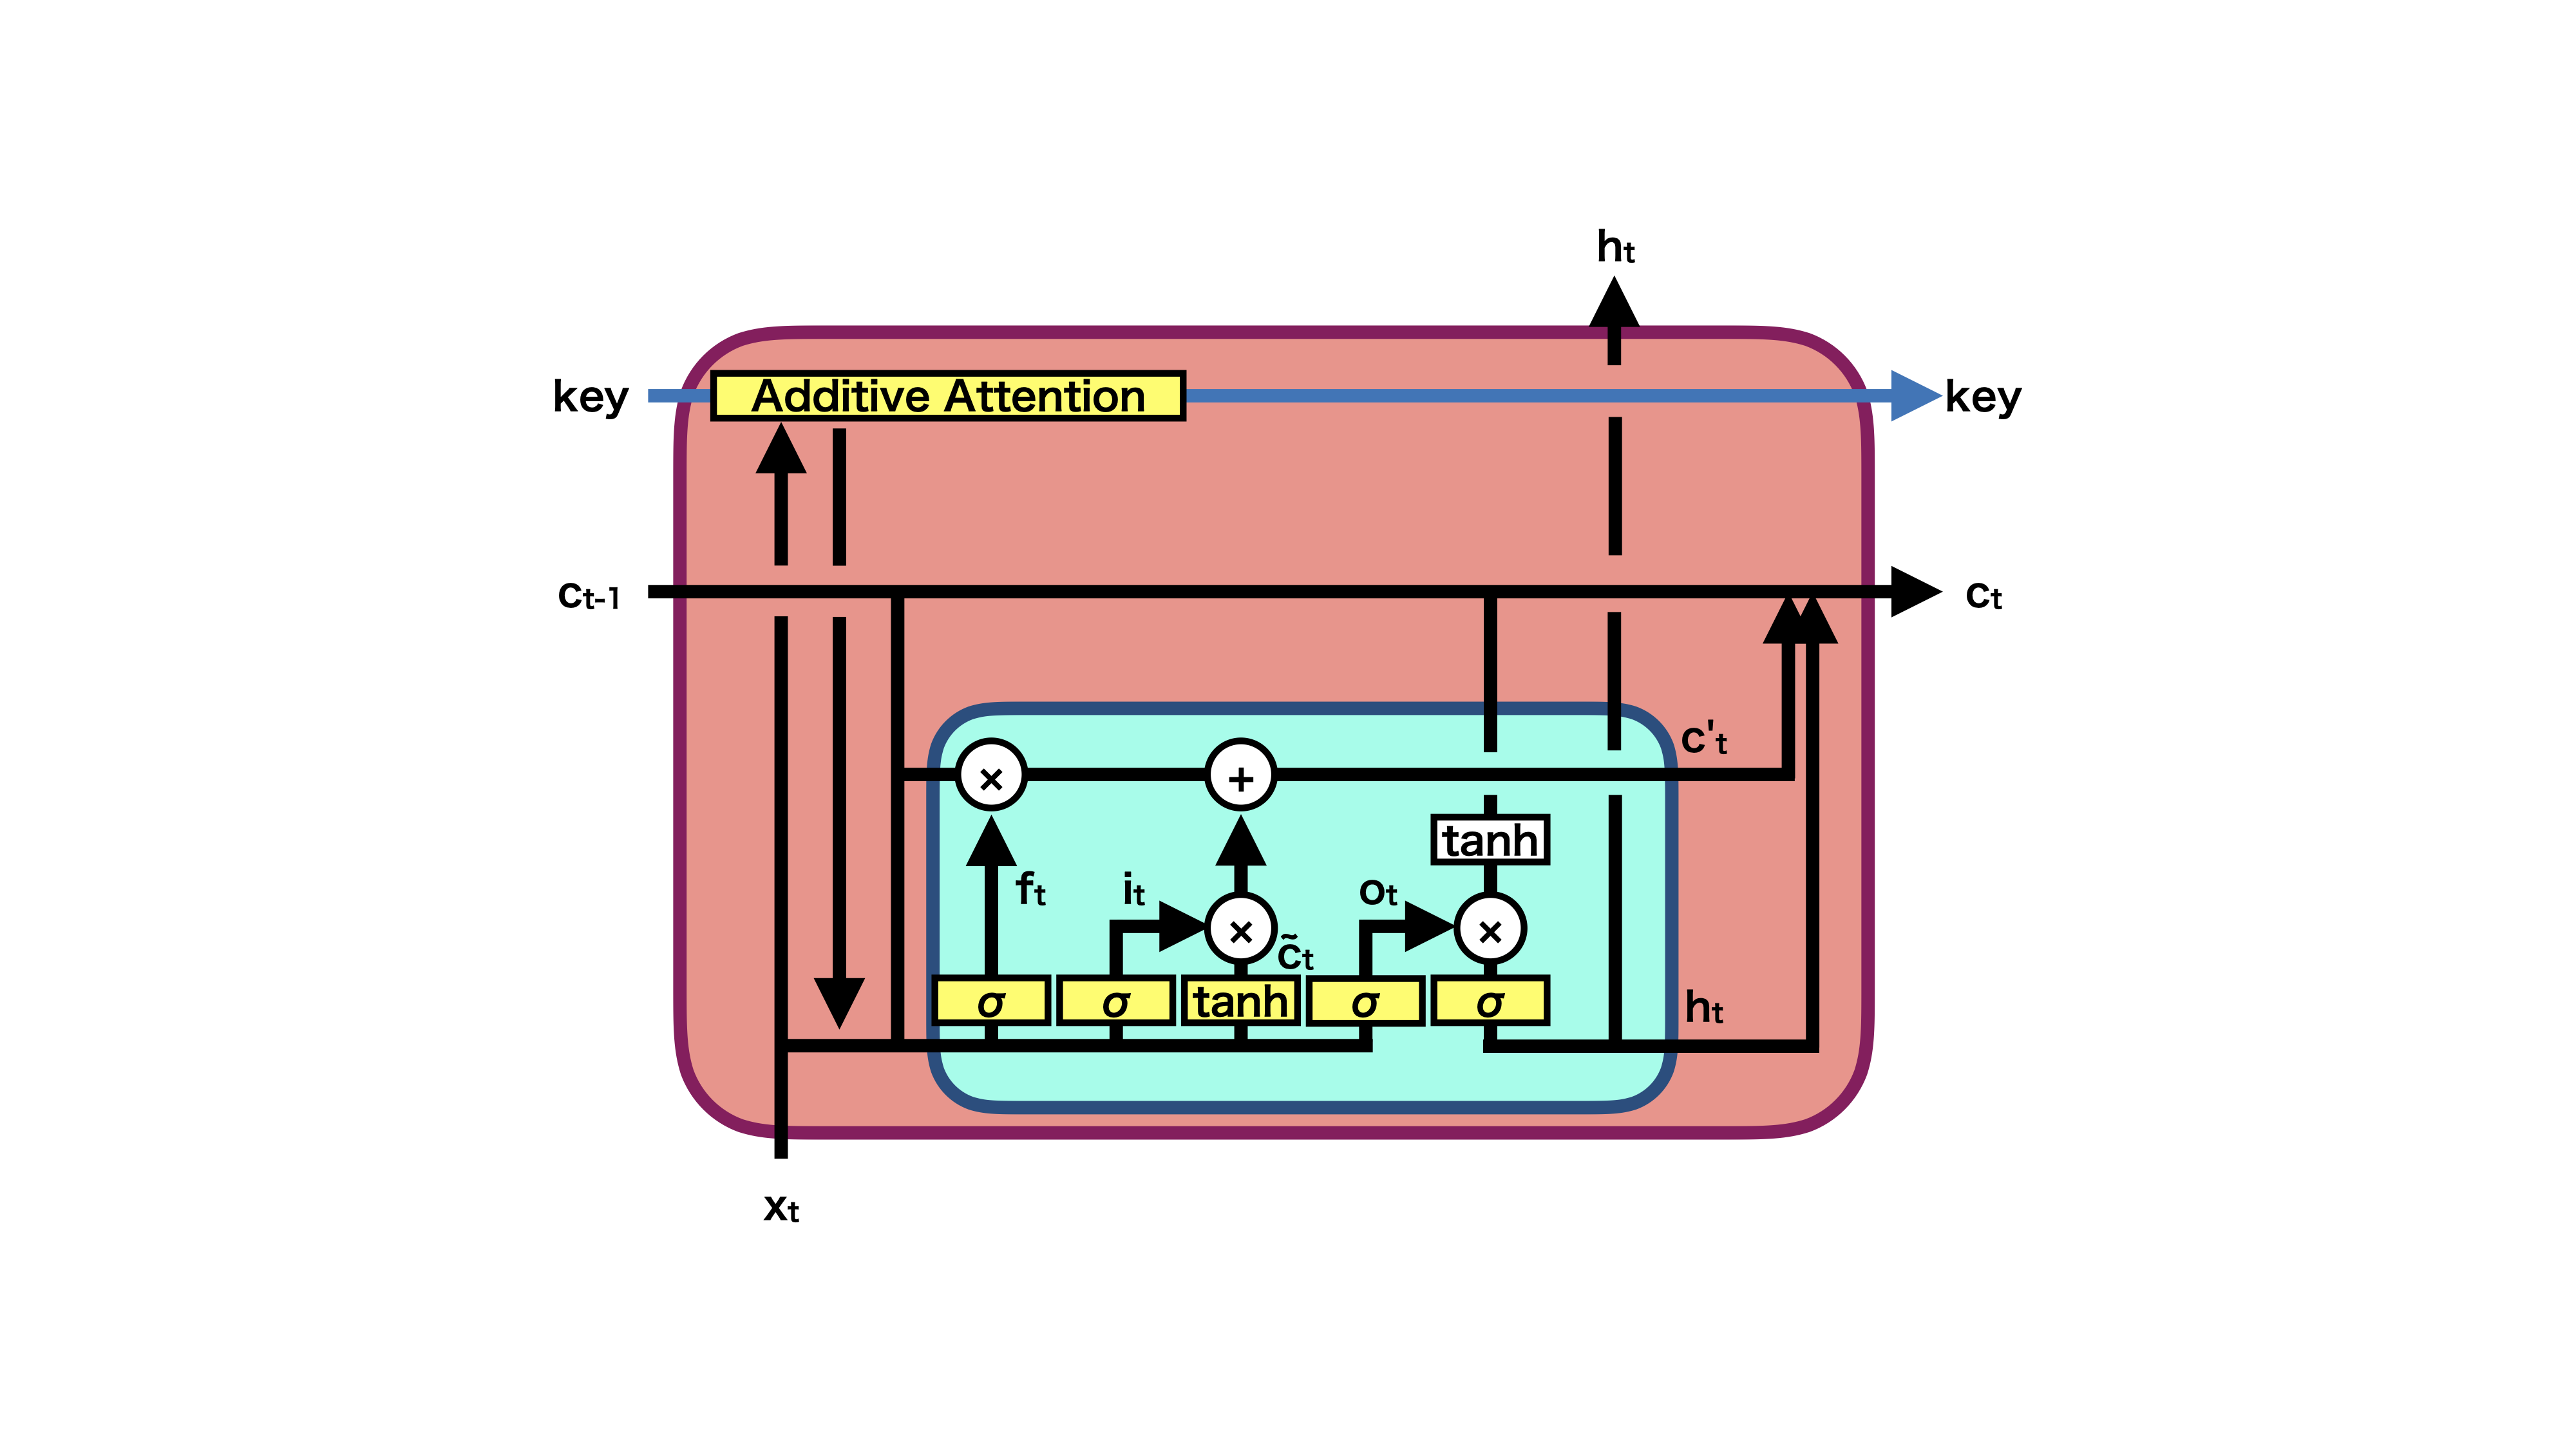
\includegraphics[trim = 100 0 100 0, width=0.9\textwidth, clip]{Figure/3Networks/3-4-1-5AttentionVLSTM.png}
 \caption[独自リカレントニューラルネットワークのAttentionへの拡張]{独自リカレントニューラルネットワークのAttentionへの拡張。図\ref{3-4-1-4EncoderDecoderVLSTM}の赤丸の一つに相当している。図上部の青線は不変記憶Key・Valueの流れを表している。Attentionに関する演算が加えられている点以外は図\ref{3-4-1-2VLSTMStructure}と同様の構造である。}
 \label{3-4-1-5AttentionVLSTM}
\end{figure}

本研究では、エンコーダー部で抽出された情報 (Key) をリカレントニューラルネットワークの隠れ状態の一つとして入力している。
また、このKeyはネットワークの各ステップについて共通の値を使用しており、長期記憶・短期記憶と比べて不変記憶のような役割を果たしている。
Attention Weightの計算方法としてAdditive Attentionを採用した。
$t$番目のコンテキスト${\mbox{\boldmath{$\gamma$}}}_{t}$は次のように計算される。
\begin{equation}
 \begin{split}
  {\mbox{\boldmath{$\gamma$}}}_{t} 
  &= {\mbox{\boldmath{$\alpha$}}}_{t} V\\
  {\mbox{\boldmath{$\alpha$}}}_{t}
  &= (\alpha_{t,0},\ \alpha_{t,1},\ \alpha_{t,2},\ \cdots \alpha_{t,i},\ \cdots) \\
  &= \left(\frac{\exp{({{e}}_{t,0})}}{\sum_j \exp{({{e}}_{t,j})}},\ \frac{\exp{({{e}}_{t,1})}}{\sum_j \exp{({{e}}_{t,j})}},\ \frac{\exp{({{e}}_{t,2})}}{\sum_j \exp{({{e}}_{t,j})}},\  \cdots \frac{\exp{({{e}}_{t,i})}}{\sum_j \exp{({{e}}_{t,j})}},\ \cdots\right)\\
  {\mbox{\boldmath{$e$}}}_{t}
  &={\mbox{\boldmath{$u$}}}_{\rm energy} (K\ U_{\rm key} + X_t\ U_{\rm query}) \\
 \end{split}
\end{equation}
ここで、Keyを$K$、Valueを$V$、$t$番目のQueryである飛跡${\mbox{\boldmath{$x$}}}_{t}$を重ねた行列を$X_t$、$t$番目のAttention Weightを${\mbox{\boldmath{$\alpha$}}}_{t}$、$t$番目のQueryについてのエネルギーを${\mbox{\boldmath{$e$}}}_{t}$とした。
また、Additive Attentionにおける重み行列をそれぞれ${\mbox{\boldmath{$u$}}}_{\rm energy},\  U_{\rm key},\ U_{\rm query}$と置いた。

添字$i,\ j$はエンコーダー部の系列、添字$t$はデコーダー部の系列である。
したがって$t$番目のAttention Weight${\mbox{\boldmath{$\alpha$}}}_{t}$はエンコーダー部の飛跡の数だけ要素を持っており、デコーダー部の全ての飛跡についてAttention Weightを計算した時、Attention Weightはエンコーダー部の飛跡の数$\times$デコーダー部の飛跡の数の行列となる。
このAttention Weight行列はネットワーク内部を把握する上で非常に重要な情報である。
図\ref{3-4-1-5AttentionVLSTM}では表現していないがオプションとしてAttention Weightを出力することで、ネットワーク内部をある程度理解することができる。

得られた$t$番目のコンテキスト${\mbox{\boldmath{$\gamma$}}}_{t}$は、出力${\mbox{\boldmath{$h$}}}_{t}$や更新された崩壊点${\mbox{\boldmath{$c'$}}}_{t}$の計算に使用される。
\begin{equation}
 \begin{split}
  &{\mbox{\boldmath{$c$}}}_{t} 
  = (1-{\mbox{\boldmath{$h$}}}_t) {\mbox{\boldmath{$c$}}}_{t-1} + {\mbox{\boldmath{$h$}}}_t {\mbox{\boldmath{$c'$}}}_{t}\\
  &{\mbox{\boldmath{$c'$}}}_{t}
  = {\mbox{\boldmath{$c$}}}_{t-1} \  \sigma (W_f {\mbox{\boldmath{$x$}}}_t + R_f {\mbox{\boldmath{$c$}}}_{t-1} + C_f {\mbox{\boldmath{$\gamma$}}}_{t})\\
  &+ \tanh (W_c {\mbox{\boldmath{$x$}}}_t + R_c {\mbox{\boldmath{$c$}}}_{t-1} + C_c {\mbox{\boldmath{$\gamma$}}}_{t}) \  \sigma (W_i {\mbox{\boldmath{$x$}}}_t + R_i {\mbox{\boldmath{$c$}}}_{t-1} + C_i {\mbox{\boldmath{$\gamma$}}}_{t})\\
  &{\mbox{\boldmath{$h$}}}_{t} 
  = \sigma (D_h [\tanh({\mbox{\boldmath{$c$}}}_{t-1}) \  \sigma (W_o {\mbox{\boldmath{$x$}}}_t + R_o {\mbox{\boldmath{$c$}}}_{t-1} + C_o {\mbox{\boldmath{$\gamma$}}}_{t}) ])
 \end{split}
\end{equation}
式中ではコンテキスト${\mbox{\boldmath{$\gamma$}}}_{t}$に関する各ゲートそれぞれの重み行列を$C_f,\ C_c,\ C_i,\ C_o$と置いた。
$t$番目のコンテキスト${\mbox{\boldmath{$\gamma$}}}_{t}$についての演算を加えている点以外は図\ref{3-4-1-2VLSTMStructure}でのネットワークの演算と全く同様である。


%%%%%%%%%%%%%%%%%%%%%%%%%%%%%%%%%%%%%%%%%%%%%%%%%%%%%%%%%%%%%%%%%%%%%%%%
\subsection{ネットワークの学習と戦略} \label{Net:VLSTM:TrainingandStrategyofVLSTM}

訓練データとして必要な情報は、初期状態としての飛跡対 (崩壊点のタネ) と事象中の全ての飛跡である。
また、正解ラベルはそれぞれの飛跡が崩壊点のタネと結合しているか否かのMC情報である。
推論時は、初期状態の崩壊点のタネとして非結合な飛跡対が入力される場合が考えられるが、本研究ではネットワークの学習時は崩壊点のタネとして結合している飛跡対 (PV・SVCC・SVBB・TVCC) のみを使用する。
ここで、準崩壊点SVBCは崩壊点生成において雑音となりうる可能性があるため含んでいない。

リカレントニューラルネットワークでは、推論時は系列長を変えることができるが、学習時は重み更新の計算のため系列長を揃える必要がある。\footnote{実際にはバッチサイズ毎に}
ここでの系列長は事象中の飛跡の本数であった。
このため、不足している飛跡の本数をゼロ埋め (Zero padding) し、ゼロ埋めした飛跡が学習に影響しないよう損失関数においてマスクしている。
本研究では最も飛跡数の多い事象との兼ね合いから系列長を$60$本とし、それ以下の本数の事象については$60$本となるようにゼロ埋めしている。

最終的な入力変数の大きさを表\ref{VLSTMInputParameterShape}に示す。

\begin{table}[htb]
 \centering
 \small
  \begin{tabular}{c | c c}\hline
    & PV & SV\\\hline
    崩壊点のタネ & $(1661307,\ 44)$ & $(367434,\ 44)$\\
    事象中の全ての飛跡 & $(1661307,\ 60,\ 23)$ & $(367434,\ 60,\ 23)$\\\hline
  \end{tabular}
  \caption{任意の数の飛跡についてのネットワークの入力変数の大きさ}
  \label{VLSTMInputParameterShape}
\end{table}

ここで、第一引数はデータのサンプル数である。
訓練データは全ての崩壊点のタネについて一つのサンプルが生成されるため、全ての事象 ($\rm c\bar{c}-05,\ \rm b\bar{b}-06$) を使用すると非常に時間がかかる。
よって、本研究では全ての事象を使用して訓練データを作成した後、1エポック毎にランダムに$50000$サンプルを訓練に$10000$サンプルを検証に使用している。
事象中の全ての飛跡については飛跡の本数である$60$本とそれぞれの飛跡について$22$個の変数を持っている。
また、ゼロ埋めした飛跡との区別のためのマスク変数 $(0,\ 1)$ を一つ加えている。

崩壊点生成において、飛跡は順序を持って足されていく。
短期的な順序に依存しないような独自のネットワークを構築しているが、そのような人によって決められた飛跡の順序にネットワークが依存してしまうことは、できる限り避けねばならないため、1エポック毎に飛跡の系列順をランダムにシャッフルしている。

\begin{figure}[htbp]
 \centering
 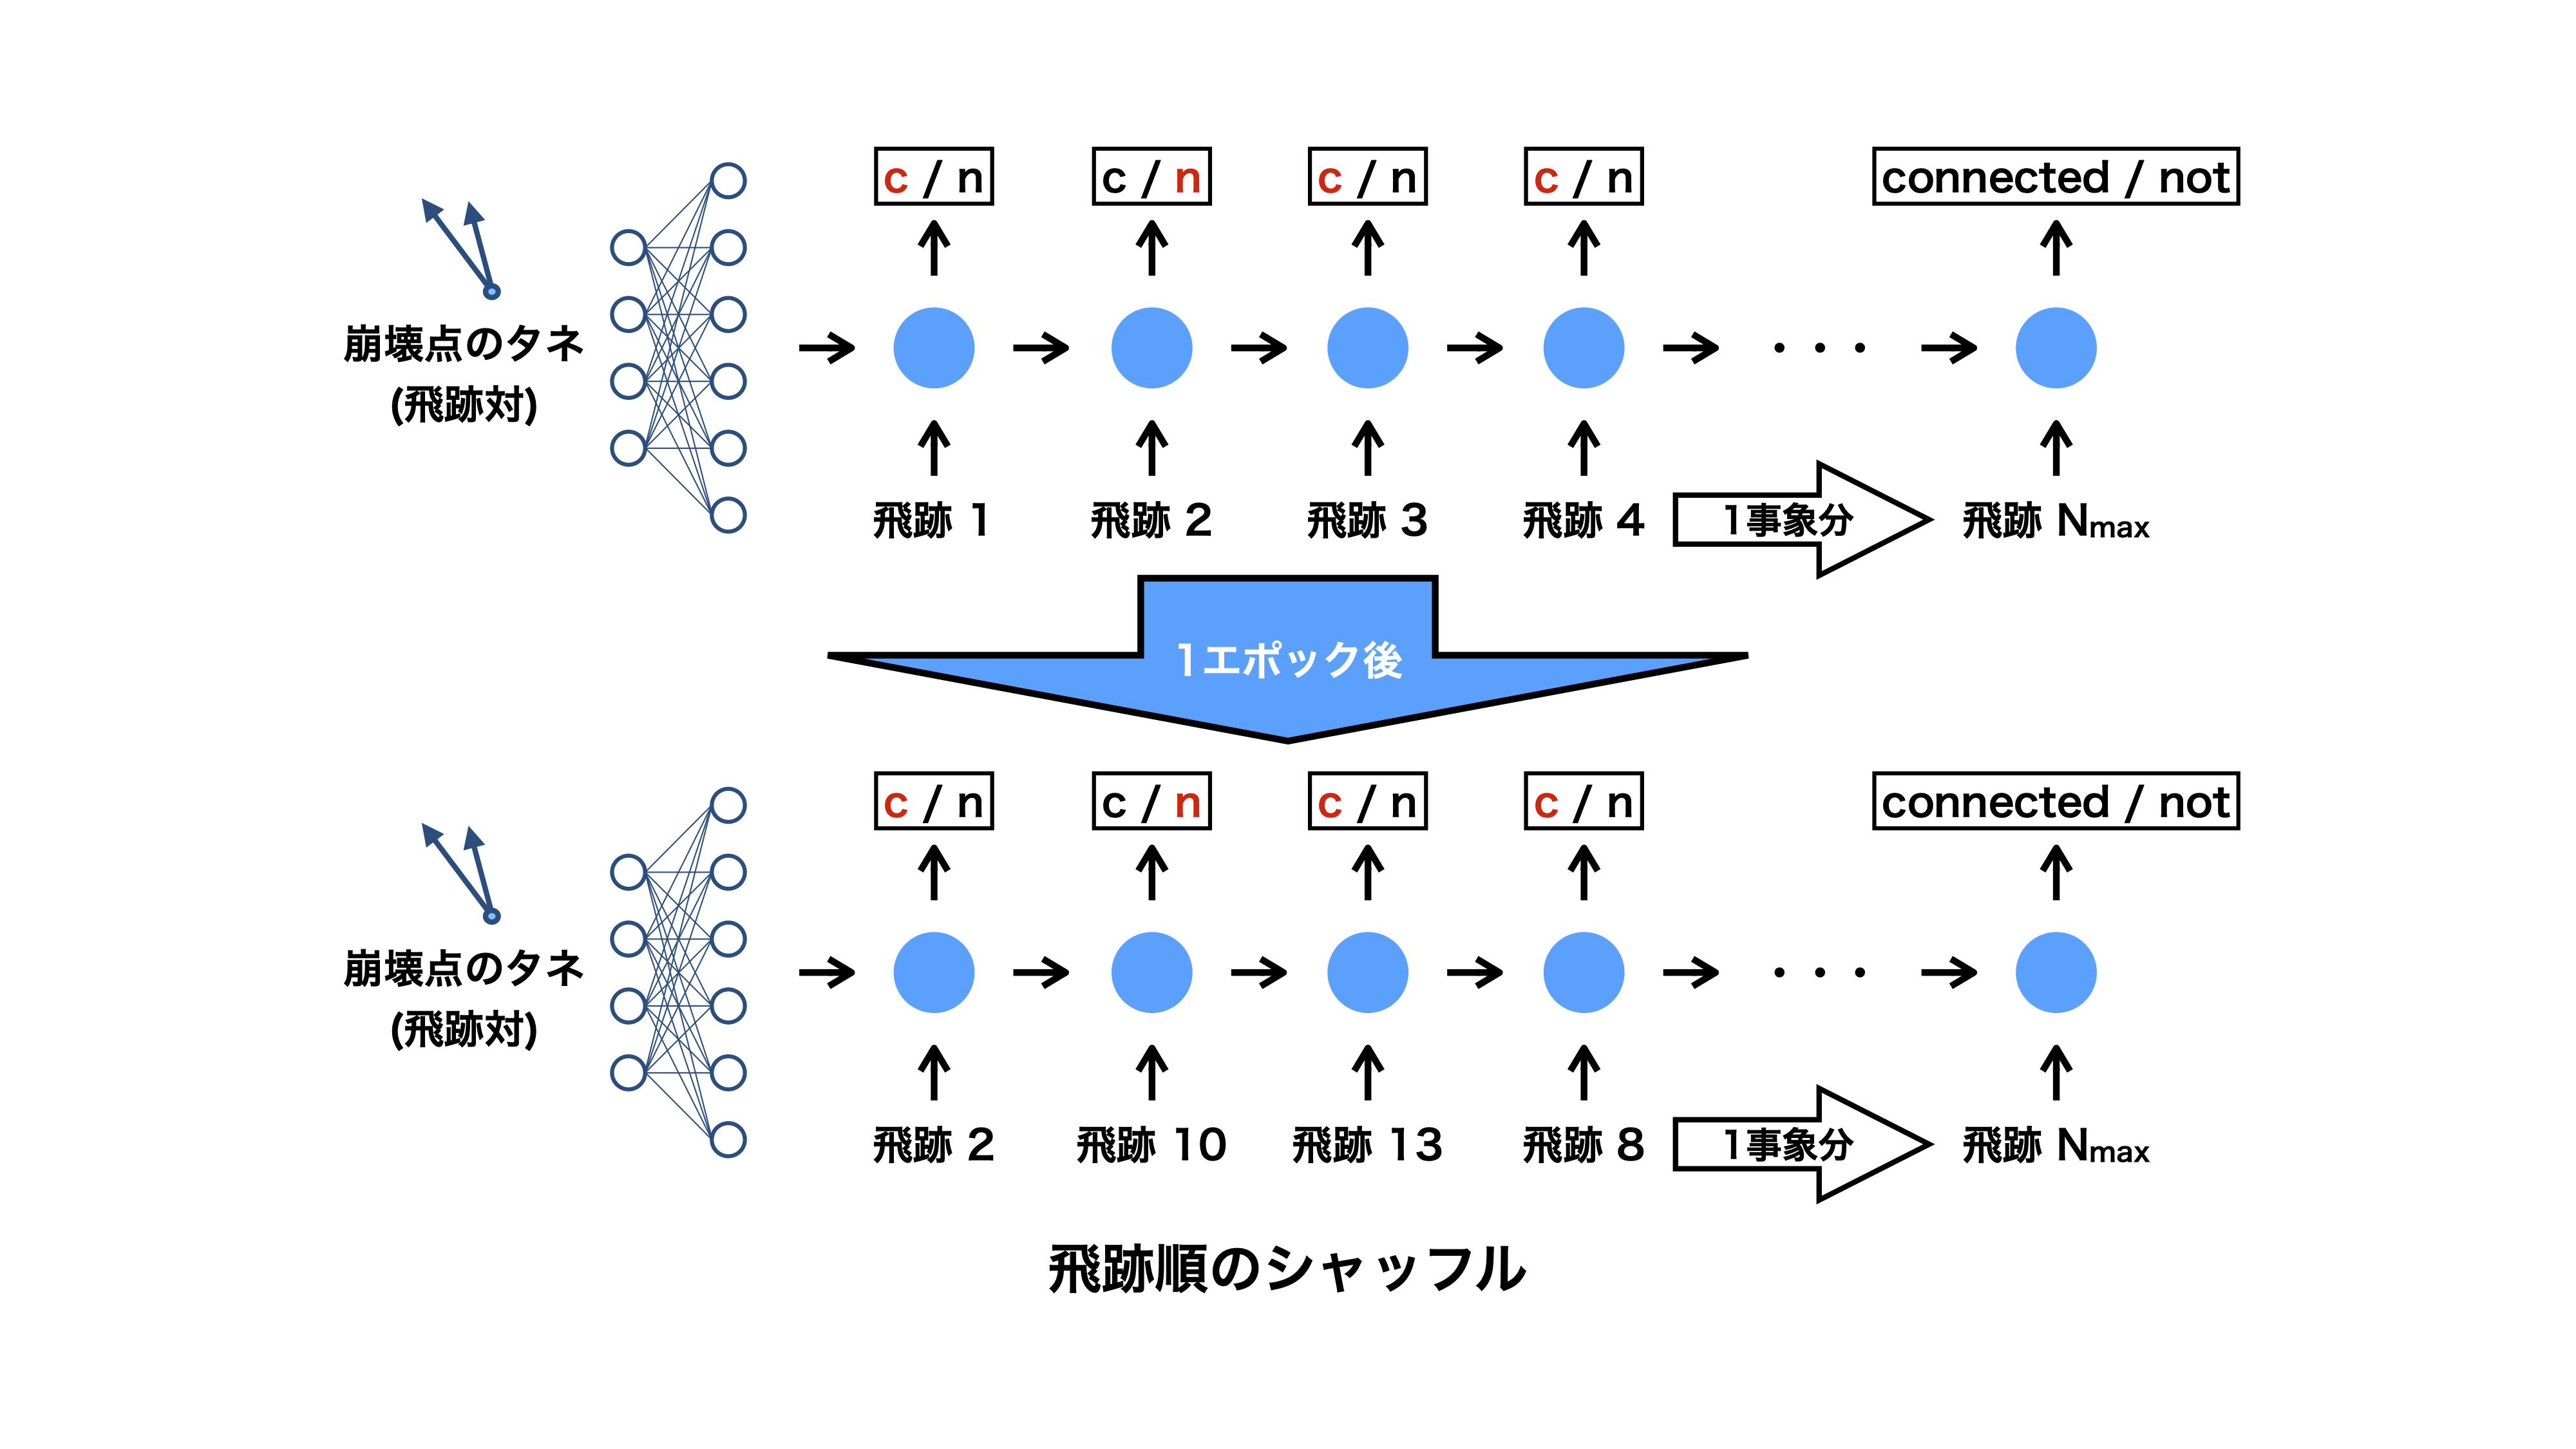
\includegraphics[trim = 150 100 150 100, width=0.9\textwidth, clip]{Figure/3Networks/3-4-2-1TrackShuffle.png}
 \caption[飛跡順のシャッフル]{飛跡順のシャッフル。$1$エポック毎に系列データの飛跡順序をシャッフルし、崩壊点のタネへ足し合わせる順番への依存を取り除いた。この順序のシャッフルは学習や検証に使用する全てのデータについて同一である。}
 \label{3-4-2-1TrackShuffle}
\end{figure}

損失関数は二値交差エントロピー誤差を使用した。
ただし、前述したようにゼロ埋めした飛跡については損失関数や正答率の計算ではマスクした。
\begin{equation}
 \begin{split}
 L = -M_{\rm ZP}\ t_{\rm C} \log{(y_{\rm C})} - M_{\rm ZP}\ (1-t_{\rm C})\ \log{(1-y_{\rm C})}
 \end{split}
\end{equation}
$M_{\rm ZP}$はゼロ埋めのためのマスク変数 $(0,\ 1)$ である。

ハイパーパラメータとして、最適化手法はAdam、学習率は$0.001$、エポック数は$100$、バッチサイズは$32$を用いた。
また、ネットワークの学習可能な重みのパラメータ数を表\ref{ParametersforVLSTMModel}に示す。

\begin{table}[htb]
 \centering
 \small
 \scalebox{0.8}{
  \begin{tabular}{l c c c}\hline
    層の名称 & 出力の形状 & パラメータ数 & 接続先\\\hline\hline
    Pair Input & (None, 44) & 0 & \\\hline
    Encoder Input & (None, 60, 23) & 0 \\\hline
    Decoder Input & (None, None, 23) & 0 \\\hline\hline
    Encoder Forward Dense 1 & (None, 256) & 11520 & Pair Input[0][0]\\\hline
    Encoder Backward Dense 1 & (None, 256) & 11520 & Pair Input[0][0]\\\hline
    Encoder Forward Activation 1 & (None, 256) & 0 & Encoder Forward Dense 1[0][0]\\\hline
    Encoder Backward Activation 1 & (None, 256) & 0 & Encoder Backward Dense 1[0][0]\\\hline
    Encoder Forward Dense 2 & (None, 256) & 11520 & Encoder Forward Activation 1[0][0]\\\hline
    Encoder Backward Dense 2 & (None, 256) & 11520 & Encoder Backward Activation 1[0][0]\\\hline
    Encoder Forward Activation 2 & (None, 256) & 0 & Encoder Forward Dense 2[0][0]\\\hline
    Encoder Backward Activation 2 & (None, 256) & 0 & Encoder Backward Dense 2[0][0]\\\hline\hline
    Encoder Embedding Dense & (None, 60, 256) & 6144 & Encoder Input[0][0]\\\hline\hline
    Bidirectional Encoder VLSTM & (None, 60, 512) & 1050624 & Encoder Embedding Dense[0][0]\\     
                                                                                                         &&&Encoder Forward Activation 2[0][0]\\       
                                                                                                         &&&Encoder Forward Activation 2[0][0]\\       
                                                                                                         &&&Encoder Backward Activation 2[0][0]\\     
                                                                                                         &&&Encoder Backward Activation 2[0][0]\\ \hline
    Reshape Bidirectional Encoder & (None, 27136) & 0 & Bidirectional Encoder VLSTM[0][0]\\\hline\hline
    Decoder Dense 1 & (None, 256) & 11520 & Pair Input[0][0]\\\hline
    Decoder Activation 1 & (None, 256) & 0 & Decoder Forward Dense 1[0][0]\\\hline
    Decoder Dense 2 & (None, 256) & 11520 & Decoder Forward Activation 1[0][0]\\\hline
    Decoder Activation 2 & (None, 256) & 0 & Decoder Forward Dense 2[0][0]\\\hline\hline
    Decoder Embedding Dense & (None, None, 256) & 6144 & Encoder Input[0][0]\\\hline\hline
    Decoder Attention VLSTM & (None, None, 1) & 1246976 & Decoder Embedding Dense[0][0]\\
                                                                                                   &&& Reshape Bidirectional Encoder[0][0]\\                    
                                                                                                   &&& Decoder Activation 2[0][0]\\\hline\hline
  \end{tabular}
  }
  \caption{任意の数の飛跡についてのネットワークにおける訓練可能なパラメータ}
  \label{ParametersforVLSTMModel}
\end{table}


%%%%%%%%%%%%%%%%%%%%%%%%%%%%%%%%%%%%%%%%%%%%%%%%%%%%%%%%%%%%%%%%%%%%%%%%
\subsection{ネットワークの評価} \label{Net:VLSTM:PerformanceofVLSTM}

ネットワークの評価は飛跡対についてのネットワークと同様に、1. ネットワーク間の比較と2. ネットワーク内の理解の二つの観点で行う。
任意の数の飛跡についてのネットワークでは、1. ネットワーク間の比較については標準的なLSTMと本研究で構築した独自のネットワークの比較を行う。
更に、終状態の違いや崩壊点のタネの違いについて、各データ属性に特化したネットワークとそれら全てのデータを用いて学習した標準的なネットワークについての比較を行う。
2. ネットワーク内の理解については任意の数の飛跡についてのネットワークは内部にAttentionを持っているため、Attention Weightを確認することにより、エンコーダー部からどのような情報を抽出しているかについて調査する。\\

1. ネットワーク間の比較\\

まず、以下の三つのネットワークの比較によって独自のネットワーク構造がどの程度効果的であるかの確認を行う。

\begin{itemize}
 \item 標準的なLSTM : 図\ref{3-4-1-1SimpleVLSTM}のようなネットワークの個々のステップを標準的なLSTMに置き換えたネットワーク
 \item 独自のLSTM : 図\ref{3-4-1-1SimpleVLSTM}のようなネットワーク
 \item 独自のAttention LSTM : 図\ref{3-4-1-4EncoderDecoderVLSTM}のようなネットワーク
\end{itemize}

これらのネットワークに関して損失と正答率のエポック毎の変化を図\ref{3-4-3-1LSTMvsVLSTM}に示す。
ここでは全ての評価基準についてゼロ埋めした飛跡を取り除いている。
また、ネットワークの構造やデータ特性を考慮し、正答率や真陽性率 (True Positive Rate, TPR)、真陰性率 (True Negative Rate, TNR) から初期状態となる飛跡対を取り除いている。
したがって正答率、TPR、TNRはそれぞれ次のような定義となる。

\begin{equation}
 \begin{split}
  &{\rm Accuracy} 
  = {\rm Mean (} M_{\rm ZP}\  M_{\rm IS}\  {\rm Equal (true,\ pred) )}\\
 &{\rm True\  Positive\  Rate} 
  = {\rm Mean (} M_{\rm ZP}\  M_{\rm IS}\  {\rm Equal (true_C,\ pred_C) )}\\
 &{\rm True\  Negative\  Rate}
  = {\rm Mean (} M_{\rm ZP}\  M_{\rm IS}\  {\rm Equal (true_{NC},\ pred_{NC}) )}\\
 \end{split}
\end{equation}

\begin{table}[htb]
 \centering
 \small
 \scalebox{1.0}{
  \begin{tabular}{| l | l | l |}\hline
     & 正の予測 & 負の予測 \\\hline
     正の正解& 真陽性 (True Positive, TP) & 偽陰性 (False Negative, FN) \\\hline
     負の正解& 偽陽性 (False Positive, FP) & 真陰性 (True Negative, TN) \\\hline
  \end{tabular}
  }
  %\caption{任意の数の飛跡についてのネットワークにおける訓練可能なパラメータ}
  \label{ParametersforVLSTMModel}
\end{table}

\begin{figure}[htbp]
 \centering
 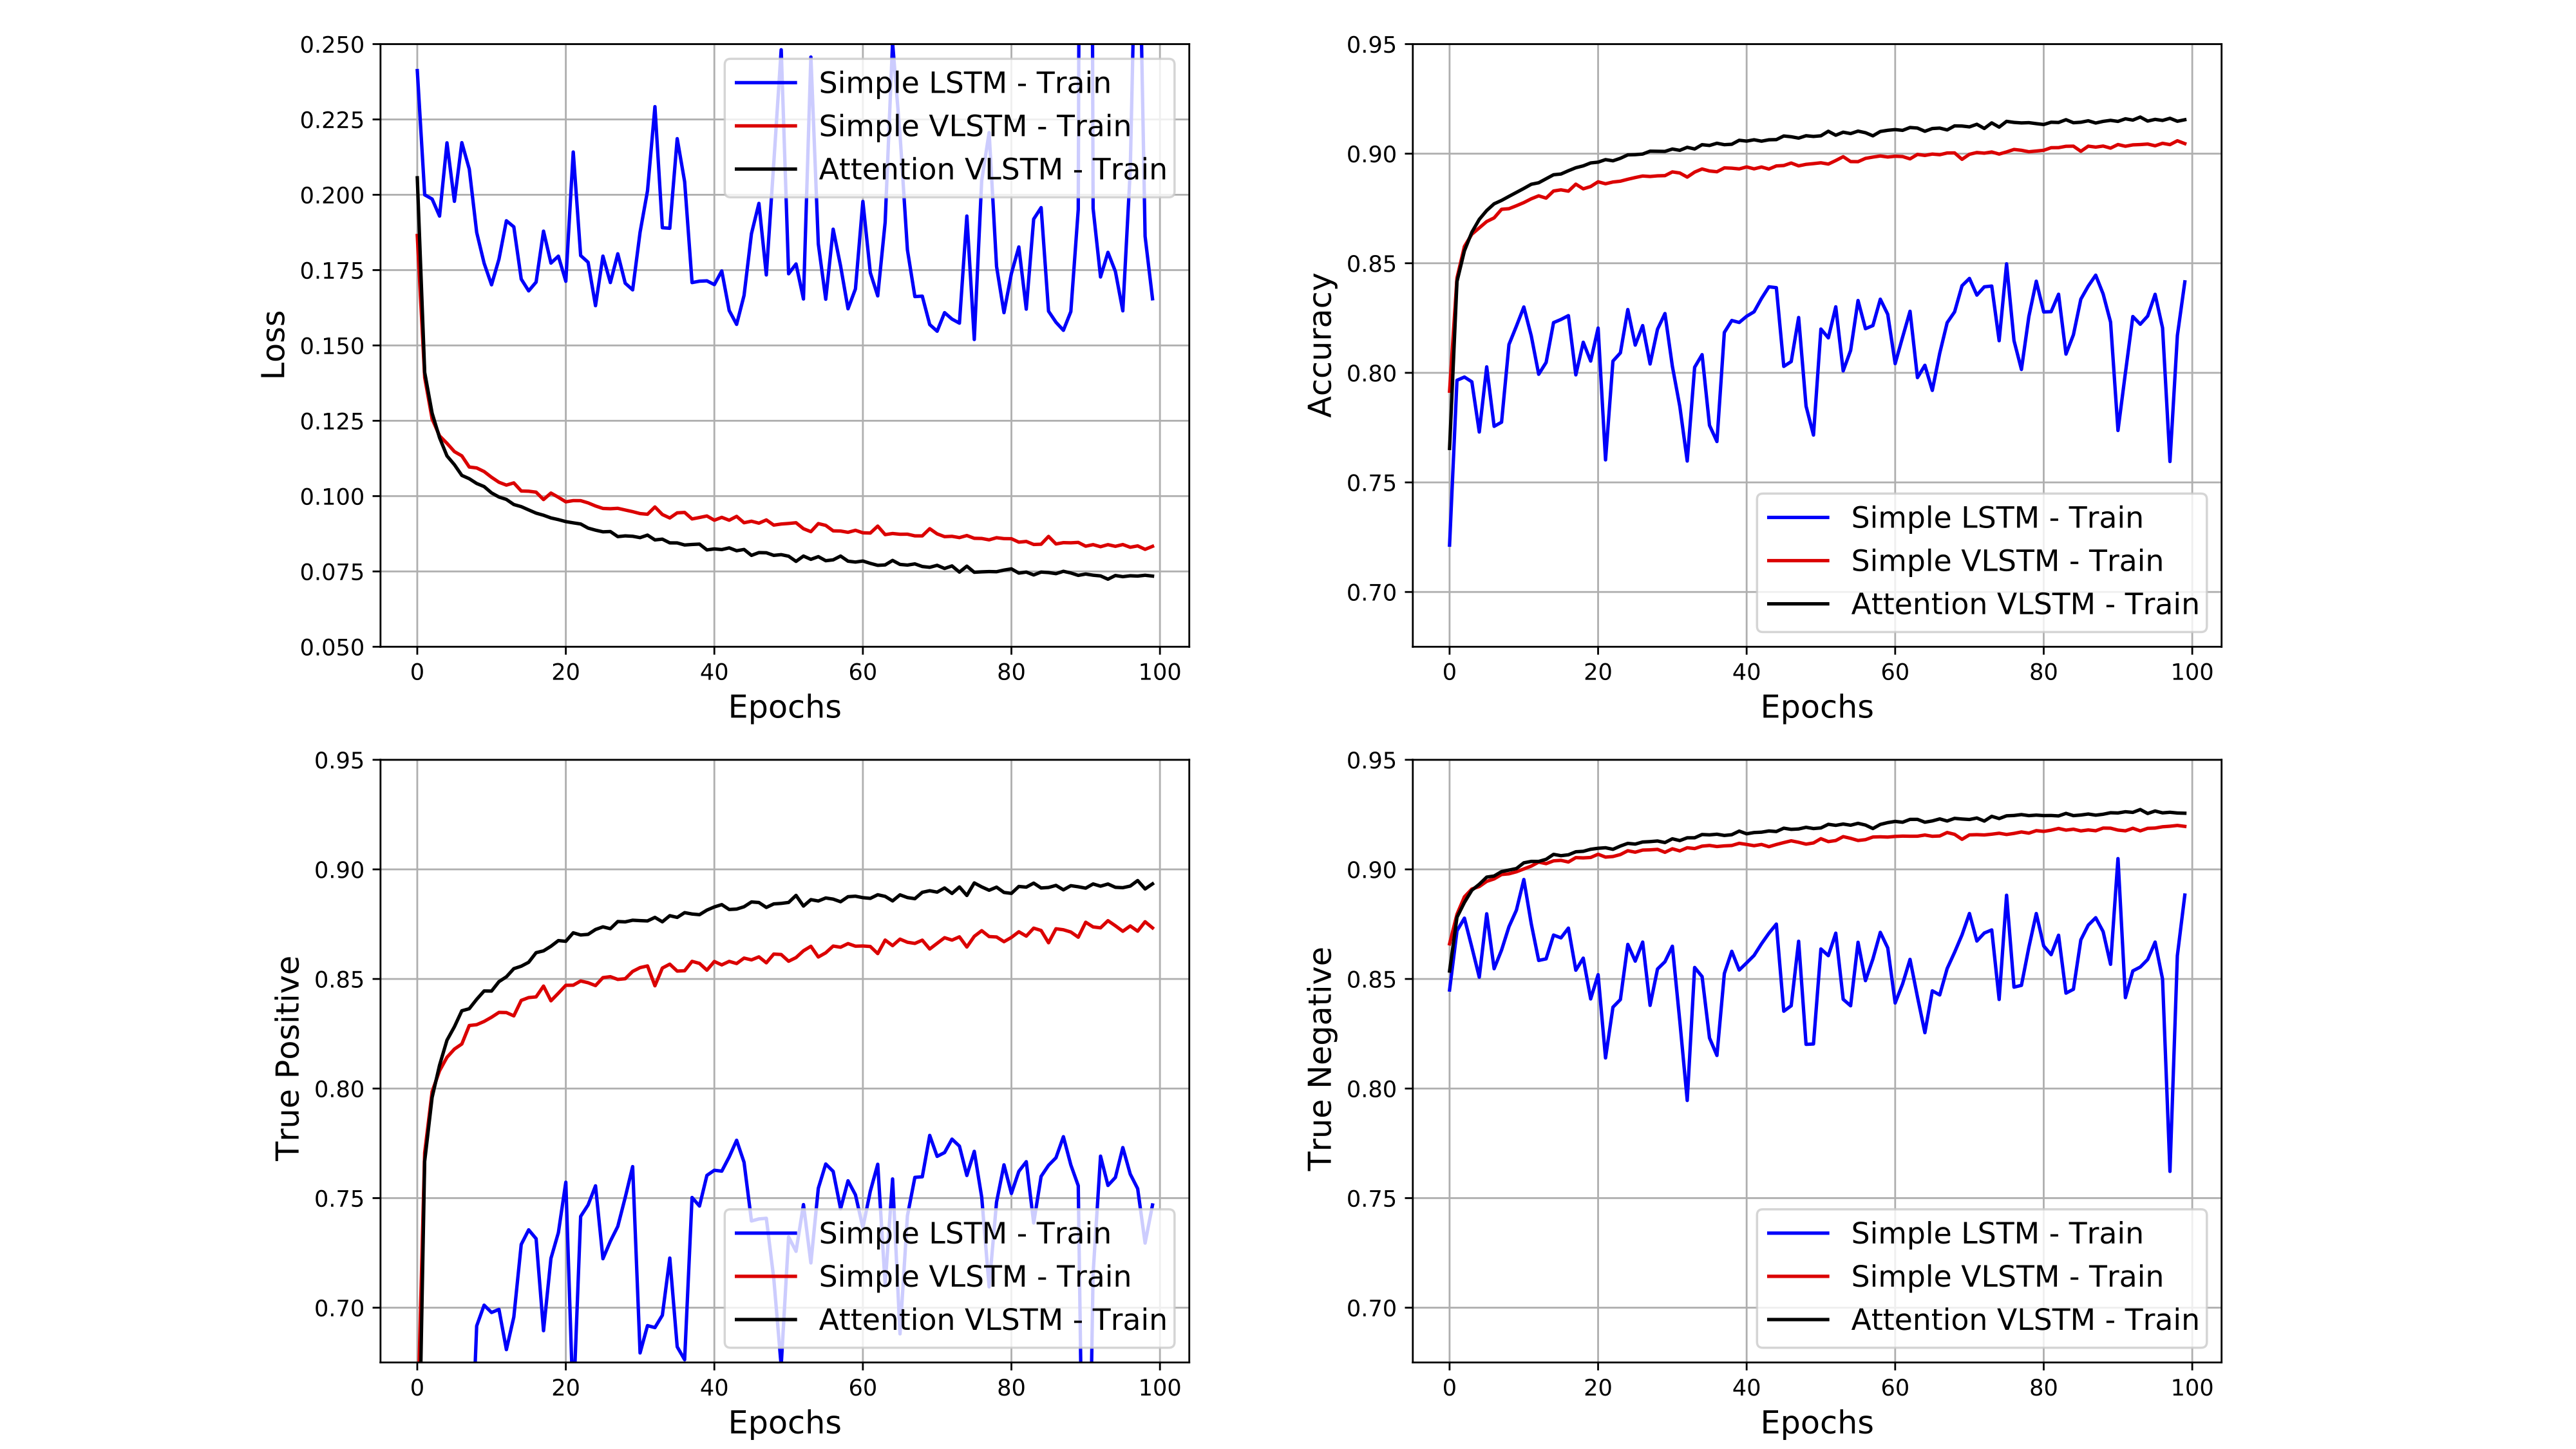
\includegraphics[trim = 100 0 100 0, width=1.0\textwidth, clip]{Figure/3Networks/3-4-3-1LSTMvsVLSTM.png}
 \caption[標準的なLSTMと独自のネットワークの比較]{標準的なLSTMと独自のネットワークの比較。左上が損失、右上が正答率、左下がTPR、右下がTNRである。それぞれ青線は標準的なLSTM、赤線は独自のLSTM、青線は独自のAttention LSTMについての結果を表している。}
 \label{3-4-3-1LSTMvsVLSTM}
\end{figure}

標準的なLSTMは系列の順序を重視しているため学習が安定していないことが分かる。
また、独自のネットワーク同士の比較においても、エンコーダー部からのコンテキストを受け取ることのできる独自のAttention LSTMの性能が高くなっている。
以上のことから、標準的なLSTMを単純に使うことは不適であり、独自のネットワーク構造による大幅な性能の改善が可能であると確認できる。\\

次に独自のAttention LSTMについての比較を行う。
ここでは訓練データをデータ属性毎に分離した。
ここでデータ属性とは終状態 ($\rm c\bar{c}$・$\rm b\bar{b}$) 、崩壊点のタネ (PV・SV) の4つである。
それぞれデータ属性のみで構成された訓練データで学習した特化型のネットワークを用意した。
それらのネットワークと全てのデータを使用した標準的なネットワークについての比較の結果を図\ref{3-4-3-2EfficiencyCurve}と図\ref{3-4-3-2ROCCurve}に示す。

\begin{itemize}
 \item ALL : 全てのデータを使用した標準的なネットワーク
 \item CC, BB : 終状態が$\rm c\bar{c}$、$\rm b\bar{b}$のデータのみを使用した特化型のネットワーク
 \item PV, SV : 崩壊点のタネがPV、SVのデータのみを使用した特化型のネットワーク
\end{itemize}

\begin{figure}[htbp]
 \centering
 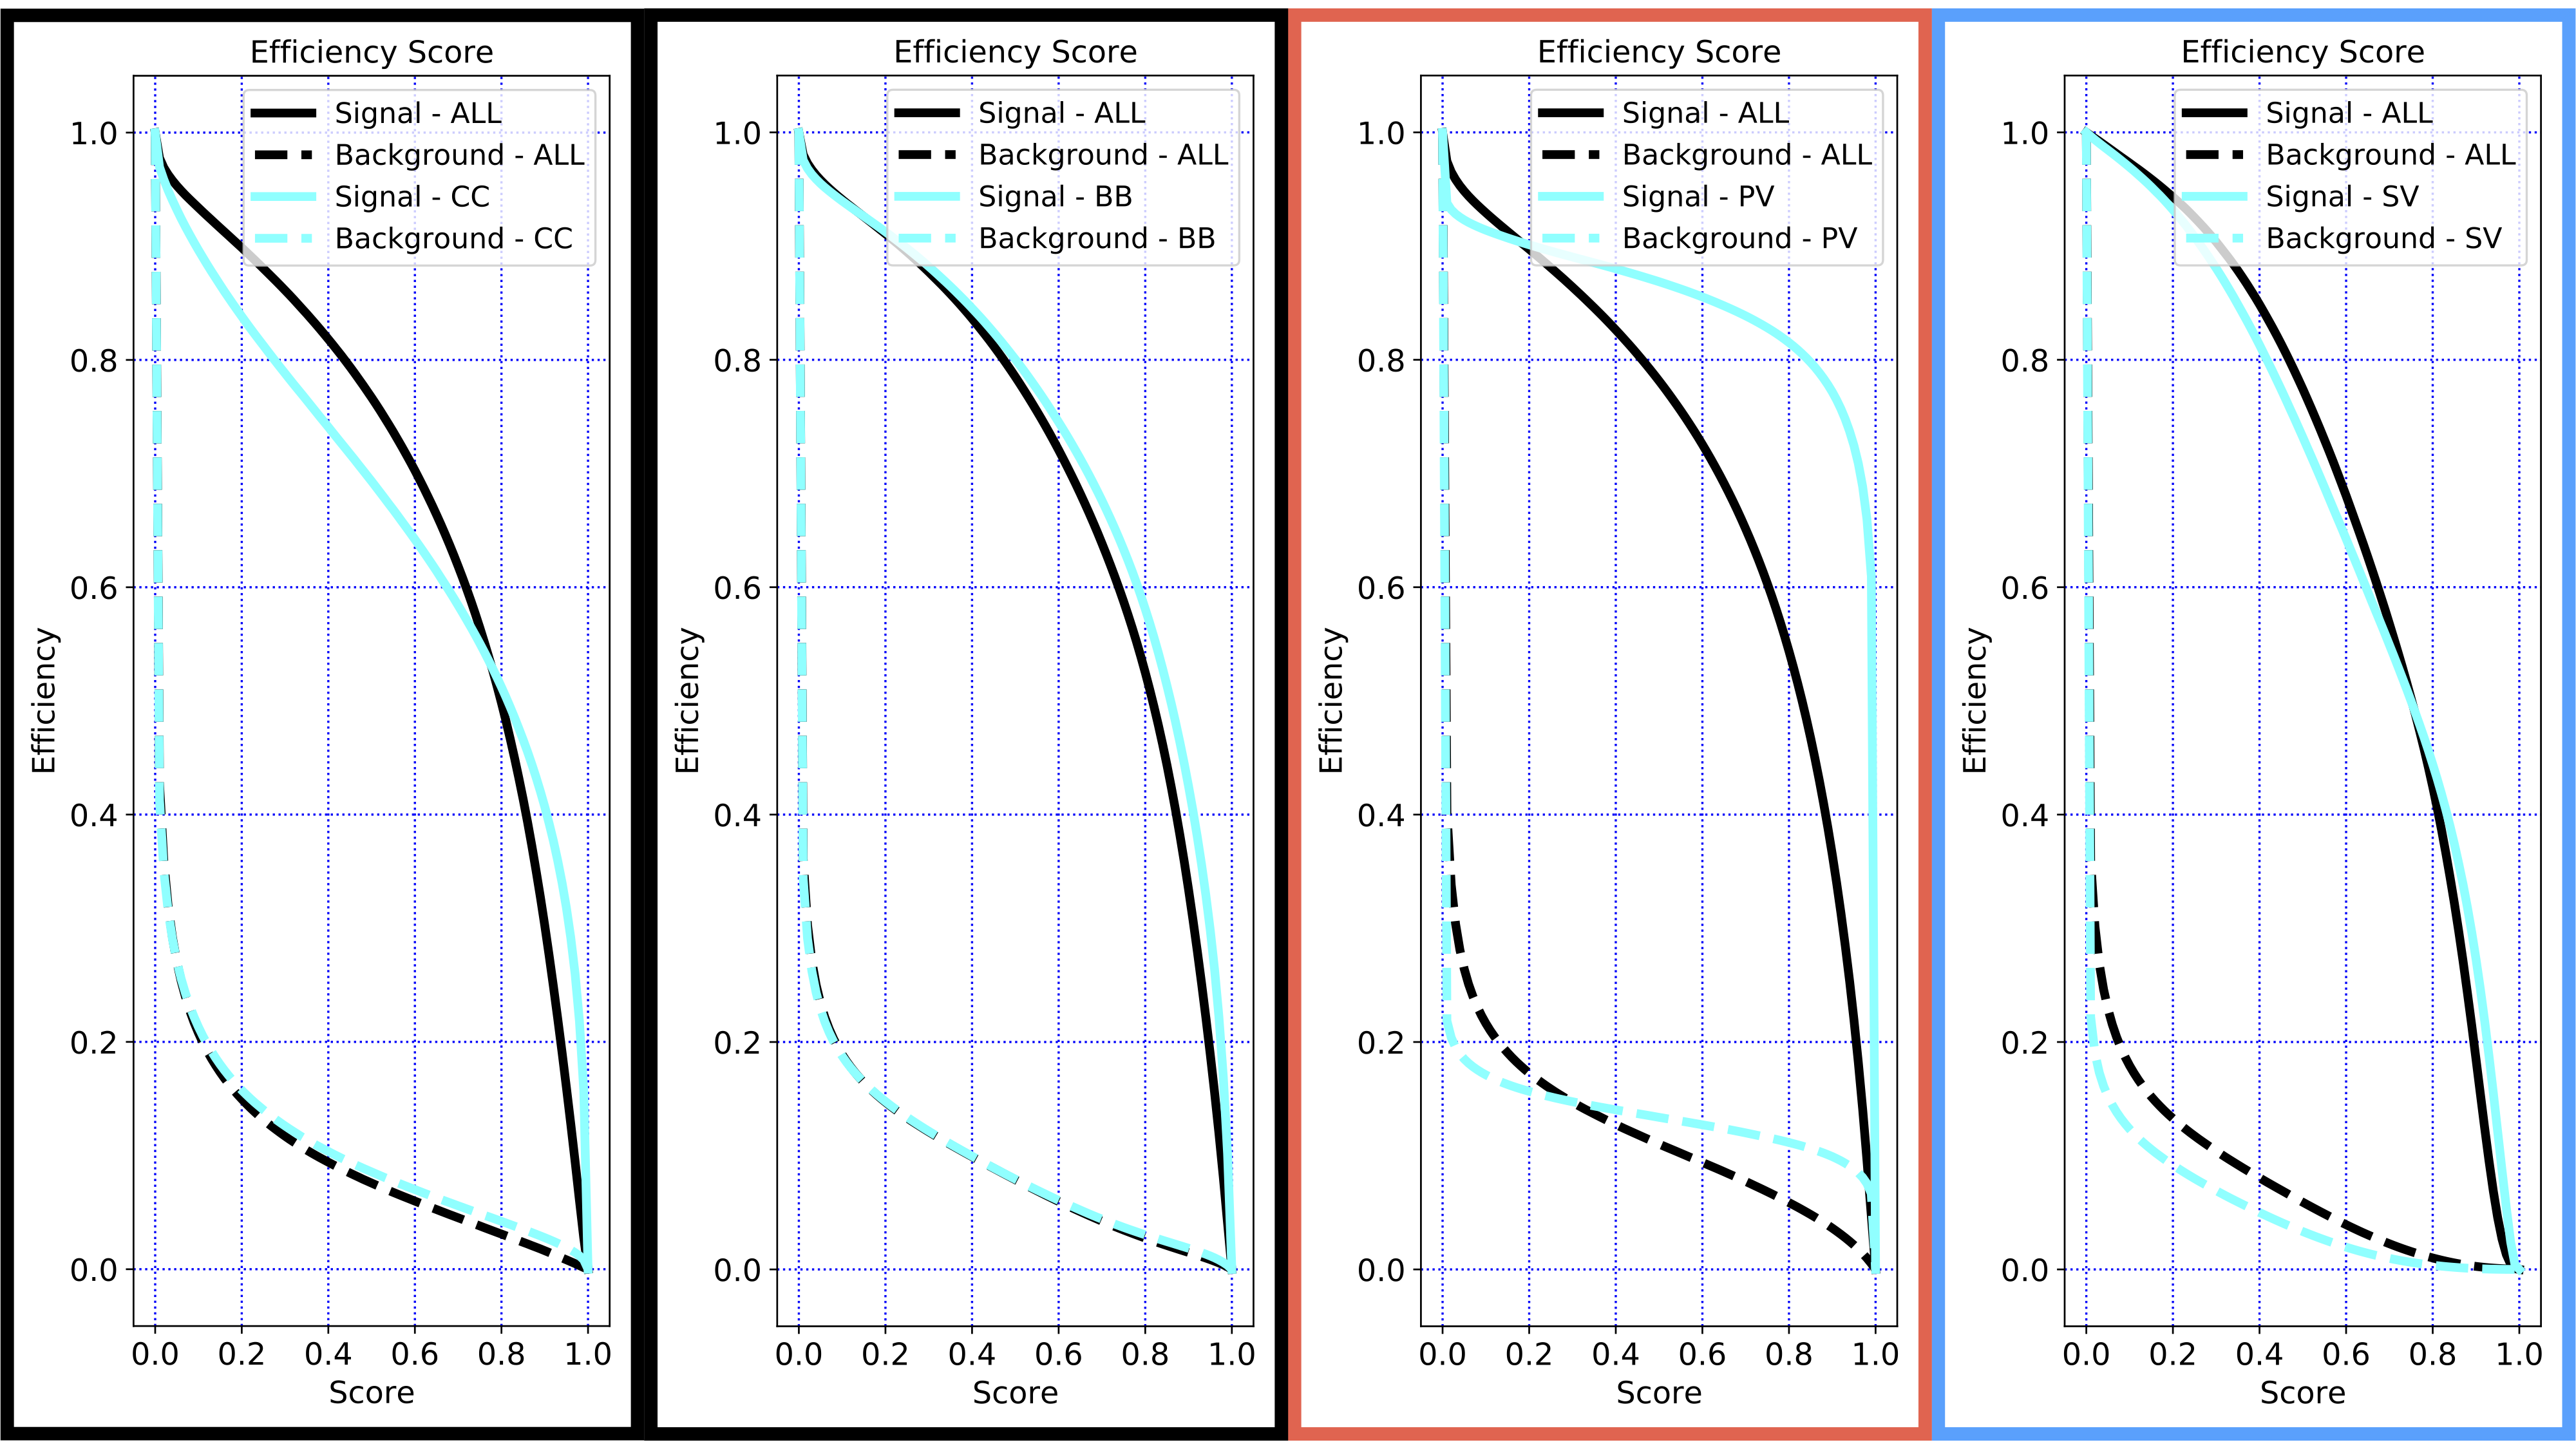
\includegraphics[width=1.0\textwidth, clip]{Figure/3Networks/3-4-3-2EfficiencyCurve.png}
 \caption[各データ属性の効率とスコアの関係]{各データ属性の効率とスコアの関係。縦軸は効率、横軸はネットワークのスコアについての閾値である。実線は信号効率、破線はバックグラウンド効率である。黒線は全データを使用した標準的なネットワーク、青線は個々の特化型のネットワークをそれぞれ表している。}
 \label{3-4-3-2EfficiencyCurve}
\end{figure}

\begin{figure}[htbp]
 \centering
 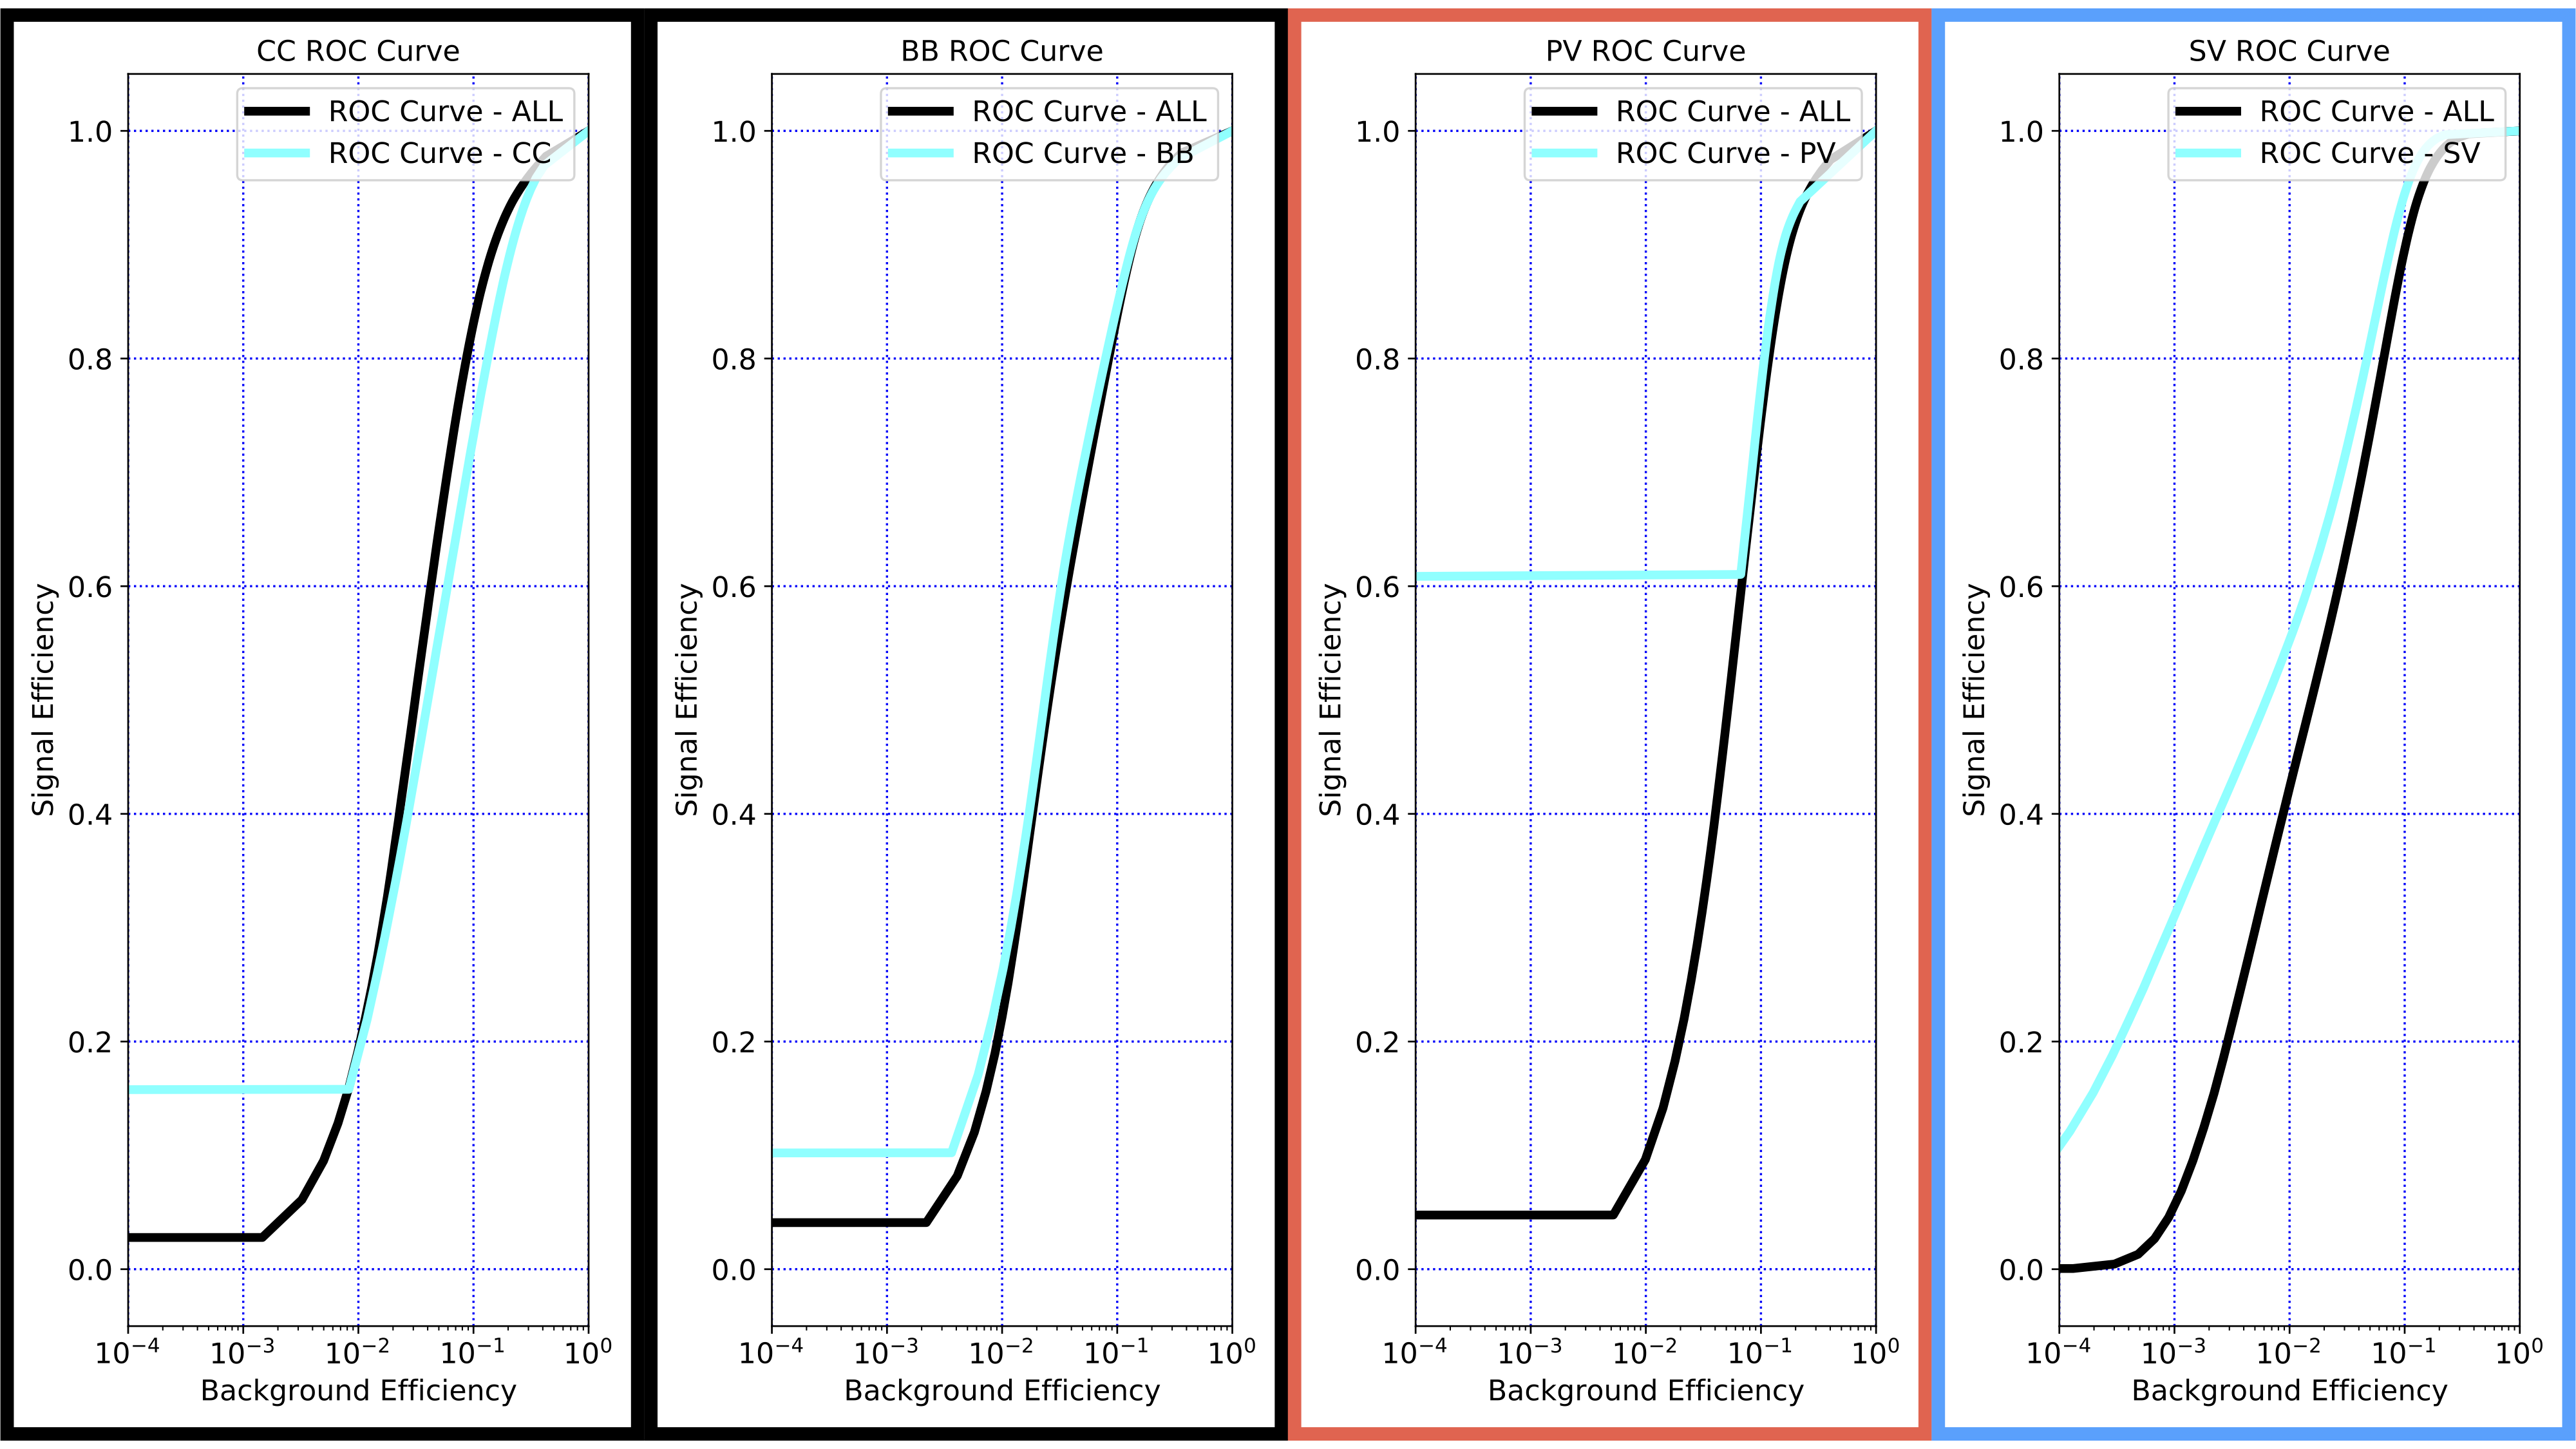
\includegraphics[width=1.0\textwidth, clip]{Figure/3Networks/3-4-3-2ROCCurve.png}
 \caption[各データ属性のROC曲線]{各データ属性のROC曲線。縦軸は信号効率、横軸はバックグラウンド効率である。黒線は全データを使用した標準的なネットワーク、青線は個々の特化型のネットワークをそれぞれ表している。}
 \label{3-4-3-2ROCCurve}
\end{figure}

比較に関してはROC曲線を使用している。
評価に際してのデータは特化型のネットワークの学習に使用した訓練データと同じ属性のものを用いた。
終状態$\rm c\bar{c}$や終状態$\rm b\bar{b}$に関しては基本的な性能の差がほとんどないと分かる。
したがって、個々の終状態のデータに関してはその特性に大きな差異は存在しないと判断できる。
各崩壊点のタネに特化したネットワークに関しては両者とも性能の向上が見られた。
特に、PVのタネに特化したネットワークは結合と非結合との分離が非常に良くできている。
ROC曲線ではSVに特化したネットワークが標準的なネットワークより大幅に性能が改善されていると分かる。\\

2. ネットワーク内の理解\\

飛跡対についてのネットワークとは異なり、任意の数の飛跡についてのネットワークはAttentionを持っている。
したがって、ネットワークの内部をAttention Weightを確認することによって、ネットワーク内部を把握することができる。
具体的には、エンコーダー部の飛跡がデコーダー部のどのような飛跡に注意し情報を受け取っているかを確認することが可能である。
そのようなAttention Weightについて、標準的なネットワークとPVのタネを用いて作成したサンプルを図\ref{3-4-3-3AttentionWeight}に示す。

図上部は横軸がデコーダー部の飛跡番号、縦軸がエンコーダー部の飛跡番号となっている。
ここではAttention Weightはカラースケールで表されている。
デコーダー部の飛跡によるAttention Weightの出力を縦方向に積んだような表現方法である。

図下部はエンコーダー部の飛跡を上に、デコーダー部の飛跡を下に並べた図となっている。
ここではAttention Weightは透過度で表現されている。
また、デコーダー部の飛跡の内、崩壊点のタネと結合しているものを赤、結合していないものを青で描画している。
デコーダー部の飛跡の数が少ないのはゼロ埋めを取り除いている為である。

これらの図から結合している飛跡はエンコーダー部の飛跡に注意し、結合していない飛跡はエンコーダー部のゼロ埋めに注意している傾向があると分かる。

\begin{figure}[htbp]
 \centering
  %\begin{tabular}{cccc}
   \begin{minipage}{1.0\textwidth}
    \centering
    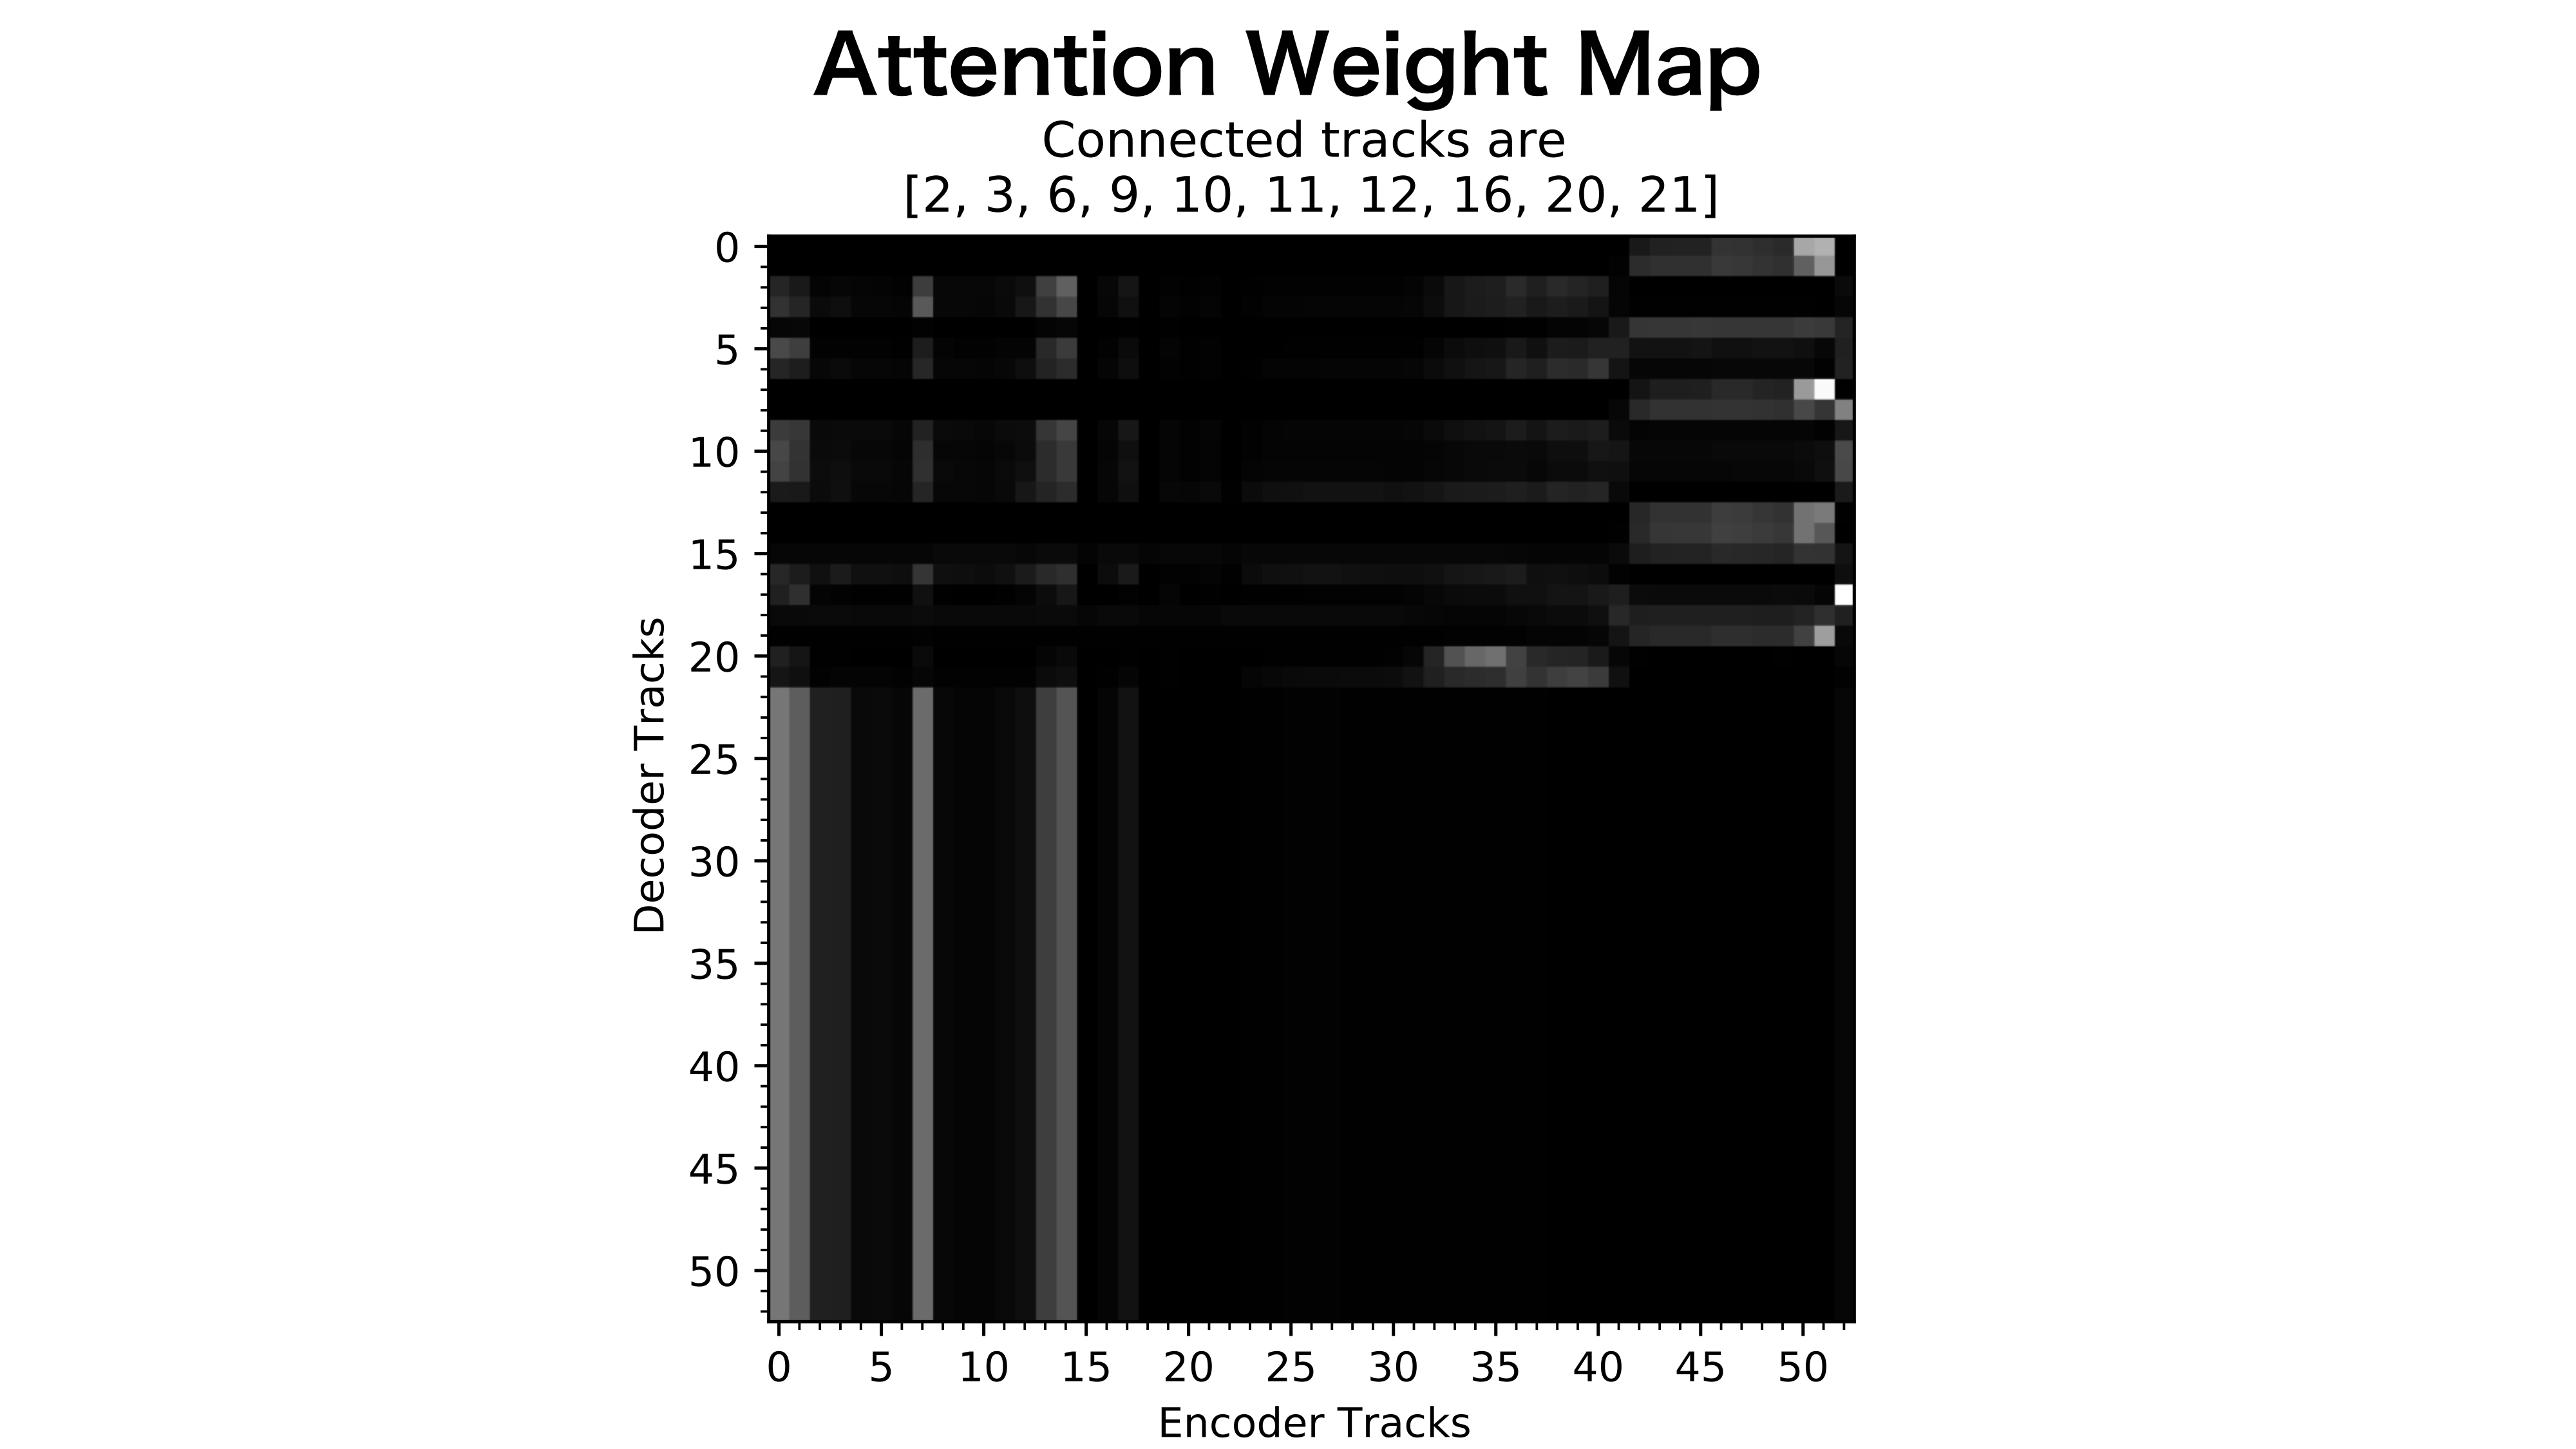
\includegraphics[trim = 200 0 200 0, width=1.0\textwidth, clip]{Figure/3Networks/3-4-3-3AttentionWeightMap.png}
    %\subcaption{終状態$\rm c\bar{c}$に特化したネットワーク}
    %\label{3-4-3-3AttentionWeightMap}
   \end{minipage}
   
   \begin{minipage}{1.0\textwidth}
   \centering
    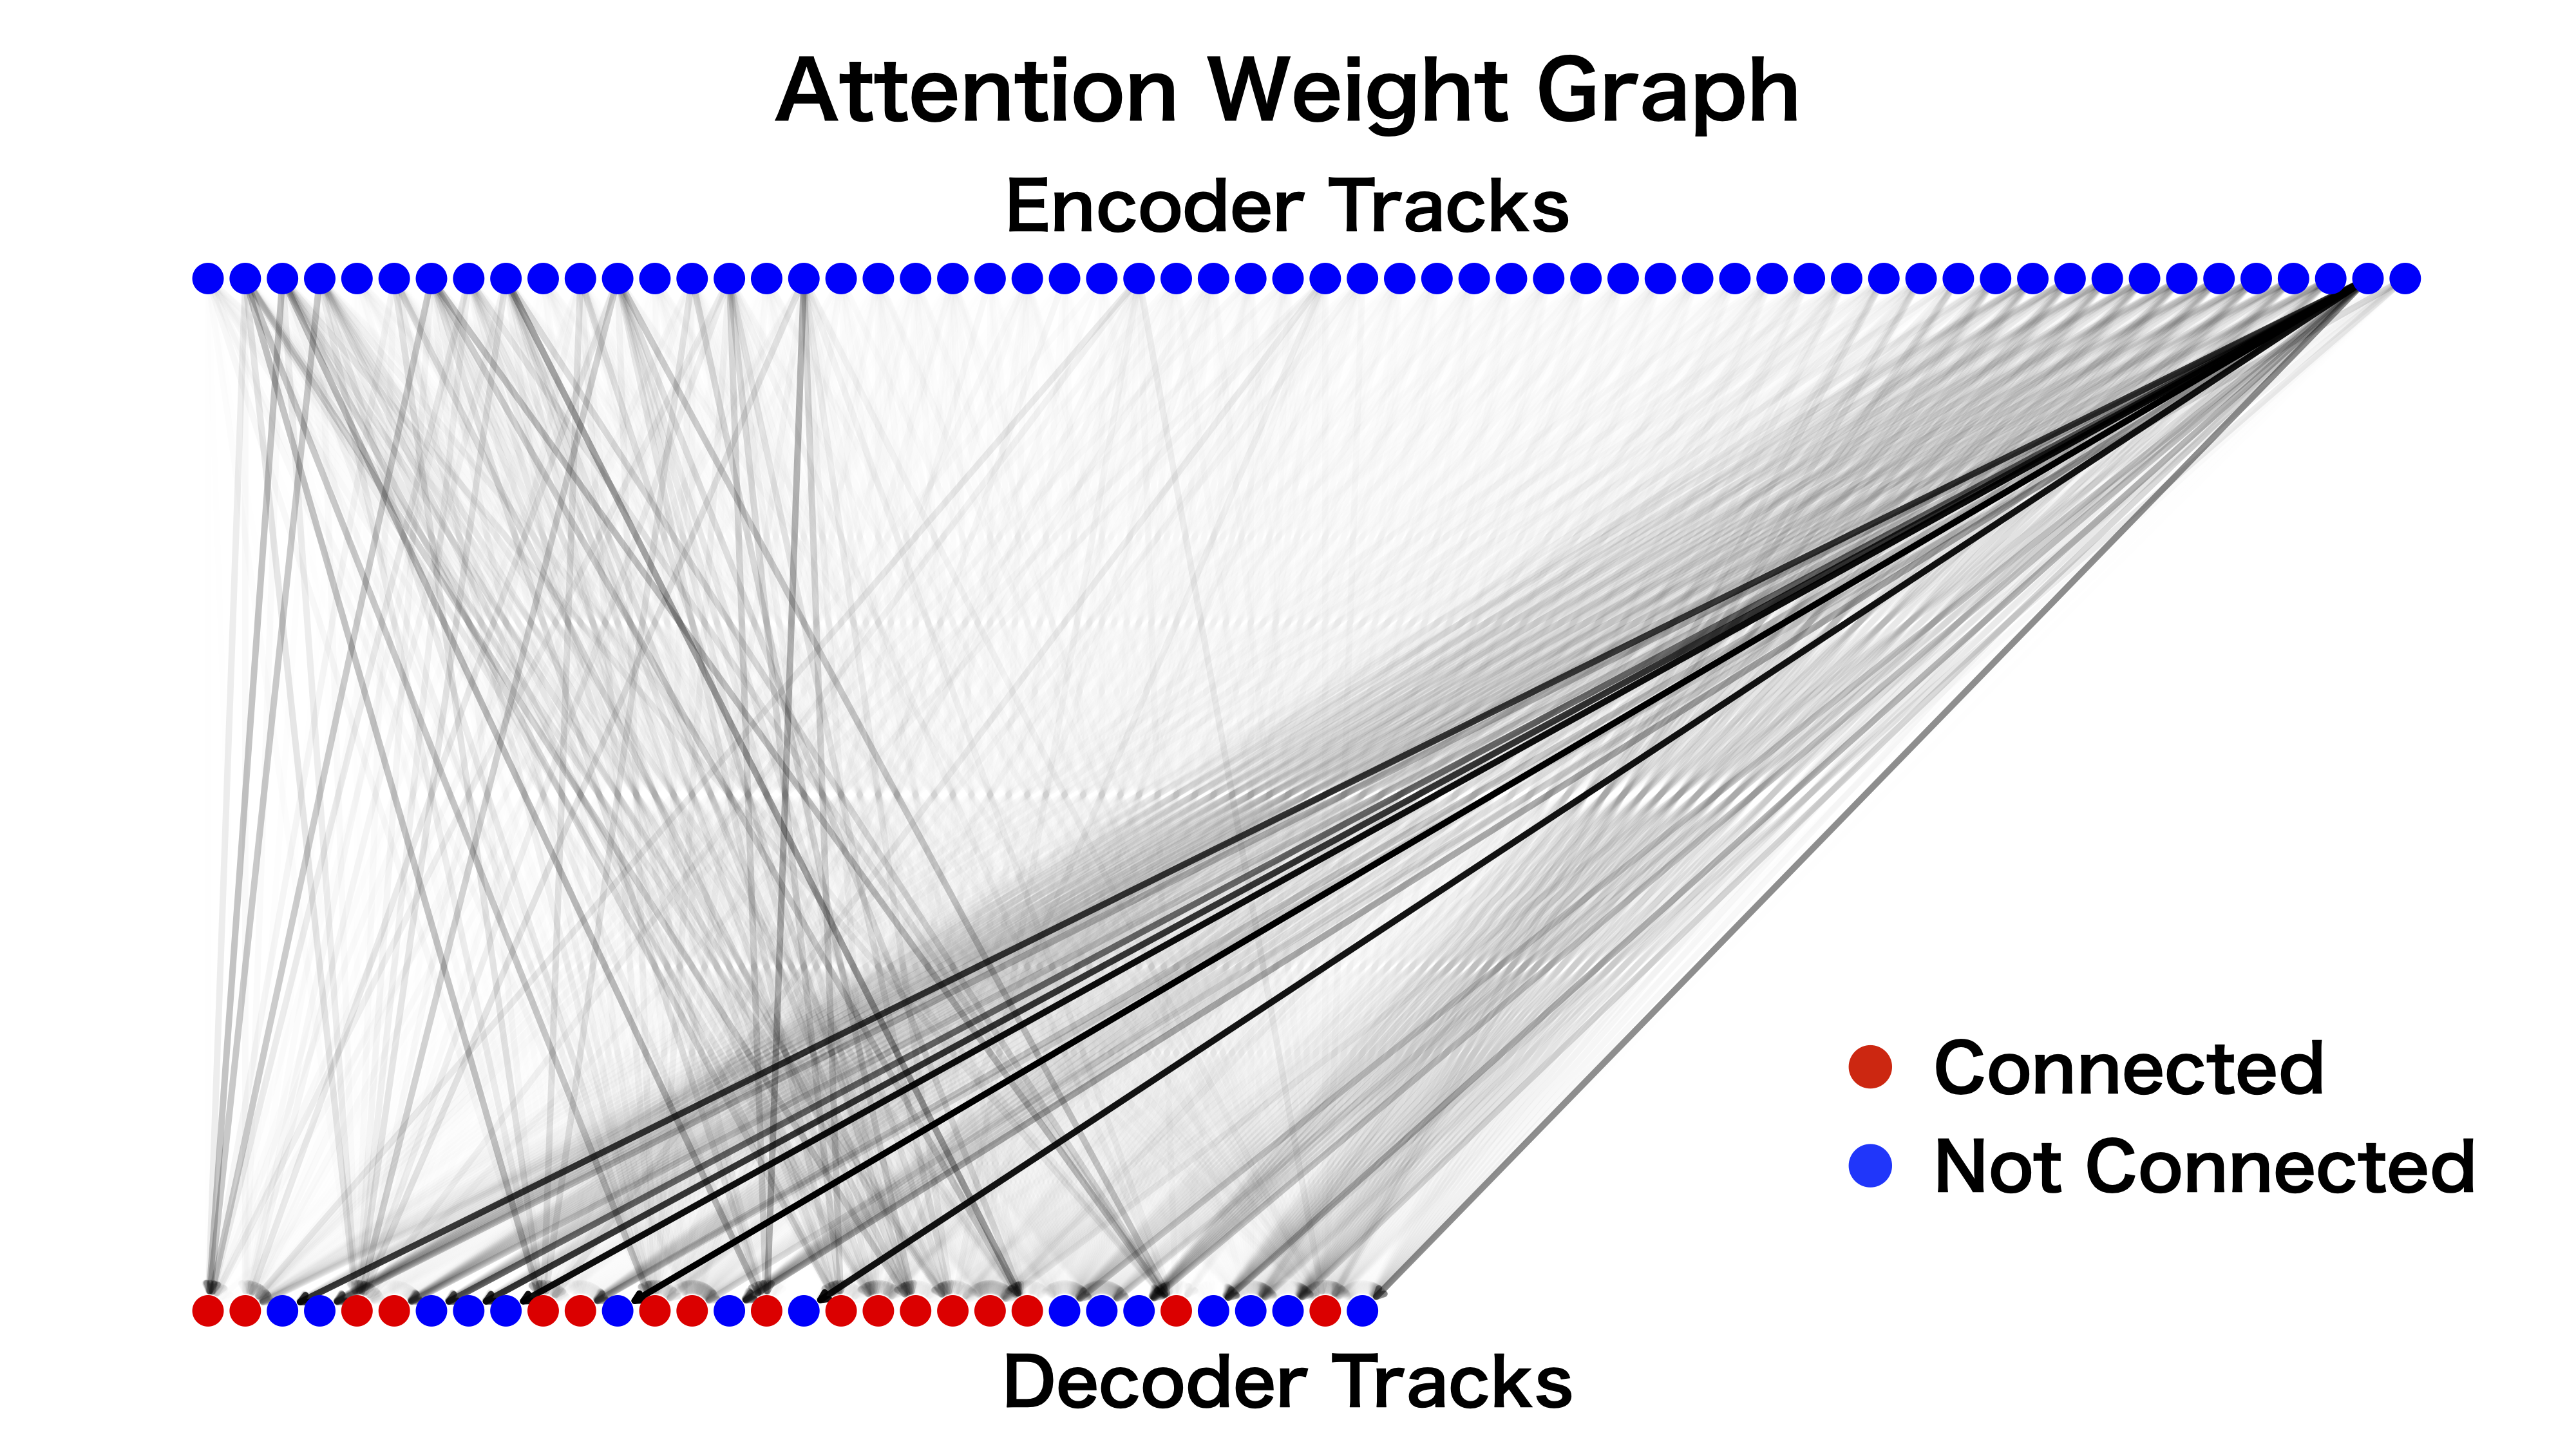
\includegraphics[trim = 100 0 100 0, width=1.0\textwidth, clip]{Figure/3Networks/3-4-3-3AttentionWeightGraph.png}
    %\subcaption{終状態$\rm b\bar{b}$に特化したネットワーク}
    %\label{3-4-3-3AttentionWeightGraph}
   \end{minipage}
  \caption[Attention Weight]{図上部はAttention Weightを行列として表現した図、図下部はAttention Weightをより直感的に示した図である。図上部では縦軸がデコーダーの飛跡番号、横軸がエンコーダーの飛跡番号となっている。また、カラースケールはAttention Weightである。図下部では上段にデコーダーの飛跡、下段にデコーダーの飛跡を描画している。デコーダーの飛跡ではタネと結合している飛跡については赤丸を使用している。}
  \label{3-4-3-3AttentionWeight}
 %\end{tabular}
\end{figure}



























